\documentclass[pdftex]{beamer}
\usepackage{graphicx}
\usepackage{tikz, ifthen, xcolor, pgfplots}
\usepackage{amsmath}

\usetikzlibrary{shapes.misc}

\newcommand{\unitsize}{0.25cm}

\tikzset{cross/.style={cross out, draw=black, minimum size=2*(#1-\pgflinewidth), inner sep=0pt, outer sep=0pt},
%default radius will be 1pt. 
cross/.default={1pt}}

\setlength{\rightskip}{0pt} % I want justifed text
\sloppy

\mode<presentation> {
  \usetheme{Darmstadt}
  \setbeamercovered{highly dynamic}
}

\usepackage[english]{babel}
\usepackage[utf8]{inputenc}
\usepackage[T1]{fontenc}

\DeclareMathOperator{\mv}{move}
\DeclareMathOperator{\dt}{dot}
\DeclareMathOperator{\area}{area}
\DeclareMathOperator{\boundary}{boundary}

\title{$485$ - a new upper bound for Morpion Solitaire}

\author[H.~Michalewski, A.~Nagórko, J.~Pawlewicz]{Henryk Michalewski, Andrzej~Nag\'orko, Jakub Pawlewicz}

\institute[Warsaw]
{
University of Warsaw
}

\date[July 2015]{Computer Games Workshop\\\vspace{3mm} IJCAI 2015}

\begin{document}

\begin{frame}[plain]
  \titlepage

  % Abstract
\end{frame}

%%%%
%
% Introduction
%
%%%%

\section{Morpion Solitaire}
\subsection{Rules}

\begin{frame}
\frametitle{Morpion Solitaire}

\begin{itemize}
\item A single-player paper-and-pencil game

\vspace{3mm}
{\footnotesize The goal is to find longest possible sequence of valid moves.}

\vspace{8mm}
\item Popularized in France in 70's by {\em Science \& Vie} magazine

\vspace{3mm}
{\footnotesize The magazine published long sequences found by its readers.}

\vspace{8mm}
\item Difficult for computers. 

\vspace{3mm}
{\footnotesize The human record was obtained by C.-H. Bruneau in $1976$.

\vspace{1mm}
It was beat by NRPA (Monte Carlo) algorithm by Ch. Rosin in $2010$.

\vspace{1mm}
Rosin got best paper award at IJCAI 2011 for this work.
}
\end{itemize}

\end{frame}

\begin{frame}
\frametitle{Rules of Morpion Solitaire}
\begin{center}

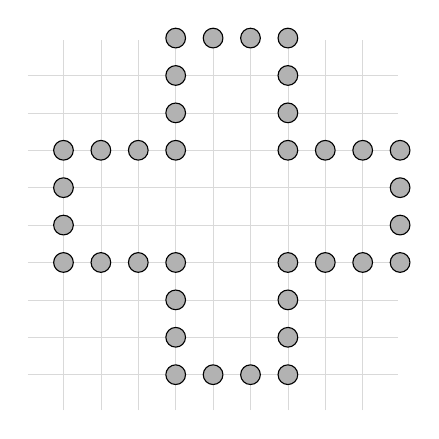
\begin{tikzpicture}[scale=0.95]
\draw[step=2*\unitsize,gray!30,very thin,shift={(-\unitsize, -\unitsize)}] (-9.900000*\unitsize,-9.900000*\unitsize) grid (9.900000*\unitsize,9.900000*\unitsize);
\tikzstyle{every node}=[draw,
			circle,
			fill=white,
			minimum size  = 1*\unitsize,
			node distance = 2*\unitsize,
			inner sep=0pt
			] 


\node[fill=black!30, thin] at (3*\unitsize,9*\unitsize) {};
        

\node[fill=black!30, thin] at (3*\unitsize,7*\unitsize) {};
        

\node[fill=black!30, thin] at (3*\unitsize,5*\unitsize) {};
        

\node[fill=black!30, thin] at (3*\unitsize,3*\unitsize) {};
        

\node[fill=black!30, thin] at (5*\unitsize,3*\unitsize) {};
        

\node[fill=black!30, thin] at (7*\unitsize,3*\unitsize) {};
        

\node[fill=black!30, thin] at (9*\unitsize,3*\unitsize) {};
        

\node[fill=black!30, thin] at (9*\unitsize,1*\unitsize) {};
        

\node[fill=black!30, thin] at (9*\unitsize,-1*\unitsize) {};
        

\node[fill=black!30, thin] at (9*\unitsize,-3*\unitsize) {};
        

\node[fill=black!30, thin] at (7*\unitsize,-3*\unitsize) {};
        

\node[fill=black!30, thin] at (5*\unitsize,-3*\unitsize) {};
        

\node[fill=black!30, thin] at (3*\unitsize,-3*\unitsize) {};
        

\node[fill=black!30, thin] at (3*\unitsize,-5*\unitsize) {};
        

\node[fill=black!30, thin] at (3*\unitsize,-7*\unitsize) {};
        

\node[fill=black!30, thin] at (3*\unitsize,-9*\unitsize) {};
        

\node[fill=black!30, thin] at (1*\unitsize,-9*\unitsize) {};
        

\node[fill=black!30, thin] at (-1*\unitsize,-9*\unitsize) {};
        

\node[fill=black!30, thin] at (-3*\unitsize,-9*\unitsize) {};
        

\node[fill=black!30, thin] at (-3*\unitsize,-7*\unitsize) {};
        

\node[fill=black!30, thin] at (-3*\unitsize,-5*\unitsize) {};
        

\node[fill=black!30, thin] at (-3*\unitsize,-3*\unitsize) {};
        

\node[fill=black!30, thin] at (-5*\unitsize,-3*\unitsize) {};
        

\node[fill=black!30, thin] at (-7*\unitsize,-3*\unitsize) {};
        

\node[fill=black!30, thin] at (-9*\unitsize,-3*\unitsize) {};
        

\node[fill=black!30, thin] at (-9*\unitsize,-1*\unitsize) {};
        

\node[fill=black!30, thin] at (-9*\unitsize,1*\unitsize) {};
        

\node[fill=black!30, thin] at (-9*\unitsize,3*\unitsize) {};
        

\node[fill=black!30, thin] at (-7*\unitsize,3*\unitsize) {};
        

\node[fill=black!30, thin] at (-5*\unitsize,3*\unitsize) {};
        

\node[fill=black!30, thin] at (-3*\unitsize,3*\unitsize) {};
        

\node[fill=black!30, thin] at (-3*\unitsize,5*\unitsize) {};
        

\node[fill=black!30, thin] at (-3*\unitsize,7*\unitsize) {};
        

\node[fill=black!30, thin] at (-3*\unitsize,9*\unitsize) {};
        

\node[fill=black!30, thin] at (-1*\unitsize,9*\unitsize) {};
        

\node[fill=black!30, thin] at (1*\unitsize,9*\unitsize) {};
        

\end{tikzpicture}



Initial position: $36$ dots arranged in a cross on a square grid.
\end{center}
\end{frame}

\begin{frame}
\frametitle{Rules of Morpion Solitaire}
\begin{center}

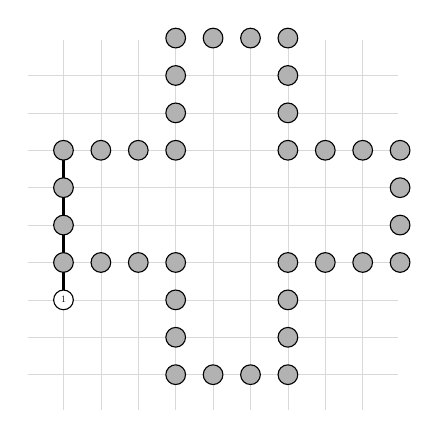
\begin{tikzpicture}[scale=0.95]
\draw[step=2*\unitsize,gray!30,very thin,shift={(-\unitsize, -\unitsize)}] (-9.900000*\unitsize,-9.900000*\unitsize) grid (9.900000*\unitsize,9.900000*\unitsize);
\tikzstyle{every node}=[draw,
			circle,
			fill=white,
			minimum size  = 1*\unitsize,
			node distance = 2*\unitsize,
			inner sep=0pt
			] 


\draw[thick] (-9*\unitsize,-1*\unitsize) -- (-9*\unitsize,1*\unitsize);
    

\draw[thick] (-9*\unitsize,1*\unitsize) -- (-9*\unitsize,3*\unitsize);
    

\draw[thick] (-9*\unitsize,-1*\unitsize) -- (-9*\unitsize,-3*\unitsize);
    

\draw[thick] (-9*\unitsize,-3*\unitsize) -- (-9*\unitsize,-5*\unitsize);
    

\node[fill=black!30, thin] at (3*\unitsize,9*\unitsize) {};
        

\node[fill=black!30, thin] at (3*\unitsize,7*\unitsize) {};
        

\node[fill=black!30, thin] at (3*\unitsize,5*\unitsize) {};
        

\node[fill=black!30, thin] at (3*\unitsize,3*\unitsize) {};
        

\node[fill=black!30, thin] at (5*\unitsize,3*\unitsize) {};
        

\node[fill=black!30, thin] at (7*\unitsize,3*\unitsize) {};
        

\node[fill=black!30, thin] at (9*\unitsize,3*\unitsize) {};
        

\node[fill=black!30, thin] at (9*\unitsize,1*\unitsize) {};
        

\node[fill=black!30, thin] at (9*\unitsize,-1*\unitsize) {};
        

\node[fill=black!30, thin] at (9*\unitsize,-3*\unitsize) {};
        

\node[fill=black!30, thin] at (7*\unitsize,-3*\unitsize) {};
        

\node[fill=black!30, thin] at (5*\unitsize,-3*\unitsize) {};
        

\node[fill=black!30, thin] at (3*\unitsize,-3*\unitsize) {};
        

\node[fill=black!30, thin] at (3*\unitsize,-5*\unitsize) {};
        

\node[fill=black!30, thin] at (3*\unitsize,-7*\unitsize) {};
        

\node[fill=black!30, thin] at (3*\unitsize,-9*\unitsize) {};
        

\node[fill=black!30, thin] at (1*\unitsize,-9*\unitsize) {};
        

\node[fill=black!30, thin] at (-1*\unitsize,-9*\unitsize) {};
        

\node[fill=black!30, thin] at (-3*\unitsize,-9*\unitsize) {};
        

\node[fill=black!30, thin] at (-3*\unitsize,-7*\unitsize) {};
        

\node[fill=black!30, thin] at (-3*\unitsize,-5*\unitsize) {};
        

\node[fill=black!30, thin] at (-3*\unitsize,-3*\unitsize) {};
        

\node[fill=black!30, thin] at (-5*\unitsize,-3*\unitsize) {};
        

\node[fill=black!30, thin] at (-7*\unitsize,-3*\unitsize) {};
        

\node[fill=black!30, thin] at (-9*\unitsize,-3*\unitsize) {};
        

\node[fill=black!30, thin] at (-9*\unitsize,-1*\unitsize) {};
        

\node[fill=black!30, thin] at (-9*\unitsize,1*\unitsize) {};
        

\node[fill=black!30, thin] at (-9*\unitsize,3*\unitsize) {};
        

\node[fill=black!30, thin] at (-7*\unitsize,3*\unitsize) {};
        

\node[fill=black!30, thin] at (-5*\unitsize,3*\unitsize) {};
        

\node[fill=black!30, thin] at (-3*\unitsize,3*\unitsize) {};
        

\node[fill=black!30, thin] at (-3*\unitsize,5*\unitsize) {};
        

\node[fill=black!30, thin] at (-3*\unitsize,7*\unitsize) {};
        

\node[fill=black!30, thin] at (-3*\unitsize,9*\unitsize) {};
        

\node[fill=black!30, thin] at (-1*\unitsize,9*\unitsize) {};
        

\node[fill=black!30, thin] at (1*\unitsize,9*\unitsize) {};
        

\node[thin] at (-9*\unitsize,-5*\unitsize)  {\scalebox{0.35}{1}};
            

\end{tikzpicture}



A move: place a dot and draw a line (diagonal, horizontal or vertical) passing through the placed dot and four others.
\end{center}
\end{frame}

\begin{frame}
\frametitle{Rules of Morpion Solitaire}
\begin{center}

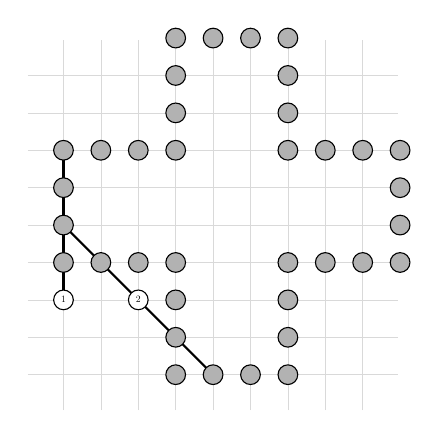
\begin{tikzpicture}[scale=0.95]
\draw[step=2*\unitsize,gray!30,very thin,shift={(-\unitsize, -\unitsize)}] (-9.900000*\unitsize,-9.900000*\unitsize) grid (9.900000*\unitsize,9.900000*\unitsize);
\tikzstyle{every node}=[draw,
			circle,
			fill=white,
			minimum size  = 1*\unitsize,
			node distance = 2*\unitsize,
			inner sep=0pt
			] 


\draw[thick] (-9*\unitsize,-1*\unitsize) -- (-9*\unitsize,1*\unitsize);
    

\draw[thick] (-9*\unitsize,1*\unitsize) -- (-9*\unitsize,3*\unitsize);
    

\draw[thick] (-9*\unitsize,-1*\unitsize) -- (-9*\unitsize,-3*\unitsize);
    

\draw[thick] (-9*\unitsize,-3*\unitsize) -- (-9*\unitsize,-5*\unitsize);
    

\draw[thick] (-5*\unitsize,-5*\unitsize) -- (-3*\unitsize,-7*\unitsize);
    

\draw[thick] (-3*\unitsize,-7*\unitsize) -- (-1*\unitsize,-9*\unitsize);
    

\draw[thick] (-5*\unitsize,-5*\unitsize) -- (-7*\unitsize,-3*\unitsize);
    

\draw[thick] (-7*\unitsize,-3*\unitsize) -- (-9*\unitsize,-1*\unitsize);
    

\node[fill=black!30, thin] at (3*\unitsize,9*\unitsize) {};
        

\node[fill=black!30, thin] at (3*\unitsize,7*\unitsize) {};
        

\node[fill=black!30, thin] at (3*\unitsize,5*\unitsize) {};
        

\node[fill=black!30, thin] at (3*\unitsize,3*\unitsize) {};
        

\node[fill=black!30, thin] at (5*\unitsize,3*\unitsize) {};
        

\node[fill=black!30, thin] at (7*\unitsize,3*\unitsize) {};
        

\node[fill=black!30, thin] at (9*\unitsize,3*\unitsize) {};
        

\node[fill=black!30, thin] at (9*\unitsize,1*\unitsize) {};
        

\node[fill=black!30, thin] at (9*\unitsize,-1*\unitsize) {};
        

\node[fill=black!30, thin] at (9*\unitsize,-3*\unitsize) {};
        

\node[fill=black!30, thin] at (7*\unitsize,-3*\unitsize) {};
        

\node[fill=black!30, thin] at (5*\unitsize,-3*\unitsize) {};
        

\node[fill=black!30, thin] at (3*\unitsize,-3*\unitsize) {};
        

\node[fill=black!30, thin] at (3*\unitsize,-5*\unitsize) {};
        

\node[fill=black!30, thin] at (3*\unitsize,-7*\unitsize) {};
        

\node[fill=black!30, thin] at (3*\unitsize,-9*\unitsize) {};
        

\node[fill=black!30, thin] at (1*\unitsize,-9*\unitsize) {};
        

\node[fill=black!30, thin] at (-1*\unitsize,-9*\unitsize) {};
        

\node[fill=black!30, thin] at (-3*\unitsize,-9*\unitsize) {};
        

\node[fill=black!30, thin] at (-3*\unitsize,-7*\unitsize) {};
        

\node[fill=black!30, thin] at (-3*\unitsize,-5*\unitsize) {};
        

\node[fill=black!30, thin] at (-3*\unitsize,-3*\unitsize) {};
        

\node[fill=black!30, thin] at (-5*\unitsize,-3*\unitsize) {};
        

\node[fill=black!30, thin] at (-7*\unitsize,-3*\unitsize) {};
        

\node[fill=black!30, thin] at (-9*\unitsize,-3*\unitsize) {};
        

\node[fill=black!30, thin] at (-9*\unitsize,-1*\unitsize) {};
        

\node[fill=black!30, thin] at (-9*\unitsize,1*\unitsize) {};
        

\node[fill=black!30, thin] at (-9*\unitsize,3*\unitsize) {};
        

\node[fill=black!30, thin] at (-7*\unitsize,3*\unitsize) {};
        

\node[fill=black!30, thin] at (-5*\unitsize,3*\unitsize) {};
        

\node[fill=black!30, thin] at (-3*\unitsize,3*\unitsize) {};
        

\node[fill=black!30, thin] at (-3*\unitsize,5*\unitsize) {};
        

\node[fill=black!30, thin] at (-3*\unitsize,7*\unitsize) {};
        

\node[fill=black!30, thin] at (-3*\unitsize,9*\unitsize) {};
        

\node[fill=black!30, thin] at (-1*\unitsize,9*\unitsize) {};
        

\node[fill=black!30, thin] at (1*\unitsize,9*\unitsize) {};
        

\node[thin] at (-9*\unitsize,-5*\unitsize)  {\scalebox{0.35}{1}};
            

\node[thin] at (-5*\unitsize,-5*\unitsize)  {\scalebox{0.35}{2}};
            

\end{tikzpicture}



Two lines may cross, but they may not overlap.
\end{center}
\end{frame}

\begin{frame}
\frametitle{Rules of Morpion Solitaire}
\begin{center}

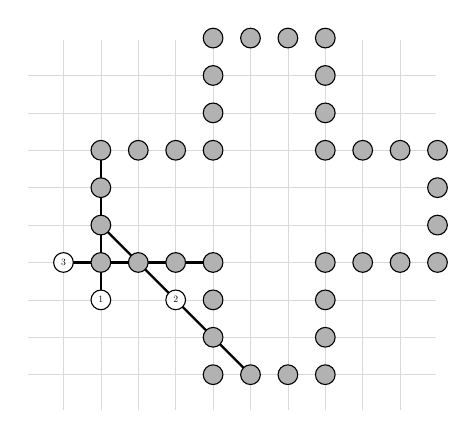
\begin{tikzpicture}[scale=0.95]
\draw[step=2*\unitsize,gray!30,very thin,shift={(-\unitsize, -\unitsize)}] (-11.900000*\unitsize,-9.900000*\unitsize) grid (9.900000*\unitsize,9.900000*\unitsize);
\tikzstyle{every node}=[draw,
			circle,
			fill=white,
			minimum size  = 1*\unitsize,
			node distance = 2*\unitsize,
			inner sep=0pt
			] 


\draw[thick] (-9*\unitsize,-1*\unitsize) -- (-9*\unitsize,1*\unitsize);
    

\draw[thick] (-9*\unitsize,1*\unitsize) -- (-9*\unitsize,3*\unitsize);
    

\draw[thick] (-9*\unitsize,-1*\unitsize) -- (-9*\unitsize,-3*\unitsize);
    

\draw[thick] (-9*\unitsize,-3*\unitsize) -- (-9*\unitsize,-5*\unitsize);
    

\draw[thick] (-5*\unitsize,-5*\unitsize) -- (-3*\unitsize,-7*\unitsize);
    

\draw[thick] (-3*\unitsize,-7*\unitsize) -- (-1*\unitsize,-9*\unitsize);
    

\draw[thick] (-5*\unitsize,-5*\unitsize) -- (-7*\unitsize,-3*\unitsize);
    

\draw[thick] (-7*\unitsize,-3*\unitsize) -- (-9*\unitsize,-1*\unitsize);
    

\draw[thick] (-7*\unitsize,-3*\unitsize) -- (-5*\unitsize,-3*\unitsize);
    

\draw[thick] (-5*\unitsize,-3*\unitsize) -- (-3*\unitsize,-3*\unitsize);
    

\draw[thick] (-7*\unitsize,-3*\unitsize) -- (-9*\unitsize,-3*\unitsize);
    

\draw[thick] (-9*\unitsize,-3*\unitsize) -- (-11*\unitsize,-3*\unitsize);
    

\node[fill=black!30, thin] at (3*\unitsize,9*\unitsize) {};
        

\node[fill=black!30, thin] at (3*\unitsize,7*\unitsize) {};
        

\node[fill=black!30, thin] at (3*\unitsize,5*\unitsize) {};
        

\node[fill=black!30, thin] at (3*\unitsize,3*\unitsize) {};
        

\node[fill=black!30, thin] at (5*\unitsize,3*\unitsize) {};
        

\node[fill=black!30, thin] at (7*\unitsize,3*\unitsize) {};
        

\node[fill=black!30, thin] at (9*\unitsize,3*\unitsize) {};
        

\node[fill=black!30, thin] at (9*\unitsize,1*\unitsize) {};
        

\node[fill=black!30, thin] at (9*\unitsize,-1*\unitsize) {};
        

\node[fill=black!30, thin] at (9*\unitsize,-3*\unitsize) {};
        

\node[fill=black!30, thin] at (7*\unitsize,-3*\unitsize) {};
        

\node[fill=black!30, thin] at (5*\unitsize,-3*\unitsize) {};
        

\node[fill=black!30, thin] at (3*\unitsize,-3*\unitsize) {};
        

\node[fill=black!30, thin] at (3*\unitsize,-5*\unitsize) {};
        

\node[fill=black!30, thin] at (3*\unitsize,-7*\unitsize) {};
        

\node[fill=black!30, thin] at (3*\unitsize,-9*\unitsize) {};
        

\node[fill=black!30, thin] at (1*\unitsize,-9*\unitsize) {};
        

\node[fill=black!30, thin] at (-1*\unitsize,-9*\unitsize) {};
        

\node[fill=black!30, thin] at (-3*\unitsize,-9*\unitsize) {};
        

\node[fill=black!30, thin] at (-3*\unitsize,-7*\unitsize) {};
        

\node[fill=black!30, thin] at (-3*\unitsize,-5*\unitsize) {};
        

\node[fill=black!30, thin] at (-3*\unitsize,-3*\unitsize) {};
        

\node[fill=black!30, thin] at (-5*\unitsize,-3*\unitsize) {};
        

\node[fill=black!30, thin] at (-7*\unitsize,-3*\unitsize) {};
        

\node[fill=black!30, thin] at (-9*\unitsize,-3*\unitsize) {};
        

\node[fill=black!30, thin] at (-9*\unitsize,-1*\unitsize) {};
        

\node[fill=black!30, thin] at (-9*\unitsize,1*\unitsize) {};
        

\node[fill=black!30, thin] at (-9*\unitsize,3*\unitsize) {};
        

\node[fill=black!30, thin] at (-7*\unitsize,3*\unitsize) {};
        

\node[fill=black!30, thin] at (-5*\unitsize,3*\unitsize) {};
        

\node[fill=black!30, thin] at (-3*\unitsize,3*\unitsize) {};
        

\node[fill=black!30, thin] at (-3*\unitsize,5*\unitsize) {};
        

\node[fill=black!30, thin] at (-3*\unitsize,7*\unitsize) {};
        

\node[fill=black!30, thin] at (-3*\unitsize,9*\unitsize) {};
        

\node[fill=black!30, thin] at (-1*\unitsize,9*\unitsize) {};
        

\node[fill=black!30, thin] at (1*\unitsize,9*\unitsize) {};
        

\node[thin] at (-9*\unitsize,-5*\unitsize)  {\scalebox{0.35}{1}};
            

\node[thin] at (-5*\unitsize,-5*\unitsize)  {\scalebox{0.35}{2}};
            

\node[thin] at (-11*\unitsize,-3*\unitsize)  {\scalebox{0.35}{3}};
            

\end{tikzpicture}



Vertical, diagonal and horizontal moves allowed.
\end{center}
\end{frame}

\begin{frame}
\frametitle{Rules of Morpion Solitaire}
\begin{center}
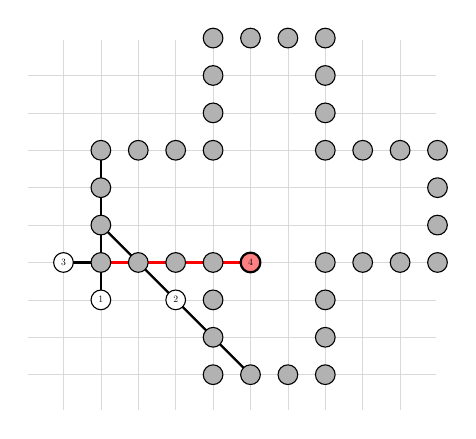
\begin{tikzpicture}[scale=0.95]
\draw[step=2*\unitsize,gray!30,very thin,shift={(-\unitsize, -\unitsize)}] (-11.900000*\unitsize,-9.900000*\unitsize) grid (9.900000*\unitsize,9.900000*\unitsize);
\tikzstyle{every node}=[draw,
			circle,
			fill=white,
			minimum size  = 1*\unitsize,
			node distance = 2*\unitsize,
			inner sep=0pt
			] 


\draw[thick] (-9*\unitsize,-1*\unitsize) -- (-9*\unitsize,1*\unitsize);
    

\draw[thick] (-9*\unitsize,1*\unitsize) -- (-9*\unitsize,3*\unitsize);
    

\draw[thick] (-9*\unitsize,-1*\unitsize) -- (-9*\unitsize,-3*\unitsize);
    

\draw[thick] (-9*\unitsize,-3*\unitsize) -- (-9*\unitsize,-5*\unitsize);
    

\draw[thick] (-5*\unitsize,-5*\unitsize) -- (-3*\unitsize,-7*\unitsize);
    

\draw[thick] (-3*\unitsize,-7*\unitsize) -- (-1*\unitsize,-9*\unitsize);
    

\draw[thick] (-5*\unitsize,-5*\unitsize) -- (-7*\unitsize,-3*\unitsize);
    

\draw[thick] (-7*\unitsize,-3*\unitsize) -- (-9*\unitsize,-1*\unitsize);
    

\draw[thick] (-7*\unitsize,-3*\unitsize) -- (-5*\unitsize,-3*\unitsize);
    

\draw[thick] (-5*\unitsize,-3*\unitsize) -- (-3*\unitsize,-3*\unitsize);
    

\draw[thick] (-7*\unitsize,-3*\unitsize) -- (-9*\unitsize,-3*\unitsize);
    

\draw[thick] (-9*\unitsize,-3*\unitsize) -- (-11*\unitsize,-3*\unitsize);

\draw[very thick, color=red] (-1*\unitsize,-3*\unitsize) -- (-3*\unitsize,-3*\unitsize);
\draw[very thick, color=red] (-3*\unitsize,-3*\unitsize) -- (-5*\unitsize,-3*\unitsize);
\draw[very thick, color=red] (-5*\unitsize,-3*\unitsize) -- (-7*\unitsize,-3*\unitsize);
\draw[very thick, color=red] (-7*\unitsize,-3*\unitsize) -- (-9*\unitsize,-3*\unitsize);


\node[fill=black!30, thin] at (3*\unitsize,9*\unitsize) {};
        

\node[fill=black!30, thin] at (3*\unitsize,7*\unitsize) {};
        

\node[fill=black!30, thin] at (3*\unitsize,5*\unitsize) {};
        

\node[fill=black!30, thin] at (3*\unitsize,3*\unitsize) {};
        

\node[fill=black!30, thin] at (5*\unitsize,3*\unitsize) {};
        

\node[fill=black!30, thin] at (7*\unitsize,3*\unitsize) {};
        

\node[fill=black!30, thin] at (9*\unitsize,3*\unitsize) {};
        

\node[fill=black!30, thin] at (9*\unitsize,1*\unitsize) {};
        

\node[fill=black!30, thin] at (9*\unitsize,-1*\unitsize) {};
        

\node[fill=black!30, thin] at (9*\unitsize,-3*\unitsize) {};
        

\node[fill=black!30, thin] at (7*\unitsize,-3*\unitsize) {};
        

\node[fill=black!30, thin] at (5*\unitsize,-3*\unitsize) {};
        

\node[fill=black!30, thin] at (3*\unitsize,-3*\unitsize) {};
        

\node[fill=black!30, thin] at (3*\unitsize,-5*\unitsize) {};
        

\node[fill=black!30, thin] at (3*\unitsize,-7*\unitsize) {};
        

\node[fill=black!30, thin] at (3*\unitsize,-9*\unitsize) {};
        

\node[fill=black!30, thin] at (1*\unitsize,-9*\unitsize) {};
        

\node[fill=black!30, thin] at (-1*\unitsize,-9*\unitsize) {};
        

\node[fill=black!30, thin] at (-3*\unitsize,-9*\unitsize) {};
        

\node[fill=black!30, thin] at (-3*\unitsize,-7*\unitsize) {};
        

\node[fill=black!30, thin] at (-3*\unitsize,-5*\unitsize) {};
        

\node[fill=black!30, thin] at (-3*\unitsize,-3*\unitsize) {};
        

\node[fill=black!30, thin] at (-5*\unitsize,-3*\unitsize) {};
        

\node[fill=black!30, thin] at (-7*\unitsize,-3*\unitsize) {};
        

\node[fill=black!30, thin] at (-9*\unitsize,-3*\unitsize) {};
        

\node[fill=black!30, thin] at (-9*\unitsize,-1*\unitsize) {};
        

\node[fill=black!30, thin] at (-9*\unitsize,1*\unitsize) {};
        

\node[fill=black!30, thin] at (-9*\unitsize,3*\unitsize) {};
        

\node[fill=black!30, thin] at (-7*\unitsize,3*\unitsize) {};
        

\node[fill=black!30, thin] at (-5*\unitsize,3*\unitsize) {};
        

\node[fill=black!30, thin] at (-3*\unitsize,3*\unitsize) {};
        

\node[fill=black!30, thin] at (-3*\unitsize,5*\unitsize) {};
        

\node[fill=black!30, thin] at (-3*\unitsize,7*\unitsize) {};
        

\node[fill=black!30, thin] at (-3*\unitsize,9*\unitsize) {};
        

\node[fill=black!30, thin] at (-1*\unitsize,9*\unitsize) {};
        

\node[fill=black!30, thin] at (1*\unitsize,9*\unitsize) {};
        

\node[thin] at (-9*\unitsize,-5*\unitsize)  {\scalebox{0.35}{1}};
        

\node[thin] at (-5*\unitsize,-5*\unitsize)  {\scalebox{0.35}{2}};
        

\node[thin] at (-11*\unitsize,-3*\unitsize)  {\scalebox{0.35}{3}};
        
\node[thick, fill=red!50] at (-1*\unitsize,-3*\unitsize) {\scalebox{0.35}{4}};

\end{tikzpicture}



Moves may not overlap.
\end{center}
\end{frame}

\begin{frame}
\frametitle{The goal}

{\bf The goal is to find the longest sequence of moves.}

\vspace{5mm}
Example of shortest possible sequence (20 moves):

\vspace{3mm}
\begin{center}
\includegraphics[height=4cm]{positions/morpionmini.jpg}
\end{center}
\begin{flushright}
\footnotesize Ch. Boyer, \url{morpionsolitaire.com}
\end{flushright}
\end{frame}

\subsection{Bounds}

\begin{frame}
\frametitle{Record sequence of Bruneau (170 moves, 1974)}
\vspace*{-5mm}
\begin{center}

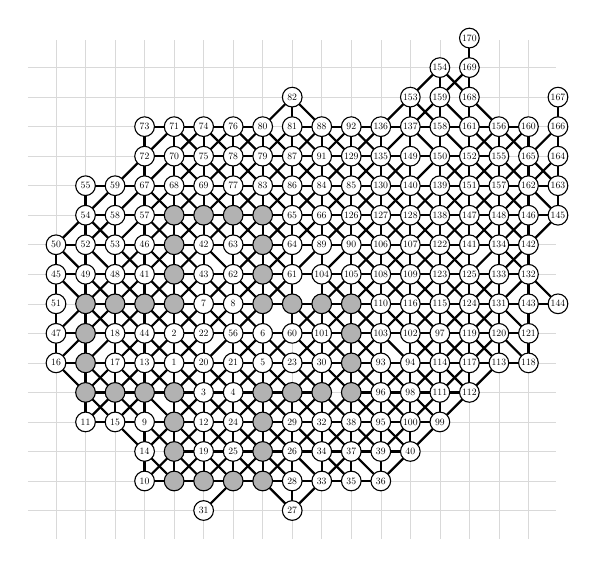
\begin{tikzpicture}[scale=0.75]
\draw[step=2*\unitsize,gray!30,very thin,shift={(-\unitsize, -\unitsize)}] (-11.900000*\unitsize,-11.900000*\unitsize) grid (23.900000*\unitsize,21.900000*\unitsize);
\tikzstyle{every node}=[draw,
			circle,
			fill=white,
			minimum size  = 1*\unitsize,
			node distance = 2*\unitsize,
			inner sep=0pt
			] 


\draw[thick] (-3*\unitsize,-5*\unitsize) -- (-3*\unitsize,-3*\unitsize);
    

\draw[thick] (-3*\unitsize,-3*\unitsize) -- (-3*\unitsize,-1*\unitsize);
    

\draw[thick] (-3*\unitsize,-5*\unitsize) -- (-3*\unitsize,-7*\unitsize);
    

\draw[thick] (-3*\unitsize,-7*\unitsize) -- (-3*\unitsize,-9*\unitsize);
    

\draw[thick] (-3*\unitsize,3*\unitsize) -- (-3*\unitsize,5*\unitsize);
    

\draw[thick] (-3*\unitsize,5*\unitsize) -- (-3*\unitsize,7*\unitsize);
    

\draw[thick] (-3*\unitsize,3*\unitsize) -- (-3*\unitsize,1*\unitsize);
    

\draw[thick] (-3*\unitsize,1*\unitsize) -- (-3*\unitsize,-1*\unitsize);
    

\draw[thick] (-5*\unitsize,-3*\unitsize) -- (-3*\unitsize,-3*\unitsize);
    

\draw[thick] (-3*\unitsize,-3*\unitsize) -- (-1*\unitsize,-3*\unitsize);
    

\draw[thick] (-5*\unitsize,-3*\unitsize) -- (-7*\unitsize,-3*\unitsize);
    

\draw[thick] (-7*\unitsize,-3*\unitsize) -- (-9*\unitsize,-3*\unitsize);
    

\draw[thick] (3*\unitsize,-3*\unitsize) -- (5*\unitsize,-3*\unitsize);
    

\draw[thick] (5*\unitsize,-3*\unitsize) -- (7*\unitsize,-3*\unitsize);
    

\draw[thick] (3*\unitsize,-3*\unitsize) -- (1*\unitsize,-3*\unitsize);
    

\draw[thick] (1*\unitsize,-3*\unitsize) -- (-1*\unitsize,-3*\unitsize);
    

\draw[thick] (3*\unitsize,-5*\unitsize) -- (3*\unitsize,-3*\unitsize);
    

\draw[thick] (3*\unitsize,-3*\unitsize) -- (3*\unitsize,-1*\unitsize);
    

\draw[thick] (3*\unitsize,-5*\unitsize) -- (3*\unitsize,-7*\unitsize);
    

\draw[thick] (3*\unitsize,-7*\unitsize) -- (3*\unitsize,-9*\unitsize);
    

\draw[thick] (3*\unitsize,3*\unitsize) -- (3*\unitsize,5*\unitsize);
    

\draw[thick] (3*\unitsize,5*\unitsize) -- (3*\unitsize,7*\unitsize);
    

\draw[thick] (3*\unitsize,3*\unitsize) -- (3*\unitsize,1*\unitsize);
    

\draw[thick] (3*\unitsize,1*\unitsize) -- (3*\unitsize,-1*\unitsize);
    

\draw[thick] (-5*\unitsize,3*\unitsize) -- (-3*\unitsize,3*\unitsize);
    

\draw[thick] (-3*\unitsize,3*\unitsize) -- (-1*\unitsize,3*\unitsize);
    

\draw[thick] (-5*\unitsize,3*\unitsize) -- (-7*\unitsize,3*\unitsize);
    

\draw[thick] (-7*\unitsize,3*\unitsize) -- (-9*\unitsize,3*\unitsize);
    

\draw[thick] (3*\unitsize,3*\unitsize) -- (5*\unitsize,3*\unitsize);
    

\draw[thick] (5*\unitsize,3*\unitsize) -- (7*\unitsize,3*\unitsize);
    

\draw[thick] (3*\unitsize,3*\unitsize) -- (1*\unitsize,3*\unitsize);
    

\draw[thick] (1*\unitsize,3*\unitsize) -- (-1*\unitsize,3*\unitsize);
    

\draw[thick] (-5*\unitsize,-5*\unitsize) -- (-3*\unitsize,-7*\unitsize);
    

\draw[thick] (-3*\unitsize,-7*\unitsize) -- (-1*\unitsize,-9*\unitsize);
    

\draw[thick] (-5*\unitsize,-5*\unitsize) -- (-7*\unitsize,-3*\unitsize);
    

\draw[thick] (-7*\unitsize,-3*\unitsize) -- (-9*\unitsize,-1*\unitsize);
    

\draw[thick] (-1*\unitsize,-9*\unitsize) -- (1*\unitsize,-9*\unitsize);
    

\draw[thick] (1*\unitsize,-9*\unitsize) -- (3*\unitsize,-9*\unitsize);
    

\draw[thick] (-1*\unitsize,-9*\unitsize) -- (-3*\unitsize,-9*\unitsize);
    

\draw[thick] (-3*\unitsize,-9*\unitsize) -- (-5*\unitsize,-9*\unitsize);
    

\draw[thick] (-9*\unitsize,-1*\unitsize) -- (-9*\unitsize,1*\unitsize);
    

\draw[thick] (-9*\unitsize,1*\unitsize) -- (-9*\unitsize,3*\unitsize);
    

\draw[thick] (-9*\unitsize,-1*\unitsize) -- (-9*\unitsize,-3*\unitsize);
    

\draw[thick] (-9*\unitsize,-3*\unitsize) -- (-9*\unitsize,-5*\unitsize);
    

\draw[thick] (-1*\unitsize,-5*\unitsize) -- (1*\unitsize,-3*\unitsize);
    

\draw[thick] (1*\unitsize,-3*\unitsize) -- (3*\unitsize,-1*\unitsize);
    

\draw[thick] (-1*\unitsize,-5*\unitsize) -- (-3*\unitsize,-7*\unitsize);
    

\draw[thick] (-3*\unitsize,-7*\unitsize) -- (-5*\unitsize,-9*\unitsize);
    

\draw[thick] (-5*\unitsize,-1*\unitsize) -- (-3*\unitsize,1*\unitsize);
    

\draw[thick] (-3*\unitsize,1*\unitsize) -- (-1*\unitsize,3*\unitsize);
    

\draw[thick] (-5*\unitsize,-1*\unitsize) -- (-7*\unitsize,-3*\unitsize);
    

\draw[thick] (-7*\unitsize,-3*\unitsize) -- (-9*\unitsize,-5*\unitsize);
    

\draw[thick] (-5*\unitsize,-5*\unitsize) -- (-5*\unitsize,-3*\unitsize);
    

\draw[thick] (-5*\unitsize,-3*\unitsize) -- (-5*\unitsize,-1*\unitsize);
    

\draw[thick] (-5*\unitsize,-5*\unitsize) -- (-5*\unitsize,-7*\unitsize);
    

\draw[thick] (-5*\unitsize,-7*\unitsize) -- (-5*\unitsize,-9*\unitsize);
    

\draw[thick] (-5*\unitsize,-5*\unitsize) -- (-3*\unitsize,-5*\unitsize);
    

\draw[thick] (-3*\unitsize,-5*\unitsize) -- (-1*\unitsize,-5*\unitsize);
    

\draw[thick] (-5*\unitsize,-5*\unitsize) -- (-7*\unitsize,-5*\unitsize);
    

\draw[thick] (-7*\unitsize,-5*\unitsize) -- (-9*\unitsize,-5*\unitsize);
    

\draw[thick] (-7*\unitsize,-5*\unitsize) -- (-5*\unitsize,-7*\unitsize);
    

\draw[thick] (-5*\unitsize,-7*\unitsize) -- (-3*\unitsize,-9*\unitsize);
    

\draw[thick] (-7*\unitsize,-5*\unitsize) -- (-9*\unitsize,-3*\unitsize);
    

\draw[thick] (-9*\unitsize,-3*\unitsize) -- (-11*\unitsize,-1*\unitsize);
    

\draw[thick] (-7*\unitsize,-1*\unitsize) -- (-5*\unitsize,-1*\unitsize);
    

\draw[thick] (-5*\unitsize,-1*\unitsize) -- (-3*\unitsize,-1*\unitsize);
    

\draw[thick] (-7*\unitsize,-1*\unitsize) -- (-9*\unitsize,-1*\unitsize);
    

\draw[thick] (-9*\unitsize,-1*\unitsize) -- (-11*\unitsize,-1*\unitsize);
    

\draw[thick] (-7*\unitsize,-1*\unitsize) -- (-7*\unitsize,1*\unitsize);
    

\draw[thick] (-7*\unitsize,1*\unitsize) -- (-7*\unitsize,3*\unitsize);
    

\draw[thick] (-7*\unitsize,-1*\unitsize) -- (-7*\unitsize,-3*\unitsize);
    

\draw[thick] (-7*\unitsize,-3*\unitsize) -- (-7*\unitsize,-5*\unitsize);
    

\draw[thick] (-3*\unitsize,-5*\unitsize) -- (-1*\unitsize,-7*\unitsize);
    

\draw[thick] (-1*\unitsize,-7*\unitsize) -- (1*\unitsize,-9*\unitsize);
    

\draw[thick] (-3*\unitsize,-5*\unitsize) -- (-5*\unitsize,-3*\unitsize);
    

\draw[thick] (-5*\unitsize,-3*\unitsize) -- (-7*\unitsize,-1*\unitsize);
    

\draw[thick] (-1*\unitsize,-5*\unitsize) -- (-1*\unitsize,-3*\unitsize);
    

\draw[thick] (-1*\unitsize,-3*\unitsize) -- (-1*\unitsize,-1*\unitsize);
    

\draw[thick] (-1*\unitsize,-5*\unitsize) -- (-1*\unitsize,-7*\unitsize);
    

\draw[thick] (-1*\unitsize,-7*\unitsize) -- (-1*\unitsize,-9*\unitsize);
    

\draw[thick] (-1*\unitsize,-3*\unitsize) -- (1*\unitsize,-1*\unitsize);
    

\draw[thick] (1*\unitsize,-1*\unitsize) -- (3*\unitsize,1*\unitsize);
    

\draw[thick] (-1*\unitsize,-3*\unitsize) -- (-3*\unitsize,-5*\unitsize);
    

\draw[thick] (-3*\unitsize,-5*\unitsize) -- (-5*\unitsize,-7*\unitsize);
    

\draw[thick] (-3*\unitsize,-1*\unitsize) -- (-1*\unitsize,1*\unitsize);
    

\draw[thick] (-1*\unitsize,1*\unitsize) -- (1*\unitsize,3*\unitsize);
    

\draw[thick] (-3*\unitsize,-1*\unitsize) -- (-5*\unitsize,-3*\unitsize);
    

\draw[thick] (-5*\unitsize,-3*\unitsize) -- (-7*\unitsize,-5*\unitsize);
    

\draw[thick] (1*\unitsize,-1*\unitsize) -- (3*\unitsize,-1*\unitsize);
    

\draw[thick] (3*\unitsize,-1*\unitsize) -- (5*\unitsize,-1*\unitsize);
    

\draw[thick] (1*\unitsize,-1*\unitsize) -- (-1*\unitsize,-1*\unitsize);
    

\draw[thick] (-1*\unitsize,-1*\unitsize) -- (-3*\unitsize,-1*\unitsize);
    

\draw[thick] (1*\unitsize,-5*\unitsize) -- (3*\unitsize,-3*\unitsize);
    

\draw[thick] (3*\unitsize,-3*\unitsize) -- (5*\unitsize,-1*\unitsize);
    

\draw[thick] (1*\unitsize,-5*\unitsize) -- (-1*\unitsize,-7*\unitsize);
    

\draw[thick] (-1*\unitsize,-7*\unitsize) -- (-3*\unitsize,-9*\unitsize);
    

\draw[thick] (1*\unitsize,-5*\unitsize) -- (1*\unitsize,-3*\unitsize);
    

\draw[thick] (1*\unitsize,-3*\unitsize) -- (1*\unitsize,-1*\unitsize);
    

\draw[thick] (1*\unitsize,-5*\unitsize) -- (1*\unitsize,-7*\unitsize);
    

\draw[thick] (1*\unitsize,-7*\unitsize) -- (1*\unitsize,-9*\unitsize);
    

\draw[thick] (1*\unitsize,-7*\unitsize) -- (3*\unitsize,-7*\unitsize);
    

\draw[thick] (3*\unitsize,-7*\unitsize) -- (5*\unitsize,-7*\unitsize);
    

\draw[thick] (1*\unitsize,-7*\unitsize) -- (-1*\unitsize,-7*\unitsize);
    

\draw[thick] (-1*\unitsize,-7*\unitsize) -- (-3*\unitsize,-7*\unitsize);
    

\draw[thick] (1*\unitsize,-7*\unitsize) -- (3*\unitsize,-9*\unitsize);
    

\draw[thick] (3*\unitsize,-9*\unitsize) -- (5*\unitsize,-11*\unitsize);
    

\draw[thick] (1*\unitsize,-7*\unitsize) -- (-1*\unitsize,-5*\unitsize);
    

\draw[thick] (-1*\unitsize,-5*\unitsize) -- (-3*\unitsize,-3*\unitsize);
    

\draw[thick] (1*\unitsize,-5*\unitsize) -- (3*\unitsize,-7*\unitsize);
    

\draw[thick] (3*\unitsize,-7*\unitsize) -- (5*\unitsize,-9*\unitsize);
    

\draw[thick] (1*\unitsize,-5*\unitsize) -- (-1*\unitsize,-3*\unitsize);
    

\draw[thick] (-1*\unitsize,-3*\unitsize) -- (-3*\unitsize,-1*\unitsize);
    

\draw[thick] (5*\unitsize,-7*\unitsize) -- (5*\unitsize,-5*\unitsize);
    

\draw[thick] (5*\unitsize,-5*\unitsize) -- (5*\unitsize,-3*\unitsize);
    

\draw[thick] (5*\unitsize,-7*\unitsize) -- (5*\unitsize,-9*\unitsize);
    

\draw[thick] (5*\unitsize,-9*\unitsize) -- (5*\unitsize,-11*\unitsize);
    

\draw[thick] (3*\unitsize,-5*\unitsize) -- (5*\unitsize,-3*\unitsize);
    

\draw[thick] (5*\unitsize,-3*\unitsize) -- (7*\unitsize,-1*\unitsize);
    

\draw[thick] (3*\unitsize,-5*\unitsize) -- (1*\unitsize,-7*\unitsize);
    

\draw[thick] (1*\unitsize,-7*\unitsize) -- (-1*\unitsize,-9*\unitsize);
    

\draw[thick] (3*\unitsize,-7*\unitsize) -- (5*\unitsize,-5*\unitsize);
    

\draw[thick] (5*\unitsize,-5*\unitsize) -- (7*\unitsize,-3*\unitsize);
    

\draw[thick] (3*\unitsize,-7*\unitsize) -- (1*\unitsize,-9*\unitsize);
    

\draw[thick] (1*\unitsize,-9*\unitsize) -- (-1*\unitsize,-11*\unitsize);
    

\draw[thick] (3*\unitsize,-5*\unitsize) -- (5*\unitsize,-5*\unitsize);
    

\draw[thick] (5*\unitsize,-5*\unitsize) -- (7*\unitsize,-5*\unitsize);
    

\draw[thick] (3*\unitsize,-5*\unitsize) -- (1*\unitsize,-5*\unitsize);
    

\draw[thick] (1*\unitsize,-5*\unitsize) -- (-1*\unitsize,-5*\unitsize);
    

\draw[thick] (3*\unitsize,-5*\unitsize) -- (5*\unitsize,-7*\unitsize);
    

\draw[thick] (5*\unitsize,-7*\unitsize) -- (7*\unitsize,-9*\unitsize);
    

\draw[thick] (3*\unitsize,-5*\unitsize) -- (1*\unitsize,-3*\unitsize);
    

\draw[thick] (1*\unitsize,-3*\unitsize) -- (-1*\unitsize,-1*\unitsize);
    

\draw[thick] (7*\unitsize,-5*\unitsize) -- (7*\unitsize,-3*\unitsize);
    

\draw[thick] (7*\unitsize,-3*\unitsize) -- (7*\unitsize,-1*\unitsize);
    

\draw[thick] (7*\unitsize,-5*\unitsize) -- (7*\unitsize,-7*\unitsize);
    

\draw[thick] (7*\unitsize,-7*\unitsize) -- (7*\unitsize,-9*\unitsize);
    

\draw[thick] (5*\unitsize,-5*\unitsize) -- (7*\unitsize,-7*\unitsize);
    

\draw[thick] (7*\unitsize,-7*\unitsize) -- (9*\unitsize,-9*\unitsize);
    

\draw[thick] (5*\unitsize,-5*\unitsize) -- (3*\unitsize,-3*\unitsize);
    

\draw[thick] (3*\unitsize,-3*\unitsize) -- (1*\unitsize,-1*\unitsize);
    

\draw[thick] (7*\unitsize,-9*\unitsize) -- (9*\unitsize,-9*\unitsize);
    

\draw[thick] (9*\unitsize,-9*\unitsize) -- (11*\unitsize,-9*\unitsize);
    

\draw[thick] (7*\unitsize,-9*\unitsize) -- (5*\unitsize,-9*\unitsize);
    

\draw[thick] (5*\unitsize,-9*\unitsize) -- (3*\unitsize,-9*\unitsize);
    

\draw[thick] (7*\unitsize,-5*\unitsize) -- (9*\unitsize,-7*\unitsize);
    

\draw[thick] (9*\unitsize,-7*\unitsize) -- (11*\unitsize,-9*\unitsize);
    

\draw[thick] (7*\unitsize,-5*\unitsize) -- (5*\unitsize,-3*\unitsize);
    

\draw[thick] (5*\unitsize,-3*\unitsize) -- (3*\unitsize,-1*\unitsize);
    

\draw[thick] (9*\unitsize,-5*\unitsize) -- (9*\unitsize,-3*\unitsize);
    

\draw[thick] (9*\unitsize,-3*\unitsize) -- (9*\unitsize,-1*\unitsize);
    

\draw[thick] (9*\unitsize,-5*\unitsize) -- (9*\unitsize,-7*\unitsize);
    

\draw[thick] (9*\unitsize,-7*\unitsize) -- (9*\unitsize,-9*\unitsize);
    

\draw[thick] (7*\unitsize,-3*\unitsize) -- (9*\unitsize,-5*\unitsize);
    

\draw[thick] (9*\unitsize,-5*\unitsize) -- (11*\unitsize,-7*\unitsize);
    

\draw[thick] (7*\unitsize,-3*\unitsize) -- (5*\unitsize,-1*\unitsize);
    

\draw[thick] (5*\unitsize,-1*\unitsize) -- (3*\unitsize,1*\unitsize);
    

\draw[thick] (9*\unitsize,-7*\unitsize) -- (11*\unitsize,-7*\unitsize);
    

\draw[thick] (11*\unitsize,-7*\unitsize) -- (13*\unitsize,-7*\unitsize);
    

\draw[thick] (9*\unitsize,-7*\unitsize) -- (7*\unitsize,-7*\unitsize);
    

\draw[thick] (7*\unitsize,-7*\unitsize) -- (5*\unitsize,-7*\unitsize);
    

\draw[thick] (-7*\unitsize,3*\unitsize) -- (-5*\unitsize,5*\unitsize);
    

\draw[thick] (-5*\unitsize,5*\unitsize) -- (-3*\unitsize,7*\unitsize);
    

\draw[thick] (-7*\unitsize,3*\unitsize) -- (-9*\unitsize,1*\unitsize);
    

\draw[thick] (-9*\unitsize,1*\unitsize) -- (-11*\unitsize,-1*\unitsize);
    

\draw[thick] (-5*\unitsize,3*\unitsize) -- (-3*\unitsize,5*\unitsize);
    

\draw[thick] (-3*\unitsize,5*\unitsize) -- (-1*\unitsize,7*\unitsize);
    

\draw[thick] (-5*\unitsize,3*\unitsize) -- (-7*\unitsize,1*\unitsize);
    

\draw[thick] (-7*\unitsize,1*\unitsize) -- (-9*\unitsize,-1*\unitsize);
    

\draw[thick] (-1*\unitsize,3*\unitsize) -- (-1*\unitsize,5*\unitsize);
    

\draw[thick] (-1*\unitsize,5*\unitsize) -- (-1*\unitsize,7*\unitsize);
    

\draw[thick] (-1*\unitsize,3*\unitsize) -- (-1*\unitsize,1*\unitsize);
    

\draw[thick] (-1*\unitsize,1*\unitsize) -- (-1*\unitsize,-1*\unitsize);
    

\draw[thick] (-5*\unitsize,1*\unitsize) -- (-3*\unitsize,3*\unitsize);
    

\draw[thick] (-3*\unitsize,3*\unitsize) -- (-1*\unitsize,5*\unitsize);
    

\draw[thick] (-5*\unitsize,1*\unitsize) -- (-7*\unitsize,-1*\unitsize);
    

\draw[thick] (-7*\unitsize,-1*\unitsize) -- (-9*\unitsize,-3*\unitsize);
    

\draw[thick] (-7*\unitsize,1*\unitsize) -- (-5*\unitsize,-1*\unitsize);
    

\draw[thick] (-5*\unitsize,-1*\unitsize) -- (-3*\unitsize,-3*\unitsize);
    

\draw[thick] (-7*\unitsize,1*\unitsize) -- (-9*\unitsize,3*\unitsize);
    

\draw[thick] (-9*\unitsize,3*\unitsize) -- (-11*\unitsize,5*\unitsize);
    

\draw[thick] (-5*\unitsize,3*\unitsize) -- (-5*\unitsize,5*\unitsize);
    

\draw[thick] (-5*\unitsize,5*\unitsize) -- (-5*\unitsize,7*\unitsize);
    

\draw[thick] (-5*\unitsize,3*\unitsize) -- (-5*\unitsize,1*\unitsize);
    

\draw[thick] (-5*\unitsize,1*\unitsize) -- (-5*\unitsize,-1*\unitsize);
    

\draw[thick] (-7*\unitsize,1*\unitsize) -- (-5*\unitsize,1*\unitsize);
    

\draw[thick] (-5*\unitsize,1*\unitsize) -- (-3*\unitsize,1*\unitsize);
    

\draw[thick] (-7*\unitsize,1*\unitsize) -- (-9*\unitsize,1*\unitsize);
    

\draw[thick] (-9*\unitsize,1*\unitsize) -- (-11*\unitsize,1*\unitsize);
    

\draw[thick] (-7*\unitsize,5*\unitsize) -- (-5*\unitsize,7*\unitsize);
    

\draw[thick] (-5*\unitsize,7*\unitsize) -- (-3*\unitsize,9*\unitsize);
    

\draw[thick] (-7*\unitsize,5*\unitsize) -- (-9*\unitsize,3*\unitsize);
    

\draw[thick] (-9*\unitsize,3*\unitsize) -- (-11*\unitsize,1*\unitsize);
    

\draw[thick] (-7*\unitsize,5*\unitsize) -- (-5*\unitsize,5*\unitsize);
    

\draw[thick] (-5*\unitsize,5*\unitsize) -- (-3*\unitsize,5*\unitsize);
    

\draw[thick] (-7*\unitsize,5*\unitsize) -- (-9*\unitsize,5*\unitsize);
    

\draw[thick] (-9*\unitsize,5*\unitsize) -- (-11*\unitsize,5*\unitsize);
    

\draw[thick] (-7*\unitsize,3*\unitsize) -- (-5*\unitsize,1*\unitsize);
    

\draw[thick] (-5*\unitsize,1*\unitsize) -- (-3*\unitsize,-1*\unitsize);
    

\draw[thick] (-7*\unitsize,3*\unitsize) -- (-9*\unitsize,5*\unitsize);
    

\draw[thick] (-9*\unitsize,5*\unitsize) -- (-11*\unitsize,7*\unitsize);
    

\draw[thick] (-11*\unitsize,3*\unitsize) -- (-11*\unitsize,5*\unitsize);
    

\draw[thick] (-11*\unitsize,5*\unitsize) -- (-11*\unitsize,7*\unitsize);
    

\draw[thick] (-11*\unitsize,3*\unitsize) -- (-11*\unitsize,1*\unitsize);
    

\draw[thick] (-11*\unitsize,1*\unitsize) -- (-11*\unitsize,-1*\unitsize);
    

\draw[thick] (-5*\unitsize,3*\unitsize) -- (-3*\unitsize,1*\unitsize);
    

\draw[thick] (-3*\unitsize,1*\unitsize) -- (-1*\unitsize,-1*\unitsize);
    

\draw[thick] (-5*\unitsize,3*\unitsize) -- (-7*\unitsize,5*\unitsize);
    

\draw[thick] (-7*\unitsize,5*\unitsize) -- (-9*\unitsize,7*\unitsize);
    

\draw[thick] (-7*\unitsize,7*\unitsize) -- (-5*\unitsize,7*\unitsize);
    

\draw[thick] (-5*\unitsize,7*\unitsize) -- (-3*\unitsize,7*\unitsize);
    

\draw[thick] (-7*\unitsize,7*\unitsize) -- (-9*\unitsize,7*\unitsize);
    

\draw[thick] (-9*\unitsize,7*\unitsize) -- (-11*\unitsize,7*\unitsize);
    

\draw[thick] (-5*\unitsize,5*\unitsize) -- (-3*\unitsize,3*\unitsize);
    

\draw[thick] (-3*\unitsize,3*\unitsize) -- (-1*\unitsize,1*\unitsize);
    

\draw[thick] (-5*\unitsize,5*\unitsize) -- (-7*\unitsize,7*\unitsize);
    

\draw[thick] (-7*\unitsize,7*\unitsize) -- (-9*\unitsize,9*\unitsize);
    

\draw[thick] (-9*\unitsize,7*\unitsize) -- (-9*\unitsize,9*\unitsize);
    

\draw[thick] (-9*\unitsize,9*\unitsize) -- (-9*\unitsize,11*\unitsize);
    

\draw[thick] (-9*\unitsize,7*\unitsize) -- (-9*\unitsize,5*\unitsize);
    

\draw[thick] (-9*\unitsize,5*\unitsize) -- (-9*\unitsize,3*\unitsize);
    

\draw[thick] (-1*\unitsize,3*\unitsize) -- (1*\unitsize,1*\unitsize);
    

\draw[thick] (1*\unitsize,1*\unitsize) -- (3*\unitsize,-1*\unitsize);
    

\draw[thick] (-1*\unitsize,3*\unitsize) -- (-3*\unitsize,5*\unitsize);
    

\draw[thick] (-3*\unitsize,5*\unitsize) -- (-5*\unitsize,7*\unitsize);
    

\draw[thick] (-1*\unitsize,5*\unitsize) -- (1*\unitsize,3*\unitsize);
    

\draw[thick] (1*\unitsize,3*\unitsize) -- (3*\unitsize,1*\unitsize);
    

\draw[thick] (-1*\unitsize,5*\unitsize) -- (-3*\unitsize,7*\unitsize);
    

\draw[thick] (-3*\unitsize,7*\unitsize) -- (-5*\unitsize,9*\unitsize);
    

\draw[thick] (-5*\unitsize,9*\unitsize) -- (-3*\unitsize,9*\unitsize);
    

\draw[thick] (-3*\unitsize,9*\unitsize) -- (-1*\unitsize,9*\unitsize);
    

\draw[thick] (-5*\unitsize,9*\unitsize) -- (-7*\unitsize,9*\unitsize);
    

\draw[thick] (-7*\unitsize,9*\unitsize) -- (-9*\unitsize,9*\unitsize);
    

\draw[thick] (-7*\unitsize,7*\unitsize) -- (-7*\unitsize,9*\unitsize);
    

\draw[thick] (-7*\unitsize,9*\unitsize) -- (-7*\unitsize,11*\unitsize);
    

\draw[thick] (-7*\unitsize,7*\unitsize) -- (-7*\unitsize,5*\unitsize);
    

\draw[thick] (-7*\unitsize,5*\unitsize) -- (-7*\unitsize,3*\unitsize);
    

\draw[thick] (1*\unitsize,1*\unitsize) -- (3*\unitsize,1*\unitsize);
    

\draw[thick] (3*\unitsize,1*\unitsize) -- (5*\unitsize,1*\unitsize);
    

\draw[thick] (1*\unitsize,1*\unitsize) -- (-1*\unitsize,1*\unitsize);
    

\draw[thick] (-1*\unitsize,1*\unitsize) -- (-3*\unitsize,1*\unitsize);
    

\draw[thick] (1*\unitsize,1*\unitsize) -- (3*\unitsize,3*\unitsize);
    

\draw[thick] (3*\unitsize,3*\unitsize) -- (5*\unitsize,5*\unitsize);
    

\draw[thick] (1*\unitsize,1*\unitsize) -- (-1*\unitsize,-1*\unitsize);
    

\draw[thick] (-1*\unitsize,-1*\unitsize) -- (-3*\unitsize,-3*\unitsize);
    

\draw[thick] (1*\unitsize,5*\unitsize) -- (3*\unitsize,5*\unitsize);
    

\draw[thick] (3*\unitsize,5*\unitsize) -- (5*\unitsize,5*\unitsize);
    

\draw[thick] (1*\unitsize,5*\unitsize) -- (-1*\unitsize,5*\unitsize);
    

\draw[thick] (-1*\unitsize,5*\unitsize) -- (-3*\unitsize,5*\unitsize);
    

\draw[thick] (1*\unitsize,3*\unitsize) -- (1*\unitsize,5*\unitsize);
    

\draw[thick] (1*\unitsize,5*\unitsize) -- (1*\unitsize,7*\unitsize);
    

\draw[thick] (1*\unitsize,3*\unitsize) -- (1*\unitsize,1*\unitsize);
    

\draw[thick] (1*\unitsize,1*\unitsize) -- (1*\unitsize,-1*\unitsize);
    

\draw[thick] (1*\unitsize,7*\unitsize) -- (3*\unitsize,7*\unitsize);
    

\draw[thick] (3*\unitsize,7*\unitsize) -- (5*\unitsize,7*\unitsize);
    

\draw[thick] (1*\unitsize,7*\unitsize) -- (-1*\unitsize,7*\unitsize);
    

\draw[thick] (-1*\unitsize,7*\unitsize) -- (-3*\unitsize,7*\unitsize);
    

\draw[thick] (5*\unitsize,5*\unitsize) -- (5*\unitsize,7*\unitsize);
    

\draw[thick] (5*\unitsize,7*\unitsize) -- (5*\unitsize,9*\unitsize);
    

\draw[thick] (5*\unitsize,5*\unitsize) -- (5*\unitsize,3*\unitsize);
    

\draw[thick] (5*\unitsize,3*\unitsize) -- (5*\unitsize,1*\unitsize);
    

\draw[thick] (3*\unitsize,9*\unitsize) -- (5*\unitsize,9*\unitsize);
    

\draw[thick] (5*\unitsize,9*\unitsize) -- (7*\unitsize,9*\unitsize);
    

\draw[thick] (3*\unitsize,9*\unitsize) -- (1*\unitsize,9*\unitsize);
    

\draw[thick] (1*\unitsize,9*\unitsize) -- (-1*\unitsize,9*\unitsize);
    

\draw[thick] (-1*\unitsize,7*\unitsize) -- (1*\unitsize,5*\unitsize);
    

\draw[thick] (1*\unitsize,5*\unitsize) -- (3*\unitsize,3*\unitsize);
    

\draw[thick] (-1*\unitsize,7*\unitsize) -- (-3*\unitsize,9*\unitsize);
    

\draw[thick] (-3*\unitsize,9*\unitsize) -- (-5*\unitsize,11*\unitsize);
    

\draw[thick] (1*\unitsize,7*\unitsize) -- (3*\unitsize,5*\unitsize);
    

\draw[thick] (3*\unitsize,5*\unitsize) -- (5*\unitsize,3*\unitsize);
    

\draw[thick] (1*\unitsize,7*\unitsize) -- (-1*\unitsize,9*\unitsize);
    

\draw[thick] (-1*\unitsize,9*\unitsize) -- (-3*\unitsize,11*\unitsize);
    

\draw[thick] (-5*\unitsize,11*\unitsize) -- (-3*\unitsize,11*\unitsize);
    

\draw[thick] (-3*\unitsize,11*\unitsize) -- (-1*\unitsize,11*\unitsize);
    

\draw[thick] (-5*\unitsize,11*\unitsize) -- (-7*\unitsize,11*\unitsize);
    

\draw[thick] (-7*\unitsize,11*\unitsize) -- (-9*\unitsize,11*\unitsize);
    

\draw[thick] (1*\unitsize,9*\unitsize) -- (3*\unitsize,7*\unitsize);
    

\draw[thick] (3*\unitsize,7*\unitsize) -- (5*\unitsize,5*\unitsize);
    

\draw[thick] (1*\unitsize,9*\unitsize) -- (-1*\unitsize,11*\unitsize);
    

\draw[thick] (-1*\unitsize,11*\unitsize) -- (-3*\unitsize,13*\unitsize);
    

\draw[thick] (-3*\unitsize,11*\unitsize) -- (-3*\unitsize,13*\unitsize);
    

\draw[thick] (-3*\unitsize,13*\unitsize) -- (-3*\unitsize,15*\unitsize);
    

\draw[thick] (-3*\unitsize,11*\unitsize) -- (-3*\unitsize,9*\unitsize);
    

\draw[thick] (-3*\unitsize,9*\unitsize) -- (-3*\unitsize,7*\unitsize);
    

\draw[thick] (-7*\unitsize,11*\unitsize) -- (-5*\unitsize,13*\unitsize);
    

\draw[thick] (-5*\unitsize,13*\unitsize) -- (-3*\unitsize,15*\unitsize);
    

\draw[thick] (-7*\unitsize,11*\unitsize) -- (-9*\unitsize,9*\unitsize);
    

\draw[thick] (-9*\unitsize,9*\unitsize) -- (-11*\unitsize,7*\unitsize);
    

\draw[thick] (-5*\unitsize,11*\unitsize) -- (-5*\unitsize,13*\unitsize);
    

\draw[thick] (-5*\unitsize,13*\unitsize) -- (-5*\unitsize,15*\unitsize);
    

\draw[thick] (-5*\unitsize,11*\unitsize) -- (-5*\unitsize,9*\unitsize);
    

\draw[thick] (-5*\unitsize,9*\unitsize) -- (-5*\unitsize,7*\unitsize);
    

\draw[thick] (-5*\unitsize,11*\unitsize) -- (-3*\unitsize,13*\unitsize);
    

\draw[thick] (-3*\unitsize,13*\unitsize) -- (-1*\unitsize,15*\unitsize);
    

\draw[thick] (-5*\unitsize,11*\unitsize) -- (-7*\unitsize,9*\unitsize);
    

\draw[thick] (-7*\unitsize,9*\unitsize) -- (-9*\unitsize,7*\unitsize);
    

\draw[thick] (-1*\unitsize,11*\unitsize) -- (-1*\unitsize,13*\unitsize);
    

\draw[thick] (-1*\unitsize,13*\unitsize) -- (-1*\unitsize,15*\unitsize);
    

\draw[thick] (-1*\unitsize,11*\unitsize) -- (-1*\unitsize,9*\unitsize);
    

\draw[thick] (-1*\unitsize,9*\unitsize) -- (-1*\unitsize,7*\unitsize);
    

\draw[thick] (-3*\unitsize,11*\unitsize) -- (-1*\unitsize,13*\unitsize);
    

\draw[thick] (-1*\unitsize,13*\unitsize) -- (1*\unitsize,15*\unitsize);
    

\draw[thick] (-3*\unitsize,11*\unitsize) -- (-5*\unitsize,9*\unitsize);
    

\draw[thick] (-5*\unitsize,9*\unitsize) -- (-7*\unitsize,7*\unitsize);
    

\draw[thick] (1*\unitsize,11*\unitsize) -- (3*\unitsize,9*\unitsize);
    

\draw[thick] (3*\unitsize,9*\unitsize) -- (5*\unitsize,7*\unitsize);
    

\draw[thick] (1*\unitsize,11*\unitsize) -- (-1*\unitsize,13*\unitsize);
    

\draw[thick] (-1*\unitsize,13*\unitsize) -- (-3*\unitsize,15*\unitsize);
    

\draw[thick] (1*\unitsize,11*\unitsize) -- (1*\unitsize,13*\unitsize);
    

\draw[thick] (1*\unitsize,13*\unitsize) -- (1*\unitsize,15*\unitsize);
    

\draw[thick] (1*\unitsize,11*\unitsize) -- (1*\unitsize,9*\unitsize);
    

\draw[thick] (1*\unitsize,9*\unitsize) -- (1*\unitsize,7*\unitsize);
    

\draw[thick] (-1*\unitsize,13*\unitsize) -- (1*\unitsize,13*\unitsize);
    

\draw[thick] (1*\unitsize,13*\unitsize) -- (3*\unitsize,13*\unitsize);
    

\draw[thick] (-1*\unitsize,13*\unitsize) -- (-3*\unitsize,13*\unitsize);
    

\draw[thick] (-3*\unitsize,13*\unitsize) -- (-5*\unitsize,13*\unitsize);
    

\draw[thick] (-1*\unitsize,15*\unitsize) -- (1*\unitsize,15*\unitsize);
    

\draw[thick] (1*\unitsize,15*\unitsize) -- (3*\unitsize,15*\unitsize);
    

\draw[thick] (-1*\unitsize,15*\unitsize) -- (-3*\unitsize,15*\unitsize);
    

\draw[thick] (-3*\unitsize,15*\unitsize) -- (-5*\unitsize,15*\unitsize);
    

\draw[thick] (1*\unitsize,11*\unitsize) -- (3*\unitsize,13*\unitsize);
    

\draw[thick] (3*\unitsize,13*\unitsize) -- (5*\unitsize,15*\unitsize);
    

\draw[thick] (1*\unitsize,11*\unitsize) -- (-1*\unitsize,9*\unitsize);
    

\draw[thick] (-1*\unitsize,9*\unitsize) -- (-3*\unitsize,7*\unitsize);
    

\draw[thick] (1*\unitsize,13*\unitsize) -- (3*\unitsize,15*\unitsize);
    

\draw[thick] (3*\unitsize,15*\unitsize) -- (5*\unitsize,17*\unitsize);
    

\draw[thick] (1*\unitsize,13*\unitsize) -- (-1*\unitsize,11*\unitsize);
    

\draw[thick] (-1*\unitsize,11*\unitsize) -- (-3*\unitsize,9*\unitsize);
    

\draw[thick] (3*\unitsize,11*\unitsize) -- (3*\unitsize,13*\unitsize);
    

\draw[thick] (3*\unitsize,13*\unitsize) -- (3*\unitsize,15*\unitsize);
    

\draw[thick] (3*\unitsize,11*\unitsize) -- (3*\unitsize,9*\unitsize);
    

\draw[thick] (3*\unitsize,9*\unitsize) -- (3*\unitsize,7*\unitsize);
    

\draw[thick] (3*\unitsize,7*\unitsize) -- (5*\unitsize,9*\unitsize);
    

\draw[thick] (5*\unitsize,9*\unitsize) -- (7*\unitsize,11*\unitsize);
    

\draw[thick] (3*\unitsize,7*\unitsize) -- (1*\unitsize,5*\unitsize);
    

\draw[thick] (1*\unitsize,5*\unitsize) -- (-1*\unitsize,3*\unitsize);
    

\draw[thick] (5*\unitsize,7*\unitsize) -- (7*\unitsize,9*\unitsize);
    

\draw[thick] (7*\unitsize,9*\unitsize) -- (9*\unitsize,11*\unitsize);
    

\draw[thick] (5*\unitsize,7*\unitsize) -- (3*\unitsize,5*\unitsize);
    

\draw[thick] (3*\unitsize,5*\unitsize) -- (1*\unitsize,3*\unitsize);
    

\draw[thick] (3*\unitsize,11*\unitsize) -- (5*\unitsize,11*\unitsize);
    

\draw[thick] (5*\unitsize,11*\unitsize) -- (7*\unitsize,11*\unitsize);
    

\draw[thick] (3*\unitsize,11*\unitsize) -- (1*\unitsize,11*\unitsize);
    

\draw[thick] (1*\unitsize,11*\unitsize) -- (-1*\unitsize,11*\unitsize);
    

\draw[thick] (5*\unitsize,13*\unitsize) -- (5*\unitsize,15*\unitsize);
    

\draw[thick] (5*\unitsize,15*\unitsize) -- (5*\unitsize,17*\unitsize);
    

\draw[thick] (5*\unitsize,13*\unitsize) -- (5*\unitsize,11*\unitsize);
    

\draw[thick] (5*\unitsize,11*\unitsize) -- (5*\unitsize,9*\unitsize);
    

\draw[thick] (3*\unitsize,11*\unitsize) -- (5*\unitsize,13*\unitsize);
    

\draw[thick] (5*\unitsize,13*\unitsize) -- (7*\unitsize,15*\unitsize);
    

\draw[thick] (3*\unitsize,11*\unitsize) -- (1*\unitsize,9*\unitsize);
    

\draw[thick] (1*\unitsize,9*\unitsize) -- (-1*\unitsize,7*\unitsize);
    

\draw[thick] (3*\unitsize,11*\unitsize) -- (5*\unitsize,9*\unitsize);
    

\draw[thick] (5*\unitsize,9*\unitsize) -- (7*\unitsize,7*\unitsize);
    

\draw[thick] (3*\unitsize,11*\unitsize) -- (1*\unitsize,13*\unitsize);
    

\draw[thick] (1*\unitsize,13*\unitsize) -- (-1*\unitsize,15*\unitsize);
    

\draw[thick] (5*\unitsize,11*\unitsize) -- (7*\unitsize,9*\unitsize);
    

\draw[thick] (7*\unitsize,9*\unitsize) -- (9*\unitsize,7*\unitsize);
    

\draw[thick] (5*\unitsize,11*\unitsize) -- (3*\unitsize,13*\unitsize);
    

\draw[thick] (3*\unitsize,13*\unitsize) -- (1*\unitsize,15*\unitsize);
    

\draw[thick] (7*\unitsize,11*\unitsize) -- (7*\unitsize,13*\unitsize);
    

\draw[thick] (7*\unitsize,13*\unitsize) -- (7*\unitsize,15*\unitsize);
    

\draw[thick] (7*\unitsize,11*\unitsize) -- (7*\unitsize,9*\unitsize);
    

\draw[thick] (7*\unitsize,9*\unitsize) -- (7*\unitsize,7*\unitsize);
    

\draw[thick] (5*\unitsize,11*\unitsize) -- (7*\unitsize,13*\unitsize);
    

\draw[thick] (7*\unitsize,13*\unitsize) -- (9*\unitsize,15*\unitsize);
    

\draw[thick] (5*\unitsize,11*\unitsize) -- (3*\unitsize,9*\unitsize);
    

\draw[thick] (3*\unitsize,9*\unitsize) -- (1*\unitsize,7*\unitsize);
    

\draw[thick] (7*\unitsize,-5*\unitsize) -- (9*\unitsize,-3*\unitsize);
    

\draw[thick] (9*\unitsize,-3*\unitsize) -- (11*\unitsize,-1*\unitsize);
    

\draw[thick] (7*\unitsize,-5*\unitsize) -- (5*\unitsize,-7*\unitsize);
    

\draw[thick] (5*\unitsize,-7*\unitsize) -- (3*\unitsize,-9*\unitsize);
    

\draw[thick] (9*\unitsize,-1*\unitsize) -- (11*\unitsize,-1*\unitsize);
    

\draw[thick] (11*\unitsize,-1*\unitsize) -- (13*\unitsize,-1*\unitsize);
    

\draw[thick] (9*\unitsize,-1*\unitsize) -- (7*\unitsize,-1*\unitsize);
    

\draw[thick] (7*\unitsize,-1*\unitsize) -- (5*\unitsize,-1*\unitsize);
    

\draw[thick] (9*\unitsize,-3*\unitsize) -- (11*\unitsize,-5*\unitsize);
    

\draw[thick] (11*\unitsize,-5*\unitsize) -- (13*\unitsize,-7*\unitsize);
    

\draw[thick] (9*\unitsize,-3*\unitsize) -- (7*\unitsize,-1*\unitsize);
    

\draw[thick] (7*\unitsize,-1*\unitsize) -- (5*\unitsize,1*\unitsize);
    

\draw[thick] (11*\unitsize,-5*\unitsize) -- (11*\unitsize,-3*\unitsize);
    

\draw[thick] (11*\unitsize,-3*\unitsize) -- (11*\unitsize,-1*\unitsize);
    

\draw[thick] (11*\unitsize,-5*\unitsize) -- (11*\unitsize,-7*\unitsize);
    

\draw[thick] (11*\unitsize,-7*\unitsize) -- (11*\unitsize,-9*\unitsize);
    

\draw[thick] (11*\unitsize,-3*\unitsize) -- (13*\unitsize,-1*\unitsize);
    

\draw[thick] (13*\unitsize,-1*\unitsize) -- (15*\unitsize,1*\unitsize);
    

\draw[thick] (11*\unitsize,-3*\unitsize) -- (9*\unitsize,-5*\unitsize);
    

\draw[thick] (9*\unitsize,-5*\unitsize) -- (7*\unitsize,-7*\unitsize);
    

\draw[thick] (9*\unitsize,-7*\unitsize) -- (11*\unitsize,-5*\unitsize);
    

\draw[thick] (11*\unitsize,-5*\unitsize) -- (13*\unitsize,-3*\unitsize);
    

\draw[thick] (9*\unitsize,-7*\unitsize) -- (7*\unitsize,-9*\unitsize);
    

\draw[thick] (7*\unitsize,-9*\unitsize) -- (5*\unitsize,-11*\unitsize);
    

\draw[thick] (11*\unitsize,-1*\unitsize) -- (13*\unitsize,-3*\unitsize);
    

\draw[thick] (13*\unitsize,-3*\unitsize) -- (15*\unitsize,-5*\unitsize);
    

\draw[thick] (11*\unitsize,-1*\unitsize) -- (9*\unitsize,1*\unitsize);
    

\draw[thick] (9*\unitsize,1*\unitsize) -- (7*\unitsize,3*\unitsize);
    

\draw[thick] (11*\unitsize,-5*\unitsize) -- (13*\unitsize,-5*\unitsize);
    

\draw[thick] (13*\unitsize,-5*\unitsize) -- (15*\unitsize,-5*\unitsize);
    

\draw[thick] (11*\unitsize,-5*\unitsize) -- (9*\unitsize,-5*\unitsize);
    

\draw[thick] (9*\unitsize,-5*\unitsize) -- (7*\unitsize,-5*\unitsize);
    

\draw[thick] (9*\unitsize,-1*\unitsize) -- (11*\unitsize,-3*\unitsize);
    

\draw[thick] (11*\unitsize,-3*\unitsize) -- (13*\unitsize,-5*\unitsize);
    

\draw[thick] (9*\unitsize,-1*\unitsize) -- (7*\unitsize,1*\unitsize);
    

\draw[thick] (7*\unitsize,1*\unitsize) -- (5*\unitsize,3*\unitsize);
    

\draw[thick] (13*\unitsize,-3*\unitsize) -- (13*\unitsize,-1*\unitsize);
    

\draw[thick] (13*\unitsize,-1*\unitsize) -- (13*\unitsize,1*\unitsize);
    

\draw[thick] (13*\unitsize,-3*\unitsize) -- (13*\unitsize,-5*\unitsize);
    

\draw[thick] (13*\unitsize,-5*\unitsize) -- (13*\unitsize,-7*\unitsize);
    

\draw[thick] (9*\unitsize,1*\unitsize) -- (11*\unitsize,1*\unitsize);
    

\draw[thick] (11*\unitsize,1*\unitsize) -- (13*\unitsize,1*\unitsize);
    

\draw[thick] (9*\unitsize,1*\unitsize) -- (7*\unitsize,1*\unitsize);
    

\draw[thick] (7*\unitsize,1*\unitsize) -- (5*\unitsize,1*\unitsize);
    

\draw[thick] (7*\unitsize,3*\unitsize) -- (7*\unitsize,5*\unitsize);
    

\draw[thick] (7*\unitsize,5*\unitsize) -- (7*\unitsize,7*\unitsize);
    

\draw[thick] (7*\unitsize,3*\unitsize) -- (7*\unitsize,1*\unitsize);
    

\draw[thick] (7*\unitsize,1*\unitsize) -- (7*\unitsize,-1*\unitsize);
    

\draw[thick] (9*\unitsize,3*\unitsize) -- (9*\unitsize,5*\unitsize);
    

\draw[thick] (9*\unitsize,5*\unitsize) -- (9*\unitsize,7*\unitsize);
    

\draw[thick] (9*\unitsize,3*\unitsize) -- (9*\unitsize,1*\unitsize);
    

\draw[thick] (9*\unitsize,1*\unitsize) -- (9*\unitsize,-1*\unitsize);
    

\draw[thick] (7*\unitsize,3*\unitsize) -- (9*\unitsize,5*\unitsize);
    

\draw[thick] (9*\unitsize,5*\unitsize) -- (11*\unitsize,7*\unitsize);
    

\draw[thick] (7*\unitsize,3*\unitsize) -- (5*\unitsize,1*\unitsize);
    

\draw[thick] (5*\unitsize,1*\unitsize) -- (3*\unitsize,-1*\unitsize);
    

\draw[thick] (9*\unitsize,7*\unitsize) -- (11*\unitsize,7*\unitsize);
    

\draw[thick] (11*\unitsize,7*\unitsize) -- (13*\unitsize,7*\unitsize);
    

\draw[thick] (9*\unitsize,7*\unitsize) -- (7*\unitsize,7*\unitsize);
    

\draw[thick] (7*\unitsize,7*\unitsize) -- (5*\unitsize,7*\unitsize);
    

\draw[thick] (9*\unitsize,3*\unitsize) -- (11*\unitsize,5*\unitsize);
    

\draw[thick] (11*\unitsize,5*\unitsize) -- (13*\unitsize,7*\unitsize);
    

\draw[thick] (9*\unitsize,3*\unitsize) -- (7*\unitsize,1*\unitsize);
    

\draw[thick] (7*\unitsize,1*\unitsize) -- (5*\unitsize,-1*\unitsize);
    

\draw[thick] (9*\unitsize,5*\unitsize) -- (11*\unitsize,5*\unitsize);
    

\draw[thick] (11*\unitsize,5*\unitsize) -- (13*\unitsize,5*\unitsize);
    

\draw[thick] (9*\unitsize,5*\unitsize) -- (7*\unitsize,5*\unitsize);
    

\draw[thick] (7*\unitsize,5*\unitsize) -- (5*\unitsize,5*\unitsize);
    

\draw[thick] (11*\unitsize,3*\unitsize) -- (11*\unitsize,5*\unitsize);
    

\draw[thick] (11*\unitsize,5*\unitsize) -- (11*\unitsize,7*\unitsize);
    

\draw[thick] (11*\unitsize,3*\unitsize) -- (11*\unitsize,1*\unitsize);
    

\draw[thick] (11*\unitsize,1*\unitsize) -- (11*\unitsize,-1*\unitsize);
    

\draw[thick] (11*\unitsize,1*\unitsize) -- (13*\unitsize,-1*\unitsize);
    

\draw[thick] (13*\unitsize,-1*\unitsize) -- (15*\unitsize,-3*\unitsize);
    

\draw[thick] (11*\unitsize,1*\unitsize) -- (9*\unitsize,3*\unitsize);
    

\draw[thick] (9*\unitsize,3*\unitsize) -- (7*\unitsize,5*\unitsize);
    

\draw[thick] (13*\unitsize,-3*\unitsize) -- (15*\unitsize,-3*\unitsize);
    

\draw[thick] (15*\unitsize,-3*\unitsize) -- (17*\unitsize,-3*\unitsize);
    

\draw[thick] (13*\unitsize,-3*\unitsize) -- (11*\unitsize,-3*\unitsize);
    

\draw[thick] (11*\unitsize,-3*\unitsize) -- (9*\unitsize,-3*\unitsize);
    

\draw[thick] (15*\unitsize,-5*\unitsize) -- (17*\unitsize,-3*\unitsize);
    

\draw[thick] (17*\unitsize,-3*\unitsize) -- (19*\unitsize,-1*\unitsize);
    

\draw[thick] (15*\unitsize,-5*\unitsize) -- (13*\unitsize,-7*\unitsize);
    

\draw[thick] (13*\unitsize,-7*\unitsize) -- (11*\unitsize,-9*\unitsize);
    

\draw[thick] (13*\unitsize,1*\unitsize) -- (15*\unitsize,-1*\unitsize);
    

\draw[thick] (15*\unitsize,-1*\unitsize) -- (17*\unitsize,-3*\unitsize);
    

\draw[thick] (13*\unitsize,1*\unitsize) -- (11*\unitsize,3*\unitsize);
    

\draw[thick] (11*\unitsize,3*\unitsize) -- (9*\unitsize,5*\unitsize);
    

\draw[thick] (15*\unitsize,-1*\unitsize) -- (15*\unitsize,1*\unitsize);
    

\draw[thick] (15*\unitsize,1*\unitsize) -- (15*\unitsize,3*\unitsize);
    

\draw[thick] (15*\unitsize,-1*\unitsize) -- (15*\unitsize,-3*\unitsize);
    

\draw[thick] (15*\unitsize,-3*\unitsize) -- (15*\unitsize,-5*\unitsize);
    

\draw[thick] (11*\unitsize,3*\unitsize) -- (13*\unitsize,3*\unitsize);
    

\draw[thick] (13*\unitsize,3*\unitsize) -- (15*\unitsize,3*\unitsize);
    

\draw[thick] (11*\unitsize,3*\unitsize) -- (9*\unitsize,3*\unitsize);
    

\draw[thick] (9*\unitsize,3*\unitsize) -- (7*\unitsize,3*\unitsize);
    

\draw[thick] (13*\unitsize,3*\unitsize) -- (15*\unitsize,1*\unitsize);
    

\draw[thick] (15*\unitsize,1*\unitsize) -- (17*\unitsize,-1*\unitsize);
    

\draw[thick] (13*\unitsize,3*\unitsize) -- (11*\unitsize,5*\unitsize);
    

\draw[thick] (11*\unitsize,5*\unitsize) -- (9*\unitsize,7*\unitsize);
    

\draw[thick] (17*\unitsize,-1*\unitsize) -- (19*\unitsize,-1*\unitsize);
    

\draw[thick] (19*\unitsize,-1*\unitsize) -- (21*\unitsize,-1*\unitsize);
    

\draw[thick] (17*\unitsize,-1*\unitsize) -- (15*\unitsize,-1*\unitsize);
    

\draw[thick] (15*\unitsize,-1*\unitsize) -- (13*\unitsize,-1*\unitsize);
    

\draw[thick] (15*\unitsize,3*\unitsize) -- (17*\unitsize,1*\unitsize);
    

\draw[thick] (17*\unitsize,1*\unitsize) -- (19*\unitsize,-1*\unitsize);
    

\draw[thick] (15*\unitsize,3*\unitsize) -- (13*\unitsize,5*\unitsize);
    

\draw[thick] (13*\unitsize,5*\unitsize) -- (11*\unitsize,7*\unitsize);
    

\draw[thick] (15*\unitsize,-3*\unitsize) -- (17*\unitsize,-1*\unitsize);
    

\draw[thick] (17*\unitsize,-1*\unitsize) -- (19*\unitsize,1*\unitsize);
    

\draw[thick] (15*\unitsize,-3*\unitsize) -- (13*\unitsize,-5*\unitsize);
    

\draw[thick] (13*\unitsize,-5*\unitsize) -- (11*\unitsize,-7*\unitsize);
    

\draw[thick] (17*\unitsize,1*\unitsize) -- (19*\unitsize,1*\unitsize);
    

\draw[thick] (19*\unitsize,1*\unitsize) -- (21*\unitsize,1*\unitsize);
    

\draw[thick] (17*\unitsize,1*\unitsize) -- (15*\unitsize,1*\unitsize);
    

\draw[thick] (15*\unitsize,1*\unitsize) -- (13*\unitsize,1*\unitsize);
    

\draw[thick] (11*\unitsize,3*\unitsize) -- (13*\unitsize,5*\unitsize);
    

\draw[thick] (13*\unitsize,5*\unitsize) -- (15*\unitsize,7*\unitsize);
    

\draw[thick] (11*\unitsize,3*\unitsize) -- (9*\unitsize,1*\unitsize);
    

\draw[thick] (9*\unitsize,1*\unitsize) -- (7*\unitsize,-1*\unitsize);
    

\draw[thick] (11*\unitsize,1*\unitsize) -- (13*\unitsize,3*\unitsize);
    

\draw[thick] (13*\unitsize,3*\unitsize) -- (15*\unitsize,5*\unitsize);
    

\draw[thick] (11*\unitsize,1*\unitsize) -- (9*\unitsize,-1*\unitsize);
    

\draw[thick] (9*\unitsize,-1*\unitsize) -- (7*\unitsize,-3*\unitsize);
    

\draw[thick] (17*\unitsize,3*\unitsize) -- (19*\unitsize,1*\unitsize);
    

\draw[thick] (19*\unitsize,1*\unitsize) -- (21*\unitsize,-1*\unitsize);
    

\draw[thick] (17*\unitsize,3*\unitsize) -- (15*\unitsize,5*\unitsize);
    

\draw[thick] (15*\unitsize,5*\unitsize) -- (13*\unitsize,7*\unitsize);
    

\draw[thick] (17*\unitsize,1*\unitsize) -- (17*\unitsize,3*\unitsize);
    

\draw[thick] (17*\unitsize,3*\unitsize) -- (17*\unitsize,5*\unitsize);
    

\draw[thick] (17*\unitsize,1*\unitsize) -- (17*\unitsize,-1*\unitsize);
    

\draw[thick] (17*\unitsize,-1*\unitsize) -- (17*\unitsize,-3*\unitsize);
    

\draw[thick] (7*\unitsize,11*\unitsize) -- (9*\unitsize,9*\unitsize);
    

\draw[thick] (9*\unitsize,9*\unitsize) -- (11*\unitsize,7*\unitsize);
    

\draw[thick] (7*\unitsize,11*\unitsize) -- (5*\unitsize,13*\unitsize);
    

\draw[thick] (5*\unitsize,13*\unitsize) -- (3*\unitsize,15*\unitsize);
    

\draw[thick] (9*\unitsize,11*\unitsize) -- (11*\unitsize,9*\unitsize);
    

\draw[thick] (11*\unitsize,9*\unitsize) -- (13*\unitsize,7*\unitsize);
    

\draw[thick] (9*\unitsize,11*\unitsize) -- (7*\unitsize,13*\unitsize);
    

\draw[thick] (7*\unitsize,13*\unitsize) -- (5*\unitsize,15*\unitsize);
    

\draw[thick] (13*\unitsize,5*\unitsize) -- (13*\unitsize,7*\unitsize);
    

\draw[thick] (13*\unitsize,7*\unitsize) -- (13*\unitsize,9*\unitsize);
    

\draw[thick] (13*\unitsize,5*\unitsize) -- (13*\unitsize,3*\unitsize);
    

\draw[thick] (13*\unitsize,3*\unitsize) -- (13*\unitsize,1*\unitsize);
    

\draw[thick] (9*\unitsize,11*\unitsize) -- (9*\unitsize,13*\unitsize);
    

\draw[thick] (9*\unitsize,13*\unitsize) -- (9*\unitsize,15*\unitsize);
    

\draw[thick] (9*\unitsize,11*\unitsize) -- (9*\unitsize,9*\unitsize);
    

\draw[thick] (9*\unitsize,9*\unitsize) -- (9*\unitsize,7*\unitsize);
    

\draw[thick] (9*\unitsize,13*\unitsize) -- (11*\unitsize,11*\unitsize);
    

\draw[thick] (11*\unitsize,11*\unitsize) -- (13*\unitsize,9*\unitsize);
    

\draw[thick] (9*\unitsize,13*\unitsize) -- (7*\unitsize,15*\unitsize);
    

\draw[thick] (7*\unitsize,15*\unitsize) -- (5*\unitsize,17*\unitsize);
    

\draw[thick] (17*\unitsize,5*\unitsize) -- (19*\unitsize,3*\unitsize);
    

\draw[thick] (19*\unitsize,3*\unitsize) -- (21*\unitsize,1*\unitsize);
    

\draw[thick] (17*\unitsize,5*\unitsize) -- (15*\unitsize,7*\unitsize);
    

\draw[thick] (15*\unitsize,7*\unitsize) -- (13*\unitsize,9*\unitsize);
    

\draw[thick] (17*\unitsize,1*\unitsize) -- (19*\unitsize,3*\unitsize);
    

\draw[thick] (19*\unitsize,3*\unitsize) -- (21*\unitsize,5*\unitsize);
    

\draw[thick] (17*\unitsize,1*\unitsize) -- (15*\unitsize,-1*\unitsize);
    

\draw[thick] (15*\unitsize,-1*\unitsize) -- (13*\unitsize,-3*\unitsize);
    

\draw[thick] (17*\unitsize,5*\unitsize) -- (19*\unitsize,5*\unitsize);
    

\draw[thick] (19*\unitsize,5*\unitsize) -- (21*\unitsize,5*\unitsize);
    

\draw[thick] (17*\unitsize,5*\unitsize) -- (15*\unitsize,5*\unitsize);
    

\draw[thick] (15*\unitsize,5*\unitsize) -- (13*\unitsize,5*\unitsize);
    

\draw[thick] (19*\unitsize,3*\unitsize) -- (19*\unitsize,5*\unitsize);
    

\draw[thick] (19*\unitsize,5*\unitsize) -- (19*\unitsize,7*\unitsize);
    

\draw[thick] (19*\unitsize,3*\unitsize) -- (19*\unitsize,1*\unitsize);
    

\draw[thick] (19*\unitsize,1*\unitsize) -- (19*\unitsize,-1*\unitsize);
    

\draw[thick] (7*\unitsize,13*\unitsize) -- (9*\unitsize,13*\unitsize);
    

\draw[thick] (9*\unitsize,13*\unitsize) -- (11*\unitsize,13*\unitsize);
    

\draw[thick] (7*\unitsize,13*\unitsize) -- (5*\unitsize,13*\unitsize);
    

\draw[thick] (5*\unitsize,13*\unitsize) -- (3*\unitsize,13*\unitsize);
    

\draw[thick] (11*\unitsize,11*\unitsize) -- (11*\unitsize,13*\unitsize);
    

\draw[thick] (11*\unitsize,13*\unitsize) -- (11*\unitsize,15*\unitsize);
    

\draw[thick] (11*\unitsize,11*\unitsize) -- (11*\unitsize,9*\unitsize);
    

\draw[thick] (11*\unitsize,9*\unitsize) -- (11*\unitsize,7*\unitsize);
    

\draw[thick] (9*\unitsize,15*\unitsize) -- (11*\unitsize,15*\unitsize);
    

\draw[thick] (11*\unitsize,15*\unitsize) -- (13*\unitsize,15*\unitsize);
    

\draw[thick] (9*\unitsize,15*\unitsize) -- (7*\unitsize,15*\unitsize);
    

\draw[thick] (7*\unitsize,15*\unitsize) -- (5*\unitsize,15*\unitsize);
    

\draw[thick] (11*\unitsize,9*\unitsize) -- (13*\unitsize,9*\unitsize);
    

\draw[thick] (13*\unitsize,9*\unitsize) -- (15*\unitsize,9*\unitsize);
    

\draw[thick] (11*\unitsize,9*\unitsize) -- (9*\unitsize,9*\unitsize);
    

\draw[thick] (9*\unitsize,9*\unitsize) -- (7*\unitsize,9*\unitsize);
    

\draw[thick] (15*\unitsize,7*\unitsize) -- (15*\unitsize,9*\unitsize);
    

\draw[thick] (15*\unitsize,9*\unitsize) -- (15*\unitsize,11*\unitsize);
    

\draw[thick] (15*\unitsize,7*\unitsize) -- (15*\unitsize,5*\unitsize);
    

\draw[thick] (15*\unitsize,5*\unitsize) -- (15*\unitsize,3*\unitsize);
    

\draw[thick] (11*\unitsize,11*\unitsize) -- (13*\unitsize,11*\unitsize);
    

\draw[thick] (13*\unitsize,11*\unitsize) -- (15*\unitsize,11*\unitsize);
    

\draw[thick] (11*\unitsize,11*\unitsize) -- (9*\unitsize,11*\unitsize);
    

\draw[thick] (9*\unitsize,11*\unitsize) -- (7*\unitsize,11*\unitsize);
    

\draw[thick] (13*\unitsize,11*\unitsize) -- (15*\unitsize,9*\unitsize);
    

\draw[thick] (15*\unitsize,9*\unitsize) -- (17*\unitsize,7*\unitsize);
    

\draw[thick] (13*\unitsize,11*\unitsize) -- (11*\unitsize,13*\unitsize);
    

\draw[thick] (11*\unitsize,13*\unitsize) -- (9*\unitsize,15*\unitsize);
    

\draw[thick] (17*\unitsize,7*\unitsize) -- (19*\unitsize,7*\unitsize);
    

\draw[thick] (19*\unitsize,7*\unitsize) -- (21*\unitsize,7*\unitsize);
    

\draw[thick] (17*\unitsize,7*\unitsize) -- (15*\unitsize,7*\unitsize);
    

\draw[thick] (15*\unitsize,7*\unitsize) -- (13*\unitsize,7*\unitsize);
    

\draw[thick] (21*\unitsize,3*\unitsize) -- (21*\unitsize,5*\unitsize);
    

\draw[thick] (21*\unitsize,5*\unitsize) -- (21*\unitsize,7*\unitsize);
    

\draw[thick] (21*\unitsize,3*\unitsize) -- (21*\unitsize,1*\unitsize);
    

\draw[thick] (21*\unitsize,1*\unitsize) -- (21*\unitsize,-1*\unitsize);
    

\draw[thick] (19*\unitsize,3*\unitsize) -- (21*\unitsize,3*\unitsize);
    

\draw[thick] (21*\unitsize,3*\unitsize) -- (23*\unitsize,3*\unitsize);
    

\draw[thick] (19*\unitsize,3*\unitsize) -- (17*\unitsize,3*\unitsize);
    

\draw[thick] (17*\unitsize,3*\unitsize) -- (15*\unitsize,3*\unitsize);
    

\draw[thick] (19*\unitsize,5*\unitsize) -- (21*\unitsize,7*\unitsize);
    

\draw[thick] (21*\unitsize,7*\unitsize) -- (23*\unitsize,9*\unitsize);
    

\draw[thick] (19*\unitsize,5*\unitsize) -- (17*\unitsize,3*\unitsize);
    

\draw[thick] (17*\unitsize,3*\unitsize) -- (15*\unitsize,1*\unitsize);
    

\draw[thick] (17*\unitsize,5*\unitsize) -- (19*\unitsize,7*\unitsize);
    

\draw[thick] (19*\unitsize,7*\unitsize) -- (21*\unitsize,9*\unitsize);
    

\draw[thick] (17*\unitsize,5*\unitsize) -- (15*\unitsize,3*\unitsize);
    

\draw[thick] (15*\unitsize,3*\unitsize) -- (13*\unitsize,1*\unitsize);
    

\draw[thick] (19*\unitsize,7*\unitsize) -- (21*\unitsize,5*\unitsize);
    

\draw[thick] (21*\unitsize,5*\unitsize) -- (23*\unitsize,3*\unitsize);
    

\draw[thick] (19*\unitsize,7*\unitsize) -- (17*\unitsize,9*\unitsize);
    

\draw[thick] (17*\unitsize,9*\unitsize) -- (15*\unitsize,11*\unitsize);
    

\draw[thick] (19*\unitsize,9*\unitsize) -- (21*\unitsize,9*\unitsize);
    

\draw[thick] (21*\unitsize,9*\unitsize) -- (23*\unitsize,9*\unitsize);
    

\draw[thick] (19*\unitsize,9*\unitsize) -- (17*\unitsize,9*\unitsize);
    

\draw[thick] (17*\unitsize,9*\unitsize) -- (15*\unitsize,9*\unitsize);
    

\draw[thick] (9*\unitsize,9*\unitsize) -- (11*\unitsize,11*\unitsize);
    

\draw[thick] (11*\unitsize,11*\unitsize) -- (13*\unitsize,13*\unitsize);
    

\draw[thick] (9*\unitsize,9*\unitsize) -- (7*\unitsize,7*\unitsize);
    

\draw[thick] (7*\unitsize,7*\unitsize) -- (5*\unitsize,5*\unitsize);
    

\draw[thick] (11*\unitsize,9*\unitsize) -- (13*\unitsize,11*\unitsize);
    

\draw[thick] (13*\unitsize,11*\unitsize) -- (15*\unitsize,13*\unitsize);
    

\draw[thick] (11*\unitsize,9*\unitsize) -- (9*\unitsize,7*\unitsize);
    

\draw[thick] (9*\unitsize,7*\unitsize) -- (7*\unitsize,5*\unitsize);
    

\draw[thick] (17*\unitsize,11*\unitsize) -- (19*\unitsize,9*\unitsize);
    

\draw[thick] (19*\unitsize,9*\unitsize) -- (21*\unitsize,7*\unitsize);
    

\draw[thick] (17*\unitsize,11*\unitsize) -- (15*\unitsize,13*\unitsize);
    

\draw[thick] (15*\unitsize,13*\unitsize) -- (13*\unitsize,15*\unitsize);
    

\draw[thick] (17*\unitsize,9*\unitsize) -- (17*\unitsize,11*\unitsize);
    

\draw[thick] (17*\unitsize,11*\unitsize) -- (17*\unitsize,13*\unitsize);
    

\draw[thick] (17*\unitsize,9*\unitsize) -- (17*\unitsize,7*\unitsize);
    

\draw[thick] (17*\unitsize,7*\unitsize) -- (17*\unitsize,5*\unitsize);
    

\draw[thick] (13*\unitsize,13*\unitsize) -- (13*\unitsize,15*\unitsize);
    

\draw[thick] (13*\unitsize,15*\unitsize) -- (13*\unitsize,17*\unitsize);
    

\draw[thick] (13*\unitsize,13*\unitsize) -- (13*\unitsize,11*\unitsize);
    

\draw[thick] (13*\unitsize,11*\unitsize) -- (13*\unitsize,9*\unitsize);
    

\draw[thick] (11*\unitsize,15*\unitsize) -- (13*\unitsize,17*\unitsize);
    

\draw[thick] (13*\unitsize,17*\unitsize) -- (15*\unitsize,19*\unitsize);
    

\draw[thick] (11*\unitsize,15*\unitsize) -- (9*\unitsize,13*\unitsize);
    

\draw[thick] (9*\unitsize,13*\unitsize) -- (7*\unitsize,11*\unitsize);
    

\draw[thick] (15*\unitsize,13*\unitsize) -- (17*\unitsize,13*\unitsize);
    

\draw[thick] (17*\unitsize,13*\unitsize) -- (19*\unitsize,13*\unitsize);
    

\draw[thick] (15*\unitsize,13*\unitsize) -- (13*\unitsize,13*\unitsize);
    

\draw[thick] (13*\unitsize,13*\unitsize) -- (11*\unitsize,13*\unitsize);
    

\draw[thick] (15*\unitsize,11*\unitsize) -- (17*\unitsize,13*\unitsize);
    

\draw[thick] (17*\unitsize,13*\unitsize) -- (19*\unitsize,15*\unitsize);
    

\draw[thick] (15*\unitsize,11*\unitsize) -- (13*\unitsize,9*\unitsize);
    

\draw[thick] (13*\unitsize,9*\unitsize) -- (11*\unitsize,7*\unitsize);
    

\draw[thick] (19*\unitsize,11*\unitsize) -- (19*\unitsize,13*\unitsize);
    

\draw[thick] (19*\unitsize,13*\unitsize) -- (19*\unitsize,15*\unitsize);
    

\draw[thick] (19*\unitsize,11*\unitsize) -- (19*\unitsize,9*\unitsize);
    

\draw[thick] (19*\unitsize,9*\unitsize) -- (19*\unitsize,7*\unitsize);
    

\draw[thick] (17*\unitsize,13*\unitsize) -- (19*\unitsize,11*\unitsize);
    

\draw[thick] (19*\unitsize,11*\unitsize) -- (21*\unitsize,9*\unitsize);
    

\draw[thick] (17*\unitsize,13*\unitsize) -- (15*\unitsize,15*\unitsize);
    

\draw[thick] (15*\unitsize,15*\unitsize) -- (13*\unitsize,17*\unitsize);
    

\draw[thick] (15*\unitsize,15*\unitsize) -- (15*\unitsize,17*\unitsize);
    

\draw[thick] (15*\unitsize,17*\unitsize) -- (15*\unitsize,19*\unitsize);
    

\draw[thick] (15*\unitsize,15*\unitsize) -- (15*\unitsize,13*\unitsize);
    

\draw[thick] (15*\unitsize,13*\unitsize) -- (15*\unitsize,11*\unitsize);
    

\draw[thick] (17*\unitsize,11*\unitsize) -- (19*\unitsize,13*\unitsize);
    

\draw[thick] (19*\unitsize,13*\unitsize) -- (21*\unitsize,15*\unitsize);
    

\draw[thick] (17*\unitsize,11*\unitsize) -- (15*\unitsize,9*\unitsize);
    

\draw[thick] (15*\unitsize,9*\unitsize) -- (13*\unitsize,7*\unitsize);
    

\draw[thick] (17*\unitsize,15*\unitsize) -- (19*\unitsize,15*\unitsize);
    

\draw[thick] (19*\unitsize,15*\unitsize) -- (21*\unitsize,15*\unitsize);
    

\draw[thick] (17*\unitsize,15*\unitsize) -- (15*\unitsize,15*\unitsize);
    

\draw[thick] (15*\unitsize,15*\unitsize) -- (13*\unitsize,15*\unitsize);
    

\draw[thick] (19*\unitsize,13*\unitsize) -- (21*\unitsize,11*\unitsize);
    

\draw[thick] (21*\unitsize,11*\unitsize) -- (23*\unitsize,9*\unitsize);
    

\draw[thick] (19*\unitsize,13*\unitsize) -- (17*\unitsize,15*\unitsize);
    

\draw[thick] (17*\unitsize,15*\unitsize) -- (15*\unitsize,17*\unitsize);
    

\draw[thick] (19*\unitsize,11*\unitsize) -- (21*\unitsize,11*\unitsize);
    

\draw[thick] (21*\unitsize,11*\unitsize) -- (23*\unitsize,11*\unitsize);
    

\draw[thick] (19*\unitsize,11*\unitsize) -- (17*\unitsize,11*\unitsize);
    

\draw[thick] (17*\unitsize,11*\unitsize) -- (15*\unitsize,11*\unitsize);
    

\draw[thick] (19*\unitsize,9*\unitsize) -- (21*\unitsize,11*\unitsize);
    

\draw[thick] (21*\unitsize,11*\unitsize) -- (23*\unitsize,13*\unitsize);
    

\draw[thick] (19*\unitsize,9*\unitsize) -- (17*\unitsize,7*\unitsize);
    

\draw[thick] (17*\unitsize,7*\unitsize) -- (15*\unitsize,5*\unitsize);
    

\draw[thick] (21*\unitsize,11*\unitsize) -- (21*\unitsize,13*\unitsize);
    

\draw[thick] (21*\unitsize,13*\unitsize) -- (21*\unitsize,15*\unitsize);
    

\draw[thick] (21*\unitsize,11*\unitsize) -- (21*\unitsize,9*\unitsize);
    

\draw[thick] (21*\unitsize,9*\unitsize) -- (21*\unitsize,7*\unitsize);
    

\draw[thick] (19*\unitsize,11*\unitsize) -- (21*\unitsize,13*\unitsize);
    

\draw[thick] (21*\unitsize,13*\unitsize) -- (23*\unitsize,15*\unitsize);
    

\draw[thick] (19*\unitsize,11*\unitsize) -- (17*\unitsize,9*\unitsize);
    

\draw[thick] (17*\unitsize,9*\unitsize) -- (15*\unitsize,7*\unitsize);
    

\draw[thick] (23*\unitsize,13*\unitsize) -- (23*\unitsize,15*\unitsize);
    

\draw[thick] (23*\unitsize,15*\unitsize) -- (23*\unitsize,17*\unitsize);
    

\draw[thick] (23*\unitsize,13*\unitsize) -- (23*\unitsize,11*\unitsize);
    

\draw[thick] (23*\unitsize,11*\unitsize) -- (23*\unitsize,9*\unitsize);
    

\draw[thick] (19*\unitsize,15*\unitsize) -- (21*\unitsize,13*\unitsize);
    

\draw[thick] (21*\unitsize,13*\unitsize) -- (23*\unitsize,11*\unitsize);
    

\draw[thick] (19*\unitsize,15*\unitsize) -- (17*\unitsize,17*\unitsize);
    

\draw[thick] (17*\unitsize,17*\unitsize) -- (15*\unitsize,19*\unitsize);
    

\draw[thick] (13*\unitsize,15*\unitsize) -- (15*\unitsize,17*\unitsize);
    

\draw[thick] (15*\unitsize,17*\unitsize) -- (17*\unitsize,19*\unitsize);
    

\draw[thick] (13*\unitsize,15*\unitsize) -- (11*\unitsize,13*\unitsize);
    

\draw[thick] (11*\unitsize,13*\unitsize) -- (9*\unitsize,11*\unitsize);
    

\draw[thick] (17*\unitsize,17*\unitsize) -- (17*\unitsize,19*\unitsize);
    

\draw[thick] (17*\unitsize,19*\unitsize) -- (17*\unitsize,21*\unitsize);
    

\draw[thick] (17*\unitsize,17*\unitsize) -- (17*\unitsize,15*\unitsize);
    

\draw[thick] (17*\unitsize,15*\unitsize) -- (17*\unitsize,13*\unitsize);
    

\node[fill=black!30, thin] at (3*\unitsize,9*\unitsize) {};
        

\node[fill=black!30, thin] at (3*\unitsize,7*\unitsize) {};
        

\node[fill=black!30, thin] at (3*\unitsize,5*\unitsize) {};
        

\node[fill=black!30, thin] at (3*\unitsize,3*\unitsize) {};
        

\node[fill=black!30, thin] at (5*\unitsize,3*\unitsize) {};
        

\node[fill=black!30, thin] at (7*\unitsize,3*\unitsize) {};
        

\node[fill=black!30, thin] at (9*\unitsize,3*\unitsize) {};
        

\node[fill=black!30, thin] at (9*\unitsize,1*\unitsize) {};
        

\node[fill=black!30, thin] at (9*\unitsize,-1*\unitsize) {};
        

\node[fill=black!30, thin] at (9*\unitsize,-3*\unitsize) {};
        

\node[fill=black!30, thin] at (7*\unitsize,-3*\unitsize) {};
        

\node[fill=black!30, thin] at (5*\unitsize,-3*\unitsize) {};
        

\node[fill=black!30, thin] at (3*\unitsize,-3*\unitsize) {};
        

\node[fill=black!30, thin] at (3*\unitsize,-5*\unitsize) {};
        

\node[fill=black!30, thin] at (3*\unitsize,-7*\unitsize) {};
        

\node[fill=black!30, thin] at (3*\unitsize,-9*\unitsize) {};
        

\node[fill=black!30, thin] at (1*\unitsize,-9*\unitsize) {};
        

\node[fill=black!30, thin] at (-1*\unitsize,-9*\unitsize) {};
        

\node[fill=black!30, thin] at (-3*\unitsize,-9*\unitsize) {};
        

\node[fill=black!30, thin] at (-3*\unitsize,-7*\unitsize) {};
        

\node[fill=black!30, thin] at (-3*\unitsize,-5*\unitsize) {};
        

\node[fill=black!30, thin] at (-3*\unitsize,-3*\unitsize) {};
        

\node[fill=black!30, thin] at (-5*\unitsize,-3*\unitsize) {};
        

\node[fill=black!30, thin] at (-7*\unitsize,-3*\unitsize) {};
        

\node[fill=black!30, thin] at (-9*\unitsize,-3*\unitsize) {};
        

\node[fill=black!30, thin] at (-9*\unitsize,-1*\unitsize) {};
        

\node[fill=black!30, thin] at (-9*\unitsize,1*\unitsize) {};
        

\node[fill=black!30, thin] at (-9*\unitsize,3*\unitsize) {};
        

\node[fill=black!30, thin] at (-7*\unitsize,3*\unitsize) {};
        

\node[fill=black!30, thin] at (-5*\unitsize,3*\unitsize) {};
        

\node[fill=black!30, thin] at (-3*\unitsize,3*\unitsize) {};
        

\node[fill=black!30, thin] at (-3*\unitsize,5*\unitsize) {};
        

\node[fill=black!30, thin] at (-3*\unitsize,7*\unitsize) {};
        

\node[fill=black!30, thin] at (-3*\unitsize,9*\unitsize) {};
        

\node[fill=black!30, thin] at (-1*\unitsize,9*\unitsize) {};
        

\node[fill=black!30, thin] at (1*\unitsize,9*\unitsize) {};
        

\node[thin] at (-3*\unitsize,-1*\unitsize)  {\scalebox{0.35}{1}};
            

\node[thin] at (-3*\unitsize,1*\unitsize)  {\scalebox{0.35}{2}};
            

\node[thin] at (-1*\unitsize,-3*\unitsize)  {\scalebox{0.35}{3}};
            

\node[thin] at (1*\unitsize,-3*\unitsize)  {\scalebox{0.35}{4}};
            

\node[thin] at (3*\unitsize,-1*\unitsize)  {\scalebox{0.35}{5}};
            

\node[thin] at (3*\unitsize,1*\unitsize)  {\scalebox{0.35}{6}};
            

\node[thin] at (-1*\unitsize,3*\unitsize)  {\scalebox{0.35}{7}};
            

\node[thin] at (1*\unitsize,3*\unitsize)  {\scalebox{0.35}{8}};
            

\node[thin] at (-5*\unitsize,-5*\unitsize)  {\scalebox{0.35}{9}};
            

\node[thin] at (-5*\unitsize,-9*\unitsize)  {\scalebox{0.35}{10}};
            

\node[thin] at (-9*\unitsize,-5*\unitsize)  {\scalebox{0.35}{11}};
            

\node[thin] at (-1*\unitsize,-5*\unitsize)  {\scalebox{0.35}{12}};
            

\node[thin] at (-5*\unitsize,-1*\unitsize)  {\scalebox{0.35}{13}};
            

\node[thin] at (-5*\unitsize,-7*\unitsize)  {\scalebox{0.35}{14}};
            

\node[thin] at (-7*\unitsize,-5*\unitsize)  {\scalebox{0.35}{15}};
            

\node[thin] at (-11*\unitsize,-1*\unitsize)  {\scalebox{0.35}{16}};
            

\node[thin] at (-7*\unitsize,-1*\unitsize)  {\scalebox{0.35}{17}};
            

\node[thin] at (-7*\unitsize,1*\unitsize)  {\scalebox{0.35}{18}};
            

\node[thin] at (-1*\unitsize,-7*\unitsize)  {\scalebox{0.35}{19}};
            

\node[thin] at (-1*\unitsize,-1*\unitsize)  {\scalebox{0.35}{20}};
            

\node[thin] at (1*\unitsize,-1*\unitsize)  {\scalebox{0.35}{21}};
            

\node[thin] at (-1*\unitsize,1*\unitsize)  {\scalebox{0.35}{22}};
            

\node[thin] at (5*\unitsize,-1*\unitsize)  {\scalebox{0.35}{23}};
            

\node[thin] at (1*\unitsize,-5*\unitsize)  {\scalebox{0.35}{24}};
            

\node[thin] at (1*\unitsize,-7*\unitsize)  {\scalebox{0.35}{25}};
            

\node[thin] at (5*\unitsize,-7*\unitsize)  {\scalebox{0.35}{26}};
            

\node[thin] at (5*\unitsize,-11*\unitsize)  {\scalebox{0.35}{27}};
            

\node[thin] at (5*\unitsize,-9*\unitsize)  {\scalebox{0.35}{28}};
            

\node[thin] at (5*\unitsize,-5*\unitsize)  {\scalebox{0.35}{29}};
            

\node[thin] at (7*\unitsize,-1*\unitsize)  {\scalebox{0.35}{30}};
            

\node[thin] at (-1*\unitsize,-11*\unitsize)  {\scalebox{0.35}{31}};
            

\node[thin] at (7*\unitsize,-5*\unitsize)  {\scalebox{0.35}{32}};
            

\node[thin] at (7*\unitsize,-9*\unitsize)  {\scalebox{0.35}{33}};
            

\node[thin] at (7*\unitsize,-7*\unitsize)  {\scalebox{0.35}{34}};
            

\node[thin] at (9*\unitsize,-9*\unitsize)  {\scalebox{0.35}{35}};
            

\node[thin] at (11*\unitsize,-9*\unitsize)  {\scalebox{0.35}{36}};
            

\node[thin] at (9*\unitsize,-7*\unitsize)  {\scalebox{0.35}{37}};
            

\node[thin] at (9*\unitsize,-5*\unitsize)  {\scalebox{0.35}{38}};
            

\node[thin] at (11*\unitsize,-7*\unitsize)  {\scalebox{0.35}{39}};
            

\node[thin] at (13*\unitsize,-7*\unitsize)  {\scalebox{0.35}{40}};
            

\node[thin] at (-5*\unitsize,5*\unitsize)  {\scalebox{0.35}{41}};
            

\node[thin] at (-1*\unitsize,7*\unitsize)  {\scalebox{0.35}{42}};
            

\node[thin] at (-1*\unitsize,5*\unitsize)  {\scalebox{0.35}{43}};
            

\node[thin] at (-5*\unitsize,1*\unitsize)  {\scalebox{0.35}{44}};
            

\node[thin] at (-11*\unitsize,5*\unitsize)  {\scalebox{0.35}{45}};
            

\node[thin] at (-5*\unitsize,7*\unitsize)  {\scalebox{0.35}{46}};
            

\node[thin] at (-11*\unitsize,1*\unitsize)  {\scalebox{0.35}{47}};
            

\node[thin] at (-7*\unitsize,5*\unitsize)  {\scalebox{0.35}{48}};
            

\node[thin] at (-9*\unitsize,5*\unitsize)  {\scalebox{0.35}{49}};
            

\node[thin] at (-11*\unitsize,7*\unitsize)  {\scalebox{0.35}{50}};
            

\node[thin] at (-11*\unitsize,3*\unitsize)  {\scalebox{0.35}{51}};
            

\node[thin] at (-9*\unitsize,7*\unitsize)  {\scalebox{0.35}{52}};
            

\node[thin] at (-7*\unitsize,7*\unitsize)  {\scalebox{0.35}{53}};
            

\node[thin] at (-9*\unitsize,9*\unitsize)  {\scalebox{0.35}{54}};
            

\node[thin] at (-9*\unitsize,11*\unitsize)  {\scalebox{0.35}{55}};
            

\node[thin] at (1*\unitsize,1*\unitsize)  {\scalebox{0.35}{56}};
            

\node[thin] at (-5*\unitsize,9*\unitsize)  {\scalebox{0.35}{57}};
            

\node[thin] at (-7*\unitsize,9*\unitsize)  {\scalebox{0.35}{58}};
            

\node[thin] at (-7*\unitsize,11*\unitsize)  {\scalebox{0.35}{59}};
            

\node[thin] at (5*\unitsize,1*\unitsize)  {\scalebox{0.35}{60}};
            

\node[thin] at (5*\unitsize,5*\unitsize)  {\scalebox{0.35}{61}};
            

\node[thin] at (1*\unitsize,5*\unitsize)  {\scalebox{0.35}{62}};
            

\node[thin] at (1*\unitsize,7*\unitsize)  {\scalebox{0.35}{63}};
            

\node[thin] at (5*\unitsize,7*\unitsize)  {\scalebox{0.35}{64}};
            

\node[thin] at (5*\unitsize,9*\unitsize)  {\scalebox{0.35}{65}};
            

\node[thin] at (7*\unitsize,9*\unitsize)  {\scalebox{0.35}{66}};
            

\node[thin] at (-5*\unitsize,11*\unitsize)  {\scalebox{0.35}{67}};
            

\node[thin] at (-3*\unitsize,11*\unitsize)  {\scalebox{0.35}{68}};
            

\node[thin] at (-1*\unitsize,11*\unitsize)  {\scalebox{0.35}{69}};
            

\node[thin] at (-3*\unitsize,13*\unitsize)  {\scalebox{0.35}{70}};
            

\node[thin] at (-3*\unitsize,15*\unitsize)  {\scalebox{0.35}{71}};
            

\node[thin] at (-5*\unitsize,13*\unitsize)  {\scalebox{0.35}{72}};
            

\node[thin] at (-5*\unitsize,15*\unitsize)  {\scalebox{0.35}{73}};
            

\node[thin] at (-1*\unitsize,15*\unitsize)  {\scalebox{0.35}{74}};
            

\node[thin] at (-1*\unitsize,13*\unitsize)  {\scalebox{0.35}{75}};
            

\node[thin] at (1*\unitsize,15*\unitsize)  {\scalebox{0.35}{76}};
            

\node[thin] at (1*\unitsize,11*\unitsize)  {\scalebox{0.35}{77}};
            

\node[thin] at (1*\unitsize,13*\unitsize)  {\scalebox{0.35}{78}};
            

\node[thin] at (3*\unitsize,13*\unitsize)  {\scalebox{0.35}{79}};
            

\node[thin] at (3*\unitsize,15*\unitsize)  {\scalebox{0.35}{80}};
            

\node[thin] at (5*\unitsize,15*\unitsize)  {\scalebox{0.35}{81}};
            

\node[thin] at (5*\unitsize,17*\unitsize)  {\scalebox{0.35}{82}};
            

\node[thin] at (3*\unitsize,11*\unitsize)  {\scalebox{0.35}{83}};
            

\node[thin] at (7*\unitsize,11*\unitsize)  {\scalebox{0.35}{84}};
            

\node[thin] at (9*\unitsize,11*\unitsize)  {\scalebox{0.35}{85}};
            

\node[thin] at (5*\unitsize,11*\unitsize)  {\scalebox{0.35}{86}};
            

\node[thin] at (5*\unitsize,13*\unitsize)  {\scalebox{0.35}{87}};
            

\node[thin] at (7*\unitsize,15*\unitsize)  {\scalebox{0.35}{88}};
            

\node[thin] at (7*\unitsize,7*\unitsize)  {\scalebox{0.35}{89}};
            

\node[thin] at (9*\unitsize,7*\unitsize)  {\scalebox{0.35}{90}};
            

\node[thin] at (7*\unitsize,13*\unitsize)  {\scalebox{0.35}{91}};
            

\node[thin] at (9*\unitsize,15*\unitsize)  {\scalebox{0.35}{92}};
            

\node[thin] at (11*\unitsize,-1*\unitsize)  {\scalebox{0.35}{93}};
            

\node[thin] at (13*\unitsize,-1*\unitsize)  {\scalebox{0.35}{94}};
            

\node[thin] at (11*\unitsize,-5*\unitsize)  {\scalebox{0.35}{95}};
            

\node[thin] at (11*\unitsize,-3*\unitsize)  {\scalebox{0.35}{96}};
            

\node[thin] at (15*\unitsize,1*\unitsize)  {\scalebox{0.35}{97}};
            

\node[thin] at (13*\unitsize,-3*\unitsize)  {\scalebox{0.35}{98}};
            

\node[thin] at (15*\unitsize,-5*\unitsize)  {\scalebox{0.35}{99}};
            

\node[thin] at (13*\unitsize,-5*\unitsize)  {\scalebox{0.35}{100}};
            

\node[thin] at (7*\unitsize,1*\unitsize)  {\scalebox{0.35}{101}};
            

\node[thin] at (13*\unitsize,1*\unitsize)  {\scalebox{0.35}{102}};
            

\node[thin] at (11*\unitsize,1*\unitsize)  {\scalebox{0.35}{103}};
            

\node[thin] at (7*\unitsize,5*\unitsize)  {\scalebox{0.35}{104}};
            

\node[thin] at (9*\unitsize,5*\unitsize)  {\scalebox{0.35}{105}};
            

\node[thin] at (11*\unitsize,7*\unitsize)  {\scalebox{0.35}{106}};
            

\node[thin] at (13*\unitsize,7*\unitsize)  {\scalebox{0.35}{107}};
            

\node[thin] at (11*\unitsize,5*\unitsize)  {\scalebox{0.35}{108}};
            

\node[thin] at (13*\unitsize,5*\unitsize)  {\scalebox{0.35}{109}};
            

\node[thin] at (11*\unitsize,3*\unitsize)  {\scalebox{0.35}{110}};
            

\node[thin] at (15*\unitsize,-3*\unitsize)  {\scalebox{0.35}{111}};
            

\node[thin] at (17*\unitsize,-3*\unitsize)  {\scalebox{0.35}{112}};
            

\node[thin] at (19*\unitsize,-1*\unitsize)  {\scalebox{0.35}{113}};
            

\node[thin] at (15*\unitsize,-1*\unitsize)  {\scalebox{0.35}{114}};
            

\node[thin] at (15*\unitsize,3*\unitsize)  {\scalebox{0.35}{115}};
            

\node[thin] at (13*\unitsize,3*\unitsize)  {\scalebox{0.35}{116}};
            

\node[thin] at (17*\unitsize,-1*\unitsize)  {\scalebox{0.35}{117}};
            

\node[thin] at (21*\unitsize,-1*\unitsize)  {\scalebox{0.35}{118}};
            

\node[thin] at (17*\unitsize,1*\unitsize)  {\scalebox{0.35}{119}};
            

\node[thin] at (19*\unitsize,1*\unitsize)  {\scalebox{0.35}{120}};
            

\node[thin] at (21*\unitsize,1*\unitsize)  {\scalebox{0.35}{121}};
            

\node[thin] at (15*\unitsize,7*\unitsize)  {\scalebox{0.35}{122}};
            

\node[thin] at (15*\unitsize,5*\unitsize)  {\scalebox{0.35}{123}};
            

\node[thin] at (17*\unitsize,3*\unitsize)  {\scalebox{0.35}{124}};
            

\node[thin] at (17*\unitsize,5*\unitsize)  {\scalebox{0.35}{125}};
            

\node[thin] at (9*\unitsize,9*\unitsize)  {\scalebox{0.35}{126}};
            

\node[thin] at (11*\unitsize,9*\unitsize)  {\scalebox{0.35}{127}};
            

\node[thin] at (13*\unitsize,9*\unitsize)  {\scalebox{0.35}{128}};
            

\node[thin] at (9*\unitsize,13*\unitsize)  {\scalebox{0.35}{129}};
            

\node[thin] at (11*\unitsize,11*\unitsize)  {\scalebox{0.35}{130}};
            

\node[thin] at (19*\unitsize,3*\unitsize)  {\scalebox{0.35}{131}};
            

\node[thin] at (21*\unitsize,5*\unitsize)  {\scalebox{0.35}{132}};
            

\node[thin] at (19*\unitsize,5*\unitsize)  {\scalebox{0.35}{133}};
            

\node[thin] at (19*\unitsize,7*\unitsize)  {\scalebox{0.35}{134}};
            

\node[thin] at (11*\unitsize,13*\unitsize)  {\scalebox{0.35}{135}};
            

\node[thin] at (11*\unitsize,15*\unitsize)  {\scalebox{0.35}{136}};
            

\node[thin] at (13*\unitsize,15*\unitsize)  {\scalebox{0.35}{137}};
            

\node[thin] at (15*\unitsize,9*\unitsize)  {\scalebox{0.35}{138}};
            

\node[thin] at (15*\unitsize,11*\unitsize)  {\scalebox{0.35}{139}};
            

\node[thin] at (13*\unitsize,11*\unitsize)  {\scalebox{0.35}{140}};
            

\node[thin] at (17*\unitsize,7*\unitsize)  {\scalebox{0.35}{141}};
            

\node[thin] at (21*\unitsize,7*\unitsize)  {\scalebox{0.35}{142}};
            

\node[thin] at (21*\unitsize,3*\unitsize)  {\scalebox{0.35}{143}};
            

\node[thin] at (23*\unitsize,3*\unitsize)  {\scalebox{0.35}{144}};
            

\node[thin] at (23*\unitsize,9*\unitsize)  {\scalebox{0.35}{145}};
            

\node[thin] at (21*\unitsize,9*\unitsize)  {\scalebox{0.35}{146}};
            

\node[thin] at (17*\unitsize,9*\unitsize)  {\scalebox{0.35}{147}};
            

\node[thin] at (19*\unitsize,9*\unitsize)  {\scalebox{0.35}{148}};
            

\node[thin] at (13*\unitsize,13*\unitsize)  {\scalebox{0.35}{149}};
            

\node[thin] at (15*\unitsize,13*\unitsize)  {\scalebox{0.35}{150}};
            

\node[thin] at (17*\unitsize,11*\unitsize)  {\scalebox{0.35}{151}};
            

\node[thin] at (17*\unitsize,13*\unitsize)  {\scalebox{0.35}{152}};
            

\node[thin] at (13*\unitsize,17*\unitsize)  {\scalebox{0.35}{153}};
            

\node[thin] at (15*\unitsize,19*\unitsize)  {\scalebox{0.35}{154}};
            

\node[thin] at (19*\unitsize,13*\unitsize)  {\scalebox{0.35}{155}};
            

\node[thin] at (19*\unitsize,15*\unitsize)  {\scalebox{0.35}{156}};
            

\node[thin] at (19*\unitsize,11*\unitsize)  {\scalebox{0.35}{157}};
            

\node[thin] at (15*\unitsize,15*\unitsize)  {\scalebox{0.35}{158}};
            

\node[thin] at (15*\unitsize,17*\unitsize)  {\scalebox{0.35}{159}};
            

\node[thin] at (21*\unitsize,15*\unitsize)  {\scalebox{0.35}{160}};
            

\node[thin] at (17*\unitsize,15*\unitsize)  {\scalebox{0.35}{161}};
            

\node[thin] at (21*\unitsize,11*\unitsize)  {\scalebox{0.35}{162}};
            

\node[thin] at (23*\unitsize,11*\unitsize)  {\scalebox{0.35}{163}};
            

\node[thin] at (23*\unitsize,13*\unitsize)  {\scalebox{0.35}{164}};
            

\node[thin] at (21*\unitsize,13*\unitsize)  {\scalebox{0.35}{165}};
            

\node[thin] at (23*\unitsize,15*\unitsize)  {\scalebox{0.35}{166}};
            

\node[thin] at (23*\unitsize,17*\unitsize)  {\scalebox{0.35}{167}};
            

\node[thin] at (17*\unitsize,17*\unitsize)  {\scalebox{0.35}{168}};
            

\node[thin] at (17*\unitsize,19*\unitsize)  {\scalebox{0.35}{169}};
            

\node[thin] at (17*\unitsize,21*\unitsize)  {\scalebox{0.35}{170}};
            

\end{tikzpicture}


\end{center}
\end{frame}

\begin{frame}
\frametitle{Record sequence of Rosin (178 moves, 2011)}
\vspace*{-5mm}
\begin{center}

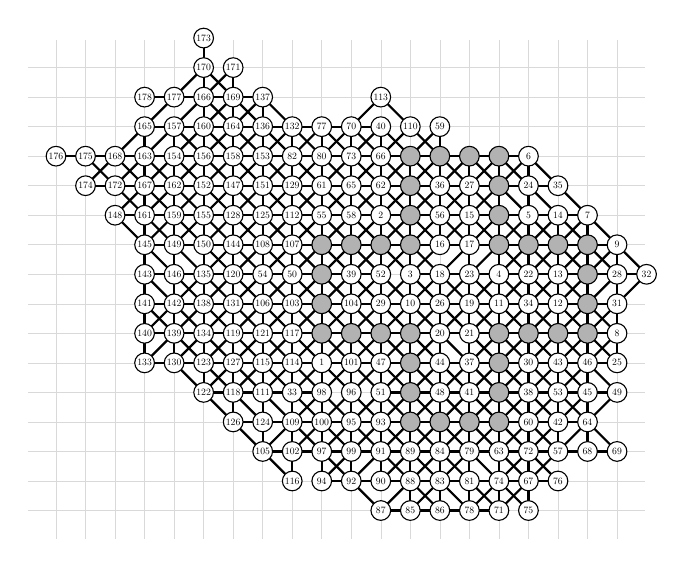
\begin{tikzpicture}[scale=0.75]
\draw[step=2*\unitsize,gray!30,very thin,shift={(-\unitsize, -\unitsize)}] (-27.900000*\unitsize,-15.900000*\unitsize) grid (13.900000*\unitsize,17.900000*\unitsize);
\tikzstyle{every node}=[draw,
			circle,
			fill=white,
			minimum size  = 1*\unitsize,
			node distance = 2*\unitsize,
			inner sep=0pt
			] 


\draw[thick] (-9*\unitsize,-1*\unitsize) -- (-9*\unitsize,1*\unitsize);
    

\draw[thick] (-9*\unitsize,1*\unitsize) -- (-9*\unitsize,3*\unitsize);
    

\draw[thick] (-9*\unitsize,-1*\unitsize) -- (-9*\unitsize,-3*\unitsize);
    

\draw[thick] (-9*\unitsize,-3*\unitsize) -- (-9*\unitsize,-5*\unitsize);
    

\draw[thick] (-5*\unitsize,5*\unitsize) -- (-3*\unitsize,7*\unitsize);
    

\draw[thick] (-3*\unitsize,7*\unitsize) -- (-1*\unitsize,9*\unitsize);
    

\draw[thick] (-5*\unitsize,5*\unitsize) -- (-7*\unitsize,3*\unitsize);
    

\draw[thick] (-7*\unitsize,3*\unitsize) -- (-9*\unitsize,1*\unitsize);
    

\draw[thick] (-3*\unitsize,5*\unitsize) -- (-3*\unitsize,7*\unitsize);
    

\draw[thick] (-3*\unitsize,7*\unitsize) -- (-3*\unitsize,9*\unitsize);
    

\draw[thick] (-3*\unitsize,5*\unitsize) -- (-3*\unitsize,3*\unitsize);
    

\draw[thick] (-3*\unitsize,3*\unitsize) -- (-3*\unitsize,1*\unitsize);
    

\draw[thick] (3*\unitsize,5*\unitsize) -- (3*\unitsize,7*\unitsize);
    

\draw[thick] (3*\unitsize,7*\unitsize) -- (3*\unitsize,9*\unitsize);
    

\draw[thick] (3*\unitsize,5*\unitsize) -- (3*\unitsize,3*\unitsize);
    

\draw[thick] (3*\unitsize,3*\unitsize) -- (3*\unitsize,1*\unitsize);
    

\draw[thick] (5*\unitsize,5*\unitsize) -- (7*\unitsize,3*\unitsize);
    

\draw[thick] (7*\unitsize,3*\unitsize) -- (9*\unitsize,1*\unitsize);
    

\draw[thick] (5*\unitsize,5*\unitsize) -- (3*\unitsize,7*\unitsize);
    

\draw[thick] (3*\unitsize,7*\unitsize) -- (1*\unitsize,9*\unitsize);
    

\draw[thick] (1*\unitsize,9*\unitsize) -- (3*\unitsize,9*\unitsize);
    

\draw[thick] (3*\unitsize,9*\unitsize) -- (5*\unitsize,9*\unitsize);
    

\draw[thick] (1*\unitsize,9*\unitsize) -- (-1*\unitsize,9*\unitsize);
    

\draw[thick] (-1*\unitsize,9*\unitsize) -- (-3*\unitsize,9*\unitsize);
    

\draw[thick] (9*\unitsize,1*\unitsize) -- (9*\unitsize,3*\unitsize);
    

\draw[thick] (9*\unitsize,3*\unitsize) -- (9*\unitsize,5*\unitsize);
    

\draw[thick] (9*\unitsize,1*\unitsize) -- (9*\unitsize,-1*\unitsize);
    

\draw[thick] (9*\unitsize,-1*\unitsize) -- (9*\unitsize,-3*\unitsize);
    

\draw[thick] (7*\unitsize,-3*\unitsize) -- (9*\unitsize,-3*\unitsize);
    

\draw[thick] (9*\unitsize,-3*\unitsize) -- (11*\unitsize,-3*\unitsize);
    

\draw[thick] (7*\unitsize,-3*\unitsize) -- (5*\unitsize,-3*\unitsize);
    

\draw[thick] (5*\unitsize,-3*\unitsize) -- (3*\unitsize,-3*\unitsize);
    

\draw[thick] (7*\unitsize,3*\unitsize) -- (9*\unitsize,3*\unitsize);
    

\draw[thick] (9*\unitsize,3*\unitsize) -- (11*\unitsize,3*\unitsize);
    

\draw[thick] (7*\unitsize,3*\unitsize) -- (5*\unitsize,3*\unitsize);
    

\draw[thick] (5*\unitsize,3*\unitsize) -- (3*\unitsize,3*\unitsize);
    

\draw[thick] (-3*\unitsize,-3*\unitsize) -- (-3*\unitsize,-1*\unitsize);
    

\draw[thick] (-3*\unitsize,-1*\unitsize) -- (-3*\unitsize,1*\unitsize);
    

\draw[thick] (-3*\unitsize,-3*\unitsize) -- (-3*\unitsize,-5*\unitsize);
    

\draw[thick] (-3*\unitsize,-5*\unitsize) -- (-3*\unitsize,-7*\unitsize);
    

\draw[thick] (3*\unitsize,-3*\unitsize) -- (3*\unitsize,-1*\unitsize);
    

\draw[thick] (3*\unitsize,-1*\unitsize) -- (3*\unitsize,1*\unitsize);
    

\draw[thick] (3*\unitsize,-3*\unitsize) -- (3*\unitsize,-5*\unitsize);
    

\draw[thick] (3*\unitsize,-5*\unitsize) -- (3*\unitsize,-7*\unitsize);
    

\draw[thick] (7*\unitsize,-1*\unitsize) -- (9*\unitsize,1*\unitsize);
    

\draw[thick] (9*\unitsize,1*\unitsize) -- (11*\unitsize,3*\unitsize);
    

\draw[thick] (7*\unitsize,-1*\unitsize) -- (5*\unitsize,-3*\unitsize);
    

\draw[thick] (5*\unitsize,-3*\unitsize) -- (3*\unitsize,-5*\unitsize);
    

\draw[thick] (7*\unitsize,1*\unitsize) -- (9*\unitsize,-1*\unitsize);
    

\draw[thick] (9*\unitsize,-1*\unitsize) -- (11*\unitsize,-3*\unitsize);
    

\draw[thick] (7*\unitsize,1*\unitsize) -- (5*\unitsize,3*\unitsize);
    

\draw[thick] (5*\unitsize,3*\unitsize) -- (3*\unitsize,5*\unitsize);
    

\draw[thick] (7*\unitsize,1*\unitsize) -- (7*\unitsize,3*\unitsize);
    

\draw[thick] (7*\unitsize,3*\unitsize) -- (7*\unitsize,5*\unitsize);
    

\draw[thick] (7*\unitsize,1*\unitsize) -- (7*\unitsize,-1*\unitsize);
    

\draw[thick] (7*\unitsize,-1*\unitsize) -- (7*\unitsize,-3*\unitsize);
    

\draw[thick] (5*\unitsize,5*\unitsize) -- (7*\unitsize,5*\unitsize);
    

\draw[thick] (7*\unitsize,5*\unitsize) -- (9*\unitsize,5*\unitsize);
    

\draw[thick] (5*\unitsize,5*\unitsize) -- (3*\unitsize,5*\unitsize);
    

\draw[thick] (3*\unitsize,5*\unitsize) -- (1*\unitsize,5*\unitsize);
    

\draw[thick] (1*\unitsize,5*\unitsize) -- (3*\unitsize,7*\unitsize);
    

\draw[thick] (3*\unitsize,7*\unitsize) -- (5*\unitsize,9*\unitsize);
    

\draw[thick] (1*\unitsize,5*\unitsize) -- (-1*\unitsize,3*\unitsize);
    

\draw[thick] (-1*\unitsize,3*\unitsize) -- (-3*\unitsize,1*\unitsize);
    

\draw[thick] (-1*\unitsize,3*\unitsize) -- (1*\unitsize,3*\unitsize);
    

\draw[thick] (1*\unitsize,3*\unitsize) -- (3*\unitsize,3*\unitsize);
    

\draw[thick] (-1*\unitsize,3*\unitsize) -- (-3*\unitsize,3*\unitsize);
    

\draw[thick] (-3*\unitsize,3*\unitsize) -- (-5*\unitsize,3*\unitsize);
    

\draw[thick] (-1*\unitsize,1*\unitsize) -- (1*\unitsize,3*\unitsize);
    

\draw[thick] (1*\unitsize,3*\unitsize) -- (3*\unitsize,5*\unitsize);
    

\draw[thick] (-1*\unitsize,1*\unitsize) -- (-3*\unitsize,-1*\unitsize);
    

\draw[thick] (-3*\unitsize,-1*\unitsize) -- (-5*\unitsize,-3*\unitsize);
    

\draw[thick] (-1*\unitsize,1*\unitsize) -- (1*\unitsize,-1*\unitsize);
    

\draw[thick] (1*\unitsize,-1*\unitsize) -- (3*\unitsize,-3*\unitsize);
    

\draw[thick] (-1*\unitsize,1*\unitsize) -- (-3*\unitsize,3*\unitsize);
    

\draw[thick] (-3*\unitsize,3*\unitsize) -- (-5*\unitsize,5*\unitsize);
    

\draw[thick] (3*\unitsize,1*\unitsize) -- (5*\unitsize,3*\unitsize);
    

\draw[thick] (5*\unitsize,3*\unitsize) -- (7*\unitsize,5*\unitsize);
    

\draw[thick] (3*\unitsize,1*\unitsize) -- (1*\unitsize,-1*\unitsize);
    

\draw[thick] (1*\unitsize,-1*\unitsize) -- (-1*\unitsize,-3*\unitsize);
    

\draw[thick] (-1*\unitsize,-3*\unitsize) -- (1*\unitsize,-3*\unitsize);
    

\draw[thick] (1*\unitsize,-3*\unitsize) -- (3*\unitsize,-3*\unitsize);
    

\draw[thick] (-1*\unitsize,-3*\unitsize) -- (-3*\unitsize,-3*\unitsize);
    

\draw[thick] (-3*\unitsize,-3*\unitsize) -- (-5*\unitsize,-3*\unitsize);
    

\draw[thick] (5*\unitsize,1*\unitsize) -- (7*\unitsize,3*\unitsize);
    

\draw[thick] (7*\unitsize,3*\unitsize) -- (9*\unitsize,5*\unitsize);
    

\draw[thick] (5*\unitsize,1*\unitsize) -- (3*\unitsize,-1*\unitsize);
    

\draw[thick] (3*\unitsize,-1*\unitsize) -- (1*\unitsize,-3*\unitsize);
    

\draw[thick] (1*\unitsize,1*\unitsize) -- (3*\unitsize,1*\unitsize);
    

\draw[thick] (3*\unitsize,1*\unitsize) -- (5*\unitsize,1*\unitsize);
    

\draw[thick] (1*\unitsize,1*\unitsize) -- (-1*\unitsize,1*\unitsize);
    

\draw[thick] (-1*\unitsize,1*\unitsize) -- (-3*\unitsize,1*\unitsize);
    

\draw[thick] (5*\unitsize,5*\unitsize) -- (5*\unitsize,7*\unitsize);
    

\draw[thick] (5*\unitsize,7*\unitsize) -- (5*\unitsize,9*\unitsize);
    

\draw[thick] (5*\unitsize,5*\unitsize) -- (5*\unitsize,3*\unitsize);
    

\draw[thick] (5*\unitsize,3*\unitsize) -- (5*\unitsize,1*\unitsize);
    

\draw[thick] (7*\unitsize,-1*\unitsize) -- (9*\unitsize,-3*\unitsize);
    

\draw[thick] (9*\unitsize,-3*\unitsize) -- (11*\unitsize,-5*\unitsize);
    

\draw[thick] (7*\unitsize,-1*\unitsize) -- (5*\unitsize,1*\unitsize);
    

\draw[thick] (5*\unitsize,1*\unitsize) -- (3*\unitsize,3*\unitsize);
    

\draw[thick] (1*\unitsize,1*\unitsize) -- (3*\unitsize,3*\unitsize);
    

\draw[thick] (3*\unitsize,3*\unitsize) -- (5*\unitsize,5*\unitsize);
    

\draw[thick] (1*\unitsize,1*\unitsize) -- (-1*\unitsize,-1*\unitsize);
    

\draw[thick] (-1*\unitsize,-1*\unitsize) -- (-3*\unitsize,-3*\unitsize);
    

\draw[thick] (1*\unitsize,5*\unitsize) -- (1*\unitsize,7*\unitsize);
    

\draw[thick] (1*\unitsize,7*\unitsize) -- (1*\unitsize,9*\unitsize);
    

\draw[thick] (1*\unitsize,5*\unitsize) -- (1*\unitsize,3*\unitsize);
    

\draw[thick] (1*\unitsize,3*\unitsize) -- (1*\unitsize,1*\unitsize);
    

\draw[thick] (7*\unitsize,5*\unitsize) -- (9*\unitsize,3*\unitsize);
    

\draw[thick] (9*\unitsize,3*\unitsize) -- (11*\unitsize,1*\unitsize);
    

\draw[thick] (7*\unitsize,5*\unitsize) -- (5*\unitsize,7*\unitsize);
    

\draw[thick] (5*\unitsize,7*\unitsize) -- (3*\unitsize,9*\unitsize);
    

\draw[thick] (-1*\unitsize,-1*\unitsize) -- (1*\unitsize,-1*\unitsize);
    

\draw[thick] (1*\unitsize,-1*\unitsize) -- (3*\unitsize,-1*\unitsize);
    

\draw[thick] (-1*\unitsize,-1*\unitsize) -- (-3*\unitsize,-1*\unitsize);
    

\draw[thick] (-3*\unitsize,-1*\unitsize) -- (-5*\unitsize,-1*\unitsize);
    

\draw[thick] (7*\unitsize,-3*\unitsize) -- (9*\unitsize,-1*\unitsize);
    

\draw[thick] (9*\unitsize,-1*\unitsize) -- (11*\unitsize,1*\unitsize);
    

\draw[thick] (7*\unitsize,-3*\unitsize) -- (5*\unitsize,-5*\unitsize);
    

\draw[thick] (5*\unitsize,-5*\unitsize) -- (3*\unitsize,-7*\unitsize);
    

\draw[thick] (11*\unitsize,-1*\unitsize) -- (11*\unitsize,1*\unitsize);
    

\draw[thick] (11*\unitsize,1*\unitsize) -- (11*\unitsize,3*\unitsize);
    

\draw[thick] (11*\unitsize,-1*\unitsize) -- (11*\unitsize,-3*\unitsize);
    

\draw[thick] (11*\unitsize,-3*\unitsize) -- (11*\unitsize,-5*\unitsize);
    

\draw[thick] (9*\unitsize,1*\unitsize) -- (11*\unitsize,1*\unitsize);
    

\draw[thick] (11*\unitsize,1*\unitsize) -- (13*\unitsize,1*\unitsize);
    

\draw[thick] (9*\unitsize,1*\unitsize) -- (7*\unitsize,1*\unitsize);
    

\draw[thick] (7*\unitsize,1*\unitsize) -- (5*\unitsize,1*\unitsize);
    

\draw[thick] (-7*\unitsize,-3*\unitsize) -- (-5*\unitsize,-1*\unitsize);
    

\draw[thick] (-5*\unitsize,-1*\unitsize) -- (-3*\unitsize,1*\unitsize);
    

\draw[thick] (-7*\unitsize,-3*\unitsize) -- (-9*\unitsize,-5*\unitsize);
    

\draw[thick] (-9*\unitsize,-5*\unitsize) -- (-11*\unitsize,-7*\unitsize);
    

\draw[thick] (7*\unitsize,-1*\unitsize) -- (9*\unitsize,-1*\unitsize);
    

\draw[thick] (9*\unitsize,-1*\unitsize) -- (11*\unitsize,-1*\unitsize);
    

\draw[thick] (7*\unitsize,-1*\unitsize) -- (5*\unitsize,-1*\unitsize);
    

\draw[thick] (5*\unitsize,-1*\unitsize) -- (3*\unitsize,-1*\unitsize);
    

\draw[thick] (9*\unitsize,5*\unitsize) -- (11*\unitsize,3*\unitsize);
    

\draw[thick] (11*\unitsize,3*\unitsize) -- (13*\unitsize,1*\unitsize);
    

\draw[thick] (9*\unitsize,5*\unitsize) -- (7*\unitsize,7*\unitsize);
    

\draw[thick] (7*\unitsize,7*\unitsize) -- (5*\unitsize,9*\unitsize);
    

\draw[thick] (3*\unitsize,7*\unitsize) -- (5*\unitsize,7*\unitsize);
    

\draw[thick] (5*\unitsize,7*\unitsize) -- (7*\unitsize,7*\unitsize);
    

\draw[thick] (3*\unitsize,7*\unitsize) -- (1*\unitsize,7*\unitsize);
    

\draw[thick] (1*\unitsize,7*\unitsize) -- (-1*\unitsize,7*\unitsize);
    

\draw[thick] (5*\unitsize,-1*\unitsize) -- (7*\unitsize,1*\unitsize);
    

\draw[thick] (7*\unitsize,1*\unitsize) -- (9*\unitsize,3*\unitsize);
    

\draw[thick] (5*\unitsize,-1*\unitsize) -- (3*\unitsize,-3*\unitsize);
    

\draw[thick] (3*\unitsize,-3*\unitsize) -- (1*\unitsize,-5*\unitsize);
    

\draw[thick] (5*\unitsize,-3*\unitsize) -- (5*\unitsize,-1*\unitsize);
    

\draw[thick] (5*\unitsize,-1*\unitsize) -- (5*\unitsize,1*\unitsize);
    

\draw[thick] (5*\unitsize,-3*\unitsize) -- (5*\unitsize,-5*\unitsize);
    

\draw[thick] (5*\unitsize,-5*\unitsize) -- (5*\unitsize,-7*\unitsize);
    

\draw[thick] (-3*\unitsize,5*\unitsize) -- (-1*\unitsize,7*\unitsize);
    

\draw[thick] (-1*\unitsize,7*\unitsize) -- (1*\unitsize,9*\unitsize);
    

\draw[thick] (-3*\unitsize,5*\unitsize) -- (-5*\unitsize,3*\unitsize);
    

\draw[thick] (-5*\unitsize,3*\unitsize) -- (-7*\unitsize,1*\unitsize);
    

\draw[thick] (-1*\unitsize,7*\unitsize) -- (1*\unitsize,5*\unitsize);
    

\draw[thick] (1*\unitsize,5*\unitsize) -- (3*\unitsize,3*\unitsize);
    

\draw[thick] (-1*\unitsize,7*\unitsize) -- (-3*\unitsize,9*\unitsize);
    

\draw[thick] (-3*\unitsize,9*\unitsize) -- (-5*\unitsize,11*\unitsize);
    

\draw[thick] (1*\unitsize,-3*\unitsize) -- (1*\unitsize,-1*\unitsize);
    

\draw[thick] (1*\unitsize,-1*\unitsize) -- (1*\unitsize,1*\unitsize);
    

\draw[thick] (1*\unitsize,-3*\unitsize) -- (1*\unitsize,-5*\unitsize);
    

\draw[thick] (1*\unitsize,-5*\unitsize) -- (1*\unitsize,-7*\unitsize);
    

\draw[thick] (3*\unitsize,-5*\unitsize) -- (5*\unitsize,-7*\unitsize);
    

\draw[thick] (5*\unitsize,-7*\unitsize) -- (7*\unitsize,-9*\unitsize);
    

\draw[thick] (3*\unitsize,-5*\unitsize) -- (1*\unitsize,-3*\unitsize);
    

\draw[thick] (1*\unitsize,-3*\unitsize) -- (-1*\unitsize,-1*\unitsize);
    

\draw[thick] (9*\unitsize,-3*\unitsize) -- (11*\unitsize,-1*\unitsize);
    

\draw[thick] (11*\unitsize,-1*\unitsize) -- (13*\unitsize,1*\unitsize);
    

\draw[thick] (9*\unitsize,-3*\unitsize) -- (7*\unitsize,-5*\unitsize);
    

\draw[thick] (7*\unitsize,-5*\unitsize) -- (5*\unitsize,-7*\unitsize);
    

\draw[thick] (-5*\unitsize,-1*\unitsize) -- (-3*\unitsize,-3*\unitsize);
    

\draw[thick] (-3*\unitsize,-3*\unitsize) -- (-1*\unitsize,-5*\unitsize);
    

\draw[thick] (-5*\unitsize,-1*\unitsize) -- (-7*\unitsize,1*\unitsize);
    

\draw[thick] (-7*\unitsize,1*\unitsize) -- (-9*\unitsize,3*\unitsize);
    

\draw[thick] (5*\unitsize,-3*\unitsize) -- (7*\unitsize,-5*\unitsize);
    

\draw[thick] (7*\unitsize,-5*\unitsize) -- (9*\unitsize,-7*\unitsize);
    

\draw[thick] (5*\unitsize,-3*\unitsize) -- (3*\unitsize,-1*\unitsize);
    

\draw[thick] (3*\unitsize,-1*\unitsize) -- (1*\unitsize,1*\unitsize);
    

\draw[thick] (7*\unitsize,-5*\unitsize) -- (9*\unitsize,-5*\unitsize);
    

\draw[thick] (9*\unitsize,-5*\unitsize) -- (11*\unitsize,-5*\unitsize);
    

\draw[thick] (7*\unitsize,-5*\unitsize) -- (5*\unitsize,-5*\unitsize);
    

\draw[thick] (5*\unitsize,-5*\unitsize) -- (3*\unitsize,-5*\unitsize);
    

\draw[thick] (-1*\unitsize,-5*\unitsize) -- (1*\unitsize,-5*\unitsize);
    

\draw[thick] (1*\unitsize,-5*\unitsize) -- (3*\unitsize,-5*\unitsize);
    

\draw[thick] (-1*\unitsize,-5*\unitsize) -- (-3*\unitsize,-5*\unitsize);
    

\draw[thick] (-3*\unitsize,-5*\unitsize) -- (-5*\unitsize,-5*\unitsize);
    

\draw[thick] (-1*\unitsize,-3*\unitsize) -- (-1*\unitsize,-1*\unitsize);
    

\draw[thick] (-1*\unitsize,-1*\unitsize) -- (-1*\unitsize,1*\unitsize);
    

\draw[thick] (-1*\unitsize,-3*\unitsize) -- (-1*\unitsize,-5*\unitsize);
    

\draw[thick] (-1*\unitsize,-5*\unitsize) -- (-1*\unitsize,-7*\unitsize);
    

\draw[thick] (7*\unitsize,-3*\unitsize) -- (9*\unitsize,-5*\unitsize);
    

\draw[thick] (9*\unitsize,-5*\unitsize) -- (11*\unitsize,-7*\unitsize);
    

\draw[thick] (7*\unitsize,-3*\unitsize) -- (5*\unitsize,-1*\unitsize);
    

\draw[thick] (5*\unitsize,-1*\unitsize) -- (3*\unitsize,1*\unitsize);
    

\draw[thick] (-7*\unitsize,-3*\unitsize) -- (-5*\unitsize,-5*\unitsize);
    

\draw[thick] (-5*\unitsize,-5*\unitsize) -- (-3*\unitsize,-7*\unitsize);
    

\draw[thick] (-7*\unitsize,-3*\unitsize) -- (-9*\unitsize,-1*\unitsize);
    

\draw[thick] (-9*\unitsize,-1*\unitsize) -- (-11*\unitsize,1*\unitsize);
    

\draw[thick] (-1*\unitsize,-7*\unitsize) -- (1*\unitsize,-7*\unitsize);
    

\draw[thick] (1*\unitsize,-7*\unitsize) -- (3*\unitsize,-7*\unitsize);
    

\draw[thick] (-1*\unitsize,-7*\unitsize) -- (-3*\unitsize,-7*\unitsize);
    

\draw[thick] (-3*\unitsize,-7*\unitsize) -- (-5*\unitsize,-7*\unitsize);
    

\draw[thick] (-5*\unitsize,-1*\unitsize) -- (-5*\unitsize,1*\unitsize);
    

\draw[thick] (-5*\unitsize,1*\unitsize) -- (-5*\unitsize,3*\unitsize);
    

\draw[thick] (-5*\unitsize,-1*\unitsize) -- (-5*\unitsize,-3*\unitsize);
    

\draw[thick] (-5*\unitsize,-3*\unitsize) -- (-5*\unitsize,-5*\unitsize);
    

\draw[thick] (7*\unitsize,-7*\unitsize) -- (9*\unitsize,-7*\unitsize);
    

\draw[thick] (9*\unitsize,-7*\unitsize) -- (11*\unitsize,-7*\unitsize);
    

\draw[thick] (7*\unitsize,-7*\unitsize) -- (5*\unitsize,-7*\unitsize);
    

\draw[thick] (5*\unitsize,-7*\unitsize) -- (3*\unitsize,-7*\unitsize);
    

\draw[thick] (-9*\unitsize,1*\unitsize) -- (-7*\unitsize,1*\unitsize);
    

\draw[thick] (-7*\unitsize,1*\unitsize) -- (-5*\unitsize,1*\unitsize);
    

\draw[thick] (-9*\unitsize,1*\unitsize) -- (-11*\unitsize,1*\unitsize);
    

\draw[thick] (-11*\unitsize,1*\unitsize) -- (-13*\unitsize,1*\unitsize);
    

\draw[thick] (-5*\unitsize,1*\unitsize) -- (-3*\unitsize,-1*\unitsize);
    

\draw[thick] (-3*\unitsize,-1*\unitsize) -- (-1*\unitsize,-3*\unitsize);
    

\draw[thick] (-5*\unitsize,1*\unitsize) -- (-7*\unitsize,3*\unitsize);
    

\draw[thick] (-7*\unitsize,3*\unitsize) -- (-9*\unitsize,5*\unitsize);
    

\draw[thick] (-1*\unitsize,5*\unitsize) -- (1*\unitsize,7*\unitsize);
    

\draw[thick] (1*\unitsize,7*\unitsize) -- (3*\unitsize,9*\unitsize);
    

\draw[thick] (-1*\unitsize,5*\unitsize) -- (-3*\unitsize,3*\unitsize);
    

\draw[thick] (-3*\unitsize,3*\unitsize) -- (-5*\unitsize,1*\unitsize);
    

\draw[thick] (7*\unitsize,-7*\unitsize) -- (7*\unitsize,-5*\unitsize);
    

\draw[thick] (7*\unitsize,-5*\unitsize) -- (7*\unitsize,-3*\unitsize);
    

\draw[thick] (7*\unitsize,-7*\unitsize) -- (7*\unitsize,-9*\unitsize);
    

\draw[thick] (7*\unitsize,-9*\unitsize) -- (7*\unitsize,-11*\unitsize);
    

\draw[thick] (-3*\unitsize,5*\unitsize) -- (-1*\unitsize,5*\unitsize);
    

\draw[thick] (-1*\unitsize,5*\unitsize) -- (1*\unitsize,5*\unitsize);
    

\draw[thick] (-3*\unitsize,5*\unitsize) -- (-5*\unitsize,5*\unitsize);
    

\draw[thick] (-5*\unitsize,5*\unitsize) -- (-7*\unitsize,5*\unitsize);
    

\draw[thick] (-1*\unitsize,7*\unitsize) -- (-1*\unitsize,9*\unitsize);
    

\draw[thick] (-1*\unitsize,9*\unitsize) -- (-1*\unitsize,11*\unitsize);
    

\draw[thick] (-1*\unitsize,7*\unitsize) -- (-1*\unitsize,5*\unitsize);
    

\draw[thick] (-1*\unitsize,5*\unitsize) -- (-1*\unitsize,3*\unitsize);
    

\draw[thick] (3*\unitsize,-7*\unitsize) -- (5*\unitsize,-9*\unitsize);
    

\draw[thick] (5*\unitsize,-9*\unitsize) -- (7*\unitsize,-11*\unitsize);
    

\draw[thick] (3*\unitsize,-7*\unitsize) -- (1*\unitsize,-5*\unitsize);
    

\draw[thick] (1*\unitsize,-5*\unitsize) -- (-1*\unitsize,-3*\unitsize);
    

\draw[thick] (-5*\unitsize,3*\unitsize) -- (-3*\unitsize,1*\unitsize);
    

\draw[thick] (-3*\unitsize,1*\unitsize) -- (-1*\unitsize,-1*\unitsize);
    

\draw[thick] (-5*\unitsize,3*\unitsize) -- (-7*\unitsize,5*\unitsize);
    

\draw[thick] (-7*\unitsize,5*\unitsize) -- (-9*\unitsize,7*\unitsize);
    

\draw[thick] (-5*\unitsize,7*\unitsize) -- (-3*\unitsize,9*\unitsize);
    

\draw[thick] (-3*\unitsize,9*\unitsize) -- (-1*\unitsize,11*\unitsize);
    

\draw[thick] (-5*\unitsize,7*\unitsize) -- (-7*\unitsize,5*\unitsize);
    

\draw[thick] (-7*\unitsize,5*\unitsize) -- (-9*\unitsize,3*\unitsize);
    

\draw[thick] (7*\unitsize,-7*\unitsize) -- (9*\unitsize,-5*\unitsize);
    

\draw[thick] (9*\unitsize,-5*\unitsize) -- (11*\unitsize,-3*\unitsize);
    

\draw[thick] (7*\unitsize,-7*\unitsize) -- (5*\unitsize,-9*\unitsize);
    

\draw[thick] (5*\unitsize,-9*\unitsize) -- (3*\unitsize,-11*\unitsize);
    

\draw[thick] (5*\unitsize,-9*\unitsize) -- (7*\unitsize,-9*\unitsize);
    

\draw[thick] (7*\unitsize,-9*\unitsize) -- (9*\unitsize,-9*\unitsize);
    

\draw[thick] (5*\unitsize,-9*\unitsize) -- (3*\unitsize,-9*\unitsize);
    

\draw[thick] (3*\unitsize,-9*\unitsize) -- (1*\unitsize,-9*\unitsize);
    

\draw[thick] (-5*\unitsize,7*\unitsize) -- (-3*\unitsize,7*\unitsize);
    

\draw[thick] (-3*\unitsize,7*\unitsize) -- (-1*\unitsize,7*\unitsize);
    

\draw[thick] (-5*\unitsize,7*\unitsize) -- (-7*\unitsize,7*\unitsize);
    

\draw[thick] (-7*\unitsize,7*\unitsize) -- (-9*\unitsize,7*\unitsize);
    

\draw[thick] (-5*\unitsize,7*\unitsize) -- (-5*\unitsize,9*\unitsize);
    

\draw[thick] (-5*\unitsize,9*\unitsize) -- (-5*\unitsize,11*\unitsize);
    

\draw[thick] (-5*\unitsize,7*\unitsize) -- (-5*\unitsize,5*\unitsize);
    

\draw[thick] (-5*\unitsize,5*\unitsize) -- (-5*\unitsize,3*\unitsize);
    

\draw[thick] (1*\unitsize,-9*\unitsize) -- (3*\unitsize,-11*\unitsize);
    

\draw[thick] (3*\unitsize,-11*\unitsize) -- (5*\unitsize,-13*\unitsize);
    

\draw[thick] (1*\unitsize,-9*\unitsize) -- (-1*\unitsize,-7*\unitsize);
    

\draw[thick] (-1*\unitsize,-7*\unitsize) -- (-3*\unitsize,-5*\unitsize);
    

\draw[thick] (9*\unitsize,-7*\unitsize) -- (9*\unitsize,-5*\unitsize);
    

\draw[thick] (9*\unitsize,-5*\unitsize) -- (9*\unitsize,-3*\unitsize);
    

\draw[thick] (9*\unitsize,-7*\unitsize) -- (9*\unitsize,-9*\unitsize);
    

\draw[thick] (9*\unitsize,-9*\unitsize) -- (9*\unitsize,-11*\unitsize);
    

\draw[thick] (7*\unitsize,-7*\unitsize) -- (9*\unitsize,-9*\unitsize);
    

\draw[thick] (9*\unitsize,-9*\unitsize) -- (11*\unitsize,-11*\unitsize);
    

\draw[thick] (7*\unitsize,-7*\unitsize) -- (5*\unitsize,-5*\unitsize);
    

\draw[thick] (5*\unitsize,-5*\unitsize) -- (3*\unitsize,-3*\unitsize);
    

\draw[thick] (-3*\unitsize,7*\unitsize) -- (-1*\unitsize,5*\unitsize);
    

\draw[thick] (-1*\unitsize,5*\unitsize) -- (1*\unitsize,3*\unitsize);
    

\draw[thick] (-3*\unitsize,7*\unitsize) -- (-5*\unitsize,9*\unitsize);
    

\draw[thick] (-5*\unitsize,9*\unitsize) -- (-7*\unitsize,11*\unitsize);
    

\draw[thick] (7*\unitsize,-11*\unitsize) -- (9*\unitsize,-9*\unitsize);
    

\draw[thick] (9*\unitsize,-9*\unitsize) -- (11*\unitsize,-7*\unitsize);
    

\draw[thick] (7*\unitsize,-11*\unitsize) -- (5*\unitsize,-13*\unitsize);
    

\draw[thick] (5*\unitsize,-13*\unitsize) -- (3*\unitsize,-15*\unitsize);
    

\draw[thick] (7*\unitsize,-11*\unitsize) -- (9*\unitsize,-11*\unitsize);
    

\draw[thick] (9*\unitsize,-11*\unitsize) -- (11*\unitsize,-11*\unitsize);
    

\draw[thick] (7*\unitsize,-11*\unitsize) -- (5*\unitsize,-11*\unitsize);
    

\draw[thick] (5*\unitsize,-11*\unitsize) -- (3*\unitsize,-11*\unitsize);
    

\draw[thick] (-7*\unitsize,7*\unitsize) -- (-7*\unitsize,9*\unitsize);
    

\draw[thick] (-7*\unitsize,9*\unitsize) -- (-7*\unitsize,11*\unitsize);
    

\draw[thick] (-7*\unitsize,7*\unitsize) -- (-7*\unitsize,5*\unitsize);
    

\draw[thick] (-7*\unitsize,5*\unitsize) -- (-7*\unitsize,3*\unitsize);
    

\draw[thick] (3*\unitsize,-11*\unitsize) -- (3*\unitsize,-9*\unitsize);
    

\draw[thick] (3*\unitsize,-9*\unitsize) -- (3*\unitsize,-7*\unitsize);
    

\draw[thick] (3*\unitsize,-11*\unitsize) -- (3*\unitsize,-13*\unitsize);
    

\draw[thick] (3*\unitsize,-13*\unitsize) -- (3*\unitsize,-15*\unitsize);
    

\draw[thick] (5*\unitsize,-11*\unitsize) -- (5*\unitsize,-9*\unitsize);
    

\draw[thick] (5*\unitsize,-9*\unitsize) -- (5*\unitsize,-7*\unitsize);
    

\draw[thick] (5*\unitsize,-11*\unitsize) -- (5*\unitsize,-13*\unitsize);
    

\draw[thick] (5*\unitsize,-13*\unitsize) -- (5*\unitsize,-15*\unitsize);
    

\draw[thick] (3*\unitsize,-9*\unitsize) -- (5*\unitsize,-11*\unitsize);
    

\draw[thick] (5*\unitsize,-11*\unitsize) -- (7*\unitsize,-13*\unitsize);
    

\draw[thick] (3*\unitsize,-9*\unitsize) -- (1*\unitsize,-7*\unitsize);
    

\draw[thick] (1*\unitsize,-7*\unitsize) -- (-1*\unitsize,-5*\unitsize);
    

\draw[thick] (-5*\unitsize,7*\unitsize) -- (-3*\unitsize,5*\unitsize);
    

\draw[thick] (-3*\unitsize,5*\unitsize) -- (-1*\unitsize,3*\unitsize);
    

\draw[thick] (-5*\unitsize,7*\unitsize) -- (-7*\unitsize,9*\unitsize);
    

\draw[thick] (-7*\unitsize,9*\unitsize) -- (-9*\unitsize,11*\unitsize);
    

\draw[thick] (5*\unitsize,-11*\unitsize) -- (7*\unitsize,-9*\unitsize);
    

\draw[thick] (7*\unitsize,-9*\unitsize) -- (9*\unitsize,-7*\unitsize);
    

\draw[thick] (5*\unitsize,-11*\unitsize) -- (3*\unitsize,-13*\unitsize);
    

\draw[thick] (3*\unitsize,-13*\unitsize) -- (1*\unitsize,-15*\unitsize);
    

\draw[thick] (1*\unitsize,-11*\unitsize) -- (3*\unitsize,-13*\unitsize);
    

\draw[thick] (3*\unitsize,-13*\unitsize) -- (5*\unitsize,-15*\unitsize);
    

\draw[thick] (1*\unitsize,-11*\unitsize) -- (-1*\unitsize,-9*\unitsize);
    

\draw[thick] (-1*\unitsize,-9*\unitsize) -- (-3*\unitsize,-7*\unitsize);
    

\draw[thick] (-9*\unitsize,7*\unitsize) -- (-9*\unitsize,9*\unitsize);
    

\draw[thick] (-9*\unitsize,9*\unitsize) -- (-9*\unitsize,11*\unitsize);
    

\draw[thick] (-9*\unitsize,7*\unitsize) -- (-9*\unitsize,5*\unitsize);
    

\draw[thick] (-9*\unitsize,5*\unitsize) -- (-9*\unitsize,3*\unitsize);
    

\draw[thick] (1*\unitsize,-11*\unitsize) -- (1*\unitsize,-9*\unitsize);
    

\draw[thick] (1*\unitsize,-9*\unitsize) -- (1*\unitsize,-7*\unitsize);
    

\draw[thick] (1*\unitsize,-11*\unitsize) -- (1*\unitsize,-13*\unitsize);
    

\draw[thick] (1*\unitsize,-13*\unitsize) -- (1*\unitsize,-15*\unitsize);
    

\draw[thick] (-7*\unitsize,9*\unitsize) -- (-5*\unitsize,9*\unitsize);
    

\draw[thick] (-5*\unitsize,9*\unitsize) -- (-3*\unitsize,9*\unitsize);
    

\draw[thick] (-7*\unitsize,9*\unitsize) -- (-9*\unitsize,9*\unitsize);
    

\draw[thick] (-9*\unitsize,9*\unitsize) -- (-11*\unitsize,9*\unitsize);
    

\draw[thick] (3*\unitsize,-13*\unitsize) -- (5*\unitsize,-13*\unitsize);
    

\draw[thick] (5*\unitsize,-13*\unitsize) -- (7*\unitsize,-13*\unitsize);
    

\draw[thick] (3*\unitsize,-13*\unitsize) -- (1*\unitsize,-13*\unitsize);
    

\draw[thick] (1*\unitsize,-13*\unitsize) -- (-1*\unitsize,-13*\unitsize);
    

\draw[thick] (-1*\unitsize,-11*\unitsize) -- (1*\unitsize,-13*\unitsize);
    

\draw[thick] (1*\unitsize,-13*\unitsize) -- (3*\unitsize,-15*\unitsize);
    

\draw[thick] (-1*\unitsize,-11*\unitsize) -- (-3*\unitsize,-9*\unitsize);
    

\draw[thick] (-3*\unitsize,-9*\unitsize) -- (-5*\unitsize,-7*\unitsize);
    

\draw[thick] (1*\unitsize,-11*\unitsize) -- (3*\unitsize,-9*\unitsize);
    

\draw[thick] (3*\unitsize,-9*\unitsize) -- (5*\unitsize,-7*\unitsize);
    

\draw[thick] (1*\unitsize,-11*\unitsize) -- (-1*\unitsize,-13*\unitsize);
    

\draw[thick] (-1*\unitsize,-13*\unitsize) -- (-3*\unitsize,-15*\unitsize);
    

\draw[thick] (-1*\unitsize,-11*\unitsize) -- (-1*\unitsize,-9*\unitsize);
    

\draw[thick] (-1*\unitsize,-9*\unitsize) -- (-1*\unitsize,-7*\unitsize);
    

\draw[thick] (-1*\unitsize,-11*\unitsize) -- (-1*\unitsize,-13*\unitsize);
    

\draw[thick] (-1*\unitsize,-13*\unitsize) -- (-1*\unitsize,-15*\unitsize);
    

\draw[thick] (-1*\unitsize,-15*\unitsize) -- (1*\unitsize,-15*\unitsize);
    

\draw[thick] (1*\unitsize,-15*\unitsize) -- (3*\unitsize,-15*\unitsize);
    

\draw[thick] (-1*\unitsize,-15*\unitsize) -- (-3*\unitsize,-15*\unitsize);
    

\draw[thick] (-3*\unitsize,-15*\unitsize) -- (-5*\unitsize,-15*\unitsize);
    

\draw[thick] (-1*\unitsize,-11*\unitsize) -- (1*\unitsize,-9*\unitsize);
    

\draw[thick] (1*\unitsize,-9*\unitsize) -- (3*\unitsize,-7*\unitsize);
    

\draw[thick] (-1*\unitsize,-11*\unitsize) -- (-3*\unitsize,-13*\unitsize);
    

\draw[thick] (-3*\unitsize,-13*\unitsize) -- (-5*\unitsize,-15*\unitsize);
    

\draw[thick] (-3*\unitsize,-11*\unitsize) -- (-3*\unitsize,-9*\unitsize);
    

\draw[thick] (-3*\unitsize,-9*\unitsize) -- (-3*\unitsize,-7*\unitsize);
    

\draw[thick] (-3*\unitsize,-11*\unitsize) -- (-3*\unitsize,-13*\unitsize);
    

\draw[thick] (-3*\unitsize,-13*\unitsize) -- (-3*\unitsize,-15*\unitsize);
    

\draw[thick] (-1*\unitsize,-9*\unitsize) -- (1*\unitsize,-7*\unitsize);
    

\draw[thick] (1*\unitsize,-7*\unitsize) -- (3*\unitsize,-5*\unitsize);
    

\draw[thick] (-1*\unitsize,-9*\unitsize) -- (-3*\unitsize,-11*\unitsize);
    

\draw[thick] (-3*\unitsize,-11*\unitsize) -- (-5*\unitsize,-13*\unitsize);
    

\draw[thick] (-1*\unitsize,-11*\unitsize) -- (1*\unitsize,-11*\unitsize);
    

\draw[thick] (1*\unitsize,-11*\unitsize) -- (3*\unitsize,-11*\unitsize);
    

\draw[thick] (-1*\unitsize,-11*\unitsize) -- (-3*\unitsize,-11*\unitsize);
    

\draw[thick] (-3*\unitsize,-11*\unitsize) -- (-5*\unitsize,-11*\unitsize);
    

\draw[thick] (-3*\unitsize,-9*\unitsize) -- (-1*\unitsize,-7*\unitsize);
    

\draw[thick] (-1*\unitsize,-7*\unitsize) -- (1*\unitsize,-5*\unitsize);
    

\draw[thick] (-3*\unitsize,-9*\unitsize) -- (-5*\unitsize,-11*\unitsize);
    

\draw[thick] (-5*\unitsize,-11*\unitsize) -- (-7*\unitsize,-13*\unitsize);
    

\draw[thick] (-5*\unitsize,-9*\unitsize) -- (-5*\unitsize,-7*\unitsize);
    

\draw[thick] (-5*\unitsize,-7*\unitsize) -- (-5*\unitsize,-5*\unitsize);
    

\draw[thick] (-5*\unitsize,-9*\unitsize) -- (-5*\unitsize,-11*\unitsize);
    

\draw[thick] (-5*\unitsize,-11*\unitsize) -- (-5*\unitsize,-13*\unitsize);
    

\draw[thick] (-5*\unitsize,-13*\unitsize) -- (-3*\unitsize,-13*\unitsize);
    

\draw[thick] (-3*\unitsize,-13*\unitsize) -- (-1*\unitsize,-13*\unitsize);
    

\draw[thick] (-5*\unitsize,-13*\unitsize) -- (-7*\unitsize,-13*\unitsize);
    

\draw[thick] (-7*\unitsize,-13*\unitsize) -- (-9*\unitsize,-13*\unitsize);
    

\draw[thick] (-3*\unitsize,-9*\unitsize) -- (-1*\unitsize,-9*\unitsize);
    

\draw[thick] (-1*\unitsize,-9*\unitsize) -- (1*\unitsize,-9*\unitsize);
    

\draw[thick] (-3*\unitsize,-9*\unitsize) -- (-5*\unitsize,-9*\unitsize);
    

\draw[thick] (-5*\unitsize,-9*\unitsize) -- (-7*\unitsize,-9*\unitsize);
    

\draw[thick] (-3*\unitsize,-11*\unitsize) -- (-1*\unitsize,-13*\unitsize);
    

\draw[thick] (-1*\unitsize,-13*\unitsize) -- (1*\unitsize,-15*\unitsize);
    

\draw[thick] (-3*\unitsize,-11*\unitsize) -- (-5*\unitsize,-9*\unitsize);
    

\draw[thick] (-5*\unitsize,-9*\unitsize) -- (-7*\unitsize,-7*\unitsize);
    

\draw[thick] (-5*\unitsize,-7*\unitsize) -- (-3*\unitsize,-5*\unitsize);
    

\draw[thick] (-3*\unitsize,-5*\unitsize) -- (-1*\unitsize,-3*\unitsize);
    

\draw[thick] (-5*\unitsize,-7*\unitsize) -- (-7*\unitsize,-9*\unitsize);
    

\draw[thick] (-7*\unitsize,-9*\unitsize) -- (-9*\unitsize,-11*\unitsize);
    

\draw[thick] (-5*\unitsize,-11*\unitsize) -- (-3*\unitsize,-13*\unitsize);
    

\draw[thick] (-3*\unitsize,-13*\unitsize) -- (-1*\unitsize,-15*\unitsize);
    

\draw[thick] (-5*\unitsize,-11*\unitsize) -- (-7*\unitsize,-9*\unitsize);
    

\draw[thick] (-7*\unitsize,-9*\unitsize) -- (-9*\unitsize,-7*\unitsize);
    

\draw[thick] (-5*\unitsize,-9*\unitsize) -- (-3*\unitsize,-7*\unitsize);
    

\draw[thick] (-3*\unitsize,-7*\unitsize) -- (-1*\unitsize,-5*\unitsize);
    

\draw[thick] (-5*\unitsize,-9*\unitsize) -- (-7*\unitsize,-11*\unitsize);
    

\draw[thick] (-7*\unitsize,-11*\unitsize) -- (-9*\unitsize,-13*\unitsize);
    

\draw[thick] (-9*\unitsize,-9*\unitsize) -- (-9*\unitsize,-7*\unitsize);
    

\draw[thick] (-9*\unitsize,-7*\unitsize) -- (-9*\unitsize,-5*\unitsize);
    

\draw[thick] (-9*\unitsize,-9*\unitsize) -- (-9*\unitsize,-11*\unitsize);
    

\draw[thick] (-9*\unitsize,-11*\unitsize) -- (-9*\unitsize,-13*\unitsize);
    

\draw[thick] (-7*\unitsize,-9*\unitsize) -- (-7*\unitsize,-7*\unitsize);
    

\draw[thick] (-7*\unitsize,-7*\unitsize) -- (-7*\unitsize,-5*\unitsize);
    

\draw[thick] (-7*\unitsize,-9*\unitsize) -- (-7*\unitsize,-11*\unitsize);
    

\draw[thick] (-7*\unitsize,-11*\unitsize) -- (-7*\unitsize,-13*\unitsize);
    

\draw[thick] (-7*\unitsize,-7*\unitsize) -- (-5*\unitsize,-5*\unitsize);
    

\draw[thick] (-5*\unitsize,-5*\unitsize) -- (-3*\unitsize,-3*\unitsize);
    

\draw[thick] (-7*\unitsize,-7*\unitsize) -- (-9*\unitsize,-9*\unitsize);
    

\draw[thick] (-9*\unitsize,-9*\unitsize) -- (-11*\unitsize,-11*\unitsize);
    

\draw[thick] (-9*\unitsize,-3*\unitsize) -- (-7*\unitsize,-5*\unitsize);
    

\draw[thick] (-7*\unitsize,-5*\unitsize) -- (-5*\unitsize,-7*\unitsize);
    

\draw[thick] (-9*\unitsize,-3*\unitsize) -- (-11*\unitsize,-1*\unitsize);
    

\draw[thick] (-11*\unitsize,-1*\unitsize) -- (-13*\unitsize,1*\unitsize);
    

\draw[thick] (-7*\unitsize,-1*\unitsize) -- (-7*\unitsize,1*\unitsize);
    

\draw[thick] (-7*\unitsize,1*\unitsize) -- (-7*\unitsize,3*\unitsize);
    

\draw[thick] (-7*\unitsize,-1*\unitsize) -- (-7*\unitsize,-3*\unitsize);
    

\draw[thick] (-7*\unitsize,-3*\unitsize) -- (-7*\unitsize,-5*\unitsize);
    

\draw[thick] (-9*\unitsize,-11*\unitsize) -- (-7*\unitsize,-11*\unitsize);
    

\draw[thick] (-7*\unitsize,-11*\unitsize) -- (-5*\unitsize,-11*\unitsize);
    

\draw[thick] (-9*\unitsize,-11*\unitsize) -- (-11*\unitsize,-11*\unitsize);
    

\draw[thick] (-11*\unitsize,-11*\unitsize) -- (-13*\unitsize,-11*\unitsize);
    

\draw[thick] (-9*\unitsize,-1*\unitsize) -- (-7*\unitsize,-1*\unitsize);
    

\draw[thick] (-7*\unitsize,-1*\unitsize) -- (-5*\unitsize,-1*\unitsize);
    

\draw[thick] (-9*\unitsize,-1*\unitsize) -- (-11*\unitsize,-1*\unitsize);
    

\draw[thick] (-11*\unitsize,-1*\unitsize) -- (-13*\unitsize,-1*\unitsize);
    

\draw[thick] (-7*\unitsize,-1*\unitsize) -- (-5*\unitsize,-3*\unitsize);
    

\draw[thick] (-5*\unitsize,-3*\unitsize) -- (-3*\unitsize,-5*\unitsize);
    

\draw[thick] (-7*\unitsize,-1*\unitsize) -- (-9*\unitsize,1*\unitsize);
    

\draw[thick] (-9*\unitsize,1*\unitsize) -- (-11*\unitsize,3*\unitsize);
    

\draw[thick] (-9*\unitsize,3*\unitsize) -- (-7*\unitsize,3*\unitsize);
    

\draw[thick] (-7*\unitsize,3*\unitsize) -- (-5*\unitsize,3*\unitsize);
    

\draw[thick] (-9*\unitsize,3*\unitsize) -- (-11*\unitsize,3*\unitsize);
    

\draw[thick] (-11*\unitsize,3*\unitsize) -- (-13*\unitsize,3*\unitsize);
    

\draw[thick] (-9*\unitsize,-7*\unitsize) -- (-7*\unitsize,-5*\unitsize);
    

\draw[thick] (-7*\unitsize,-5*\unitsize) -- (-5*\unitsize,-3*\unitsize);
    

\draw[thick] (-9*\unitsize,-7*\unitsize) -- (-11*\unitsize,-9*\unitsize);
    

\draw[thick] (-11*\unitsize,-9*\unitsize) -- (-13*\unitsize,-11*\unitsize);
    

\draw[thick] (-7*\unitsize,7*\unitsize) -- (-5*\unitsize,9*\unitsize);
    

\draw[thick] (-5*\unitsize,9*\unitsize) -- (-3*\unitsize,11*\unitsize);
    

\draw[thick] (-7*\unitsize,7*\unitsize) -- (-9*\unitsize,5*\unitsize);
    

\draw[thick] (-9*\unitsize,5*\unitsize) -- (-11*\unitsize,3*\unitsize);
    

\draw[thick] (-9*\unitsize,-11*\unitsize) -- (-7*\unitsize,-13*\unitsize);
    

\draw[thick] (-7*\unitsize,-13*\unitsize) -- (-5*\unitsize,-15*\unitsize);
    

\draw[thick] (-9*\unitsize,-11*\unitsize) -- (-11*\unitsize,-9*\unitsize);
    

\draw[thick] (-11*\unitsize,-9*\unitsize) -- (-13*\unitsize,-7*\unitsize);
    

\draw[thick] (-9*\unitsize,7*\unitsize) -- (-7*\unitsize,9*\unitsize);
    

\draw[thick] (-7*\unitsize,9*\unitsize) -- (-5*\unitsize,11*\unitsize);
    

\draw[thick] (-9*\unitsize,7*\unitsize) -- (-11*\unitsize,5*\unitsize);
    

\draw[thick] (-11*\unitsize,5*\unitsize) -- (-13*\unitsize,3*\unitsize);
    

\draw[thick] (-1*\unitsize,9*\unitsize) -- (1*\unitsize,7*\unitsize);
    

\draw[thick] (1*\unitsize,7*\unitsize) -- (3*\unitsize,5*\unitsize);
    

\draw[thick] (-1*\unitsize,9*\unitsize) -- (-3*\unitsize,11*\unitsize);
    

\draw[thick] (-3*\unitsize,11*\unitsize) -- (-5*\unitsize,13*\unitsize);
    

\draw[thick] (-9*\unitsize,-3*\unitsize) -- (-7*\unitsize,-1*\unitsize);
    

\draw[thick] (-7*\unitsize,-1*\unitsize) -- (-5*\unitsize,1*\unitsize);
    

\draw[thick] (-9*\unitsize,-3*\unitsize) -- (-11*\unitsize,-5*\unitsize);
    

\draw[thick] (-11*\unitsize,-5*\unitsize) -- (-13*\unitsize,-7*\unitsize);
    

\draw[thick] (-9*\unitsize,-5*\unitsize) -- (-7*\unitsize,-5*\unitsize);
    

\draw[thick] (-7*\unitsize,-5*\unitsize) -- (-5*\unitsize,-5*\unitsize);
    

\draw[thick] (-9*\unitsize,-5*\unitsize) -- (-11*\unitsize,-5*\unitsize);
    

\draw[thick] (-11*\unitsize,-5*\unitsize) -- (-13*\unitsize,-5*\unitsize);
    

\draw[thick] (-11*\unitsize,-9*\unitsize) -- (-11*\unitsize,-7*\unitsize);
    

\draw[thick] (-11*\unitsize,-7*\unitsize) -- (-11*\unitsize,-5*\unitsize);
    

\draw[thick] (-11*\unitsize,-9*\unitsize) -- (-11*\unitsize,-11*\unitsize);
    

\draw[thick] (-11*\unitsize,-11*\unitsize) -- (-11*\unitsize,-13*\unitsize);
    

\draw[thick] (-11*\unitsize,-1*\unitsize) -- (-11*\unitsize,1*\unitsize);
    

\draw[thick] (-11*\unitsize,1*\unitsize) -- (-11*\unitsize,3*\unitsize);
    

\draw[thick] (-11*\unitsize,-1*\unitsize) -- (-11*\unitsize,-3*\unitsize);
    

\draw[thick] (-11*\unitsize,-3*\unitsize) -- (-11*\unitsize,-5*\unitsize);
    

\draw[thick] (-11*\unitsize,-3*\unitsize) -- (-9*\unitsize,-1*\unitsize);
    

\draw[thick] (-9*\unitsize,-1*\unitsize) -- (-7*\unitsize,1*\unitsize);
    

\draw[thick] (-11*\unitsize,-3*\unitsize) -- (-13*\unitsize,-5*\unitsize);
    

\draw[thick] (-13*\unitsize,-5*\unitsize) -- (-15*\unitsize,-7*\unitsize);
    

\draw[thick] (-11*\unitsize,-7*\unitsize) -- (-9*\unitsize,-9*\unitsize);
    

\draw[thick] (-9*\unitsize,-9*\unitsize) -- (-7*\unitsize,-11*\unitsize);
    

\draw[thick] (-11*\unitsize,-7*\unitsize) -- (-13*\unitsize,-5*\unitsize);
    

\draw[thick] (-13*\unitsize,-5*\unitsize) -- (-15*\unitsize,-3*\unitsize);
    

\draw[thick] (-11*\unitsize,-3*\unitsize) -- (-9*\unitsize,-5*\unitsize);
    

\draw[thick] (-9*\unitsize,-5*\unitsize) -- (-7*\unitsize,-7*\unitsize);
    

\draw[thick] (-11*\unitsize,-3*\unitsize) -- (-13*\unitsize,-1*\unitsize);
    

\draw[thick] (-13*\unitsize,-1*\unitsize) -- (-15*\unitsize,1*\unitsize);
    

\draw[thick] (-9*\unitsize,-3*\unitsize) -- (-7*\unitsize,-3*\unitsize);
    

\draw[thick] (-7*\unitsize,-3*\unitsize) -- (-5*\unitsize,-3*\unitsize);
    

\draw[thick] (-9*\unitsize,-3*\unitsize) -- (-11*\unitsize,-3*\unitsize);
    

\draw[thick] (-11*\unitsize,-3*\unitsize) -- (-13*\unitsize,-3*\unitsize);
    

\draw[thick] (-13*\unitsize,-7*\unitsize) -- (-11*\unitsize,-7*\unitsize);
    

\draw[thick] (-11*\unitsize,-7*\unitsize) -- (-9*\unitsize,-7*\unitsize);
    

\draw[thick] (-13*\unitsize,-7*\unitsize) -- (-15*\unitsize,-7*\unitsize);
    

\draw[thick] (-15*\unitsize,-7*\unitsize) -- (-17*\unitsize,-7*\unitsize);
    

\draw[thick] (-13*\unitsize,-1*\unitsize) -- (-11*\unitsize,1*\unitsize);
    

\draw[thick] (-11*\unitsize,1*\unitsize) -- (-9*\unitsize,3*\unitsize);
    

\draw[thick] (-13*\unitsize,-1*\unitsize) -- (-15*\unitsize,-3*\unitsize);
    

\draw[thick] (-15*\unitsize,-3*\unitsize) -- (-17*\unitsize,-5*\unitsize);
    

\draw[thick] (-13*\unitsize,-7*\unitsize) -- (-13*\unitsize,-5*\unitsize);
    

\draw[thick] (-13*\unitsize,-5*\unitsize) -- (-13*\unitsize,-3*\unitsize);
    

\draw[thick] (-13*\unitsize,-7*\unitsize) -- (-13*\unitsize,-9*\unitsize);
    

\draw[thick] (-13*\unitsize,-9*\unitsize) -- (-13*\unitsize,-11*\unitsize);
    

\draw[thick] (-13*\unitsize,1*\unitsize) -- (-13*\unitsize,3*\unitsize);
    

\draw[thick] (-13*\unitsize,3*\unitsize) -- (-13*\unitsize,5*\unitsize);
    

\draw[thick] (-13*\unitsize,1*\unitsize) -- (-13*\unitsize,-1*\unitsize);
    

\draw[thick] (-13*\unitsize,-1*\unitsize) -- (-13*\unitsize,-3*\unitsize);
    

\draw[thick] (-11*\unitsize,-9*\unitsize) -- (-9*\unitsize,-9*\unitsize);
    

\draw[thick] (-9*\unitsize,-9*\unitsize) -- (-7*\unitsize,-9*\unitsize);
    

\draw[thick] (-11*\unitsize,-9*\unitsize) -- (-13*\unitsize,-9*\unitsize);
    

\draw[thick] (-13*\unitsize,-9*\unitsize) -- (-15*\unitsize,-9*\unitsize);
    

\draw[thick] (-13*\unitsize,-3*\unitsize) -- (-11*\unitsize,-1*\unitsize);
    

\draw[thick] (-11*\unitsize,-1*\unitsize) -- (-9*\unitsize,1*\unitsize);
    

\draw[thick] (-13*\unitsize,-3*\unitsize) -- (-15*\unitsize,-5*\unitsize);
    

\draw[thick] (-15*\unitsize,-5*\unitsize) -- (-17*\unitsize,-7*\unitsize);
    

\draw[thick] (-11*\unitsize,5*\unitsize) -- (-9*\unitsize,5*\unitsize);
    

\draw[thick] (-9*\unitsize,5*\unitsize) -- (-7*\unitsize,5*\unitsize);
    

\draw[thick] (-11*\unitsize,5*\unitsize) -- (-13*\unitsize,5*\unitsize);
    

\draw[thick] (-13*\unitsize,5*\unitsize) -- (-15*\unitsize,5*\unitsize);
    

\draw[thick] (-9*\unitsize,9*\unitsize) -- (-7*\unitsize,11*\unitsize);
    

\draw[thick] (-7*\unitsize,11*\unitsize) -- (-5*\unitsize,13*\unitsize);
    

\draw[thick] (-9*\unitsize,9*\unitsize) -- (-11*\unitsize,7*\unitsize);
    

\draw[thick] (-11*\unitsize,7*\unitsize) -- (-13*\unitsize,5*\unitsize);
    

\draw[thick] (-15*\unitsize,-9*\unitsize) -- (-13*\unitsize,-11*\unitsize);
    

\draw[thick] (-13*\unitsize,-11*\unitsize) -- (-11*\unitsize,-13*\unitsize);
    

\draw[thick] (-15*\unitsize,-9*\unitsize) -- (-17*\unitsize,-7*\unitsize);
    

\draw[thick] (-17*\unitsize,-7*\unitsize) -- (-19*\unitsize,-5*\unitsize);
    

\draw[thick] (-15*\unitsize,-5*\unitsize) -- (-15*\unitsize,-3*\unitsize);
    

\draw[thick] (-15*\unitsize,-3*\unitsize) -- (-15*\unitsize,-1*\unitsize);
    

\draw[thick] (-15*\unitsize,-5*\unitsize) -- (-15*\unitsize,-7*\unitsize);
    

\draw[thick] (-15*\unitsize,-7*\unitsize) -- (-15*\unitsize,-9*\unitsize);
    

\draw[thick] (-11*\unitsize,7*\unitsize) -- (-11*\unitsize,9*\unitsize);
    

\draw[thick] (-11*\unitsize,9*\unitsize) -- (-11*\unitsize,11*\unitsize);
    

\draw[thick] (-11*\unitsize,7*\unitsize) -- (-11*\unitsize,5*\unitsize);
    

\draw[thick] (-11*\unitsize,5*\unitsize) -- (-11*\unitsize,3*\unitsize);
    

\draw[thick] (-17*\unitsize,-5*\unitsize) -- (-15*\unitsize,-5*\unitsize);
    

\draw[thick] (-15*\unitsize,-5*\unitsize) -- (-13*\unitsize,-5*\unitsize);
    

\draw[thick] (-17*\unitsize,-5*\unitsize) -- (-19*\unitsize,-5*\unitsize);
    

\draw[thick] (-19*\unitsize,-5*\unitsize) -- (-21*\unitsize,-5*\unitsize);
    

\draw[thick] (-15*\unitsize,-1*\unitsize) -- (-13*\unitsize,1*\unitsize);
    

\draw[thick] (-13*\unitsize,1*\unitsize) -- (-11*\unitsize,3*\unitsize);
    

\draw[thick] (-15*\unitsize,-1*\unitsize) -- (-17*\unitsize,-3*\unitsize);
    

\draw[thick] (-17*\unitsize,-3*\unitsize) -- (-19*\unitsize,-5*\unitsize);
    

\draw[thick] (-13*\unitsize,-3*\unitsize) -- (-11*\unitsize,-5*\unitsize);
    

\draw[thick] (-11*\unitsize,-5*\unitsize) -- (-9*\unitsize,-7*\unitsize);
    

\draw[thick] (-13*\unitsize,-3*\unitsize) -- (-15*\unitsize,-1*\unitsize);
    

\draw[thick] (-15*\unitsize,-1*\unitsize) -- (-17*\unitsize,1*\unitsize);
    

\draw[thick] (-9*\unitsize,11*\unitsize) -- (-7*\unitsize,11*\unitsize);
    

\draw[thick] (-7*\unitsize,11*\unitsize) -- (-5*\unitsize,11*\unitsize);
    

\draw[thick] (-9*\unitsize,11*\unitsize) -- (-11*\unitsize,11*\unitsize);
    

\draw[thick] (-11*\unitsize,11*\unitsize) -- (-13*\unitsize,11*\unitsize);
    

\draw[thick] (-9*\unitsize,9*\unitsize) -- (-7*\unitsize,7*\unitsize);
    

\draw[thick] (-7*\unitsize,7*\unitsize) -- (-5*\unitsize,5*\unitsize);
    

\draw[thick] (-9*\unitsize,9*\unitsize) -- (-11*\unitsize,11*\unitsize);
    

\draw[thick] (-11*\unitsize,11*\unitsize) -- (-13*\unitsize,13*\unitsize);
    

\draw[thick] (-17*\unitsize,-3*\unitsize) -- (-17*\unitsize,-1*\unitsize);
    

\draw[thick] (-17*\unitsize,-1*\unitsize) -- (-17*\unitsize,1*\unitsize);
    

\draw[thick] (-17*\unitsize,-3*\unitsize) -- (-17*\unitsize,-5*\unitsize);
    

\draw[thick] (-17*\unitsize,-5*\unitsize) -- (-17*\unitsize,-7*\unitsize);
    

\draw[thick] (-17*\unitsize,-1*\unitsize) -- (-15*\unitsize,1*\unitsize);
    

\draw[thick] (-15*\unitsize,1*\unitsize) -- (-13*\unitsize,3*\unitsize);
    

\draw[thick] (-17*\unitsize,-1*\unitsize) -- (-19*\unitsize,-3*\unitsize);
    

\draw[thick] (-19*\unitsize,-3*\unitsize) -- (-21*\unitsize,-5*\unitsize);
    

\draw[thick] (-17*\unitsize,-3*\unitsize) -- (-15*\unitsize,-3*\unitsize);
    

\draw[thick] (-15*\unitsize,-3*\unitsize) -- (-13*\unitsize,-3*\unitsize);
    

\draw[thick] (-17*\unitsize,-3*\unitsize) -- (-19*\unitsize,-3*\unitsize);
    

\draw[thick] (-19*\unitsize,-3*\unitsize) -- (-21*\unitsize,-3*\unitsize);
    

\draw[thick] (-17*\unitsize,-5*\unitsize) -- (-15*\unitsize,-7*\unitsize);
    

\draw[thick] (-15*\unitsize,-7*\unitsize) -- (-13*\unitsize,-9*\unitsize);
    

\draw[thick] (-17*\unitsize,-5*\unitsize) -- (-19*\unitsize,-3*\unitsize);
    

\draw[thick] (-19*\unitsize,-3*\unitsize) -- (-21*\unitsize,-1*\unitsize);
    

\draw[thick] (-17*\unitsize,-1*\unitsize) -- (-15*\unitsize,-1*\unitsize);
    

\draw[thick] (-15*\unitsize,-1*\unitsize) -- (-13*\unitsize,-1*\unitsize);
    

\draw[thick] (-17*\unitsize,-1*\unitsize) -- (-19*\unitsize,-1*\unitsize);
    

\draw[thick] (-19*\unitsize,-1*\unitsize) -- (-21*\unitsize,-1*\unitsize);
    

\draw[thick] (-17*\unitsize,-3*\unitsize) -- (-15*\unitsize,-5*\unitsize);
    

\draw[thick] (-15*\unitsize,-5*\unitsize) -- (-13*\unitsize,-7*\unitsize);
    

\draw[thick] (-17*\unitsize,-3*\unitsize) -- (-19*\unitsize,-1*\unitsize);
    

\draw[thick] (-19*\unitsize,-1*\unitsize) -- (-21*\unitsize,1*\unitsize);
    

\draw[thick] (-17*\unitsize,1*\unitsize) -- (-15*\unitsize,3*\unitsize);
    

\draw[thick] (-15*\unitsize,3*\unitsize) -- (-13*\unitsize,5*\unitsize);
    

\draw[thick] (-17*\unitsize,1*\unitsize) -- (-19*\unitsize,-1*\unitsize);
    

\draw[thick] (-19*\unitsize,-1*\unitsize) -- (-21*\unitsize,-3*\unitsize);
    

\draw[thick] (-21*\unitsize,-1*\unitsize) -- (-21*\unitsize,1*\unitsize);
    

\draw[thick] (-21*\unitsize,1*\unitsize) -- (-21*\unitsize,3*\unitsize);
    

\draw[thick] (-21*\unitsize,-1*\unitsize) -- (-21*\unitsize,-3*\unitsize);
    

\draw[thick] (-21*\unitsize,-3*\unitsize) -- (-21*\unitsize,-5*\unitsize);
    

\draw[thick] (-17*\unitsize,1*\unitsize) -- (-15*\unitsize,1*\unitsize);
    

\draw[thick] (-15*\unitsize,1*\unitsize) -- (-13*\unitsize,1*\unitsize);
    

\draw[thick] (-17*\unitsize,1*\unitsize) -- (-19*\unitsize,1*\unitsize);
    

\draw[thick] (-19*\unitsize,1*\unitsize) -- (-21*\unitsize,1*\unitsize);
    

\draw[thick] (-15*\unitsize,3*\unitsize) -- (-15*\unitsize,5*\unitsize);
    

\draw[thick] (-15*\unitsize,5*\unitsize) -- (-15*\unitsize,7*\unitsize);
    

\draw[thick] (-15*\unitsize,3*\unitsize) -- (-15*\unitsize,1*\unitsize);
    

\draw[thick] (-15*\unitsize,1*\unitsize) -- (-15*\unitsize,-1*\unitsize);
    

\draw[thick] (-19*\unitsize,1*\unitsize) -- (-17*\unitsize,-1*\unitsize);
    

\draw[thick] (-17*\unitsize,-1*\unitsize) -- (-15*\unitsize,-3*\unitsize);
    

\draw[thick] (-19*\unitsize,1*\unitsize) -- (-21*\unitsize,3*\unitsize);
    

\draw[thick] (-21*\unitsize,3*\unitsize) -- (-23*\unitsize,5*\unitsize);
    

\draw[thick] (-19*\unitsize,-1*\unitsize) -- (-19*\unitsize,1*\unitsize);
    

\draw[thick] (-19*\unitsize,1*\unitsize) -- (-19*\unitsize,3*\unitsize);
    

\draw[thick] (-19*\unitsize,-1*\unitsize) -- (-19*\unitsize,-3*\unitsize);
    

\draw[thick] (-19*\unitsize,-3*\unitsize) -- (-19*\unitsize,-5*\unitsize);
    

\draw[thick] (-17*\unitsize,3*\unitsize) -- (-15*\unitsize,3*\unitsize);
    

\draw[thick] (-15*\unitsize,3*\unitsize) -- (-13*\unitsize,3*\unitsize);
    

\draw[thick] (-17*\unitsize,3*\unitsize) -- (-19*\unitsize,3*\unitsize);
    

\draw[thick] (-19*\unitsize,3*\unitsize) -- (-21*\unitsize,3*\unitsize);
    

\draw[thick] (-13*\unitsize,7*\unitsize) -- (-11*\unitsize,9*\unitsize);
    

\draw[thick] (-11*\unitsize,9*\unitsize) -- (-9*\unitsize,11*\unitsize);
    

\draw[thick] (-13*\unitsize,7*\unitsize) -- (-15*\unitsize,5*\unitsize);
    

\draw[thick] (-15*\unitsize,5*\unitsize) -- (-17*\unitsize,3*\unitsize);
    

\draw[thick] (-13*\unitsize,7*\unitsize) -- (-11*\unitsize,7*\unitsize);
    

\draw[thick] (-11*\unitsize,7*\unitsize) -- (-9*\unitsize,7*\unitsize);
    

\draw[thick] (-13*\unitsize,7*\unitsize) -- (-15*\unitsize,7*\unitsize);
    

\draw[thick] (-15*\unitsize,7*\unitsize) -- (-17*\unitsize,7*\unitsize);
    

\draw[thick] (-13*\unitsize,9*\unitsize) -- (-13*\unitsize,11*\unitsize);
    

\draw[thick] (-13*\unitsize,11*\unitsize) -- (-13*\unitsize,13*\unitsize);
    

\draw[thick] (-13*\unitsize,9*\unitsize) -- (-13*\unitsize,7*\unitsize);
    

\draw[thick] (-13*\unitsize,7*\unitsize) -- (-13*\unitsize,5*\unitsize);
    

\draw[thick] (-15*\unitsize,5*\unitsize) -- (-13*\unitsize,3*\unitsize);
    

\draw[thick] (-13*\unitsize,3*\unitsize) -- (-11*\unitsize,1*\unitsize);
    

\draw[thick] (-15*\unitsize,5*\unitsize) -- (-17*\unitsize,7*\unitsize);
    

\draw[thick] (-17*\unitsize,7*\unitsize) -- (-19*\unitsize,9*\unitsize);
    

\draw[thick] (-15*\unitsize,7*\unitsize) -- (-13*\unitsize,9*\unitsize);
    

\draw[thick] (-13*\unitsize,9*\unitsize) -- (-11*\unitsize,11*\unitsize);
    

\draw[thick] (-15*\unitsize,7*\unitsize) -- (-17*\unitsize,5*\unitsize);
    

\draw[thick] (-17*\unitsize,5*\unitsize) -- (-19*\unitsize,3*\unitsize);
    

\draw[thick] (-17*\unitsize,5*\unitsize) -- (-17*\unitsize,7*\unitsize);
    

\draw[thick] (-17*\unitsize,7*\unitsize) -- (-17*\unitsize,9*\unitsize);
    

\draw[thick] (-17*\unitsize,5*\unitsize) -- (-17*\unitsize,3*\unitsize);
    

\draw[thick] (-17*\unitsize,3*\unitsize) -- (-17*\unitsize,1*\unitsize);
    

\draw[thick] (-15*\unitsize,7*\unitsize) -- (-13*\unitsize,5*\unitsize);
    

\draw[thick] (-13*\unitsize,5*\unitsize) -- (-11*\unitsize,3*\unitsize);
    

\draw[thick] (-15*\unitsize,7*\unitsize) -- (-17*\unitsize,9*\unitsize);
    

\draw[thick] (-17*\unitsize,9*\unitsize) -- (-19*\unitsize,11*\unitsize);
    

\draw[thick] (-15*\unitsize,9*\unitsize) -- (-13*\unitsize,9*\unitsize);
    

\draw[thick] (-13*\unitsize,9*\unitsize) -- (-11*\unitsize,9*\unitsize);
    

\draw[thick] (-15*\unitsize,9*\unitsize) -- (-17*\unitsize,9*\unitsize);
    

\draw[thick] (-17*\unitsize,9*\unitsize) -- (-19*\unitsize,9*\unitsize);
    

\draw[thick] (-17*\unitsize,7*\unitsize) -- (-15*\unitsize,9*\unitsize);
    

\draw[thick] (-15*\unitsize,9*\unitsize) -- (-13*\unitsize,11*\unitsize);
    

\draw[thick] (-17*\unitsize,7*\unitsize) -- (-19*\unitsize,5*\unitsize);
    

\draw[thick] (-19*\unitsize,5*\unitsize) -- (-21*\unitsize,3*\unitsize);
    

\draw[thick] (-13*\unitsize,7*\unitsize) -- (-11*\unitsize,5*\unitsize);
    

\draw[thick] (-11*\unitsize,5*\unitsize) -- (-9*\unitsize,3*\unitsize);
    

\draw[thick] (-13*\unitsize,7*\unitsize) -- (-15*\unitsize,9*\unitsize);
    

\draw[thick] (-15*\unitsize,9*\unitsize) -- (-17*\unitsize,11*\unitsize);
    

\draw[thick] (-19*\unitsize,5*\unitsize) -- (-17*\unitsize,5*\unitsize);
    

\draw[thick] (-17*\unitsize,5*\unitsize) -- (-15*\unitsize,5*\unitsize);
    

\draw[thick] (-19*\unitsize,5*\unitsize) -- (-21*\unitsize,5*\unitsize);
    

\draw[thick] (-21*\unitsize,5*\unitsize) -- (-23*\unitsize,5*\unitsize);
    

\draw[thick] (-19*\unitsize,7*\unitsize) -- (-19*\unitsize,9*\unitsize);
    

\draw[thick] (-19*\unitsize,9*\unitsize) -- (-19*\unitsize,11*\unitsize);
    

\draw[thick] (-19*\unitsize,7*\unitsize) -- (-19*\unitsize,5*\unitsize);
    

\draw[thick] (-19*\unitsize,5*\unitsize) -- (-19*\unitsize,3*\unitsize);
    

\draw[thick] (-17*\unitsize,5*\unitsize) -- (-15*\unitsize,3*\unitsize);
    

\draw[thick] (-15*\unitsize,3*\unitsize) -- (-13*\unitsize,1*\unitsize);
    

\draw[thick] (-17*\unitsize,5*\unitsize) -- (-19*\unitsize,7*\unitsize);
    

\draw[thick] (-19*\unitsize,7*\unitsize) -- (-21*\unitsize,9*\unitsize);
    

\draw[thick] (-17*\unitsize,9*\unitsize) -- (-15*\unitsize,11*\unitsize);
    

\draw[thick] (-15*\unitsize,11*\unitsize) -- (-13*\unitsize,13*\unitsize);
    

\draw[thick] (-17*\unitsize,9*\unitsize) -- (-19*\unitsize,7*\unitsize);
    

\draw[thick] (-19*\unitsize,7*\unitsize) -- (-21*\unitsize,5*\unitsize);
    

\draw[thick] (-17*\unitsize,11*\unitsize) -- (-15*\unitsize,11*\unitsize);
    

\draw[thick] (-15*\unitsize,11*\unitsize) -- (-13*\unitsize,11*\unitsize);
    

\draw[thick] (-17*\unitsize,11*\unitsize) -- (-19*\unitsize,11*\unitsize);
    

\draw[thick] (-19*\unitsize,11*\unitsize) -- (-21*\unitsize,11*\unitsize);
    

\draw[thick] (-13*\unitsize,9*\unitsize) -- (-11*\unitsize,7*\unitsize);
    

\draw[thick] (-11*\unitsize,7*\unitsize) -- (-9*\unitsize,5*\unitsize);
    

\draw[thick] (-13*\unitsize,9*\unitsize) -- (-15*\unitsize,11*\unitsize);
    

\draw[thick] (-15*\unitsize,11*\unitsize) -- (-17*\unitsize,13*\unitsize);
    

\draw[thick] (-21*\unitsize,7*\unitsize) -- (-21*\unitsize,9*\unitsize);
    

\draw[thick] (-21*\unitsize,9*\unitsize) -- (-21*\unitsize,11*\unitsize);
    

\draw[thick] (-21*\unitsize,7*\unitsize) -- (-21*\unitsize,5*\unitsize);
    

\draw[thick] (-21*\unitsize,5*\unitsize) -- (-21*\unitsize,3*\unitsize);
    

\draw[thick] (-19*\unitsize,5*\unitsize) -- (-17*\unitsize,3*\unitsize);
    

\draw[thick] (-17*\unitsize,3*\unitsize) -- (-15*\unitsize,1*\unitsize);
    

\draw[thick] (-19*\unitsize,5*\unitsize) -- (-21*\unitsize,7*\unitsize);
    

\draw[thick] (-21*\unitsize,7*\unitsize) -- (-23*\unitsize,9*\unitsize);
    

\draw[thick] (-19*\unitsize,9*\unitsize) -- (-17*\unitsize,11*\unitsize);
    

\draw[thick] (-17*\unitsize,11*\unitsize) -- (-15*\unitsize,13*\unitsize);
    

\draw[thick] (-19*\unitsize,9*\unitsize) -- (-21*\unitsize,7*\unitsize);
    

\draw[thick] (-21*\unitsize,7*\unitsize) -- (-23*\unitsize,5*\unitsize);
    

\draw[thick] (-13*\unitsize,11*\unitsize) -- (-11*\unitsize,9*\unitsize);
    

\draw[thick] (-11*\unitsize,9*\unitsize) -- (-9*\unitsize,7*\unitsize);
    

\draw[thick] (-13*\unitsize,11*\unitsize) -- (-15*\unitsize,13*\unitsize);
    

\draw[thick] (-15*\unitsize,13*\unitsize) -- (-17*\unitsize,15*\unitsize);
    

\draw[thick] (-15*\unitsize,11*\unitsize) -- (-15*\unitsize,13*\unitsize);
    

\draw[thick] (-15*\unitsize,13*\unitsize) -- (-15*\unitsize,15*\unitsize);
    

\draw[thick] (-15*\unitsize,11*\unitsize) -- (-15*\unitsize,9*\unitsize);
    

\draw[thick] (-15*\unitsize,9*\unitsize) -- (-15*\unitsize,7*\unitsize);
    

\draw[thick] (-19*\unitsize,11*\unitsize) -- (-17*\unitsize,13*\unitsize);
    

\draw[thick] (-17*\unitsize,13*\unitsize) -- (-15*\unitsize,15*\unitsize);
    

\draw[thick] (-19*\unitsize,11*\unitsize) -- (-21*\unitsize,9*\unitsize);
    

\draw[thick] (-21*\unitsize,9*\unitsize) -- (-23*\unitsize,7*\unitsize);
    

\draw[thick] (-17*\unitsize,13*\unitsize) -- (-17*\unitsize,15*\unitsize);
    

\draw[thick] (-17*\unitsize,15*\unitsize) -- (-17*\unitsize,17*\unitsize);
    

\draw[thick] (-17*\unitsize,13*\unitsize) -- (-17*\unitsize,11*\unitsize);
    

\draw[thick] (-17*\unitsize,11*\unitsize) -- (-17*\unitsize,9*\unitsize);
    

\draw[thick] (-21*\unitsize,7*\unitsize) -- (-19*\unitsize,7*\unitsize);
    

\draw[thick] (-19*\unitsize,7*\unitsize) -- (-17*\unitsize,7*\unitsize);
    

\draw[thick] (-21*\unitsize,7*\unitsize) -- (-23*\unitsize,7*\unitsize);
    

\draw[thick] (-23*\unitsize,7*\unitsize) -- (-25*\unitsize,7*\unitsize);
    

\draw[thick] (-21*\unitsize,5*\unitsize) -- (-19*\unitsize,3*\unitsize);
    

\draw[thick] (-19*\unitsize,3*\unitsize) -- (-17*\unitsize,1*\unitsize);
    

\draw[thick] (-21*\unitsize,5*\unitsize) -- (-23*\unitsize,7*\unitsize);
    

\draw[thick] (-23*\unitsize,7*\unitsize) -- (-25*\unitsize,9*\unitsize);
    

\draw[thick] (-23*\unitsize,9*\unitsize) -- (-21*\unitsize,9*\unitsize);
    

\draw[thick] (-21*\unitsize,9*\unitsize) -- (-19*\unitsize,9*\unitsize);
    

\draw[thick] (-23*\unitsize,9*\unitsize) -- (-25*\unitsize,9*\unitsize);
    

\draw[thick] (-25*\unitsize,9*\unitsize) -- (-27*\unitsize,9*\unitsize);
    

\draw[thick] (-21*\unitsize,11*\unitsize) -- (-19*\unitsize,13*\unitsize);
    

\draw[thick] (-19*\unitsize,13*\unitsize) -- (-17*\unitsize,15*\unitsize);
    

\draw[thick] (-21*\unitsize,11*\unitsize) -- (-23*\unitsize,9*\unitsize);
    

\draw[thick] (-23*\unitsize,9*\unitsize) -- (-25*\unitsize,7*\unitsize);
    

\draw[thick] (-17*\unitsize,13*\unitsize) -- (-15*\unitsize,13*\unitsize);
    

\draw[thick] (-15*\unitsize,13*\unitsize) -- (-13*\unitsize,13*\unitsize);
    

\draw[thick] (-17*\unitsize,13*\unitsize) -- (-19*\unitsize,13*\unitsize);
    

\draw[thick] (-19*\unitsize,13*\unitsize) -- (-21*\unitsize,13*\unitsize);
    

\node[fill=black!30, thin] at (3*\unitsize,9*\unitsize) {};
        

\node[fill=black!30, thin] at (3*\unitsize,7*\unitsize) {};
        

\node[fill=black!30, thin] at (3*\unitsize,5*\unitsize) {};
        

\node[fill=black!30, thin] at (3*\unitsize,3*\unitsize) {};
        

\node[fill=black!30, thin] at (5*\unitsize,3*\unitsize) {};
        

\node[fill=black!30, thin] at (7*\unitsize,3*\unitsize) {};
        

\node[fill=black!30, thin] at (9*\unitsize,3*\unitsize) {};
        

\node[fill=black!30, thin] at (9*\unitsize,1*\unitsize) {};
        

\node[fill=black!30, thin] at (9*\unitsize,-1*\unitsize) {};
        

\node[fill=black!30, thin] at (9*\unitsize,-3*\unitsize) {};
        

\node[fill=black!30, thin] at (7*\unitsize,-3*\unitsize) {};
        

\node[fill=black!30, thin] at (5*\unitsize,-3*\unitsize) {};
        

\node[fill=black!30, thin] at (3*\unitsize,-3*\unitsize) {};
        

\node[fill=black!30, thin] at (3*\unitsize,-5*\unitsize) {};
        

\node[fill=black!30, thin] at (3*\unitsize,-7*\unitsize) {};
        

\node[fill=black!30, thin] at (3*\unitsize,-9*\unitsize) {};
        

\node[fill=black!30, thin] at (1*\unitsize,-9*\unitsize) {};
        

\node[fill=black!30, thin] at (-1*\unitsize,-9*\unitsize) {};
        

\node[fill=black!30, thin] at (-3*\unitsize,-9*\unitsize) {};
        

\node[fill=black!30, thin] at (-3*\unitsize,-7*\unitsize) {};
        

\node[fill=black!30, thin] at (-3*\unitsize,-5*\unitsize) {};
        

\node[fill=black!30, thin] at (-3*\unitsize,-3*\unitsize) {};
        

\node[fill=black!30, thin] at (-5*\unitsize,-3*\unitsize) {};
        

\node[fill=black!30, thin] at (-7*\unitsize,-3*\unitsize) {};
        

\node[fill=black!30, thin] at (-9*\unitsize,-3*\unitsize) {};
        

\node[fill=black!30, thin] at (-9*\unitsize,-1*\unitsize) {};
        

\node[fill=black!30, thin] at (-9*\unitsize,1*\unitsize) {};
        

\node[fill=black!30, thin] at (-9*\unitsize,3*\unitsize) {};
        

\node[fill=black!30, thin] at (-7*\unitsize,3*\unitsize) {};
        

\node[fill=black!30, thin] at (-5*\unitsize,3*\unitsize) {};
        

\node[fill=black!30, thin] at (-3*\unitsize,3*\unitsize) {};
        

\node[fill=black!30, thin] at (-3*\unitsize,5*\unitsize) {};
        

\node[fill=black!30, thin] at (-3*\unitsize,7*\unitsize) {};
        

\node[fill=black!30, thin] at (-3*\unitsize,9*\unitsize) {};
        

\node[fill=black!30, thin] at (-1*\unitsize,9*\unitsize) {};
        

\node[fill=black!30, thin] at (1*\unitsize,9*\unitsize) {};
        

\node[thin] at (-9*\unitsize,-5*\unitsize)  {\scalebox{0.35}{1}};
            

\node[thin] at (-5*\unitsize,5*\unitsize)  {\scalebox{0.35}{2}};
            

\node[thin] at (-3*\unitsize,1*\unitsize)  {\scalebox{0.35}{3}};
            

\node[thin] at (3*\unitsize,1*\unitsize)  {\scalebox{0.35}{4}};
            

\node[thin] at (5*\unitsize,5*\unitsize)  {\scalebox{0.35}{5}};
            

\node[thin] at (5*\unitsize,9*\unitsize)  {\scalebox{0.35}{6}};
            

\node[thin] at (9*\unitsize,5*\unitsize)  {\scalebox{0.35}{7}};
            

\node[thin] at (11*\unitsize,-3*\unitsize)  {\scalebox{0.35}{8}};
            

\node[thin] at (11*\unitsize,3*\unitsize)  {\scalebox{0.35}{9}};
            

\node[thin] at (-3*\unitsize,-1*\unitsize)  {\scalebox{0.35}{10}};
            

\node[thin] at (3*\unitsize,-1*\unitsize)  {\scalebox{0.35}{11}};
            

\node[thin] at (7*\unitsize,-1*\unitsize)  {\scalebox{0.35}{12}};
            

\node[thin] at (7*\unitsize,1*\unitsize)  {\scalebox{0.35}{13}};
            

\node[thin] at (7*\unitsize,5*\unitsize)  {\scalebox{0.35}{14}};
            

\node[thin] at (1*\unitsize,5*\unitsize)  {\scalebox{0.35}{15}};
            

\node[thin] at (-1*\unitsize,3*\unitsize)  {\scalebox{0.35}{16}};
            

\node[thin] at (1*\unitsize,3*\unitsize)  {\scalebox{0.35}{17}};
            

\node[thin] at (-1*\unitsize,1*\unitsize)  {\scalebox{0.35}{18}};
            

\node[thin] at (1*\unitsize,-1*\unitsize)  {\scalebox{0.35}{19}};
            

\node[thin] at (-1*\unitsize,-3*\unitsize)  {\scalebox{0.35}{20}};
            

\node[thin] at (1*\unitsize,-3*\unitsize)  {\scalebox{0.35}{21}};
            

\node[thin] at (5*\unitsize,1*\unitsize)  {\scalebox{0.35}{22}};
            

\node[thin] at (1*\unitsize,1*\unitsize)  {\scalebox{0.35}{23}};
            

\node[thin] at (5*\unitsize,7*\unitsize)  {\scalebox{0.35}{24}};
            

\node[thin] at (11*\unitsize,-5*\unitsize)  {\scalebox{0.35}{25}};
            

\node[thin] at (-1*\unitsize,-1*\unitsize)  {\scalebox{0.35}{26}};
            

\node[thin] at (1*\unitsize,7*\unitsize)  {\scalebox{0.35}{27}};
            

\node[thin] at (11*\unitsize,1*\unitsize)  {\scalebox{0.35}{28}};
            

\node[thin] at (-5*\unitsize,-1*\unitsize)  {\scalebox{0.35}{29}};
            

\node[thin] at (5*\unitsize,-5*\unitsize)  {\scalebox{0.35}{30}};
            

\node[thin] at (11*\unitsize,-1*\unitsize)  {\scalebox{0.35}{31}};
            

\node[thin] at (13*\unitsize,1*\unitsize)  {\scalebox{0.35}{32}};
            

\node[thin] at (-11*\unitsize,-7*\unitsize)  {\scalebox{0.35}{33}};
            

\node[thin] at (5*\unitsize,-1*\unitsize)  {\scalebox{0.35}{34}};
            

\node[thin] at (7*\unitsize,7*\unitsize)  {\scalebox{0.35}{35}};
            

\node[thin] at (-1*\unitsize,7*\unitsize)  {\scalebox{0.35}{36}};
            

\node[thin] at (1*\unitsize,-5*\unitsize)  {\scalebox{0.35}{37}};
            

\node[thin] at (5*\unitsize,-7*\unitsize)  {\scalebox{0.35}{38}};
            

\node[thin] at (-7*\unitsize,1*\unitsize)  {\scalebox{0.35}{39}};
            

\node[thin] at (-5*\unitsize,11*\unitsize)  {\scalebox{0.35}{40}};
            

\node[thin] at (1*\unitsize,-7*\unitsize)  {\scalebox{0.35}{41}};
            

\node[thin] at (7*\unitsize,-9*\unitsize)  {\scalebox{0.35}{42}};
            

\node[thin] at (7*\unitsize,-5*\unitsize)  {\scalebox{0.35}{43}};
            

\node[thin] at (-1*\unitsize,-5*\unitsize)  {\scalebox{0.35}{44}};
            

\node[thin] at (9*\unitsize,-7*\unitsize)  {\scalebox{0.35}{45}};
            

\node[thin] at (9*\unitsize,-5*\unitsize)  {\scalebox{0.35}{46}};
            

\node[thin] at (-5*\unitsize,-5*\unitsize)  {\scalebox{0.35}{47}};
            

\node[thin] at (-1*\unitsize,-7*\unitsize)  {\scalebox{0.35}{48}};
            

\node[thin] at (11*\unitsize,-7*\unitsize)  {\scalebox{0.35}{49}};
            

\node[thin] at (-11*\unitsize,1*\unitsize)  {\scalebox{0.35}{50}};
            

\node[thin] at (-5*\unitsize,-7*\unitsize)  {\scalebox{0.35}{51}};
            

\node[thin] at (-5*\unitsize,1*\unitsize)  {\scalebox{0.35}{52}};
            

\node[thin] at (7*\unitsize,-7*\unitsize)  {\scalebox{0.35}{53}};
            

\node[thin] at (-13*\unitsize,1*\unitsize)  {\scalebox{0.35}{54}};
            

\node[thin] at (-9*\unitsize,5*\unitsize)  {\scalebox{0.35}{55}};
            

\node[thin] at (-1*\unitsize,5*\unitsize)  {\scalebox{0.35}{56}};
            

\node[thin] at (7*\unitsize,-11*\unitsize)  {\scalebox{0.35}{57}};
            

\node[thin] at (-7*\unitsize,5*\unitsize)  {\scalebox{0.35}{58}};
            

\node[thin] at (-1*\unitsize,11*\unitsize)  {\scalebox{0.35}{59}};
            

\node[thin] at (5*\unitsize,-9*\unitsize)  {\scalebox{0.35}{60}};
            

\node[thin] at (-9*\unitsize,7*\unitsize)  {\scalebox{0.35}{61}};
            

\node[thin] at (-5*\unitsize,7*\unitsize)  {\scalebox{0.35}{62}};
            

\node[thin] at (3*\unitsize,-11*\unitsize)  {\scalebox{0.35}{63}};
            

\node[thin] at (9*\unitsize,-9*\unitsize)  {\scalebox{0.35}{64}};
            

\node[thin] at (-7*\unitsize,7*\unitsize)  {\scalebox{0.35}{65}};
            

\node[thin] at (-5*\unitsize,9*\unitsize)  {\scalebox{0.35}{66}};
            

\node[thin] at (5*\unitsize,-13*\unitsize)  {\scalebox{0.35}{67}};
            

\node[thin] at (9*\unitsize,-11*\unitsize)  {\scalebox{0.35}{68}};
            

\node[thin] at (11*\unitsize,-11*\unitsize)  {\scalebox{0.35}{69}};
            

\node[thin] at (-7*\unitsize,11*\unitsize)  {\scalebox{0.35}{70}};
            

\node[thin] at (3*\unitsize,-15*\unitsize)  {\scalebox{0.35}{71}};
            

\node[thin] at (5*\unitsize,-11*\unitsize)  {\scalebox{0.35}{72}};
            

\node[thin] at (-7*\unitsize,9*\unitsize)  {\scalebox{0.35}{73}};
            

\node[thin] at (3*\unitsize,-13*\unitsize)  {\scalebox{0.35}{74}};
            

\node[thin] at (5*\unitsize,-15*\unitsize)  {\scalebox{0.35}{75}};
            

\node[thin] at (7*\unitsize,-13*\unitsize)  {\scalebox{0.35}{76}};
            

\node[thin] at (-9*\unitsize,11*\unitsize)  {\scalebox{0.35}{77}};
            

\node[thin] at (1*\unitsize,-15*\unitsize)  {\scalebox{0.35}{78}};
            

\node[thin] at (1*\unitsize,-11*\unitsize)  {\scalebox{0.35}{79}};
            

\node[thin] at (-9*\unitsize,9*\unitsize)  {\scalebox{0.35}{80}};
            

\node[thin] at (1*\unitsize,-13*\unitsize)  {\scalebox{0.35}{81}};
            

\node[thin] at (-11*\unitsize,9*\unitsize)  {\scalebox{0.35}{82}};
            

\node[thin] at (-1*\unitsize,-13*\unitsize)  {\scalebox{0.35}{83}};
            

\node[thin] at (-1*\unitsize,-11*\unitsize)  {\scalebox{0.35}{84}};
            

\node[thin] at (-3*\unitsize,-15*\unitsize)  {\scalebox{0.35}{85}};
            

\node[thin] at (-1*\unitsize,-15*\unitsize)  {\scalebox{0.35}{86}};
            

\node[thin] at (-5*\unitsize,-15*\unitsize)  {\scalebox{0.35}{87}};
            

\node[thin] at (-3*\unitsize,-13*\unitsize)  {\scalebox{0.35}{88}};
            

\node[thin] at (-3*\unitsize,-11*\unitsize)  {\scalebox{0.35}{89}};
            

\node[thin] at (-5*\unitsize,-13*\unitsize)  {\scalebox{0.35}{90}};
            

\node[thin] at (-5*\unitsize,-11*\unitsize)  {\scalebox{0.35}{91}};
            

\node[thin] at (-7*\unitsize,-13*\unitsize)  {\scalebox{0.35}{92}};
            

\node[thin] at (-5*\unitsize,-9*\unitsize)  {\scalebox{0.35}{93}};
            

\node[thin] at (-9*\unitsize,-13*\unitsize)  {\scalebox{0.35}{94}};
            

\node[thin] at (-7*\unitsize,-9*\unitsize)  {\scalebox{0.35}{95}};
            

\node[thin] at (-7*\unitsize,-7*\unitsize)  {\scalebox{0.35}{96}};
            

\node[thin] at (-9*\unitsize,-11*\unitsize)  {\scalebox{0.35}{97}};
            

\node[thin] at (-9*\unitsize,-7*\unitsize)  {\scalebox{0.35}{98}};
            

\node[thin] at (-7*\unitsize,-11*\unitsize)  {\scalebox{0.35}{99}};
            

\node[thin] at (-9*\unitsize,-9*\unitsize)  {\scalebox{0.35}{100}};
            

\node[thin] at (-7*\unitsize,-5*\unitsize)  {\scalebox{0.35}{101}};
            

\node[thin] at (-11*\unitsize,-11*\unitsize)  {\scalebox{0.35}{102}};
            

\node[thin] at (-11*\unitsize,-1*\unitsize)  {\scalebox{0.35}{103}};
            

\node[thin] at (-7*\unitsize,-1*\unitsize)  {\scalebox{0.35}{104}};
            

\node[thin] at (-13*\unitsize,-11*\unitsize)  {\scalebox{0.35}{105}};
            

\node[thin] at (-13*\unitsize,-1*\unitsize)  {\scalebox{0.35}{106}};
            

\node[thin] at (-11*\unitsize,3*\unitsize)  {\scalebox{0.35}{107}};
            

\node[thin] at (-13*\unitsize,3*\unitsize)  {\scalebox{0.35}{108}};
            

\node[thin] at (-11*\unitsize,-9*\unitsize)  {\scalebox{0.35}{109}};
            

\node[thin] at (-3*\unitsize,11*\unitsize)  {\scalebox{0.35}{110}};
            

\node[thin] at (-13*\unitsize,-7*\unitsize)  {\scalebox{0.35}{111}};
            

\node[thin] at (-11*\unitsize,5*\unitsize)  {\scalebox{0.35}{112}};
            

\node[thin] at (-5*\unitsize,13*\unitsize)  {\scalebox{0.35}{113}};
            

\node[thin] at (-11*\unitsize,-5*\unitsize)  {\scalebox{0.35}{114}};
            

\node[thin] at (-13*\unitsize,-5*\unitsize)  {\scalebox{0.35}{115}};
            

\node[thin] at (-11*\unitsize,-13*\unitsize)  {\scalebox{0.35}{116}};
            

\node[thin] at (-11*\unitsize,-3*\unitsize)  {\scalebox{0.35}{117}};
            

\node[thin] at (-15*\unitsize,-7*\unitsize)  {\scalebox{0.35}{118}};
            

\node[thin] at (-15*\unitsize,-3*\unitsize)  {\scalebox{0.35}{119}};
            

\node[thin] at (-15*\unitsize,1*\unitsize)  {\scalebox{0.35}{120}};
            

\node[thin] at (-13*\unitsize,-3*\unitsize)  {\scalebox{0.35}{121}};
            

\node[thin] at (-17*\unitsize,-7*\unitsize)  {\scalebox{0.35}{122}};
            

\node[thin] at (-17*\unitsize,-5*\unitsize)  {\scalebox{0.35}{123}};
            

\node[thin] at (-13*\unitsize,-9*\unitsize)  {\scalebox{0.35}{124}};
            

\node[thin] at (-13*\unitsize,5*\unitsize)  {\scalebox{0.35}{125}};
            

\node[thin] at (-15*\unitsize,-9*\unitsize)  {\scalebox{0.35}{126}};
            

\node[thin] at (-15*\unitsize,-5*\unitsize)  {\scalebox{0.35}{127}};
            

\node[thin] at (-15*\unitsize,5*\unitsize)  {\scalebox{0.35}{128}};
            

\node[thin] at (-11*\unitsize,7*\unitsize)  {\scalebox{0.35}{129}};
            

\node[thin] at (-19*\unitsize,-5*\unitsize)  {\scalebox{0.35}{130}};
            

\node[thin] at (-15*\unitsize,-1*\unitsize)  {\scalebox{0.35}{131}};
            

\node[thin] at (-11*\unitsize,11*\unitsize)  {\scalebox{0.35}{132}};
            

\node[thin] at (-21*\unitsize,-5*\unitsize)  {\scalebox{0.35}{133}};
            

\node[thin] at (-17*\unitsize,-3*\unitsize)  {\scalebox{0.35}{134}};
            

\node[thin] at (-17*\unitsize,1*\unitsize)  {\scalebox{0.35}{135}};
            

\node[thin] at (-13*\unitsize,11*\unitsize)  {\scalebox{0.35}{136}};
            

\node[thin] at (-13*\unitsize,13*\unitsize)  {\scalebox{0.35}{137}};
            

\node[thin] at (-17*\unitsize,-1*\unitsize)  {\scalebox{0.35}{138}};
            

\node[thin] at (-19*\unitsize,-3*\unitsize)  {\scalebox{0.35}{139}};
            

\node[thin] at (-21*\unitsize,-3*\unitsize)  {\scalebox{0.35}{140}};
            

\node[thin] at (-21*\unitsize,-1*\unitsize)  {\scalebox{0.35}{141}};
            

\node[thin] at (-19*\unitsize,-1*\unitsize)  {\scalebox{0.35}{142}};
            

\node[thin] at (-21*\unitsize,1*\unitsize)  {\scalebox{0.35}{143}};
            

\node[thin] at (-15*\unitsize,3*\unitsize)  {\scalebox{0.35}{144}};
            

\node[thin] at (-21*\unitsize,3*\unitsize)  {\scalebox{0.35}{145}};
            

\node[thin] at (-19*\unitsize,1*\unitsize)  {\scalebox{0.35}{146}};
            

\node[thin] at (-15*\unitsize,7*\unitsize)  {\scalebox{0.35}{147}};
            

\node[thin] at (-23*\unitsize,5*\unitsize)  {\scalebox{0.35}{148}};
            

\node[thin] at (-19*\unitsize,3*\unitsize)  {\scalebox{0.35}{149}};
            

\node[thin] at (-17*\unitsize,3*\unitsize)  {\scalebox{0.35}{150}};
            

\node[thin] at (-13*\unitsize,7*\unitsize)  {\scalebox{0.35}{151}};
            

\node[thin] at (-17*\unitsize,7*\unitsize)  {\scalebox{0.35}{152}};
            

\node[thin] at (-13*\unitsize,9*\unitsize)  {\scalebox{0.35}{153}};
            

\node[thin] at (-19*\unitsize,9*\unitsize)  {\scalebox{0.35}{154}};
            

\node[thin] at (-17*\unitsize,5*\unitsize)  {\scalebox{0.35}{155}};
            

\node[thin] at (-17*\unitsize,9*\unitsize)  {\scalebox{0.35}{156}};
            

\node[thin] at (-19*\unitsize,11*\unitsize)  {\scalebox{0.35}{157}};
            

\node[thin] at (-15*\unitsize,9*\unitsize)  {\scalebox{0.35}{158}};
            

\node[thin] at (-19*\unitsize,5*\unitsize)  {\scalebox{0.35}{159}};
            

\node[thin] at (-17*\unitsize,11*\unitsize)  {\scalebox{0.35}{160}};
            

\node[thin] at (-21*\unitsize,5*\unitsize)  {\scalebox{0.35}{161}};
            

\node[thin] at (-19*\unitsize,7*\unitsize)  {\scalebox{0.35}{162}};
            

\node[thin] at (-21*\unitsize,9*\unitsize)  {\scalebox{0.35}{163}};
            

\node[thin] at (-15*\unitsize,11*\unitsize)  {\scalebox{0.35}{164}};
            

\node[thin] at (-21*\unitsize,11*\unitsize)  {\scalebox{0.35}{165}};
            

\node[thin] at (-17*\unitsize,13*\unitsize)  {\scalebox{0.35}{166}};
            

\node[thin] at (-21*\unitsize,7*\unitsize)  {\scalebox{0.35}{167}};
            

\node[thin] at (-23*\unitsize,9*\unitsize)  {\scalebox{0.35}{168}};
            

\node[thin] at (-15*\unitsize,13*\unitsize)  {\scalebox{0.35}{169}};
            

\node[thin] at (-17*\unitsize,15*\unitsize)  {\scalebox{0.35}{170}};
            

\node[thin] at (-15*\unitsize,15*\unitsize)  {\scalebox{0.35}{171}};
            

\node[thin] at (-23*\unitsize,7*\unitsize)  {\scalebox{0.35}{172}};
            

\node[thin] at (-17*\unitsize,17*\unitsize)  {\scalebox{0.35}{173}};
            

\node[thin] at (-25*\unitsize,7*\unitsize)  {\scalebox{0.35}{174}};
            

\node[thin] at (-25*\unitsize,9*\unitsize)  {\scalebox{0.35}{175}};
            

\node[thin] at (-27*\unitsize,9*\unitsize)  {\scalebox{0.35}{176}};
            

\node[thin] at (-19*\unitsize,13*\unitsize)  {\scalebox{0.35}{177}};
            

\node[thin] at (-21*\unitsize,13*\unitsize)  {\scalebox{0.35}{178}};
            

\end{tikzpicture}


\end{center}
\end{frame}

\begin{frame}
\frametitle{Finiteness of the game}

Is there and upper bound on the length of the sequence?

\pause\vspace{10mm}
In 70's {\em Science \& Vie} published different bounds (ranging from $540$ to $20736$) 
  submitted by its readers, but without detailed and/or valid proofs.

\pause\vspace{10mm}
The rigorous proof was published by Demaine et al in $2006$. \\
They obtained an upper bound of $705$ moves.

\end{frame}

\begin{frame}
\frametitle{Our results}

The rigorous proof was published by Demaine et al in $2006$. \\
They obtained an upper bound of $705$ moves.

\vspace{6mm}
{\bf We prove an upper bound of $485$.}

\vspace{6mm}
The proof has two main ingredients:

\vspace{3mm}
\begin{itemize}
  \item linearization of the problem;
  \item use of isoperimetric inequality to limit its size.
\end{itemize}

\end{frame}

\section{Linearization}
\subsection{Structural variables and constraints}

%%%%
%
% Linearization
%
%%%%

\begin{frame}[plain]

\vspace{1cm}
\centering\Huge\bf
Linearization
\end{frame}

\begin{frame}
\frametitle{The board}

\begin{center}
\scalebox{0.8}{
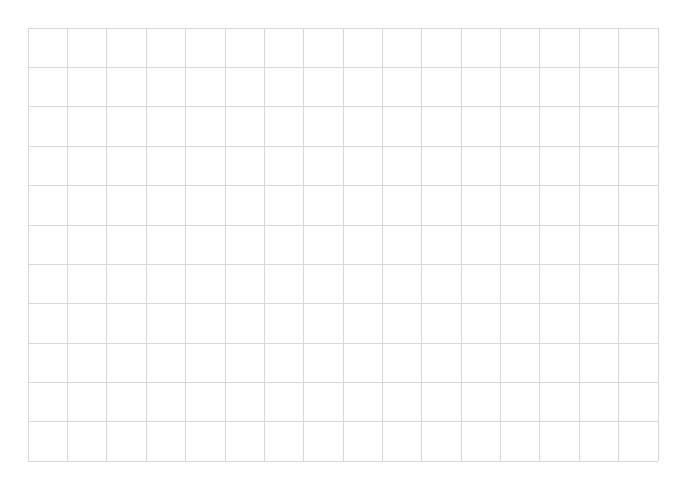
\begin{tikzpicture}
\draw[step=2*\unitsize,gray!30,very thin,shift={(-\unitsize, -\unitsize)}] (-6.0*\unitsize,-6.0*\unitsize) grid (26.0*\unitsize,16.0*\unitsize);
\end{tikzpicture}
}
\end{center}

We fix part of the $\mathbb{Z}^2$ grid as the board on which Morpion Solitiare is played.

\end{frame}

\begin{frame}
\frametitle{Vocabulary}

\begin{itemize}
\item Dot, $d = (x,y)$. Let $\mathcal{D}$ denote set of all (possible) dots on the board.

\vspace{1mm}
\item Segment,  $s = \{ d_1, d_2 \}$ with $d_1, d_2$ adjacent dots. Let $\mathcal{S}$ denote set of all (possible) segments on the board.

\vspace{2mm}
\begin{center}
\scalebox{0.7}{
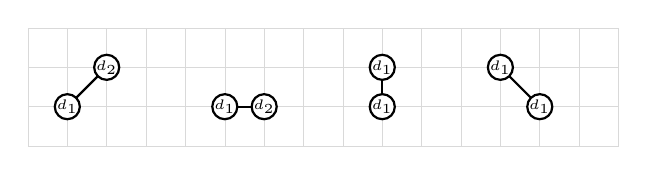
\begin{tikzpicture}[scale=2]
\draw[step=\unitsize,gray!30,very thin] (0*\unitsize,0*\unitsize) grid (15.00000*\unitsize,3.00000*\unitsize);
\tikzstyle{every node}=[draw,
                        circle,
                        fill=white,
                        minimum size  = 1.2*\unitsize,
                        node distance = 2*\unitsize,
                        inner sep=0pt,
                        font=\tiny
                        ]
\draw[thick] (1*\unitsize,1*\unitsize) node {$d_1$} -- (2*\unitsize,2*\unitsize) node {$d_2$};
\draw[thick] (5*\unitsize,1*\unitsize) node {$d_1$} -- (6*\unitsize,1*\unitsize) node {$d_2$};
\draw[thick] (9*\unitsize,1*\unitsize) node {$d_1$} -- (9*\unitsize,2*\unitsize) node {$d_1$};
\draw[thick] (12*\unitsize,2*\unitsize) node {$d_1$} -- (13*\unitsize,1*\unitsize) node {$d_1$};
\end{tikzpicture}
}
\end{center}

\vspace{1mm}
\item Move,  $m = \{ \{ d_1, d_2 \}, \{ d_2, d_3 \}, \{ d_3, d_4 \}, \{ d_4, d_5 \} \}$. Let $\mathcal{M}$ denote set of all (possible) moves on the board.

\vspace{2mm}
\begin{center}
\scalebox{0.7}{
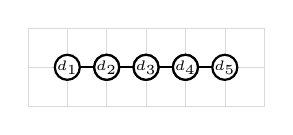
\begin{tikzpicture}[scale=2]
\draw[step=\unitsize,gray!30,very thin] (0*\unitsize,0*\unitsize) grid (6.00000*\unitsize,2.00000*\unitsize);
\tikzstyle{every node}=[draw,
                        circle,
                        fill=white,
                        minimum size  = 1.2*\unitsize,
                        node distance = 2*\unitsize,
                        inner sep=0pt,
                        font=\tiny
                        ]
\draw[thick] (1*\unitsize,1*\unitsize) node {$d_1$} -- (2*\unitsize,1*\unitsize) node {$d_2$};
\draw[thick] (2*\unitsize,1*\unitsize) node {$d_2$} -- (3*\unitsize,1*\unitsize) node {$d_3$};
\draw[thick] (3*\unitsize,1*\unitsize) node {$d_3$} -- (4*\unitsize,1*\unitsize) node {$d_4$};
\draw[thick] (4*\unitsize,1*\unitsize) node {$d_4$} -- (5*\unitsize,1*\unitsize) node {$d_5$};
\end{tikzpicture}
}
\end{center}

\end{itemize}

\end{frame}

\begin{frame}
\frametitle{Morpion position graph}

For each dot $d$ on board we define a binary variable $\dt_d$.

For each move $m$ on board we define a binary variable $\mv_m$.

\vspace*{-7mm}
\begin{center}
  
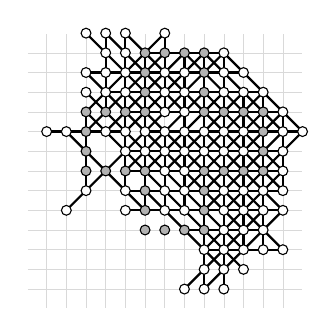
\begin{tikzpicture}[scale=0.5]
\draw[step=2*\unitsize,gray!30,very thin,shift={(-\unitsize, -\unitsize)}] (-13.900000*\unitsize,-15.900000*\unitsize) grid (13.900000*\unitsize,11.900000*\unitsize);
\tikzstyle{every node}=[draw,
			circle,
			fill=white,
			minimum size  = 0.5*\unitsize,
			node distance = 2*\unitsize,
			inner sep=0pt
			] 


\draw[thick] (-9*\unitsize,-1*\unitsize) -- (-9*\unitsize,1*\unitsize);
    

\draw[thick] (-9*\unitsize,1*\unitsize) -- (-9*\unitsize,3*\unitsize);
    

\draw[thick] (-9*\unitsize,-1*\unitsize) -- (-9*\unitsize,-3*\unitsize);
    

\draw[thick] (-9*\unitsize,-3*\unitsize) -- (-9*\unitsize,-5*\unitsize);
    

\draw[thick] (-5*\unitsize,5*\unitsize) -- (-3*\unitsize,7*\unitsize);
    

\draw[thick] (-3*\unitsize,7*\unitsize) -- (-1*\unitsize,9*\unitsize);
    

\draw[thick] (-5*\unitsize,5*\unitsize) -- (-7*\unitsize,3*\unitsize);
    

\draw[thick] (-7*\unitsize,3*\unitsize) -- (-9*\unitsize,1*\unitsize);
    

\draw[thick] (-3*\unitsize,5*\unitsize) -- (-3*\unitsize,7*\unitsize);
    

\draw[thick] (-3*\unitsize,7*\unitsize) -- (-3*\unitsize,9*\unitsize);
    

\draw[thick] (-3*\unitsize,5*\unitsize) -- (-3*\unitsize,3*\unitsize);
    

\draw[thick] (-3*\unitsize,3*\unitsize) -- (-3*\unitsize,1*\unitsize);
    

\draw[thick] (3*\unitsize,5*\unitsize) -- (3*\unitsize,7*\unitsize);
    

\draw[thick] (3*\unitsize,7*\unitsize) -- (3*\unitsize,9*\unitsize);
    

\draw[thick] (3*\unitsize,5*\unitsize) -- (3*\unitsize,3*\unitsize);
    

\draw[thick] (3*\unitsize,3*\unitsize) -- (3*\unitsize,1*\unitsize);
    

\draw[thick] (5*\unitsize,5*\unitsize) -- (7*\unitsize,3*\unitsize);
    

\draw[thick] (7*\unitsize,3*\unitsize) -- (9*\unitsize,1*\unitsize);
    

\draw[thick] (5*\unitsize,5*\unitsize) -- (3*\unitsize,7*\unitsize);
    

\draw[thick] (3*\unitsize,7*\unitsize) -- (1*\unitsize,9*\unitsize);
    

\draw[thick] (1*\unitsize,9*\unitsize) -- (3*\unitsize,9*\unitsize);
    

\draw[thick] (3*\unitsize,9*\unitsize) -- (5*\unitsize,9*\unitsize);
    

\draw[thick] (1*\unitsize,9*\unitsize) -- (-1*\unitsize,9*\unitsize);
    

\draw[thick] (-1*\unitsize,9*\unitsize) -- (-3*\unitsize,9*\unitsize);
    

\draw[thick] (9*\unitsize,1*\unitsize) -- (9*\unitsize,3*\unitsize);
    

\draw[thick] (9*\unitsize,3*\unitsize) -- (9*\unitsize,5*\unitsize);
    

\draw[thick] (9*\unitsize,1*\unitsize) -- (9*\unitsize,-1*\unitsize);
    

\draw[thick] (9*\unitsize,-1*\unitsize) -- (9*\unitsize,-3*\unitsize);
    

\draw[thick] (7*\unitsize,-3*\unitsize) -- (9*\unitsize,-3*\unitsize);
    

\draw[thick] (9*\unitsize,-3*\unitsize) -- (11*\unitsize,-3*\unitsize);
    

\draw[thick] (7*\unitsize,-3*\unitsize) -- (5*\unitsize,-3*\unitsize);
    

\draw[thick] (5*\unitsize,-3*\unitsize) -- (3*\unitsize,-3*\unitsize);
    

\draw[thick] (7*\unitsize,3*\unitsize) -- (9*\unitsize,3*\unitsize);
    

\draw[thick] (9*\unitsize,3*\unitsize) -- (11*\unitsize,3*\unitsize);
    

\draw[thick] (7*\unitsize,3*\unitsize) -- (5*\unitsize,3*\unitsize);
    

\draw[thick] (5*\unitsize,3*\unitsize) -- (3*\unitsize,3*\unitsize);
    

\draw[thick] (-3*\unitsize,-3*\unitsize) -- (-3*\unitsize,-1*\unitsize);
    

\draw[thick] (-3*\unitsize,-1*\unitsize) -- (-3*\unitsize,1*\unitsize);
    

\draw[thick] (-3*\unitsize,-3*\unitsize) -- (-3*\unitsize,-5*\unitsize);
    

\draw[thick] (-3*\unitsize,-5*\unitsize) -- (-3*\unitsize,-7*\unitsize);
    

\draw[thick] (3*\unitsize,-3*\unitsize) -- (3*\unitsize,-1*\unitsize);
    

\draw[thick] (3*\unitsize,-1*\unitsize) -- (3*\unitsize,1*\unitsize);
    

\draw[thick] (3*\unitsize,-3*\unitsize) -- (3*\unitsize,-5*\unitsize);
    

\draw[thick] (3*\unitsize,-5*\unitsize) -- (3*\unitsize,-7*\unitsize);
    

\draw[thick] (7*\unitsize,-1*\unitsize) -- (9*\unitsize,1*\unitsize);
    

\draw[thick] (9*\unitsize,1*\unitsize) -- (11*\unitsize,3*\unitsize);
    

\draw[thick] (7*\unitsize,-1*\unitsize) -- (5*\unitsize,-3*\unitsize);
    

\draw[thick] (5*\unitsize,-3*\unitsize) -- (3*\unitsize,-5*\unitsize);
    

\draw[thick] (7*\unitsize,1*\unitsize) -- (9*\unitsize,-1*\unitsize);
    

\draw[thick] (9*\unitsize,-1*\unitsize) -- (11*\unitsize,-3*\unitsize);
    

\draw[thick] (7*\unitsize,1*\unitsize) -- (5*\unitsize,3*\unitsize);
    

\draw[thick] (5*\unitsize,3*\unitsize) -- (3*\unitsize,5*\unitsize);
    

\draw[thick] (7*\unitsize,1*\unitsize) -- (7*\unitsize,3*\unitsize);
    

\draw[thick] (7*\unitsize,3*\unitsize) -- (7*\unitsize,5*\unitsize);
    

\draw[thick] (7*\unitsize,1*\unitsize) -- (7*\unitsize,-1*\unitsize);
    

\draw[thick] (7*\unitsize,-1*\unitsize) -- (7*\unitsize,-3*\unitsize);
    

\draw[thick] (5*\unitsize,5*\unitsize) -- (7*\unitsize,5*\unitsize);
    

\draw[thick] (7*\unitsize,5*\unitsize) -- (9*\unitsize,5*\unitsize);
    

\draw[thick] (5*\unitsize,5*\unitsize) -- (3*\unitsize,5*\unitsize);
    

\draw[thick] (3*\unitsize,5*\unitsize) -- (1*\unitsize,5*\unitsize);
    

\draw[thick] (1*\unitsize,5*\unitsize) -- (3*\unitsize,7*\unitsize);
    

\draw[thick] (3*\unitsize,7*\unitsize) -- (5*\unitsize,9*\unitsize);
    

\draw[thick] (1*\unitsize,5*\unitsize) -- (-1*\unitsize,3*\unitsize);
    

\draw[thick] (-1*\unitsize,3*\unitsize) -- (-3*\unitsize,1*\unitsize);
    

\draw[thick] (-1*\unitsize,3*\unitsize) -- (1*\unitsize,3*\unitsize);
    

\draw[thick] (1*\unitsize,3*\unitsize) -- (3*\unitsize,3*\unitsize);
    

\draw[thick] (-1*\unitsize,3*\unitsize) -- (-3*\unitsize,3*\unitsize);
    

\draw[thick] (-3*\unitsize,3*\unitsize) -- (-5*\unitsize,3*\unitsize);
    

\draw[thick] (-1*\unitsize,1*\unitsize) -- (1*\unitsize,3*\unitsize);
    

\draw[thick] (1*\unitsize,3*\unitsize) -- (3*\unitsize,5*\unitsize);
    

\draw[thick] (-1*\unitsize,1*\unitsize) -- (-3*\unitsize,-1*\unitsize);
    

\draw[thick] (-3*\unitsize,-1*\unitsize) -- (-5*\unitsize,-3*\unitsize);
    

\draw[thick] (-1*\unitsize,1*\unitsize) -- (1*\unitsize,-1*\unitsize);
    

\draw[thick] (1*\unitsize,-1*\unitsize) -- (3*\unitsize,-3*\unitsize);
    

\draw[thick] (-1*\unitsize,1*\unitsize) -- (-3*\unitsize,3*\unitsize);
    

\draw[thick] (-3*\unitsize,3*\unitsize) -- (-5*\unitsize,5*\unitsize);
    

\draw[thick] (3*\unitsize,1*\unitsize) -- (5*\unitsize,3*\unitsize);
    

\draw[thick] (5*\unitsize,3*\unitsize) -- (7*\unitsize,5*\unitsize);
    

\draw[thick] (3*\unitsize,1*\unitsize) -- (1*\unitsize,-1*\unitsize);
    

\draw[thick] (1*\unitsize,-1*\unitsize) -- (-1*\unitsize,-3*\unitsize);
    

\draw[thick] (-1*\unitsize,-3*\unitsize) -- (1*\unitsize,-3*\unitsize);
    

\draw[thick] (1*\unitsize,-3*\unitsize) -- (3*\unitsize,-3*\unitsize);
    

\draw[thick] (-1*\unitsize,-3*\unitsize) -- (-3*\unitsize,-3*\unitsize);
    

\draw[thick] (-3*\unitsize,-3*\unitsize) -- (-5*\unitsize,-3*\unitsize);
    

\draw[thick] (5*\unitsize,1*\unitsize) -- (7*\unitsize,3*\unitsize);
    

\draw[thick] (7*\unitsize,3*\unitsize) -- (9*\unitsize,5*\unitsize);
    

\draw[thick] (5*\unitsize,1*\unitsize) -- (3*\unitsize,-1*\unitsize);
    

\draw[thick] (3*\unitsize,-1*\unitsize) -- (1*\unitsize,-3*\unitsize);
    

\draw[thick] (1*\unitsize,1*\unitsize) -- (3*\unitsize,1*\unitsize);
    

\draw[thick] (3*\unitsize,1*\unitsize) -- (5*\unitsize,1*\unitsize);
    

\draw[thick] (1*\unitsize,1*\unitsize) -- (-1*\unitsize,1*\unitsize);
    

\draw[thick] (-1*\unitsize,1*\unitsize) -- (-3*\unitsize,1*\unitsize);
    

\draw[thick] (5*\unitsize,5*\unitsize) -- (5*\unitsize,7*\unitsize);
    

\draw[thick] (5*\unitsize,7*\unitsize) -- (5*\unitsize,9*\unitsize);
    

\draw[thick] (5*\unitsize,5*\unitsize) -- (5*\unitsize,3*\unitsize);
    

\draw[thick] (5*\unitsize,3*\unitsize) -- (5*\unitsize,1*\unitsize);
    

\draw[thick] (7*\unitsize,-1*\unitsize) -- (9*\unitsize,-3*\unitsize);
    

\draw[thick] (9*\unitsize,-3*\unitsize) -- (11*\unitsize,-5*\unitsize);
    

\draw[thick] (7*\unitsize,-1*\unitsize) -- (5*\unitsize,1*\unitsize);
    

\draw[thick] (5*\unitsize,1*\unitsize) -- (3*\unitsize,3*\unitsize);
    

\draw[thick] (1*\unitsize,1*\unitsize) -- (3*\unitsize,3*\unitsize);
    

\draw[thick] (3*\unitsize,3*\unitsize) -- (5*\unitsize,5*\unitsize);
    

\draw[thick] (1*\unitsize,1*\unitsize) -- (-1*\unitsize,-1*\unitsize);
    

\draw[thick] (-1*\unitsize,-1*\unitsize) -- (-3*\unitsize,-3*\unitsize);
    

\draw[thick] (1*\unitsize,5*\unitsize) -- (1*\unitsize,7*\unitsize);
    

\draw[thick] (1*\unitsize,7*\unitsize) -- (1*\unitsize,9*\unitsize);
    

\draw[thick] (1*\unitsize,5*\unitsize) -- (1*\unitsize,3*\unitsize);
    

\draw[thick] (1*\unitsize,3*\unitsize) -- (1*\unitsize,1*\unitsize);
    

\draw[thick] (7*\unitsize,5*\unitsize) -- (9*\unitsize,3*\unitsize);
    

\draw[thick] (9*\unitsize,3*\unitsize) -- (11*\unitsize,1*\unitsize);
    

\draw[thick] (7*\unitsize,5*\unitsize) -- (5*\unitsize,7*\unitsize);
    

\draw[thick] (5*\unitsize,7*\unitsize) -- (3*\unitsize,9*\unitsize);
    

\draw[thick] (-1*\unitsize,-1*\unitsize) -- (1*\unitsize,-1*\unitsize);
    

\draw[thick] (1*\unitsize,-1*\unitsize) -- (3*\unitsize,-1*\unitsize);
    

\draw[thick] (-1*\unitsize,-1*\unitsize) -- (-3*\unitsize,-1*\unitsize);
    

\draw[thick] (-3*\unitsize,-1*\unitsize) -- (-5*\unitsize,-1*\unitsize);
    

\draw[thick] (7*\unitsize,-3*\unitsize) -- (9*\unitsize,-1*\unitsize);
    

\draw[thick] (9*\unitsize,-1*\unitsize) -- (11*\unitsize,1*\unitsize);
    

\draw[thick] (7*\unitsize,-3*\unitsize) -- (5*\unitsize,-5*\unitsize);
    

\draw[thick] (5*\unitsize,-5*\unitsize) -- (3*\unitsize,-7*\unitsize);
    

\draw[thick] (11*\unitsize,-1*\unitsize) -- (11*\unitsize,1*\unitsize);
    

\draw[thick] (11*\unitsize,1*\unitsize) -- (11*\unitsize,3*\unitsize);
    

\draw[thick] (11*\unitsize,-1*\unitsize) -- (11*\unitsize,-3*\unitsize);
    

\draw[thick] (11*\unitsize,-3*\unitsize) -- (11*\unitsize,-5*\unitsize);
    

\draw[thick] (9*\unitsize,1*\unitsize) -- (11*\unitsize,1*\unitsize);
    

\draw[thick] (11*\unitsize,1*\unitsize) -- (13*\unitsize,1*\unitsize);
    

\draw[thick] (9*\unitsize,1*\unitsize) -- (7*\unitsize,1*\unitsize);
    

\draw[thick] (7*\unitsize,1*\unitsize) -- (5*\unitsize,1*\unitsize);
    

\draw[thick] (-7*\unitsize,-3*\unitsize) -- (-5*\unitsize,-1*\unitsize);
    

\draw[thick] (-5*\unitsize,-1*\unitsize) -- (-3*\unitsize,1*\unitsize);
    

\draw[thick] (-7*\unitsize,-3*\unitsize) -- (-9*\unitsize,-5*\unitsize);
    

\draw[thick] (-9*\unitsize,-5*\unitsize) -- (-11*\unitsize,-7*\unitsize);
    

\draw[thick] (7*\unitsize,-1*\unitsize) -- (9*\unitsize,-1*\unitsize);
    

\draw[thick] (9*\unitsize,-1*\unitsize) -- (11*\unitsize,-1*\unitsize);
    

\draw[thick] (7*\unitsize,-1*\unitsize) -- (5*\unitsize,-1*\unitsize);
    

\draw[thick] (5*\unitsize,-1*\unitsize) -- (3*\unitsize,-1*\unitsize);
    

\draw[thick] (9*\unitsize,5*\unitsize) -- (11*\unitsize,3*\unitsize);
    

\draw[thick] (11*\unitsize,3*\unitsize) -- (13*\unitsize,1*\unitsize);
    

\draw[thick] (9*\unitsize,5*\unitsize) -- (7*\unitsize,7*\unitsize);
    

\draw[thick] (7*\unitsize,7*\unitsize) -- (5*\unitsize,9*\unitsize);
    

\draw[thick] (3*\unitsize,7*\unitsize) -- (5*\unitsize,7*\unitsize);
    

\draw[thick] (5*\unitsize,7*\unitsize) -- (7*\unitsize,7*\unitsize);
    

\draw[thick] (3*\unitsize,7*\unitsize) -- (1*\unitsize,7*\unitsize);
    

\draw[thick] (1*\unitsize,7*\unitsize) -- (-1*\unitsize,7*\unitsize);
    

\draw[thick] (5*\unitsize,-1*\unitsize) -- (7*\unitsize,1*\unitsize);
    

\draw[thick] (7*\unitsize,1*\unitsize) -- (9*\unitsize,3*\unitsize);
    

\draw[thick] (5*\unitsize,-1*\unitsize) -- (3*\unitsize,-3*\unitsize);
    

\draw[thick] (3*\unitsize,-3*\unitsize) -- (1*\unitsize,-5*\unitsize);
    

\draw[thick] (5*\unitsize,-3*\unitsize) -- (5*\unitsize,-1*\unitsize);
    

\draw[thick] (5*\unitsize,-1*\unitsize) -- (5*\unitsize,1*\unitsize);
    

\draw[thick] (5*\unitsize,-3*\unitsize) -- (5*\unitsize,-5*\unitsize);
    

\draw[thick] (5*\unitsize,-5*\unitsize) -- (5*\unitsize,-7*\unitsize);
    

\draw[thick] (-3*\unitsize,5*\unitsize) -- (-1*\unitsize,7*\unitsize);
    

\draw[thick] (-1*\unitsize,7*\unitsize) -- (1*\unitsize,9*\unitsize);
    

\draw[thick] (-3*\unitsize,5*\unitsize) -- (-5*\unitsize,3*\unitsize);
    

\draw[thick] (-5*\unitsize,3*\unitsize) -- (-7*\unitsize,1*\unitsize);
    

\draw[thick] (-1*\unitsize,7*\unitsize) -- (1*\unitsize,5*\unitsize);
    

\draw[thick] (1*\unitsize,5*\unitsize) -- (3*\unitsize,3*\unitsize);
    

\draw[thick] (-1*\unitsize,7*\unitsize) -- (-3*\unitsize,9*\unitsize);
    

\draw[thick] (-3*\unitsize,9*\unitsize) -- (-5*\unitsize,11*\unitsize);
    

\draw[thick] (1*\unitsize,-3*\unitsize) -- (1*\unitsize,-1*\unitsize);
    

\draw[thick] (1*\unitsize,-1*\unitsize) -- (1*\unitsize,1*\unitsize);
    

\draw[thick] (1*\unitsize,-3*\unitsize) -- (1*\unitsize,-5*\unitsize);
    

\draw[thick] (1*\unitsize,-5*\unitsize) -- (1*\unitsize,-7*\unitsize);
    

\draw[thick] (3*\unitsize,-5*\unitsize) -- (5*\unitsize,-7*\unitsize);
    

\draw[thick] (5*\unitsize,-7*\unitsize) -- (7*\unitsize,-9*\unitsize);
    

\draw[thick] (3*\unitsize,-5*\unitsize) -- (1*\unitsize,-3*\unitsize);
    

\draw[thick] (1*\unitsize,-3*\unitsize) -- (-1*\unitsize,-1*\unitsize);
    

\draw[thick] (9*\unitsize,-3*\unitsize) -- (11*\unitsize,-1*\unitsize);
    

\draw[thick] (11*\unitsize,-1*\unitsize) -- (13*\unitsize,1*\unitsize);
    

\draw[thick] (9*\unitsize,-3*\unitsize) -- (7*\unitsize,-5*\unitsize);
    

\draw[thick] (7*\unitsize,-5*\unitsize) -- (5*\unitsize,-7*\unitsize);
    

\draw[thick] (-5*\unitsize,-1*\unitsize) -- (-3*\unitsize,-3*\unitsize);
    

\draw[thick] (-3*\unitsize,-3*\unitsize) -- (-1*\unitsize,-5*\unitsize);
    

\draw[thick] (-5*\unitsize,-1*\unitsize) -- (-7*\unitsize,1*\unitsize);
    

\draw[thick] (-7*\unitsize,1*\unitsize) -- (-9*\unitsize,3*\unitsize);
    

\draw[thick] (5*\unitsize,-3*\unitsize) -- (7*\unitsize,-5*\unitsize);
    

\draw[thick] (7*\unitsize,-5*\unitsize) -- (9*\unitsize,-7*\unitsize);
    

\draw[thick] (5*\unitsize,-3*\unitsize) -- (3*\unitsize,-1*\unitsize);
    

\draw[thick] (3*\unitsize,-1*\unitsize) -- (1*\unitsize,1*\unitsize);
    

\draw[thick] (7*\unitsize,-5*\unitsize) -- (9*\unitsize,-5*\unitsize);
    

\draw[thick] (9*\unitsize,-5*\unitsize) -- (11*\unitsize,-5*\unitsize);
    

\draw[thick] (7*\unitsize,-5*\unitsize) -- (5*\unitsize,-5*\unitsize);
    

\draw[thick] (5*\unitsize,-5*\unitsize) -- (3*\unitsize,-5*\unitsize);
    

\draw[thick] (-1*\unitsize,-5*\unitsize) -- (1*\unitsize,-5*\unitsize);
    

\draw[thick] (1*\unitsize,-5*\unitsize) -- (3*\unitsize,-5*\unitsize);
    

\draw[thick] (-1*\unitsize,-5*\unitsize) -- (-3*\unitsize,-5*\unitsize);
    

\draw[thick] (-3*\unitsize,-5*\unitsize) -- (-5*\unitsize,-5*\unitsize);
    

\draw[thick] (-1*\unitsize,-3*\unitsize) -- (-1*\unitsize,-1*\unitsize);
    

\draw[thick] (-1*\unitsize,-1*\unitsize) -- (-1*\unitsize,1*\unitsize);
    

\draw[thick] (-1*\unitsize,-3*\unitsize) -- (-1*\unitsize,-5*\unitsize);
    

\draw[thick] (-1*\unitsize,-5*\unitsize) -- (-1*\unitsize,-7*\unitsize);
    

\draw[thick] (7*\unitsize,-3*\unitsize) -- (9*\unitsize,-5*\unitsize);
    

\draw[thick] (9*\unitsize,-5*\unitsize) -- (11*\unitsize,-7*\unitsize);
    

\draw[thick] (7*\unitsize,-3*\unitsize) -- (5*\unitsize,-1*\unitsize);
    

\draw[thick] (5*\unitsize,-1*\unitsize) -- (3*\unitsize,1*\unitsize);
    

\draw[thick] (-7*\unitsize,-3*\unitsize) -- (-5*\unitsize,-5*\unitsize);
    

\draw[thick] (-5*\unitsize,-5*\unitsize) -- (-3*\unitsize,-7*\unitsize);
    

\draw[thick] (-7*\unitsize,-3*\unitsize) -- (-9*\unitsize,-1*\unitsize);
    

\draw[thick] (-9*\unitsize,-1*\unitsize) -- (-11*\unitsize,1*\unitsize);
    

\draw[thick] (-1*\unitsize,-7*\unitsize) -- (1*\unitsize,-7*\unitsize);
    

\draw[thick] (1*\unitsize,-7*\unitsize) -- (3*\unitsize,-7*\unitsize);
    

\draw[thick] (-1*\unitsize,-7*\unitsize) -- (-3*\unitsize,-7*\unitsize);
    

\draw[thick] (-3*\unitsize,-7*\unitsize) -- (-5*\unitsize,-7*\unitsize);
    

\draw[thick] (-5*\unitsize,-1*\unitsize) -- (-5*\unitsize,1*\unitsize);
    

\draw[thick] (-5*\unitsize,1*\unitsize) -- (-5*\unitsize,3*\unitsize);
    

\draw[thick] (-5*\unitsize,-1*\unitsize) -- (-5*\unitsize,-3*\unitsize);
    

\draw[thick] (-5*\unitsize,-3*\unitsize) -- (-5*\unitsize,-5*\unitsize);
    

\draw[thick] (7*\unitsize,-7*\unitsize) -- (9*\unitsize,-7*\unitsize);
    

\draw[thick] (9*\unitsize,-7*\unitsize) -- (11*\unitsize,-7*\unitsize);
    

\draw[thick] (7*\unitsize,-7*\unitsize) -- (5*\unitsize,-7*\unitsize);
    

\draw[thick] (5*\unitsize,-7*\unitsize) -- (3*\unitsize,-7*\unitsize);
    

\draw[thick] (-9*\unitsize,1*\unitsize) -- (-7*\unitsize,1*\unitsize);
    

\draw[thick] (-7*\unitsize,1*\unitsize) -- (-5*\unitsize,1*\unitsize);
    

\draw[thick] (-9*\unitsize,1*\unitsize) -- (-11*\unitsize,1*\unitsize);
    

\draw[thick] (-11*\unitsize,1*\unitsize) -- (-13*\unitsize,1*\unitsize);
    

\draw[thick] (-5*\unitsize,1*\unitsize) -- (-3*\unitsize,-1*\unitsize);
    

\draw[thick] (-3*\unitsize,-1*\unitsize) -- (-1*\unitsize,-3*\unitsize);
    

\draw[thick] (-5*\unitsize,1*\unitsize) -- (-7*\unitsize,3*\unitsize);
    

\draw[thick] (-7*\unitsize,3*\unitsize) -- (-9*\unitsize,5*\unitsize);
    

\draw[thick] (-1*\unitsize,5*\unitsize) -- (1*\unitsize,7*\unitsize);
    

\draw[thick] (1*\unitsize,7*\unitsize) -- (3*\unitsize,9*\unitsize);
    

\draw[thick] (-1*\unitsize,5*\unitsize) -- (-3*\unitsize,3*\unitsize);
    

\draw[thick] (-3*\unitsize,3*\unitsize) -- (-5*\unitsize,1*\unitsize);
    

\draw[thick] (7*\unitsize,-7*\unitsize) -- (7*\unitsize,-5*\unitsize);
    

\draw[thick] (7*\unitsize,-5*\unitsize) -- (7*\unitsize,-3*\unitsize);
    

\draw[thick] (7*\unitsize,-7*\unitsize) -- (7*\unitsize,-9*\unitsize);
    

\draw[thick] (7*\unitsize,-9*\unitsize) -- (7*\unitsize,-11*\unitsize);
    

\draw[thick] (-3*\unitsize,5*\unitsize) -- (-1*\unitsize,5*\unitsize);
    

\draw[thick] (-1*\unitsize,5*\unitsize) -- (1*\unitsize,5*\unitsize);
    

\draw[thick] (-3*\unitsize,5*\unitsize) -- (-5*\unitsize,5*\unitsize);
    

\draw[thick] (-5*\unitsize,5*\unitsize) -- (-7*\unitsize,5*\unitsize);
    

\draw[thick] (-1*\unitsize,7*\unitsize) -- (-1*\unitsize,9*\unitsize);
    

\draw[thick] (-1*\unitsize,9*\unitsize) -- (-1*\unitsize,11*\unitsize);
    

\draw[thick] (-1*\unitsize,7*\unitsize) -- (-1*\unitsize,5*\unitsize);
    

\draw[thick] (-1*\unitsize,5*\unitsize) -- (-1*\unitsize,3*\unitsize);
    

\draw[thick] (3*\unitsize,-7*\unitsize) -- (5*\unitsize,-9*\unitsize);
    

\draw[thick] (5*\unitsize,-9*\unitsize) -- (7*\unitsize,-11*\unitsize);
    

\draw[thick] (3*\unitsize,-7*\unitsize) -- (1*\unitsize,-5*\unitsize);
    

\draw[thick] (1*\unitsize,-5*\unitsize) -- (-1*\unitsize,-3*\unitsize);
    

\draw[thick] (-5*\unitsize,3*\unitsize) -- (-3*\unitsize,1*\unitsize);
    

\draw[thick] (-3*\unitsize,1*\unitsize) -- (-1*\unitsize,-1*\unitsize);
    

\draw[thick] (-5*\unitsize,3*\unitsize) -- (-7*\unitsize,5*\unitsize);
    

\draw[thick] (-7*\unitsize,5*\unitsize) -- (-9*\unitsize,7*\unitsize);
    

\draw[thick] (-5*\unitsize,7*\unitsize) -- (-3*\unitsize,9*\unitsize);
    

\draw[thick] (-3*\unitsize,9*\unitsize) -- (-1*\unitsize,11*\unitsize);
    

\draw[thick] (-5*\unitsize,7*\unitsize) -- (-7*\unitsize,5*\unitsize);
    

\draw[thick] (-7*\unitsize,5*\unitsize) -- (-9*\unitsize,3*\unitsize);
    

\draw[thick] (7*\unitsize,-7*\unitsize) -- (9*\unitsize,-5*\unitsize);
    

\draw[thick] (9*\unitsize,-5*\unitsize) -- (11*\unitsize,-3*\unitsize);
    

\draw[thick] (7*\unitsize,-7*\unitsize) -- (5*\unitsize,-9*\unitsize);
    

\draw[thick] (5*\unitsize,-9*\unitsize) -- (3*\unitsize,-11*\unitsize);
    

\draw[thick] (5*\unitsize,-9*\unitsize) -- (7*\unitsize,-9*\unitsize);
    

\draw[thick] (7*\unitsize,-9*\unitsize) -- (9*\unitsize,-9*\unitsize);
    

\draw[thick] (5*\unitsize,-9*\unitsize) -- (3*\unitsize,-9*\unitsize);
    

\draw[thick] (3*\unitsize,-9*\unitsize) -- (1*\unitsize,-9*\unitsize);
    

\draw[thick] (-5*\unitsize,7*\unitsize) -- (-3*\unitsize,7*\unitsize);
    

\draw[thick] (-3*\unitsize,7*\unitsize) -- (-1*\unitsize,7*\unitsize);
    

\draw[thick] (-5*\unitsize,7*\unitsize) -- (-7*\unitsize,7*\unitsize);
    

\draw[thick] (-7*\unitsize,7*\unitsize) -- (-9*\unitsize,7*\unitsize);
    

\draw[thick] (-5*\unitsize,7*\unitsize) -- (-5*\unitsize,9*\unitsize);
    

\draw[thick] (-5*\unitsize,9*\unitsize) -- (-5*\unitsize,11*\unitsize);
    

\draw[thick] (-5*\unitsize,7*\unitsize) -- (-5*\unitsize,5*\unitsize);
    

\draw[thick] (-5*\unitsize,5*\unitsize) -- (-5*\unitsize,3*\unitsize);
    

\draw[thick] (1*\unitsize,-9*\unitsize) -- (3*\unitsize,-11*\unitsize);
    

\draw[thick] (3*\unitsize,-11*\unitsize) -- (5*\unitsize,-13*\unitsize);
    

\draw[thick] (1*\unitsize,-9*\unitsize) -- (-1*\unitsize,-7*\unitsize);
    

\draw[thick] (-1*\unitsize,-7*\unitsize) -- (-3*\unitsize,-5*\unitsize);
    

\draw[thick] (9*\unitsize,-7*\unitsize) -- (9*\unitsize,-5*\unitsize);
    

\draw[thick] (9*\unitsize,-5*\unitsize) -- (9*\unitsize,-3*\unitsize);
    

\draw[thick] (9*\unitsize,-7*\unitsize) -- (9*\unitsize,-9*\unitsize);
    

\draw[thick] (9*\unitsize,-9*\unitsize) -- (9*\unitsize,-11*\unitsize);
    

\draw[thick] (7*\unitsize,-7*\unitsize) -- (9*\unitsize,-9*\unitsize);
    

\draw[thick] (9*\unitsize,-9*\unitsize) -- (11*\unitsize,-11*\unitsize);
    

\draw[thick] (7*\unitsize,-7*\unitsize) -- (5*\unitsize,-5*\unitsize);
    

\draw[thick] (5*\unitsize,-5*\unitsize) -- (3*\unitsize,-3*\unitsize);
    

\draw[thick] (-3*\unitsize,7*\unitsize) -- (-1*\unitsize,5*\unitsize);
    

\draw[thick] (-1*\unitsize,5*\unitsize) -- (1*\unitsize,3*\unitsize);
    

\draw[thick] (-3*\unitsize,7*\unitsize) -- (-5*\unitsize,9*\unitsize);
    

\draw[thick] (-5*\unitsize,9*\unitsize) -- (-7*\unitsize,11*\unitsize);
    

\draw[thick] (7*\unitsize,-11*\unitsize) -- (9*\unitsize,-9*\unitsize);
    

\draw[thick] (9*\unitsize,-9*\unitsize) -- (11*\unitsize,-7*\unitsize);
    

\draw[thick] (7*\unitsize,-11*\unitsize) -- (5*\unitsize,-13*\unitsize);
    

\draw[thick] (5*\unitsize,-13*\unitsize) -- (3*\unitsize,-15*\unitsize);
    

\draw[thick] (7*\unitsize,-11*\unitsize) -- (9*\unitsize,-11*\unitsize);
    

\draw[thick] (9*\unitsize,-11*\unitsize) -- (11*\unitsize,-11*\unitsize);
    

\draw[thick] (7*\unitsize,-11*\unitsize) -- (5*\unitsize,-11*\unitsize);
    

\draw[thick] (5*\unitsize,-11*\unitsize) -- (3*\unitsize,-11*\unitsize);
    

\draw[thick] (-7*\unitsize,7*\unitsize) -- (-7*\unitsize,9*\unitsize);
    

\draw[thick] (-7*\unitsize,9*\unitsize) -- (-7*\unitsize,11*\unitsize);
    

\draw[thick] (-7*\unitsize,7*\unitsize) -- (-7*\unitsize,5*\unitsize);
    

\draw[thick] (-7*\unitsize,5*\unitsize) -- (-7*\unitsize,3*\unitsize);
    

\draw[thick] (3*\unitsize,-11*\unitsize) -- (3*\unitsize,-9*\unitsize);
    

\draw[thick] (3*\unitsize,-9*\unitsize) -- (3*\unitsize,-7*\unitsize);
    

\draw[thick] (3*\unitsize,-11*\unitsize) -- (3*\unitsize,-13*\unitsize);
    

\draw[thick] (3*\unitsize,-13*\unitsize) -- (3*\unitsize,-15*\unitsize);
    

\draw[thick] (5*\unitsize,-11*\unitsize) -- (5*\unitsize,-9*\unitsize);
    

\draw[thick] (5*\unitsize,-9*\unitsize) -- (5*\unitsize,-7*\unitsize);
    

\draw[thick] (5*\unitsize,-11*\unitsize) -- (5*\unitsize,-13*\unitsize);
    

\draw[thick] (5*\unitsize,-13*\unitsize) -- (5*\unitsize,-15*\unitsize);
    

\draw[thick] (3*\unitsize,-9*\unitsize) -- (5*\unitsize,-11*\unitsize);
    

\draw[thick] (5*\unitsize,-11*\unitsize) -- (7*\unitsize,-13*\unitsize);
    

\draw[thick] (3*\unitsize,-9*\unitsize) -- (1*\unitsize,-7*\unitsize);
    

\draw[thick] (1*\unitsize,-7*\unitsize) -- (-1*\unitsize,-5*\unitsize);
    

\draw[thick] (-5*\unitsize,7*\unitsize) -- (-3*\unitsize,5*\unitsize);
    

\draw[thick] (-3*\unitsize,5*\unitsize) -- (-1*\unitsize,3*\unitsize);
    

\draw[thick] (-5*\unitsize,7*\unitsize) -- (-7*\unitsize,9*\unitsize);
    

\draw[thick] (-7*\unitsize,9*\unitsize) -- (-9*\unitsize,11*\unitsize);
    

\draw[thick] (5*\unitsize,-11*\unitsize) -- (7*\unitsize,-9*\unitsize);
    

\draw[thick] (7*\unitsize,-9*\unitsize) -- (9*\unitsize,-7*\unitsize);
    

\draw[thick] (5*\unitsize,-11*\unitsize) -- (3*\unitsize,-13*\unitsize);
    

\draw[thick] (3*\unitsize,-13*\unitsize) -- (1*\unitsize,-15*\unitsize);
    

\node[fill=black!30, thin] at (3*\unitsize,9*\unitsize) {};
        

\node[fill=black!30, thin] at (3*\unitsize,7*\unitsize) {};
        

\node[fill=black!30, thin] at (3*\unitsize,5*\unitsize) {};
        

\node[fill=black!30, thin] at (3*\unitsize,3*\unitsize) {};
        

\node[fill=black!30, thin] at (5*\unitsize,3*\unitsize) {};
        

\node[fill=black!30, thin] at (7*\unitsize,3*\unitsize) {};
        

\node[fill=black!30, thin] at (9*\unitsize,3*\unitsize) {};
        

\node[fill=black!30, thin] at (9*\unitsize,1*\unitsize) {};
        

\node[fill=black!30, thin] at (9*\unitsize,-1*\unitsize) {};
        

\node[fill=black!30, thin] at (9*\unitsize,-3*\unitsize) {};
        

\node[fill=black!30, thin] at (7*\unitsize,-3*\unitsize) {};
        

\node[fill=black!30, thin] at (5*\unitsize,-3*\unitsize) {};
        

\node[fill=black!30, thin] at (3*\unitsize,-3*\unitsize) {};
        

\node[fill=black!30, thin] at (3*\unitsize,-5*\unitsize) {};
        

\node[fill=black!30, thin] at (3*\unitsize,-7*\unitsize) {};
        

\node[fill=black!30, thin] at (3*\unitsize,-9*\unitsize) {};
        

\node[fill=black!30, thin] at (1*\unitsize,-9*\unitsize) {};
        

\node[fill=black!30, thin] at (-1*\unitsize,-9*\unitsize) {};
        

\node[fill=black!30, thin] at (-3*\unitsize,-9*\unitsize) {};
        

\node[fill=black!30, thin] at (-3*\unitsize,-7*\unitsize) {};
        

\node[fill=black!30, thin] at (-3*\unitsize,-5*\unitsize) {};
        

\node[fill=black!30, thin] at (-3*\unitsize,-3*\unitsize) {};
        

\node[fill=black!30, thin] at (-5*\unitsize,-3*\unitsize) {};
        

\node[fill=black!30, thin] at (-7*\unitsize,-3*\unitsize) {};
        

\node[fill=black!30, thin] at (-9*\unitsize,-3*\unitsize) {};
        

\node[fill=black!30, thin] at (-9*\unitsize,-1*\unitsize) {};
        

\node[fill=black!30, thin] at (-9*\unitsize,1*\unitsize) {};
        

\node[fill=black!30, thin] at (-9*\unitsize,3*\unitsize) {};
        

\node[fill=black!30, thin] at (-7*\unitsize,3*\unitsize) {};
        

\node[fill=black!30, thin] at (-5*\unitsize,3*\unitsize) {};
        

\node[fill=black!30, thin] at (-3*\unitsize,3*\unitsize) {};
        

\node[fill=black!30, thin] at (-3*\unitsize,5*\unitsize) {};
        

\node[fill=black!30, thin] at (-3*\unitsize,7*\unitsize) {};
        

\node[fill=black!30, thin] at (-3*\unitsize,9*\unitsize) {};
        

\node[fill=black!30, thin] at (-1*\unitsize,9*\unitsize) {};
        

\node[fill=black!30, thin] at (1*\unitsize,9*\unitsize) {};
        

\node[thin] at (-9*\unitsize,-5*\unitsize)  {\scalebox{0.35}{}};
            

\node[thin] at (-5*\unitsize,5*\unitsize)  {\scalebox{0.35}{}};
            

\node[thin] at (-3*\unitsize,1*\unitsize)  {\scalebox{0.35}{}};
            

\node[thin] at (3*\unitsize,1*\unitsize)  {\scalebox{0.35}{}};
            

\node[thin] at (5*\unitsize,5*\unitsize)  {\scalebox{0.35}{}};
            

\node[thin] at (5*\unitsize,9*\unitsize)  {\scalebox{0.35}{}};
            

\node[thin] at (9*\unitsize,5*\unitsize)  {\scalebox{0.35}{}};
            

\node[thin] at (11*\unitsize,-3*\unitsize)  {\scalebox{0.35}{}};
            

\node[thin] at (11*\unitsize,3*\unitsize)  {\scalebox{0.35}{}};
            

\node[thin] at (-3*\unitsize,-1*\unitsize)  {\scalebox{0.35}{}};
            

\node[thin] at (3*\unitsize,-1*\unitsize)  {\scalebox{0.35}{}};
            

\node[thin] at (7*\unitsize,-1*\unitsize)  {\scalebox{0.35}{}};
            

\node[thin] at (7*\unitsize,1*\unitsize)  {\scalebox{0.35}{}};
            

\node[thin] at (7*\unitsize,5*\unitsize)  {\scalebox{0.35}{}};
            

\node[thin] at (1*\unitsize,5*\unitsize)  {\scalebox{0.35}{}};
            

\node[thin] at (-1*\unitsize,3*\unitsize)  {\scalebox{0.35}{}};
            

\node[thin] at (1*\unitsize,3*\unitsize)  {\scalebox{0.35}{}};
            

\node[thin] at (-1*\unitsize,1*\unitsize)  {\scalebox{0.35}{}};
            

\node[thin] at (1*\unitsize,-1*\unitsize)  {\scalebox{0.35}{}};
            

\node[thin] at (-1*\unitsize,-3*\unitsize)  {\scalebox{0.35}{}};
            

\node[thin] at (1*\unitsize,-3*\unitsize)  {\scalebox{0.35}{}};
            

\node[thin] at (5*\unitsize,1*\unitsize)  {\scalebox{0.35}{}};
            

\node[thin] at (1*\unitsize,1*\unitsize)  {\scalebox{0.35}{}};
            

\node[thin] at (5*\unitsize,7*\unitsize)  {\scalebox{0.35}{}};
            

\node[thin] at (11*\unitsize,-5*\unitsize)  {\scalebox{0.35}{}};
            

\node[thin] at (-1*\unitsize,-1*\unitsize)  {\scalebox{0.35}{}};
            

\node[thin] at (1*\unitsize,7*\unitsize)  {\scalebox{0.35}{}};
            

\node[thin] at (11*\unitsize,1*\unitsize)  {\scalebox{0.35}{}};
            

\node[thin] at (-5*\unitsize,-1*\unitsize)  {\scalebox{0.35}{}};
            

\node[thin] at (5*\unitsize,-5*\unitsize)  {\scalebox{0.35}{}};
            

\node[thin] at (11*\unitsize,-1*\unitsize)  {\scalebox{0.35}{}};
            

\node[thin] at (13*\unitsize,1*\unitsize)  {\scalebox{0.35}{}};
            

\node[thin] at (-11*\unitsize,-7*\unitsize)  {\scalebox{0.35}{}};
            

\node[thin] at (5*\unitsize,-1*\unitsize)  {\scalebox{0.35}{}};
            

\node[thin] at (7*\unitsize,7*\unitsize)  {\scalebox{0.35}{}};
            

\node[thin] at (-1*\unitsize,7*\unitsize)  {\scalebox{0.35}{}};
            

\node[thin] at (1*\unitsize,-5*\unitsize)  {\scalebox{0.35}{}};
            

\node[thin] at (5*\unitsize,-7*\unitsize)  {\scalebox{0.35}{}};
            

\node[thin] at (-7*\unitsize,1*\unitsize)  {\scalebox{0.35}{}};
            

\node[thin] at (-5*\unitsize,11*\unitsize)  {\scalebox{0.35}{}};
            

\node[thin] at (1*\unitsize,-7*\unitsize)  {\scalebox{0.35}{}};
            

\node[thin] at (7*\unitsize,-9*\unitsize)  {\scalebox{0.35}{}};
            

\node[thin] at (7*\unitsize,-5*\unitsize)  {\scalebox{0.35}{}};
            

\node[thin] at (-1*\unitsize,-5*\unitsize)  {\scalebox{0.35}{}};
            

\node[thin] at (9*\unitsize,-7*\unitsize)  {\scalebox{0.35}{}};
            

\node[thin] at (9*\unitsize,-5*\unitsize)  {\scalebox{0.35}{}};
            

\node[thin] at (-5*\unitsize,-5*\unitsize)  {\scalebox{0.35}{}};
            

\node[thin] at (-1*\unitsize,-7*\unitsize)  {\scalebox{0.35}{}};
            

\node[thin] at (11*\unitsize,-7*\unitsize)  {\scalebox{0.35}{}};
            

\node[thin] at (-11*\unitsize,1*\unitsize)  {\scalebox{0.35}{}};
            

\node[thin] at (-5*\unitsize,-7*\unitsize)  {\scalebox{0.35}{}};
            

\node[thin] at (-5*\unitsize,1*\unitsize)  {\scalebox{0.35}{}};
            

\node[thin] at (7*\unitsize,-7*\unitsize)  {\scalebox{0.35}{}};
            

\node[thin] at (-13*\unitsize,1*\unitsize)  {\scalebox{0.35}{}};
            

\node[thin] at (-9*\unitsize,5*\unitsize)  {\scalebox{0.35}{}};
            

\node[thin] at (-1*\unitsize,5*\unitsize)  {\scalebox{0.35}{}};
            

\node[thin] at (7*\unitsize,-11*\unitsize)  {\scalebox{0.35}{}};
            

\node[thin] at (-7*\unitsize,5*\unitsize)  {\scalebox{0.35}{}};
            

\node[thin] at (-1*\unitsize,11*\unitsize)  {\scalebox{0.35}{}};
            

\node[thin] at (5*\unitsize,-9*\unitsize)  {\scalebox{0.35}{}};
            

\node[thin] at (-9*\unitsize,7*\unitsize)  {\scalebox{0.35}{}};
            

\node[thin] at (-5*\unitsize,7*\unitsize)  {\scalebox{0.35}{}};
            

\node[thin] at (3*\unitsize,-11*\unitsize)  {\scalebox{0.35}{}};
            

\node[thin] at (9*\unitsize,-9*\unitsize)  {\scalebox{0.35}{}};
            

\node[thin] at (-7*\unitsize,7*\unitsize)  {\scalebox{0.35}{}};
            

\node[thin] at (-5*\unitsize,9*\unitsize)  {\scalebox{0.35}{}};
            

\node[thin] at (5*\unitsize,-13*\unitsize)  {\scalebox{0.35}{}};
            

\node[thin] at (9*\unitsize,-11*\unitsize)  {\scalebox{0.35}{}};
            

\node[thin] at (11*\unitsize,-11*\unitsize)  {\scalebox{0.35}{}};
            

\node[thin] at (-7*\unitsize,11*\unitsize)  {\scalebox{0.35}{}};
            

\node[thin] at (3*\unitsize,-15*\unitsize)  {\scalebox{0.35}{}};
            

\node[thin] at (5*\unitsize,-11*\unitsize)  {\scalebox{0.35}{}};
            

\node[thin] at (-7*\unitsize,9*\unitsize)  {\scalebox{0.35}{}};
            

\node[thin] at (3*\unitsize,-13*\unitsize)  {\scalebox{0.35}{}};
            

\node[thin] at (5*\unitsize,-15*\unitsize)  {\scalebox{0.35}{}};
            

\node[thin] at (7*\unitsize,-13*\unitsize)  {\scalebox{0.35}{}};
            

\node[thin] at (-9*\unitsize,11*\unitsize)  {\scalebox{0.35}{}};
            

\node[thin] at (1*\unitsize,-15*\unitsize)  {\scalebox{0.35}{}};
            

\end{tikzpicture}


\end{center}

\vspace*{-7mm}
Every Morpion position graph can be encoded using these variables:
\vspace*{-4mm}
\begin{itemize}
  \item set $\dt_d$ to $1$ iff the dot is a vertex of the graph
  \item set $\mv_m$ to $1$ iff move $m$ was in the playout.
\end{itemize}

\end{frame}

\begin{frame}
\frametitle{Properties of Morpion positions}

We start with $36$ dots and every move adds $1$ dot.

\[
  36 + \sum_{m \in \mathcal{M}} \mv_m = \sum_{d \in \mathcal{D}} \dt_d.
\]

\pause\vspace{3mm}
Moves do not overlap. For each segment $s \in \mathcal{S}$:
\[
  \sum_{m \in \mathcal{M}, s \in m} \mv_m \leq 1.
\]

\pause\vspace{3mm}
We can draw a line only through dots that are placed on board.

For $m =  \{ \{ d_1, d_2 \}, \{ d_2, d_3 \}, \ldots, \{ d_4, d_5 \} \}$ and each $1 \leq i \leq 5$:
\[
   \mv_m \leq \dt_{d_i}
\]

\end{frame}

\begin{frame}
\frametitle{Linear Programming Problem}

{\bf Variable bounds.}

\[ \forall_{m \in \mathcal{M}} \mv_m \in [0, 1], \forall_{d \in \mathcal{D}}  \dt_d \in [0, 1] \]

{\bf Constraints.}

\[ 36 + \sum_{m \in \mathcal{M}} \mv_m = \sum_{d \in \mathcal{D}} \dt_d \]  
\[ \forall_{s \in \mathcal{S}} \sum_{m \in \mathcal{M}, s \in m} \mv_m \leq 1 \]
\[ \forall_{m \in \mathcal{M}, s \in m, d \in s} \mv_m \leq \dt_d \]

\vspace{2mm}
{\bf Objective.} Maximize $\displaystyle \sum_{m \in \mathcal{M}} \mv_m$.
\end{frame}

\subsection{Solutions of linear programming problem}
\begin{frame}
\frametitle{A note on solutions}

The class of graphs that can be obtained as solutions of the above MIP contain all Morpion positions on the given board.

The converse is not true.

\begin{center}
  \includegraphics[height=4cm]{positions/grid_boyer.jpg}

  \begin{flushright}
  {\tiny Grid of $317$ moves found by Ch. Boyer}
  \end{flushright}
\end{center}


\end{frame}

\begin{frame}
\frametitle{Problem of infinite board}

The objective value of the LPP strongly depends on the size of the board.

\vspace{3mm}
\begin{center}
\scalebox{0.7}{
\bgroup
\def\arraystretch{1.5}
\setlength\tabcolsep{1mm}
\begin{tabular}{|c|c|c|c|c|c|c|c|c|c|}
\hline
10 & 20 & 30 & 40 & 50 & 60 & 70 & 80 & 90 & 100 \\
\hline 64.00 & 278.50 & 619.53 & 876.55 & 1130.01 & 1387.54 & 1641.74 & 1898.13 & 2152.86 & 2408.54 \\
\hline
\end{tabular}
\egroup
}
\end{center}

\vspace{3mm}
{\footnotesize
The top row contains the length $n$ of the edge of a given square and the bottom row contains solutions to the relaxed problem on the $n\times n$ board.}

\vspace{3mm}
We need to prove that every Morpion position is containted in a board that is not too big.

\end{frame}

%%%%
%
% Isoperimetric inequality
%
%%%%

\section{Isoperimetric Inequality}
\subsection{Size of the board}

\begin{frame}[plain]

\vspace{1cm}
\centering\Huge\bf
Isoperimetric Inequality
\end{frame}

\begin{frame}
\frametitle{Area and boundary of a lattice graph}

\begin{center}
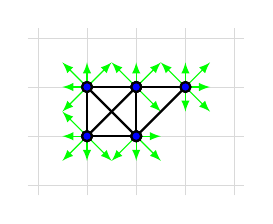
\begin{tikzpicture}[scale=2.5]
\draw[step=\unitsize,gray!30,very thin] (0.8*\unitsize,0.8*\unitsize) grid (5.20000*\unitsize,4.20000*\unitsize);
\tikzstyle{every node}=[draw,
                        circle,
                        fill=blue,
                        minimum size  = 0.5*\unitsize,
                        node distance = 2*\unitsize,
                        inner sep=0pt,
                        font=\tiny
                        ]

\draw[color=green, -latex] (2*\unitsize,2*\unitsize) -- (1.5*\unitsize,1.5*\unitsize) ;
\draw[color=green, -latex] (2*\unitsize,2*\unitsize) -- (2*\unitsize,1.5*\unitsize) ;
\draw[color=green, -latex] (2*\unitsize,2*\unitsize) -- (1.5*\unitsize,2*\unitsize) ;
\draw[color=green, -latex] (2*\unitsize,2*\unitsize) -- (1.5*\unitsize,2.5*\unitsize) ;
\draw[color=green, -latex] (2*\unitsize,2*\unitsize) -- (2.5*\unitsize,1.5*\unitsize) ;

\draw[color=green, -latex] (3*\unitsize,2*\unitsize) -- (2.5*\unitsize,1.5*\unitsize) ;
\draw[color=green, -latex] (3*\unitsize,2*\unitsize) -- (3*\unitsize,1.5*\unitsize) ;
\draw[color=green, -latex] (3*\unitsize,2*\unitsize) -- (3.5*\unitsize,1.5*\unitsize) ;
\draw[color=green, -latex] (3*\unitsize,2*\unitsize) -- (3.5*\unitsize,2*\unitsize) ;

\draw[color=green, -latex] (2*\unitsize,3*\unitsize) -- (1.5*\unitsize,3.5*\unitsize) ;
\draw[color=green, -latex] (2*\unitsize,3*\unitsize) -- (1.5*\unitsize,3*\unitsize) ;
\draw[color=green, -latex] (2*\unitsize,3*\unitsize) -- (1.5*\unitsize,2.5*\unitsize) ;
\draw[color=green, -latex] (2*\unitsize,3*\unitsize) -- (2*\unitsize,3.5*\unitsize) ;
\draw[color=green, -latex] (2*\unitsize,3*\unitsize) -- (2.5*\unitsize,3.5*\unitsize) ;

\draw[color=green, -latex] (3*\unitsize,3*\unitsize) -- (2.5*\unitsize,3.5*\unitsize) ;
\draw[color=green, -latex] (3*\unitsize,3*\unitsize) -- (3*\unitsize,3.5*\unitsize) ;
\draw[color=green, -latex] (3*\unitsize,3*\unitsize) -- (3.5*\unitsize,3.5*\unitsize) ;
\draw[color=green, -latex] (3*\unitsize,3*\unitsize) -- (3.5*\unitsize,2.5*\unitsize) ;

\draw[color=green, -latex] (4*\unitsize,3*\unitsize) -- (3.5*\unitsize,3.5*\unitsize) ;
\draw[color=green, -latex] (4*\unitsize,3*\unitsize) -- (4*\unitsize,3.5*\unitsize) ;
\draw[color=green, -latex] (4*\unitsize,3*\unitsize) -- (4*\unitsize,2.5*\unitsize) ;
\draw[color=green, -latex] (4*\unitsize,3*\unitsize) -- (4.5*\unitsize,3.5*\unitsize) ;
\draw[color=green, -latex] (4*\unitsize,3*\unitsize) -- (4.5*\unitsize,3*\unitsize) ;
\draw[color=green, -latex] (4*\unitsize,3*\unitsize) -- (4.5*\unitsize,2.5*\unitsize) ;

\draw[thick] (2*\unitsize,2*\unitsize) node {} -- (2*\unitsize,3*\unitsize) node {};
\draw[thick] (2*\unitsize,2*\unitsize) node {} -- (3*\unitsize,3*\unitsize) node {};
\draw[thick] (2*\unitsize,2*\unitsize) node {} -- (3*\unitsize,2*\unitsize) node {};
\draw[thick] (2*\unitsize,3*\unitsize) node {} -- (3*\unitsize,3*\unitsize) node {};
\draw[thick] (3*\unitsize,2*\unitsize) node {} -- (3*\unitsize,3*\unitsize) node {};
\draw[thick] (3*\unitsize,2*\unitsize) node {} -- (2*\unitsize,3*\unitsize) node {};
\draw[thick] (3*\unitsize,2*\unitsize) node {} -- (4*\unitsize,3*\unitsize) node {};
\draw[thick] (3*\unitsize,3*\unitsize) node {} -- (4*\unitsize,3*\unitsize) node {};

\end{tikzpicture}
\end{center}

The area of the graph is the number of its vertices.

\vspace{5mm}
The boundary size of the graph is the number of {\bf directed} segments with start point in a graph vertex and the endpoint in its complement.

\vspace{5mm}
Example: area $5$, boundary size $24$.

\vspace{5mm}
What we call boundary here is known in the literature as {\bf potential} (and was used by Demaine et al in their proof of the upper bound).
\end{frame}

\begin{frame}
\frametitle{Area and boundary of a lattice graph}
\begin{center}
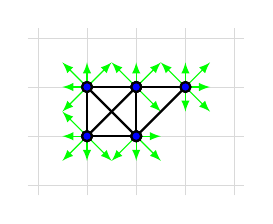
\begin{tikzpicture}[scale=2.5]
\draw[step=\unitsize,gray!30,very thin] (0.8*\unitsize,0.8*\unitsize) grid (5.20000*\unitsize,4.20000*\unitsize);
\tikzstyle{every node}=[draw,
                        circle,
                        fill=blue,
                        minimum size  = 0.5*\unitsize,
                        node distance = 2*\unitsize,
                        inner sep=0pt,
                        font=\tiny
                        ]

\draw[color=green, -latex] (2*\unitsize,2*\unitsize) -- (1.5*\unitsize,1.5*\unitsize) ;
\draw[color=green, -latex] (2*\unitsize,2*\unitsize) -- (2*\unitsize,1.5*\unitsize) ;
\draw[color=green, -latex] (2*\unitsize,2*\unitsize) -- (1.5*\unitsize,2*\unitsize) ;
\draw[color=green, -latex] (2*\unitsize,2*\unitsize) -- (1.5*\unitsize,2.5*\unitsize) ;
\draw[color=green, -latex] (2*\unitsize,2*\unitsize) -- (2.5*\unitsize,1.5*\unitsize) ;

\draw[color=green, -latex] (3*\unitsize,2*\unitsize) -- (2.5*\unitsize,1.5*\unitsize) ;
\draw[color=green, -latex] (3*\unitsize,2*\unitsize) -- (3*\unitsize,1.5*\unitsize) ;
\draw[color=green, -latex] (3*\unitsize,2*\unitsize) -- (3.5*\unitsize,1.5*\unitsize) ;
\draw[color=green, -latex] (3*\unitsize,2*\unitsize) -- (3.5*\unitsize,2*\unitsize) ;

\draw[color=green, -latex] (2*\unitsize,3*\unitsize) -- (1.5*\unitsize,3.5*\unitsize) ;
\draw[color=green, -latex] (2*\unitsize,3*\unitsize) -- (1.5*\unitsize,3*\unitsize) ;
\draw[color=green, -latex] (2*\unitsize,3*\unitsize) -- (1.5*\unitsize,2.5*\unitsize) ;
\draw[color=green, -latex] (2*\unitsize,3*\unitsize) -- (2*\unitsize,3.5*\unitsize) ;
\draw[color=green, -latex] (2*\unitsize,3*\unitsize) -- (2.5*\unitsize,3.5*\unitsize) ;

\draw[color=green, -latex] (3*\unitsize,3*\unitsize) -- (2.5*\unitsize,3.5*\unitsize) ;
\draw[color=green, -latex] (3*\unitsize,3*\unitsize) -- (3*\unitsize,3.5*\unitsize) ;
\draw[color=green, -latex] (3*\unitsize,3*\unitsize) -- (3.5*\unitsize,3.5*\unitsize) ;
\draw[color=green, -latex] (3*\unitsize,3*\unitsize) -- (3.5*\unitsize,2.5*\unitsize) ;

\draw[color=green, -latex] (4*\unitsize,3*\unitsize) -- (3.5*\unitsize,3.5*\unitsize) ;
\draw[color=green, -latex] (4*\unitsize,3*\unitsize) -- (4*\unitsize,3.5*\unitsize) ;
\draw[color=green, -latex] (4*\unitsize,3*\unitsize) -- (4*\unitsize,2.5*\unitsize) ;
\draw[color=green, -latex] (4*\unitsize,3*\unitsize) -- (4.5*\unitsize,3.5*\unitsize) ;
\draw[color=green, -latex] (4*\unitsize,3*\unitsize) -- (4.5*\unitsize,3*\unitsize) ;
\draw[color=green, -latex] (4*\unitsize,3*\unitsize) -- (4.5*\unitsize,2.5*\unitsize) ;

\draw[thick] (2*\unitsize,2*\unitsize) node {} -- (2*\unitsize,3*\unitsize) node {};
\draw[thick] (2*\unitsize,2*\unitsize) node {} -- (3*\unitsize,3*\unitsize) node {};
\draw[thick] (2*\unitsize,2*\unitsize) node {} -- (3*\unitsize,2*\unitsize) node {};
\draw[thick] (2*\unitsize,3*\unitsize) node {} -- (3*\unitsize,3*\unitsize) node {};
\draw[thick] (3*\unitsize,2*\unitsize) node {} -- (3*\unitsize,3*\unitsize) node {};
\draw[thick] (3*\unitsize,2*\unitsize) node {} -- (2*\unitsize,3*\unitsize) node {};
\draw[thick] (3*\unitsize,2*\unitsize) node {} -- (4*\unitsize,3*\unitsize) node {};
\draw[thick] (3*\unitsize,3*\unitsize) node {} -- (4*\unitsize,3*\unitsize) node {};

\end{tikzpicture}
\end{center}

  In Morpion graphs, we have the equality (boundary size is constant)
  \[
    \boundary G = 36 \cdot 8.
  \]

  In each move:
  
  \begin{itemize}
    \item draw a dot (increases area by $1$ and boundary by $8$)
    \item draw a $4$ ($8$ directed) segment line (decreases boundary by $8$)
  \end{itemize}
\end{frame}

\begin{frame}
\frametitle{Isoperimetric problem}

  We fix the length of boundary. What is the maximal possible area?
  
  \vspace{5mm}
  First step in the usual case: pass to the convex hull.

  \vspace{10mm}
  
\begin{minipage}{.48\textwidth}
  \centering
  
\begin{tikzpicture}
      \draw[color=green, thick] (0,0) -- (-1,2);
      \draw[color=green,thick] (0,0) -- (1,2);
      \draw[color=green,thick] (-1,2) -- (0,1);
      \draw[color=green,thick] (0,1) -- (1,2);
  \end{tikzpicture}  
\end{minipage}%
\begin{minipage}{.03\textwidth}
$\to$
\end{minipage}%
\begin{minipage}{.48\textwidth}
  
\begin{tikzpicture}
      \draw[color=green,thick] (0,0) -- (-1,2);
      \draw[color=green,thick] (0,0) -- (1,2);
      \draw[color=gray!60,thin] (-1,2) -- (0,1);
      \draw[color=gray!60,thin] (0,1) -- (1,2);
      \draw[color=green,thick] (-1,2) -- (1,2);
  \end{tikzpicture}  
\end{minipage}

\end{frame}

\begin{frame}
\frametitle{Octagonal hull}

\begin{figure}
\begin{minipage}{.48\textwidth}
  \centering
  
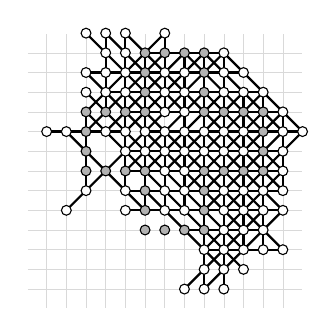
\begin{tikzpicture}[scale=0.5]
\draw[step=2*\unitsize,gray!30,very thin,shift={(-\unitsize, -\unitsize)}] (-13.900000*\unitsize,-15.900000*\unitsize) grid (13.900000*\unitsize,11.900000*\unitsize);
\tikzstyle{every node}=[draw,
			circle,
			fill=white,
			minimum size  = 0.5*\unitsize,
			node distance = 2*\unitsize,
			inner sep=0pt
			] 


\draw[thick] (-9*\unitsize,-1*\unitsize) -- (-9*\unitsize,1*\unitsize);
    

\draw[thick] (-9*\unitsize,1*\unitsize) -- (-9*\unitsize,3*\unitsize);
    

\draw[thick] (-9*\unitsize,-1*\unitsize) -- (-9*\unitsize,-3*\unitsize);
    

\draw[thick] (-9*\unitsize,-3*\unitsize) -- (-9*\unitsize,-5*\unitsize);
    

\draw[thick] (-5*\unitsize,5*\unitsize) -- (-3*\unitsize,7*\unitsize);
    

\draw[thick] (-3*\unitsize,7*\unitsize) -- (-1*\unitsize,9*\unitsize);
    

\draw[thick] (-5*\unitsize,5*\unitsize) -- (-7*\unitsize,3*\unitsize);
    

\draw[thick] (-7*\unitsize,3*\unitsize) -- (-9*\unitsize,1*\unitsize);
    

\draw[thick] (-3*\unitsize,5*\unitsize) -- (-3*\unitsize,7*\unitsize);
    

\draw[thick] (-3*\unitsize,7*\unitsize) -- (-3*\unitsize,9*\unitsize);
    

\draw[thick] (-3*\unitsize,5*\unitsize) -- (-3*\unitsize,3*\unitsize);
    

\draw[thick] (-3*\unitsize,3*\unitsize) -- (-3*\unitsize,1*\unitsize);
    

\draw[thick] (3*\unitsize,5*\unitsize) -- (3*\unitsize,7*\unitsize);
    

\draw[thick] (3*\unitsize,7*\unitsize) -- (3*\unitsize,9*\unitsize);
    

\draw[thick] (3*\unitsize,5*\unitsize) -- (3*\unitsize,3*\unitsize);
    

\draw[thick] (3*\unitsize,3*\unitsize) -- (3*\unitsize,1*\unitsize);
    

\draw[thick] (5*\unitsize,5*\unitsize) -- (7*\unitsize,3*\unitsize);
    

\draw[thick] (7*\unitsize,3*\unitsize) -- (9*\unitsize,1*\unitsize);
    

\draw[thick] (5*\unitsize,5*\unitsize) -- (3*\unitsize,7*\unitsize);
    

\draw[thick] (3*\unitsize,7*\unitsize) -- (1*\unitsize,9*\unitsize);
    

\draw[thick] (1*\unitsize,9*\unitsize) -- (3*\unitsize,9*\unitsize);
    

\draw[thick] (3*\unitsize,9*\unitsize) -- (5*\unitsize,9*\unitsize);
    

\draw[thick] (1*\unitsize,9*\unitsize) -- (-1*\unitsize,9*\unitsize);
    

\draw[thick] (-1*\unitsize,9*\unitsize) -- (-3*\unitsize,9*\unitsize);
    

\draw[thick] (9*\unitsize,1*\unitsize) -- (9*\unitsize,3*\unitsize);
    

\draw[thick] (9*\unitsize,3*\unitsize) -- (9*\unitsize,5*\unitsize);
    

\draw[thick] (9*\unitsize,1*\unitsize) -- (9*\unitsize,-1*\unitsize);
    

\draw[thick] (9*\unitsize,-1*\unitsize) -- (9*\unitsize,-3*\unitsize);
    

\draw[thick] (7*\unitsize,-3*\unitsize) -- (9*\unitsize,-3*\unitsize);
    

\draw[thick] (9*\unitsize,-3*\unitsize) -- (11*\unitsize,-3*\unitsize);
    

\draw[thick] (7*\unitsize,-3*\unitsize) -- (5*\unitsize,-3*\unitsize);
    

\draw[thick] (5*\unitsize,-3*\unitsize) -- (3*\unitsize,-3*\unitsize);
    

\draw[thick] (7*\unitsize,3*\unitsize) -- (9*\unitsize,3*\unitsize);
    

\draw[thick] (9*\unitsize,3*\unitsize) -- (11*\unitsize,3*\unitsize);
    

\draw[thick] (7*\unitsize,3*\unitsize) -- (5*\unitsize,3*\unitsize);
    

\draw[thick] (5*\unitsize,3*\unitsize) -- (3*\unitsize,3*\unitsize);
    

\draw[thick] (-3*\unitsize,-3*\unitsize) -- (-3*\unitsize,-1*\unitsize);
    

\draw[thick] (-3*\unitsize,-1*\unitsize) -- (-3*\unitsize,1*\unitsize);
    

\draw[thick] (-3*\unitsize,-3*\unitsize) -- (-3*\unitsize,-5*\unitsize);
    

\draw[thick] (-3*\unitsize,-5*\unitsize) -- (-3*\unitsize,-7*\unitsize);
    

\draw[thick] (3*\unitsize,-3*\unitsize) -- (3*\unitsize,-1*\unitsize);
    

\draw[thick] (3*\unitsize,-1*\unitsize) -- (3*\unitsize,1*\unitsize);
    

\draw[thick] (3*\unitsize,-3*\unitsize) -- (3*\unitsize,-5*\unitsize);
    

\draw[thick] (3*\unitsize,-5*\unitsize) -- (3*\unitsize,-7*\unitsize);
    

\draw[thick] (7*\unitsize,-1*\unitsize) -- (9*\unitsize,1*\unitsize);
    

\draw[thick] (9*\unitsize,1*\unitsize) -- (11*\unitsize,3*\unitsize);
    

\draw[thick] (7*\unitsize,-1*\unitsize) -- (5*\unitsize,-3*\unitsize);
    

\draw[thick] (5*\unitsize,-3*\unitsize) -- (3*\unitsize,-5*\unitsize);
    

\draw[thick] (7*\unitsize,1*\unitsize) -- (9*\unitsize,-1*\unitsize);
    

\draw[thick] (9*\unitsize,-1*\unitsize) -- (11*\unitsize,-3*\unitsize);
    

\draw[thick] (7*\unitsize,1*\unitsize) -- (5*\unitsize,3*\unitsize);
    

\draw[thick] (5*\unitsize,3*\unitsize) -- (3*\unitsize,5*\unitsize);
    

\draw[thick] (7*\unitsize,1*\unitsize) -- (7*\unitsize,3*\unitsize);
    

\draw[thick] (7*\unitsize,3*\unitsize) -- (7*\unitsize,5*\unitsize);
    

\draw[thick] (7*\unitsize,1*\unitsize) -- (7*\unitsize,-1*\unitsize);
    

\draw[thick] (7*\unitsize,-1*\unitsize) -- (7*\unitsize,-3*\unitsize);
    

\draw[thick] (5*\unitsize,5*\unitsize) -- (7*\unitsize,5*\unitsize);
    

\draw[thick] (7*\unitsize,5*\unitsize) -- (9*\unitsize,5*\unitsize);
    

\draw[thick] (5*\unitsize,5*\unitsize) -- (3*\unitsize,5*\unitsize);
    

\draw[thick] (3*\unitsize,5*\unitsize) -- (1*\unitsize,5*\unitsize);
    

\draw[thick] (1*\unitsize,5*\unitsize) -- (3*\unitsize,7*\unitsize);
    

\draw[thick] (3*\unitsize,7*\unitsize) -- (5*\unitsize,9*\unitsize);
    

\draw[thick] (1*\unitsize,5*\unitsize) -- (-1*\unitsize,3*\unitsize);
    

\draw[thick] (-1*\unitsize,3*\unitsize) -- (-3*\unitsize,1*\unitsize);
    

\draw[thick] (-1*\unitsize,3*\unitsize) -- (1*\unitsize,3*\unitsize);
    

\draw[thick] (1*\unitsize,3*\unitsize) -- (3*\unitsize,3*\unitsize);
    

\draw[thick] (-1*\unitsize,3*\unitsize) -- (-3*\unitsize,3*\unitsize);
    

\draw[thick] (-3*\unitsize,3*\unitsize) -- (-5*\unitsize,3*\unitsize);
    

\draw[thick] (-1*\unitsize,1*\unitsize) -- (1*\unitsize,3*\unitsize);
    

\draw[thick] (1*\unitsize,3*\unitsize) -- (3*\unitsize,5*\unitsize);
    

\draw[thick] (-1*\unitsize,1*\unitsize) -- (-3*\unitsize,-1*\unitsize);
    

\draw[thick] (-3*\unitsize,-1*\unitsize) -- (-5*\unitsize,-3*\unitsize);
    

\draw[thick] (-1*\unitsize,1*\unitsize) -- (1*\unitsize,-1*\unitsize);
    

\draw[thick] (1*\unitsize,-1*\unitsize) -- (3*\unitsize,-3*\unitsize);
    

\draw[thick] (-1*\unitsize,1*\unitsize) -- (-3*\unitsize,3*\unitsize);
    

\draw[thick] (-3*\unitsize,3*\unitsize) -- (-5*\unitsize,5*\unitsize);
    

\draw[thick] (3*\unitsize,1*\unitsize) -- (5*\unitsize,3*\unitsize);
    

\draw[thick] (5*\unitsize,3*\unitsize) -- (7*\unitsize,5*\unitsize);
    

\draw[thick] (3*\unitsize,1*\unitsize) -- (1*\unitsize,-1*\unitsize);
    

\draw[thick] (1*\unitsize,-1*\unitsize) -- (-1*\unitsize,-3*\unitsize);
    

\draw[thick] (-1*\unitsize,-3*\unitsize) -- (1*\unitsize,-3*\unitsize);
    

\draw[thick] (1*\unitsize,-3*\unitsize) -- (3*\unitsize,-3*\unitsize);
    

\draw[thick] (-1*\unitsize,-3*\unitsize) -- (-3*\unitsize,-3*\unitsize);
    

\draw[thick] (-3*\unitsize,-3*\unitsize) -- (-5*\unitsize,-3*\unitsize);
    

\draw[thick] (5*\unitsize,1*\unitsize) -- (7*\unitsize,3*\unitsize);
    

\draw[thick] (7*\unitsize,3*\unitsize) -- (9*\unitsize,5*\unitsize);
    

\draw[thick] (5*\unitsize,1*\unitsize) -- (3*\unitsize,-1*\unitsize);
    

\draw[thick] (3*\unitsize,-1*\unitsize) -- (1*\unitsize,-3*\unitsize);
    

\draw[thick] (1*\unitsize,1*\unitsize) -- (3*\unitsize,1*\unitsize);
    

\draw[thick] (3*\unitsize,1*\unitsize) -- (5*\unitsize,1*\unitsize);
    

\draw[thick] (1*\unitsize,1*\unitsize) -- (-1*\unitsize,1*\unitsize);
    

\draw[thick] (-1*\unitsize,1*\unitsize) -- (-3*\unitsize,1*\unitsize);
    

\draw[thick] (5*\unitsize,5*\unitsize) -- (5*\unitsize,7*\unitsize);
    

\draw[thick] (5*\unitsize,7*\unitsize) -- (5*\unitsize,9*\unitsize);
    

\draw[thick] (5*\unitsize,5*\unitsize) -- (5*\unitsize,3*\unitsize);
    

\draw[thick] (5*\unitsize,3*\unitsize) -- (5*\unitsize,1*\unitsize);
    

\draw[thick] (7*\unitsize,-1*\unitsize) -- (9*\unitsize,-3*\unitsize);
    

\draw[thick] (9*\unitsize,-3*\unitsize) -- (11*\unitsize,-5*\unitsize);
    

\draw[thick] (7*\unitsize,-1*\unitsize) -- (5*\unitsize,1*\unitsize);
    

\draw[thick] (5*\unitsize,1*\unitsize) -- (3*\unitsize,3*\unitsize);
    

\draw[thick] (1*\unitsize,1*\unitsize) -- (3*\unitsize,3*\unitsize);
    

\draw[thick] (3*\unitsize,3*\unitsize) -- (5*\unitsize,5*\unitsize);
    

\draw[thick] (1*\unitsize,1*\unitsize) -- (-1*\unitsize,-1*\unitsize);
    

\draw[thick] (-1*\unitsize,-1*\unitsize) -- (-3*\unitsize,-3*\unitsize);
    

\draw[thick] (1*\unitsize,5*\unitsize) -- (1*\unitsize,7*\unitsize);
    

\draw[thick] (1*\unitsize,7*\unitsize) -- (1*\unitsize,9*\unitsize);
    

\draw[thick] (1*\unitsize,5*\unitsize) -- (1*\unitsize,3*\unitsize);
    

\draw[thick] (1*\unitsize,3*\unitsize) -- (1*\unitsize,1*\unitsize);
    

\draw[thick] (7*\unitsize,5*\unitsize) -- (9*\unitsize,3*\unitsize);
    

\draw[thick] (9*\unitsize,3*\unitsize) -- (11*\unitsize,1*\unitsize);
    

\draw[thick] (7*\unitsize,5*\unitsize) -- (5*\unitsize,7*\unitsize);
    

\draw[thick] (5*\unitsize,7*\unitsize) -- (3*\unitsize,9*\unitsize);
    

\draw[thick] (-1*\unitsize,-1*\unitsize) -- (1*\unitsize,-1*\unitsize);
    

\draw[thick] (1*\unitsize,-1*\unitsize) -- (3*\unitsize,-1*\unitsize);
    

\draw[thick] (-1*\unitsize,-1*\unitsize) -- (-3*\unitsize,-1*\unitsize);
    

\draw[thick] (-3*\unitsize,-1*\unitsize) -- (-5*\unitsize,-1*\unitsize);
    

\draw[thick] (7*\unitsize,-3*\unitsize) -- (9*\unitsize,-1*\unitsize);
    

\draw[thick] (9*\unitsize,-1*\unitsize) -- (11*\unitsize,1*\unitsize);
    

\draw[thick] (7*\unitsize,-3*\unitsize) -- (5*\unitsize,-5*\unitsize);
    

\draw[thick] (5*\unitsize,-5*\unitsize) -- (3*\unitsize,-7*\unitsize);
    

\draw[thick] (11*\unitsize,-1*\unitsize) -- (11*\unitsize,1*\unitsize);
    

\draw[thick] (11*\unitsize,1*\unitsize) -- (11*\unitsize,3*\unitsize);
    

\draw[thick] (11*\unitsize,-1*\unitsize) -- (11*\unitsize,-3*\unitsize);
    

\draw[thick] (11*\unitsize,-3*\unitsize) -- (11*\unitsize,-5*\unitsize);
    

\draw[thick] (9*\unitsize,1*\unitsize) -- (11*\unitsize,1*\unitsize);
    

\draw[thick] (11*\unitsize,1*\unitsize) -- (13*\unitsize,1*\unitsize);
    

\draw[thick] (9*\unitsize,1*\unitsize) -- (7*\unitsize,1*\unitsize);
    

\draw[thick] (7*\unitsize,1*\unitsize) -- (5*\unitsize,1*\unitsize);
    

\draw[thick] (-7*\unitsize,-3*\unitsize) -- (-5*\unitsize,-1*\unitsize);
    

\draw[thick] (-5*\unitsize,-1*\unitsize) -- (-3*\unitsize,1*\unitsize);
    

\draw[thick] (-7*\unitsize,-3*\unitsize) -- (-9*\unitsize,-5*\unitsize);
    

\draw[thick] (-9*\unitsize,-5*\unitsize) -- (-11*\unitsize,-7*\unitsize);
    

\draw[thick] (7*\unitsize,-1*\unitsize) -- (9*\unitsize,-1*\unitsize);
    

\draw[thick] (9*\unitsize,-1*\unitsize) -- (11*\unitsize,-1*\unitsize);
    

\draw[thick] (7*\unitsize,-1*\unitsize) -- (5*\unitsize,-1*\unitsize);
    

\draw[thick] (5*\unitsize,-1*\unitsize) -- (3*\unitsize,-1*\unitsize);
    

\draw[thick] (9*\unitsize,5*\unitsize) -- (11*\unitsize,3*\unitsize);
    

\draw[thick] (11*\unitsize,3*\unitsize) -- (13*\unitsize,1*\unitsize);
    

\draw[thick] (9*\unitsize,5*\unitsize) -- (7*\unitsize,7*\unitsize);
    

\draw[thick] (7*\unitsize,7*\unitsize) -- (5*\unitsize,9*\unitsize);
    

\draw[thick] (3*\unitsize,7*\unitsize) -- (5*\unitsize,7*\unitsize);
    

\draw[thick] (5*\unitsize,7*\unitsize) -- (7*\unitsize,7*\unitsize);
    

\draw[thick] (3*\unitsize,7*\unitsize) -- (1*\unitsize,7*\unitsize);
    

\draw[thick] (1*\unitsize,7*\unitsize) -- (-1*\unitsize,7*\unitsize);
    

\draw[thick] (5*\unitsize,-1*\unitsize) -- (7*\unitsize,1*\unitsize);
    

\draw[thick] (7*\unitsize,1*\unitsize) -- (9*\unitsize,3*\unitsize);
    

\draw[thick] (5*\unitsize,-1*\unitsize) -- (3*\unitsize,-3*\unitsize);
    

\draw[thick] (3*\unitsize,-3*\unitsize) -- (1*\unitsize,-5*\unitsize);
    

\draw[thick] (5*\unitsize,-3*\unitsize) -- (5*\unitsize,-1*\unitsize);
    

\draw[thick] (5*\unitsize,-1*\unitsize) -- (5*\unitsize,1*\unitsize);
    

\draw[thick] (5*\unitsize,-3*\unitsize) -- (5*\unitsize,-5*\unitsize);
    

\draw[thick] (5*\unitsize,-5*\unitsize) -- (5*\unitsize,-7*\unitsize);
    

\draw[thick] (-3*\unitsize,5*\unitsize) -- (-1*\unitsize,7*\unitsize);
    

\draw[thick] (-1*\unitsize,7*\unitsize) -- (1*\unitsize,9*\unitsize);
    

\draw[thick] (-3*\unitsize,5*\unitsize) -- (-5*\unitsize,3*\unitsize);
    

\draw[thick] (-5*\unitsize,3*\unitsize) -- (-7*\unitsize,1*\unitsize);
    

\draw[thick] (-1*\unitsize,7*\unitsize) -- (1*\unitsize,5*\unitsize);
    

\draw[thick] (1*\unitsize,5*\unitsize) -- (3*\unitsize,3*\unitsize);
    

\draw[thick] (-1*\unitsize,7*\unitsize) -- (-3*\unitsize,9*\unitsize);
    

\draw[thick] (-3*\unitsize,9*\unitsize) -- (-5*\unitsize,11*\unitsize);
    

\draw[thick] (1*\unitsize,-3*\unitsize) -- (1*\unitsize,-1*\unitsize);
    

\draw[thick] (1*\unitsize,-1*\unitsize) -- (1*\unitsize,1*\unitsize);
    

\draw[thick] (1*\unitsize,-3*\unitsize) -- (1*\unitsize,-5*\unitsize);
    

\draw[thick] (1*\unitsize,-5*\unitsize) -- (1*\unitsize,-7*\unitsize);
    

\draw[thick] (3*\unitsize,-5*\unitsize) -- (5*\unitsize,-7*\unitsize);
    

\draw[thick] (5*\unitsize,-7*\unitsize) -- (7*\unitsize,-9*\unitsize);
    

\draw[thick] (3*\unitsize,-5*\unitsize) -- (1*\unitsize,-3*\unitsize);
    

\draw[thick] (1*\unitsize,-3*\unitsize) -- (-1*\unitsize,-1*\unitsize);
    

\draw[thick] (9*\unitsize,-3*\unitsize) -- (11*\unitsize,-1*\unitsize);
    

\draw[thick] (11*\unitsize,-1*\unitsize) -- (13*\unitsize,1*\unitsize);
    

\draw[thick] (9*\unitsize,-3*\unitsize) -- (7*\unitsize,-5*\unitsize);
    

\draw[thick] (7*\unitsize,-5*\unitsize) -- (5*\unitsize,-7*\unitsize);
    

\draw[thick] (-5*\unitsize,-1*\unitsize) -- (-3*\unitsize,-3*\unitsize);
    

\draw[thick] (-3*\unitsize,-3*\unitsize) -- (-1*\unitsize,-5*\unitsize);
    

\draw[thick] (-5*\unitsize,-1*\unitsize) -- (-7*\unitsize,1*\unitsize);
    

\draw[thick] (-7*\unitsize,1*\unitsize) -- (-9*\unitsize,3*\unitsize);
    

\draw[thick] (5*\unitsize,-3*\unitsize) -- (7*\unitsize,-5*\unitsize);
    

\draw[thick] (7*\unitsize,-5*\unitsize) -- (9*\unitsize,-7*\unitsize);
    

\draw[thick] (5*\unitsize,-3*\unitsize) -- (3*\unitsize,-1*\unitsize);
    

\draw[thick] (3*\unitsize,-1*\unitsize) -- (1*\unitsize,1*\unitsize);
    

\draw[thick] (7*\unitsize,-5*\unitsize) -- (9*\unitsize,-5*\unitsize);
    

\draw[thick] (9*\unitsize,-5*\unitsize) -- (11*\unitsize,-5*\unitsize);
    

\draw[thick] (7*\unitsize,-5*\unitsize) -- (5*\unitsize,-5*\unitsize);
    

\draw[thick] (5*\unitsize,-5*\unitsize) -- (3*\unitsize,-5*\unitsize);
    

\draw[thick] (-1*\unitsize,-5*\unitsize) -- (1*\unitsize,-5*\unitsize);
    

\draw[thick] (1*\unitsize,-5*\unitsize) -- (3*\unitsize,-5*\unitsize);
    

\draw[thick] (-1*\unitsize,-5*\unitsize) -- (-3*\unitsize,-5*\unitsize);
    

\draw[thick] (-3*\unitsize,-5*\unitsize) -- (-5*\unitsize,-5*\unitsize);
    

\draw[thick] (-1*\unitsize,-3*\unitsize) -- (-1*\unitsize,-1*\unitsize);
    

\draw[thick] (-1*\unitsize,-1*\unitsize) -- (-1*\unitsize,1*\unitsize);
    

\draw[thick] (-1*\unitsize,-3*\unitsize) -- (-1*\unitsize,-5*\unitsize);
    

\draw[thick] (-1*\unitsize,-5*\unitsize) -- (-1*\unitsize,-7*\unitsize);
    

\draw[thick] (7*\unitsize,-3*\unitsize) -- (9*\unitsize,-5*\unitsize);
    

\draw[thick] (9*\unitsize,-5*\unitsize) -- (11*\unitsize,-7*\unitsize);
    

\draw[thick] (7*\unitsize,-3*\unitsize) -- (5*\unitsize,-1*\unitsize);
    

\draw[thick] (5*\unitsize,-1*\unitsize) -- (3*\unitsize,1*\unitsize);
    

\draw[thick] (-7*\unitsize,-3*\unitsize) -- (-5*\unitsize,-5*\unitsize);
    

\draw[thick] (-5*\unitsize,-5*\unitsize) -- (-3*\unitsize,-7*\unitsize);
    

\draw[thick] (-7*\unitsize,-3*\unitsize) -- (-9*\unitsize,-1*\unitsize);
    

\draw[thick] (-9*\unitsize,-1*\unitsize) -- (-11*\unitsize,1*\unitsize);
    

\draw[thick] (-1*\unitsize,-7*\unitsize) -- (1*\unitsize,-7*\unitsize);
    

\draw[thick] (1*\unitsize,-7*\unitsize) -- (3*\unitsize,-7*\unitsize);
    

\draw[thick] (-1*\unitsize,-7*\unitsize) -- (-3*\unitsize,-7*\unitsize);
    

\draw[thick] (-3*\unitsize,-7*\unitsize) -- (-5*\unitsize,-7*\unitsize);
    

\draw[thick] (-5*\unitsize,-1*\unitsize) -- (-5*\unitsize,1*\unitsize);
    

\draw[thick] (-5*\unitsize,1*\unitsize) -- (-5*\unitsize,3*\unitsize);
    

\draw[thick] (-5*\unitsize,-1*\unitsize) -- (-5*\unitsize,-3*\unitsize);
    

\draw[thick] (-5*\unitsize,-3*\unitsize) -- (-5*\unitsize,-5*\unitsize);
    

\draw[thick] (7*\unitsize,-7*\unitsize) -- (9*\unitsize,-7*\unitsize);
    

\draw[thick] (9*\unitsize,-7*\unitsize) -- (11*\unitsize,-7*\unitsize);
    

\draw[thick] (7*\unitsize,-7*\unitsize) -- (5*\unitsize,-7*\unitsize);
    

\draw[thick] (5*\unitsize,-7*\unitsize) -- (3*\unitsize,-7*\unitsize);
    

\draw[thick] (-9*\unitsize,1*\unitsize) -- (-7*\unitsize,1*\unitsize);
    

\draw[thick] (-7*\unitsize,1*\unitsize) -- (-5*\unitsize,1*\unitsize);
    

\draw[thick] (-9*\unitsize,1*\unitsize) -- (-11*\unitsize,1*\unitsize);
    

\draw[thick] (-11*\unitsize,1*\unitsize) -- (-13*\unitsize,1*\unitsize);
    

\draw[thick] (-5*\unitsize,1*\unitsize) -- (-3*\unitsize,-1*\unitsize);
    

\draw[thick] (-3*\unitsize,-1*\unitsize) -- (-1*\unitsize,-3*\unitsize);
    

\draw[thick] (-5*\unitsize,1*\unitsize) -- (-7*\unitsize,3*\unitsize);
    

\draw[thick] (-7*\unitsize,3*\unitsize) -- (-9*\unitsize,5*\unitsize);
    

\draw[thick] (-1*\unitsize,5*\unitsize) -- (1*\unitsize,7*\unitsize);
    

\draw[thick] (1*\unitsize,7*\unitsize) -- (3*\unitsize,9*\unitsize);
    

\draw[thick] (-1*\unitsize,5*\unitsize) -- (-3*\unitsize,3*\unitsize);
    

\draw[thick] (-3*\unitsize,3*\unitsize) -- (-5*\unitsize,1*\unitsize);
    

\draw[thick] (7*\unitsize,-7*\unitsize) -- (7*\unitsize,-5*\unitsize);
    

\draw[thick] (7*\unitsize,-5*\unitsize) -- (7*\unitsize,-3*\unitsize);
    

\draw[thick] (7*\unitsize,-7*\unitsize) -- (7*\unitsize,-9*\unitsize);
    

\draw[thick] (7*\unitsize,-9*\unitsize) -- (7*\unitsize,-11*\unitsize);
    

\draw[thick] (-3*\unitsize,5*\unitsize) -- (-1*\unitsize,5*\unitsize);
    

\draw[thick] (-1*\unitsize,5*\unitsize) -- (1*\unitsize,5*\unitsize);
    

\draw[thick] (-3*\unitsize,5*\unitsize) -- (-5*\unitsize,5*\unitsize);
    

\draw[thick] (-5*\unitsize,5*\unitsize) -- (-7*\unitsize,5*\unitsize);
    

\draw[thick] (-1*\unitsize,7*\unitsize) -- (-1*\unitsize,9*\unitsize);
    

\draw[thick] (-1*\unitsize,9*\unitsize) -- (-1*\unitsize,11*\unitsize);
    

\draw[thick] (-1*\unitsize,7*\unitsize) -- (-1*\unitsize,5*\unitsize);
    

\draw[thick] (-1*\unitsize,5*\unitsize) -- (-1*\unitsize,3*\unitsize);
    

\draw[thick] (3*\unitsize,-7*\unitsize) -- (5*\unitsize,-9*\unitsize);
    

\draw[thick] (5*\unitsize,-9*\unitsize) -- (7*\unitsize,-11*\unitsize);
    

\draw[thick] (3*\unitsize,-7*\unitsize) -- (1*\unitsize,-5*\unitsize);
    

\draw[thick] (1*\unitsize,-5*\unitsize) -- (-1*\unitsize,-3*\unitsize);
    

\draw[thick] (-5*\unitsize,3*\unitsize) -- (-3*\unitsize,1*\unitsize);
    

\draw[thick] (-3*\unitsize,1*\unitsize) -- (-1*\unitsize,-1*\unitsize);
    

\draw[thick] (-5*\unitsize,3*\unitsize) -- (-7*\unitsize,5*\unitsize);
    

\draw[thick] (-7*\unitsize,5*\unitsize) -- (-9*\unitsize,7*\unitsize);
    

\draw[thick] (-5*\unitsize,7*\unitsize) -- (-3*\unitsize,9*\unitsize);
    

\draw[thick] (-3*\unitsize,9*\unitsize) -- (-1*\unitsize,11*\unitsize);
    

\draw[thick] (-5*\unitsize,7*\unitsize) -- (-7*\unitsize,5*\unitsize);
    

\draw[thick] (-7*\unitsize,5*\unitsize) -- (-9*\unitsize,3*\unitsize);
    

\draw[thick] (7*\unitsize,-7*\unitsize) -- (9*\unitsize,-5*\unitsize);
    

\draw[thick] (9*\unitsize,-5*\unitsize) -- (11*\unitsize,-3*\unitsize);
    

\draw[thick] (7*\unitsize,-7*\unitsize) -- (5*\unitsize,-9*\unitsize);
    

\draw[thick] (5*\unitsize,-9*\unitsize) -- (3*\unitsize,-11*\unitsize);
    

\draw[thick] (5*\unitsize,-9*\unitsize) -- (7*\unitsize,-9*\unitsize);
    

\draw[thick] (7*\unitsize,-9*\unitsize) -- (9*\unitsize,-9*\unitsize);
    

\draw[thick] (5*\unitsize,-9*\unitsize) -- (3*\unitsize,-9*\unitsize);
    

\draw[thick] (3*\unitsize,-9*\unitsize) -- (1*\unitsize,-9*\unitsize);
    

\draw[thick] (-5*\unitsize,7*\unitsize) -- (-3*\unitsize,7*\unitsize);
    

\draw[thick] (-3*\unitsize,7*\unitsize) -- (-1*\unitsize,7*\unitsize);
    

\draw[thick] (-5*\unitsize,7*\unitsize) -- (-7*\unitsize,7*\unitsize);
    

\draw[thick] (-7*\unitsize,7*\unitsize) -- (-9*\unitsize,7*\unitsize);
    

\draw[thick] (-5*\unitsize,7*\unitsize) -- (-5*\unitsize,9*\unitsize);
    

\draw[thick] (-5*\unitsize,9*\unitsize) -- (-5*\unitsize,11*\unitsize);
    

\draw[thick] (-5*\unitsize,7*\unitsize) -- (-5*\unitsize,5*\unitsize);
    

\draw[thick] (-5*\unitsize,5*\unitsize) -- (-5*\unitsize,3*\unitsize);
    

\draw[thick] (1*\unitsize,-9*\unitsize) -- (3*\unitsize,-11*\unitsize);
    

\draw[thick] (3*\unitsize,-11*\unitsize) -- (5*\unitsize,-13*\unitsize);
    

\draw[thick] (1*\unitsize,-9*\unitsize) -- (-1*\unitsize,-7*\unitsize);
    

\draw[thick] (-1*\unitsize,-7*\unitsize) -- (-3*\unitsize,-5*\unitsize);
    

\draw[thick] (9*\unitsize,-7*\unitsize) -- (9*\unitsize,-5*\unitsize);
    

\draw[thick] (9*\unitsize,-5*\unitsize) -- (9*\unitsize,-3*\unitsize);
    

\draw[thick] (9*\unitsize,-7*\unitsize) -- (9*\unitsize,-9*\unitsize);
    

\draw[thick] (9*\unitsize,-9*\unitsize) -- (9*\unitsize,-11*\unitsize);
    

\draw[thick] (7*\unitsize,-7*\unitsize) -- (9*\unitsize,-9*\unitsize);
    

\draw[thick] (9*\unitsize,-9*\unitsize) -- (11*\unitsize,-11*\unitsize);
    

\draw[thick] (7*\unitsize,-7*\unitsize) -- (5*\unitsize,-5*\unitsize);
    

\draw[thick] (5*\unitsize,-5*\unitsize) -- (3*\unitsize,-3*\unitsize);
    

\draw[thick] (-3*\unitsize,7*\unitsize) -- (-1*\unitsize,5*\unitsize);
    

\draw[thick] (-1*\unitsize,5*\unitsize) -- (1*\unitsize,3*\unitsize);
    

\draw[thick] (-3*\unitsize,7*\unitsize) -- (-5*\unitsize,9*\unitsize);
    

\draw[thick] (-5*\unitsize,9*\unitsize) -- (-7*\unitsize,11*\unitsize);
    

\draw[thick] (7*\unitsize,-11*\unitsize) -- (9*\unitsize,-9*\unitsize);
    

\draw[thick] (9*\unitsize,-9*\unitsize) -- (11*\unitsize,-7*\unitsize);
    

\draw[thick] (7*\unitsize,-11*\unitsize) -- (5*\unitsize,-13*\unitsize);
    

\draw[thick] (5*\unitsize,-13*\unitsize) -- (3*\unitsize,-15*\unitsize);
    

\draw[thick] (7*\unitsize,-11*\unitsize) -- (9*\unitsize,-11*\unitsize);
    

\draw[thick] (9*\unitsize,-11*\unitsize) -- (11*\unitsize,-11*\unitsize);
    

\draw[thick] (7*\unitsize,-11*\unitsize) -- (5*\unitsize,-11*\unitsize);
    

\draw[thick] (5*\unitsize,-11*\unitsize) -- (3*\unitsize,-11*\unitsize);
    

\draw[thick] (-7*\unitsize,7*\unitsize) -- (-7*\unitsize,9*\unitsize);
    

\draw[thick] (-7*\unitsize,9*\unitsize) -- (-7*\unitsize,11*\unitsize);
    

\draw[thick] (-7*\unitsize,7*\unitsize) -- (-7*\unitsize,5*\unitsize);
    

\draw[thick] (-7*\unitsize,5*\unitsize) -- (-7*\unitsize,3*\unitsize);
    

\draw[thick] (3*\unitsize,-11*\unitsize) -- (3*\unitsize,-9*\unitsize);
    

\draw[thick] (3*\unitsize,-9*\unitsize) -- (3*\unitsize,-7*\unitsize);
    

\draw[thick] (3*\unitsize,-11*\unitsize) -- (3*\unitsize,-13*\unitsize);
    

\draw[thick] (3*\unitsize,-13*\unitsize) -- (3*\unitsize,-15*\unitsize);
    

\draw[thick] (5*\unitsize,-11*\unitsize) -- (5*\unitsize,-9*\unitsize);
    

\draw[thick] (5*\unitsize,-9*\unitsize) -- (5*\unitsize,-7*\unitsize);
    

\draw[thick] (5*\unitsize,-11*\unitsize) -- (5*\unitsize,-13*\unitsize);
    

\draw[thick] (5*\unitsize,-13*\unitsize) -- (5*\unitsize,-15*\unitsize);
    

\draw[thick] (3*\unitsize,-9*\unitsize) -- (5*\unitsize,-11*\unitsize);
    

\draw[thick] (5*\unitsize,-11*\unitsize) -- (7*\unitsize,-13*\unitsize);
    

\draw[thick] (3*\unitsize,-9*\unitsize) -- (1*\unitsize,-7*\unitsize);
    

\draw[thick] (1*\unitsize,-7*\unitsize) -- (-1*\unitsize,-5*\unitsize);
    

\draw[thick] (-5*\unitsize,7*\unitsize) -- (-3*\unitsize,5*\unitsize);
    

\draw[thick] (-3*\unitsize,5*\unitsize) -- (-1*\unitsize,3*\unitsize);
    

\draw[thick] (-5*\unitsize,7*\unitsize) -- (-7*\unitsize,9*\unitsize);
    

\draw[thick] (-7*\unitsize,9*\unitsize) -- (-9*\unitsize,11*\unitsize);
    

\draw[thick] (5*\unitsize,-11*\unitsize) -- (7*\unitsize,-9*\unitsize);
    

\draw[thick] (7*\unitsize,-9*\unitsize) -- (9*\unitsize,-7*\unitsize);
    

\draw[thick] (5*\unitsize,-11*\unitsize) -- (3*\unitsize,-13*\unitsize);
    

\draw[thick] (3*\unitsize,-13*\unitsize) -- (1*\unitsize,-15*\unitsize);
    

\node[fill=black!30, thin] at (3*\unitsize,9*\unitsize) {};
        

\node[fill=black!30, thin] at (3*\unitsize,7*\unitsize) {};
        

\node[fill=black!30, thin] at (3*\unitsize,5*\unitsize) {};
        

\node[fill=black!30, thin] at (3*\unitsize,3*\unitsize) {};
        

\node[fill=black!30, thin] at (5*\unitsize,3*\unitsize) {};
        

\node[fill=black!30, thin] at (7*\unitsize,3*\unitsize) {};
        

\node[fill=black!30, thin] at (9*\unitsize,3*\unitsize) {};
        

\node[fill=black!30, thin] at (9*\unitsize,1*\unitsize) {};
        

\node[fill=black!30, thin] at (9*\unitsize,-1*\unitsize) {};
        

\node[fill=black!30, thin] at (9*\unitsize,-3*\unitsize) {};
        

\node[fill=black!30, thin] at (7*\unitsize,-3*\unitsize) {};
        

\node[fill=black!30, thin] at (5*\unitsize,-3*\unitsize) {};
        

\node[fill=black!30, thin] at (3*\unitsize,-3*\unitsize) {};
        

\node[fill=black!30, thin] at (3*\unitsize,-5*\unitsize) {};
        

\node[fill=black!30, thin] at (3*\unitsize,-7*\unitsize) {};
        

\node[fill=black!30, thin] at (3*\unitsize,-9*\unitsize) {};
        

\node[fill=black!30, thin] at (1*\unitsize,-9*\unitsize) {};
        

\node[fill=black!30, thin] at (-1*\unitsize,-9*\unitsize) {};
        

\node[fill=black!30, thin] at (-3*\unitsize,-9*\unitsize) {};
        

\node[fill=black!30, thin] at (-3*\unitsize,-7*\unitsize) {};
        

\node[fill=black!30, thin] at (-3*\unitsize,-5*\unitsize) {};
        

\node[fill=black!30, thin] at (-3*\unitsize,-3*\unitsize) {};
        

\node[fill=black!30, thin] at (-5*\unitsize,-3*\unitsize) {};
        

\node[fill=black!30, thin] at (-7*\unitsize,-3*\unitsize) {};
        

\node[fill=black!30, thin] at (-9*\unitsize,-3*\unitsize) {};
        

\node[fill=black!30, thin] at (-9*\unitsize,-1*\unitsize) {};
        

\node[fill=black!30, thin] at (-9*\unitsize,1*\unitsize) {};
        

\node[fill=black!30, thin] at (-9*\unitsize,3*\unitsize) {};
        

\node[fill=black!30, thin] at (-7*\unitsize,3*\unitsize) {};
        

\node[fill=black!30, thin] at (-5*\unitsize,3*\unitsize) {};
        

\node[fill=black!30, thin] at (-3*\unitsize,3*\unitsize) {};
        

\node[fill=black!30, thin] at (-3*\unitsize,5*\unitsize) {};
        

\node[fill=black!30, thin] at (-3*\unitsize,7*\unitsize) {};
        

\node[fill=black!30, thin] at (-3*\unitsize,9*\unitsize) {};
        

\node[fill=black!30, thin] at (-1*\unitsize,9*\unitsize) {};
        

\node[fill=black!30, thin] at (1*\unitsize,9*\unitsize) {};
        

\node[thin] at (-9*\unitsize,-5*\unitsize)  {\scalebox{0.35}{}};
            

\node[thin] at (-5*\unitsize,5*\unitsize)  {\scalebox{0.35}{}};
            

\node[thin] at (-3*\unitsize,1*\unitsize)  {\scalebox{0.35}{}};
            

\node[thin] at (3*\unitsize,1*\unitsize)  {\scalebox{0.35}{}};
            

\node[thin] at (5*\unitsize,5*\unitsize)  {\scalebox{0.35}{}};
            

\node[thin] at (5*\unitsize,9*\unitsize)  {\scalebox{0.35}{}};
            

\node[thin] at (9*\unitsize,5*\unitsize)  {\scalebox{0.35}{}};
            

\node[thin] at (11*\unitsize,-3*\unitsize)  {\scalebox{0.35}{}};
            

\node[thin] at (11*\unitsize,3*\unitsize)  {\scalebox{0.35}{}};
            

\node[thin] at (-3*\unitsize,-1*\unitsize)  {\scalebox{0.35}{}};
            

\node[thin] at (3*\unitsize,-1*\unitsize)  {\scalebox{0.35}{}};
            

\node[thin] at (7*\unitsize,-1*\unitsize)  {\scalebox{0.35}{}};
            

\node[thin] at (7*\unitsize,1*\unitsize)  {\scalebox{0.35}{}};
            

\node[thin] at (7*\unitsize,5*\unitsize)  {\scalebox{0.35}{}};
            

\node[thin] at (1*\unitsize,5*\unitsize)  {\scalebox{0.35}{}};
            

\node[thin] at (-1*\unitsize,3*\unitsize)  {\scalebox{0.35}{}};
            

\node[thin] at (1*\unitsize,3*\unitsize)  {\scalebox{0.35}{}};
            

\node[thin] at (-1*\unitsize,1*\unitsize)  {\scalebox{0.35}{}};
            

\node[thin] at (1*\unitsize,-1*\unitsize)  {\scalebox{0.35}{}};
            

\node[thin] at (-1*\unitsize,-3*\unitsize)  {\scalebox{0.35}{}};
            

\node[thin] at (1*\unitsize,-3*\unitsize)  {\scalebox{0.35}{}};
            

\node[thin] at (5*\unitsize,1*\unitsize)  {\scalebox{0.35}{}};
            

\node[thin] at (1*\unitsize,1*\unitsize)  {\scalebox{0.35}{}};
            

\node[thin] at (5*\unitsize,7*\unitsize)  {\scalebox{0.35}{}};
            

\node[thin] at (11*\unitsize,-5*\unitsize)  {\scalebox{0.35}{}};
            

\node[thin] at (-1*\unitsize,-1*\unitsize)  {\scalebox{0.35}{}};
            

\node[thin] at (1*\unitsize,7*\unitsize)  {\scalebox{0.35}{}};
            

\node[thin] at (11*\unitsize,1*\unitsize)  {\scalebox{0.35}{}};
            

\node[thin] at (-5*\unitsize,-1*\unitsize)  {\scalebox{0.35}{}};
            

\node[thin] at (5*\unitsize,-5*\unitsize)  {\scalebox{0.35}{}};
            

\node[thin] at (11*\unitsize,-1*\unitsize)  {\scalebox{0.35}{}};
            

\node[thin] at (13*\unitsize,1*\unitsize)  {\scalebox{0.35}{}};
            

\node[thin] at (-11*\unitsize,-7*\unitsize)  {\scalebox{0.35}{}};
            

\node[thin] at (5*\unitsize,-1*\unitsize)  {\scalebox{0.35}{}};
            

\node[thin] at (7*\unitsize,7*\unitsize)  {\scalebox{0.35}{}};
            

\node[thin] at (-1*\unitsize,7*\unitsize)  {\scalebox{0.35}{}};
            

\node[thin] at (1*\unitsize,-5*\unitsize)  {\scalebox{0.35}{}};
            

\node[thin] at (5*\unitsize,-7*\unitsize)  {\scalebox{0.35}{}};
            

\node[thin] at (-7*\unitsize,1*\unitsize)  {\scalebox{0.35}{}};
            

\node[thin] at (-5*\unitsize,11*\unitsize)  {\scalebox{0.35}{}};
            

\node[thin] at (1*\unitsize,-7*\unitsize)  {\scalebox{0.35}{}};
            

\node[thin] at (7*\unitsize,-9*\unitsize)  {\scalebox{0.35}{}};
            

\node[thin] at (7*\unitsize,-5*\unitsize)  {\scalebox{0.35}{}};
            

\node[thin] at (-1*\unitsize,-5*\unitsize)  {\scalebox{0.35}{}};
            

\node[thin] at (9*\unitsize,-7*\unitsize)  {\scalebox{0.35}{}};
            

\node[thin] at (9*\unitsize,-5*\unitsize)  {\scalebox{0.35}{}};
            

\node[thin] at (-5*\unitsize,-5*\unitsize)  {\scalebox{0.35}{}};
            

\node[thin] at (-1*\unitsize,-7*\unitsize)  {\scalebox{0.35}{}};
            

\node[thin] at (11*\unitsize,-7*\unitsize)  {\scalebox{0.35}{}};
            

\node[thin] at (-11*\unitsize,1*\unitsize)  {\scalebox{0.35}{}};
            

\node[thin] at (-5*\unitsize,-7*\unitsize)  {\scalebox{0.35}{}};
            

\node[thin] at (-5*\unitsize,1*\unitsize)  {\scalebox{0.35}{}};
            

\node[thin] at (7*\unitsize,-7*\unitsize)  {\scalebox{0.35}{}};
            

\node[thin] at (-13*\unitsize,1*\unitsize)  {\scalebox{0.35}{}};
            

\node[thin] at (-9*\unitsize,5*\unitsize)  {\scalebox{0.35}{}};
            

\node[thin] at (-1*\unitsize,5*\unitsize)  {\scalebox{0.35}{}};
            

\node[thin] at (7*\unitsize,-11*\unitsize)  {\scalebox{0.35}{}};
            

\node[thin] at (-7*\unitsize,5*\unitsize)  {\scalebox{0.35}{}};
            

\node[thin] at (-1*\unitsize,11*\unitsize)  {\scalebox{0.35}{}};
            

\node[thin] at (5*\unitsize,-9*\unitsize)  {\scalebox{0.35}{}};
            

\node[thin] at (-9*\unitsize,7*\unitsize)  {\scalebox{0.35}{}};
            

\node[thin] at (-5*\unitsize,7*\unitsize)  {\scalebox{0.35}{}};
            

\node[thin] at (3*\unitsize,-11*\unitsize)  {\scalebox{0.35}{}};
            

\node[thin] at (9*\unitsize,-9*\unitsize)  {\scalebox{0.35}{}};
            

\node[thin] at (-7*\unitsize,7*\unitsize)  {\scalebox{0.35}{}};
            

\node[thin] at (-5*\unitsize,9*\unitsize)  {\scalebox{0.35}{}};
            

\node[thin] at (5*\unitsize,-13*\unitsize)  {\scalebox{0.35}{}};
            

\node[thin] at (9*\unitsize,-11*\unitsize)  {\scalebox{0.35}{}};
            

\node[thin] at (11*\unitsize,-11*\unitsize)  {\scalebox{0.35}{}};
            

\node[thin] at (-7*\unitsize,11*\unitsize)  {\scalebox{0.35}{}};
            

\node[thin] at (3*\unitsize,-15*\unitsize)  {\scalebox{0.35}{}};
            

\node[thin] at (5*\unitsize,-11*\unitsize)  {\scalebox{0.35}{}};
            

\node[thin] at (-7*\unitsize,9*\unitsize)  {\scalebox{0.35}{}};
            

\node[thin] at (3*\unitsize,-13*\unitsize)  {\scalebox{0.35}{}};
            

\node[thin] at (5*\unitsize,-15*\unitsize)  {\scalebox{0.35}{}};
            

\node[thin] at (7*\unitsize,-13*\unitsize)  {\scalebox{0.35}{}};
            

\node[thin] at (-9*\unitsize,11*\unitsize)  {\scalebox{0.35}{}};
            

\node[thin] at (1*\unitsize,-15*\unitsize)  {\scalebox{0.35}{}};
            

\end{tikzpicture}


\end{minipage}%
\begin{minipage}{.03\textwidth}
$\to$
\end{minipage}%
\begin{minipage}{.48\textwidth}
  \centering
  
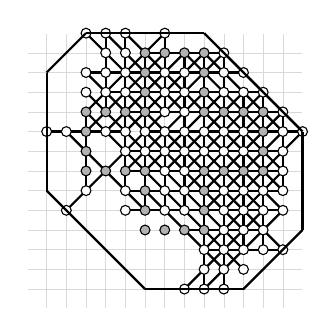
\begin{tikzpicture}[scale=0.5]
\draw[step=2*\unitsize,gray!30,very thin,shift={(-\unitsize, -\unitsize)}] (-13.900000*\unitsize,-15.900000*\unitsize) grid (13.900000*\unitsize,11.900000*\unitsize);
\tikzstyle{every node}=[draw,
			circle,
			fill=white,
			minimum size  = 0.5*\unitsize,
			node distance = 2*\unitsize,
			inner sep=0pt
			] 


\draw[thick] (-9*\unitsize,-1*\unitsize) -- (-9*\unitsize,1*\unitsize);
    

\draw[thick] (-9*\unitsize,1*\unitsize) -- (-9*\unitsize,3*\unitsize);
    

\draw[thick] (-9*\unitsize,-1*\unitsize) -- (-9*\unitsize,-3*\unitsize);
    

\draw[thick] (-9*\unitsize,-3*\unitsize) -- (-9*\unitsize,-5*\unitsize);
    

\draw[thick] (-5*\unitsize,5*\unitsize) -- (-3*\unitsize,7*\unitsize);
    

\draw[thick] (-3*\unitsize,7*\unitsize) -- (-1*\unitsize,9*\unitsize);
    

\draw[thick] (-5*\unitsize,5*\unitsize) -- (-7*\unitsize,3*\unitsize);
    

\draw[thick] (-7*\unitsize,3*\unitsize) -- (-9*\unitsize,1*\unitsize);
    

\draw[thick] (-3*\unitsize,5*\unitsize) -- (-3*\unitsize,7*\unitsize);
    

\draw[thick] (-3*\unitsize,7*\unitsize) -- (-3*\unitsize,9*\unitsize);
    

\draw[thick] (-3*\unitsize,5*\unitsize) -- (-3*\unitsize,3*\unitsize);
    

\draw[thick] (-3*\unitsize,3*\unitsize) -- (-3*\unitsize,1*\unitsize);
    

\draw[thick] (3*\unitsize,5*\unitsize) -- (3*\unitsize,7*\unitsize);
    

\draw[thick] (3*\unitsize,7*\unitsize) -- (3*\unitsize,9*\unitsize);
    

\draw[thick] (3*\unitsize,5*\unitsize) -- (3*\unitsize,3*\unitsize);
    

\draw[thick] (3*\unitsize,3*\unitsize) -- (3*\unitsize,1*\unitsize);
    

\draw[thick] (5*\unitsize,5*\unitsize) -- (7*\unitsize,3*\unitsize);
    

\draw[thick] (7*\unitsize,3*\unitsize) -- (9*\unitsize,1*\unitsize);
    

\draw[thick] (5*\unitsize,5*\unitsize) -- (3*\unitsize,7*\unitsize);
    

\draw[thick] (3*\unitsize,7*\unitsize) -- (1*\unitsize,9*\unitsize);
    

\draw[thick] (1*\unitsize,9*\unitsize) -- (3*\unitsize,9*\unitsize);
    

\draw[thick] (3*\unitsize,9*\unitsize) -- (5*\unitsize,9*\unitsize);
    

\draw[thick] (1*\unitsize,9*\unitsize) -- (-1*\unitsize,9*\unitsize);
    

\draw[thick] (-1*\unitsize,9*\unitsize) -- (-3*\unitsize,9*\unitsize);
    

\draw[thick] (9*\unitsize,1*\unitsize) -- (9*\unitsize,3*\unitsize);
    

\draw[thick] (9*\unitsize,3*\unitsize) -- (9*\unitsize,5*\unitsize);
    

\draw[thick] (9*\unitsize,1*\unitsize) -- (9*\unitsize,-1*\unitsize);
    

\draw[thick] (9*\unitsize,-1*\unitsize) -- (9*\unitsize,-3*\unitsize);
    

\draw[thick] (7*\unitsize,-3*\unitsize) -- (9*\unitsize,-3*\unitsize);
    

\draw[thick] (9*\unitsize,-3*\unitsize) -- (11*\unitsize,-3*\unitsize);
    

\draw[thick] (7*\unitsize,-3*\unitsize) -- (5*\unitsize,-3*\unitsize);
    

\draw[thick] (5*\unitsize,-3*\unitsize) -- (3*\unitsize,-3*\unitsize);
    

\draw[thick] (7*\unitsize,3*\unitsize) -- (9*\unitsize,3*\unitsize);
    

\draw[thick] (9*\unitsize,3*\unitsize) -- (11*\unitsize,3*\unitsize);
    

\draw[thick] (7*\unitsize,3*\unitsize) -- (5*\unitsize,3*\unitsize);
    

\draw[thick] (5*\unitsize,3*\unitsize) -- (3*\unitsize,3*\unitsize);
    

\draw[thick] (-3*\unitsize,-3*\unitsize) -- (-3*\unitsize,-1*\unitsize);
    

\draw[thick] (-3*\unitsize,-1*\unitsize) -- (-3*\unitsize,1*\unitsize);
    

\draw[thick] (-3*\unitsize,-3*\unitsize) -- (-3*\unitsize,-5*\unitsize);
    

\draw[thick] (-3*\unitsize,-5*\unitsize) -- (-3*\unitsize,-7*\unitsize);
    

\draw[thick] (3*\unitsize,-3*\unitsize) -- (3*\unitsize,-1*\unitsize);
    

\draw[thick] (3*\unitsize,-1*\unitsize) -- (3*\unitsize,1*\unitsize);
    

\draw[thick] (3*\unitsize,-3*\unitsize) -- (3*\unitsize,-5*\unitsize);
    

\draw[thick] (3*\unitsize,-5*\unitsize) -- (3*\unitsize,-7*\unitsize);
    

\draw[thick] (7*\unitsize,-1*\unitsize) -- (9*\unitsize,1*\unitsize);
    

\draw[thick] (9*\unitsize,1*\unitsize) -- (11*\unitsize,3*\unitsize);
    

\draw[thick] (7*\unitsize,-1*\unitsize) -- (5*\unitsize,-3*\unitsize);
    

\draw[thick] (5*\unitsize,-3*\unitsize) -- (3*\unitsize,-5*\unitsize);
    

\draw[thick] (7*\unitsize,1*\unitsize) -- (9*\unitsize,-1*\unitsize);
    

\draw[thick] (9*\unitsize,-1*\unitsize) -- (11*\unitsize,-3*\unitsize);
    

\draw[thick] (7*\unitsize,1*\unitsize) -- (5*\unitsize,3*\unitsize);
    

\draw[thick] (5*\unitsize,3*\unitsize) -- (3*\unitsize,5*\unitsize);
    

\draw[thick] (7*\unitsize,1*\unitsize) -- (7*\unitsize,3*\unitsize);
    

\draw[thick] (7*\unitsize,3*\unitsize) -- (7*\unitsize,5*\unitsize);
    

\draw[thick] (7*\unitsize,1*\unitsize) -- (7*\unitsize,-1*\unitsize);
    

\draw[thick] (7*\unitsize,-1*\unitsize) -- (7*\unitsize,-3*\unitsize);
    

\draw[thick] (5*\unitsize,5*\unitsize) -- (7*\unitsize,5*\unitsize);
    

\draw[thick] (7*\unitsize,5*\unitsize) -- (9*\unitsize,5*\unitsize);
    

\draw[thick] (5*\unitsize,5*\unitsize) -- (3*\unitsize,5*\unitsize);
    

\draw[thick] (3*\unitsize,5*\unitsize) -- (1*\unitsize,5*\unitsize);
    

\draw[thick] (1*\unitsize,5*\unitsize) -- (3*\unitsize,7*\unitsize);
    

\draw[thick] (3*\unitsize,7*\unitsize) -- (5*\unitsize,9*\unitsize);
    

\draw[thick] (1*\unitsize,5*\unitsize) -- (-1*\unitsize,3*\unitsize);
    

\draw[thick] (-1*\unitsize,3*\unitsize) -- (-3*\unitsize,1*\unitsize);
    

\draw[thick] (-1*\unitsize,3*\unitsize) -- (1*\unitsize,3*\unitsize);
    

\draw[thick] (1*\unitsize,3*\unitsize) -- (3*\unitsize,3*\unitsize);
    

\draw[thick] (-1*\unitsize,3*\unitsize) -- (-3*\unitsize,3*\unitsize);
    

\draw[thick] (-3*\unitsize,3*\unitsize) -- (-5*\unitsize,3*\unitsize);
    

\draw[thick] (-1*\unitsize,1*\unitsize) -- (1*\unitsize,3*\unitsize);
    

\draw[thick] (1*\unitsize,3*\unitsize) -- (3*\unitsize,5*\unitsize);
    

\draw[thick] (-1*\unitsize,1*\unitsize) -- (-3*\unitsize,-1*\unitsize);
    

\draw[thick] (-3*\unitsize,-1*\unitsize) -- (-5*\unitsize,-3*\unitsize);
    

\draw[thick] (-1*\unitsize,1*\unitsize) -- (1*\unitsize,-1*\unitsize);
    

\draw[thick] (1*\unitsize,-1*\unitsize) -- (3*\unitsize,-3*\unitsize);
    

\draw[thick] (-1*\unitsize,1*\unitsize) -- (-3*\unitsize,3*\unitsize);
    

\draw[thick] (-3*\unitsize,3*\unitsize) -- (-5*\unitsize,5*\unitsize);
    

\draw[thick] (3*\unitsize,1*\unitsize) -- (5*\unitsize,3*\unitsize);
    

\draw[thick] (5*\unitsize,3*\unitsize) -- (7*\unitsize,5*\unitsize);
    

\draw[thick] (3*\unitsize,1*\unitsize) -- (1*\unitsize,-1*\unitsize);
    

\draw[thick] (1*\unitsize,-1*\unitsize) -- (-1*\unitsize,-3*\unitsize);
    

\draw[thick] (-1*\unitsize,-3*\unitsize) -- (1*\unitsize,-3*\unitsize);
    

\draw[thick] (1*\unitsize,-3*\unitsize) -- (3*\unitsize,-3*\unitsize);
    

\draw[thick] (-1*\unitsize,-3*\unitsize) -- (-3*\unitsize,-3*\unitsize);
    

\draw[thick] (-3*\unitsize,-3*\unitsize) -- (-5*\unitsize,-3*\unitsize);
    

\draw[thick] (5*\unitsize,1*\unitsize) -- (7*\unitsize,3*\unitsize);
    

\draw[thick] (7*\unitsize,3*\unitsize) -- (9*\unitsize,5*\unitsize);
    

\draw[thick] (5*\unitsize,1*\unitsize) -- (3*\unitsize,-1*\unitsize);
    

\draw[thick] (3*\unitsize,-1*\unitsize) -- (1*\unitsize,-3*\unitsize);
    

\draw[thick] (1*\unitsize,1*\unitsize) -- (3*\unitsize,1*\unitsize);
    

\draw[thick] (3*\unitsize,1*\unitsize) -- (5*\unitsize,1*\unitsize);
    

\draw[thick] (1*\unitsize,1*\unitsize) -- (-1*\unitsize,1*\unitsize);
    

\draw[thick] (-1*\unitsize,1*\unitsize) -- (-3*\unitsize,1*\unitsize);
    

\draw[thick] (5*\unitsize,5*\unitsize) -- (5*\unitsize,7*\unitsize);
    

\draw[thick] (5*\unitsize,7*\unitsize) -- (5*\unitsize,9*\unitsize);
    

\draw[thick] (5*\unitsize,5*\unitsize) -- (5*\unitsize,3*\unitsize);
    

\draw[thick] (5*\unitsize,3*\unitsize) -- (5*\unitsize,1*\unitsize);
    

\draw[thick] (7*\unitsize,-1*\unitsize) -- (9*\unitsize,-3*\unitsize);
    

\draw[thick] (9*\unitsize,-3*\unitsize) -- (11*\unitsize,-5*\unitsize);
    

\draw[thick] (7*\unitsize,-1*\unitsize) -- (5*\unitsize,1*\unitsize);
    

\draw[thick] (5*\unitsize,1*\unitsize) -- (3*\unitsize,3*\unitsize);
    

\draw[thick] (1*\unitsize,1*\unitsize) -- (3*\unitsize,3*\unitsize);
    

\draw[thick] (3*\unitsize,3*\unitsize) -- (5*\unitsize,5*\unitsize);
    

\draw[thick] (1*\unitsize,1*\unitsize) -- (-1*\unitsize,-1*\unitsize);
    

\draw[thick] (-1*\unitsize,-1*\unitsize) -- (-3*\unitsize,-3*\unitsize);
    

\draw[thick] (1*\unitsize,5*\unitsize) -- (1*\unitsize,7*\unitsize);
    

\draw[thick] (1*\unitsize,7*\unitsize) -- (1*\unitsize,9*\unitsize);
    

\draw[thick] (1*\unitsize,5*\unitsize) -- (1*\unitsize,3*\unitsize);
    

\draw[thick] (1*\unitsize,3*\unitsize) -- (1*\unitsize,1*\unitsize);
    

\draw[thick] (7*\unitsize,5*\unitsize) -- (9*\unitsize,3*\unitsize);
    

\draw[thick] (9*\unitsize,3*\unitsize) -- (11*\unitsize,1*\unitsize);
    

\draw[thick] (7*\unitsize,5*\unitsize) -- (5*\unitsize,7*\unitsize);
    

\draw[thick] (5*\unitsize,7*\unitsize) -- (3*\unitsize,9*\unitsize);
    

\draw[thick] (-1*\unitsize,-1*\unitsize) -- (1*\unitsize,-1*\unitsize);
    

\draw[thick] (1*\unitsize,-1*\unitsize) -- (3*\unitsize,-1*\unitsize);
    

\draw[thick] (-1*\unitsize,-1*\unitsize) -- (-3*\unitsize,-1*\unitsize);
    

\draw[thick] (-3*\unitsize,-1*\unitsize) -- (-5*\unitsize,-1*\unitsize);
    

\draw[thick] (7*\unitsize,-3*\unitsize) -- (9*\unitsize,-1*\unitsize);
    

\draw[thick] (9*\unitsize,-1*\unitsize) -- (11*\unitsize,1*\unitsize);
    

\draw[thick] (7*\unitsize,-3*\unitsize) -- (5*\unitsize,-5*\unitsize);
    

\draw[thick] (5*\unitsize,-5*\unitsize) -- (3*\unitsize,-7*\unitsize);
    

\draw[thick] (11*\unitsize,-1*\unitsize) -- (11*\unitsize,1*\unitsize);
    

\draw[thick] (11*\unitsize,1*\unitsize) -- (11*\unitsize,3*\unitsize);
    

\draw[thick] (11*\unitsize,-1*\unitsize) -- (11*\unitsize,-3*\unitsize);
    

\draw[thick] (11*\unitsize,-3*\unitsize) -- (11*\unitsize,-5*\unitsize);
    

\draw[thick] (9*\unitsize,1*\unitsize) -- (11*\unitsize,1*\unitsize);
    

\draw[thick] (11*\unitsize,1*\unitsize) -- (13*\unitsize,1*\unitsize);
    

\draw[thick] (9*\unitsize,1*\unitsize) -- (7*\unitsize,1*\unitsize);
    

\draw[thick] (7*\unitsize,1*\unitsize) -- (5*\unitsize,1*\unitsize);
    

\draw[thick] (-7*\unitsize,-3*\unitsize) -- (-5*\unitsize,-1*\unitsize);
    

\draw[thick] (-5*\unitsize,-1*\unitsize) -- (-3*\unitsize,1*\unitsize);
    

\draw[thick] (-7*\unitsize,-3*\unitsize) -- (-9*\unitsize,-5*\unitsize);
    

\draw[thick] (-9*\unitsize,-5*\unitsize) -- (-11*\unitsize,-7*\unitsize);
    

\draw[thick] (7*\unitsize,-1*\unitsize) -- (9*\unitsize,-1*\unitsize);
    

\draw[thick] (9*\unitsize,-1*\unitsize) -- (11*\unitsize,-1*\unitsize);
    

\draw[thick] (7*\unitsize,-1*\unitsize) -- (5*\unitsize,-1*\unitsize);
    

\draw[thick] (5*\unitsize,-1*\unitsize) -- (3*\unitsize,-1*\unitsize);
    

\draw[thick] (9*\unitsize,5*\unitsize) -- (11*\unitsize,3*\unitsize);
    

\draw[thick] (11*\unitsize,3*\unitsize) -- (13*\unitsize,1*\unitsize);
    

\draw[thick] (9*\unitsize,5*\unitsize) -- (7*\unitsize,7*\unitsize);
    

\draw[thick] (7*\unitsize,7*\unitsize) -- (5*\unitsize,9*\unitsize);
    

\draw[thick] (3*\unitsize,7*\unitsize) -- (5*\unitsize,7*\unitsize);
    

\draw[thick] (5*\unitsize,7*\unitsize) -- (7*\unitsize,7*\unitsize);
    

\draw[thick] (3*\unitsize,7*\unitsize) -- (1*\unitsize,7*\unitsize);
    

\draw[thick] (1*\unitsize,7*\unitsize) -- (-1*\unitsize,7*\unitsize);
    

\draw[thick] (5*\unitsize,-1*\unitsize) -- (7*\unitsize,1*\unitsize);
    

\draw[thick] (7*\unitsize,1*\unitsize) -- (9*\unitsize,3*\unitsize);
    

\draw[thick] (5*\unitsize,-1*\unitsize) -- (3*\unitsize,-3*\unitsize);
    

\draw[thick] (3*\unitsize,-3*\unitsize) -- (1*\unitsize,-5*\unitsize);
    

\draw[thick] (5*\unitsize,-3*\unitsize) -- (5*\unitsize,-1*\unitsize);
    

\draw[thick] (5*\unitsize,-1*\unitsize) -- (5*\unitsize,1*\unitsize);
    

\draw[thick] (5*\unitsize,-3*\unitsize) -- (5*\unitsize,-5*\unitsize);
    

\draw[thick] (5*\unitsize,-5*\unitsize) -- (5*\unitsize,-7*\unitsize);
    

\draw[thick] (-3*\unitsize,5*\unitsize) -- (-1*\unitsize,7*\unitsize);
    

\draw[thick] (-1*\unitsize,7*\unitsize) -- (1*\unitsize,9*\unitsize);
    

\draw[thick] (-3*\unitsize,5*\unitsize) -- (-5*\unitsize,3*\unitsize);
    

\draw[thick] (-5*\unitsize,3*\unitsize) -- (-7*\unitsize,1*\unitsize);
    

\draw[thick] (-1*\unitsize,7*\unitsize) -- (1*\unitsize,5*\unitsize);
    

\draw[thick] (1*\unitsize,5*\unitsize) -- (3*\unitsize,3*\unitsize);
    

\draw[thick] (-1*\unitsize,7*\unitsize) -- (-3*\unitsize,9*\unitsize);
    

\draw[thick] (-3*\unitsize,9*\unitsize) -- (-5*\unitsize,11*\unitsize);
    

\draw[thick] (1*\unitsize,-3*\unitsize) -- (1*\unitsize,-1*\unitsize);
    

\draw[thick] (1*\unitsize,-1*\unitsize) -- (1*\unitsize,1*\unitsize);
    

\draw[thick] (1*\unitsize,-3*\unitsize) -- (1*\unitsize,-5*\unitsize);
    

\draw[thick] (1*\unitsize,-5*\unitsize) -- (1*\unitsize,-7*\unitsize);
    

\draw[thick] (3*\unitsize,-5*\unitsize) -- (5*\unitsize,-7*\unitsize);
    

\draw[thick] (5*\unitsize,-7*\unitsize) -- (7*\unitsize,-9*\unitsize);
    

\draw[thick] (3*\unitsize,-5*\unitsize) -- (1*\unitsize,-3*\unitsize);
    

\draw[thick] (1*\unitsize,-3*\unitsize) -- (-1*\unitsize,-1*\unitsize);
    

\draw[thick] (9*\unitsize,-3*\unitsize) -- (11*\unitsize,-1*\unitsize);
    

\draw[thick] (11*\unitsize,-1*\unitsize) -- (13*\unitsize,1*\unitsize);
    

\draw[thick] (9*\unitsize,-3*\unitsize) -- (7*\unitsize,-5*\unitsize);
    

\draw[thick] (7*\unitsize,-5*\unitsize) -- (5*\unitsize,-7*\unitsize);
    

\draw[thick] (-5*\unitsize,-1*\unitsize) -- (-3*\unitsize,-3*\unitsize);
    

\draw[thick] (-3*\unitsize,-3*\unitsize) -- (-1*\unitsize,-5*\unitsize);
    

\draw[thick] (-5*\unitsize,-1*\unitsize) -- (-7*\unitsize,1*\unitsize);
    

\draw[thick] (-7*\unitsize,1*\unitsize) -- (-9*\unitsize,3*\unitsize);
    

\draw[thick] (5*\unitsize,-3*\unitsize) -- (7*\unitsize,-5*\unitsize);
    

\draw[thick] (7*\unitsize,-5*\unitsize) -- (9*\unitsize,-7*\unitsize);
    

\draw[thick] (5*\unitsize,-3*\unitsize) -- (3*\unitsize,-1*\unitsize);
    

\draw[thick] (3*\unitsize,-1*\unitsize) -- (1*\unitsize,1*\unitsize);
    

\draw[thick] (7*\unitsize,-5*\unitsize) -- (9*\unitsize,-5*\unitsize);
    

\draw[thick] (9*\unitsize,-5*\unitsize) -- (11*\unitsize,-5*\unitsize);
    

\draw[thick] (7*\unitsize,-5*\unitsize) -- (5*\unitsize,-5*\unitsize);
    

\draw[thick] (5*\unitsize,-5*\unitsize) -- (3*\unitsize,-5*\unitsize);
    

\draw[thick] (-1*\unitsize,-5*\unitsize) -- (1*\unitsize,-5*\unitsize);
    

\draw[thick] (1*\unitsize,-5*\unitsize) -- (3*\unitsize,-5*\unitsize);
    

\draw[thick] (-1*\unitsize,-5*\unitsize) -- (-3*\unitsize,-5*\unitsize);
    

\draw[thick] (-3*\unitsize,-5*\unitsize) -- (-5*\unitsize,-5*\unitsize);
    

\draw[thick] (-1*\unitsize,-3*\unitsize) -- (-1*\unitsize,-1*\unitsize);
    

\draw[thick] (-1*\unitsize,-1*\unitsize) -- (-1*\unitsize,1*\unitsize);
    

\draw[thick] (-1*\unitsize,-3*\unitsize) -- (-1*\unitsize,-5*\unitsize);
    

\draw[thick] (-1*\unitsize,-5*\unitsize) -- (-1*\unitsize,-7*\unitsize);
    

\draw[thick] (7*\unitsize,-3*\unitsize) -- (9*\unitsize,-5*\unitsize);
    

\draw[thick] (9*\unitsize,-5*\unitsize) -- (11*\unitsize,-7*\unitsize);
    

\draw[thick] (7*\unitsize,-3*\unitsize) -- (5*\unitsize,-1*\unitsize);
    

\draw[thick] (5*\unitsize,-1*\unitsize) -- (3*\unitsize,1*\unitsize);
    

\draw[thick] (-7*\unitsize,-3*\unitsize) -- (-5*\unitsize,-5*\unitsize);
    

\draw[thick] (-5*\unitsize,-5*\unitsize) -- (-3*\unitsize,-7*\unitsize);
    

\draw[thick] (-7*\unitsize,-3*\unitsize) -- (-9*\unitsize,-1*\unitsize);
    

\draw[thick] (-9*\unitsize,-1*\unitsize) -- (-11*\unitsize,1*\unitsize);
    

\draw[thick] (-1*\unitsize,-7*\unitsize) -- (1*\unitsize,-7*\unitsize);
    

\draw[thick] (1*\unitsize,-7*\unitsize) -- (3*\unitsize,-7*\unitsize);
    

\draw[thick] (-1*\unitsize,-7*\unitsize) -- (-3*\unitsize,-7*\unitsize);
    

\draw[thick] (-3*\unitsize,-7*\unitsize) -- (-5*\unitsize,-7*\unitsize);
    

\draw[thick] (-5*\unitsize,-1*\unitsize) -- (-5*\unitsize,1*\unitsize);
    

\draw[thick] (-5*\unitsize,1*\unitsize) -- (-5*\unitsize,3*\unitsize);
    

\draw[thick] (-5*\unitsize,-1*\unitsize) -- (-5*\unitsize,-3*\unitsize);
    

\draw[thick] (-5*\unitsize,-3*\unitsize) -- (-5*\unitsize,-5*\unitsize);
    

\draw[thick] (7*\unitsize,-7*\unitsize) -- (9*\unitsize,-7*\unitsize);
    

\draw[thick] (9*\unitsize,-7*\unitsize) -- (11*\unitsize,-7*\unitsize);
    

\draw[thick] (7*\unitsize,-7*\unitsize) -- (5*\unitsize,-7*\unitsize);
    

\draw[thick] (5*\unitsize,-7*\unitsize) -- (3*\unitsize,-7*\unitsize);
    

\draw[thick] (-9*\unitsize,1*\unitsize) -- (-7*\unitsize,1*\unitsize);
    

\draw[thick] (-7*\unitsize,1*\unitsize) -- (-5*\unitsize,1*\unitsize);
    

\draw[thick] (-9*\unitsize,1*\unitsize) -- (-11*\unitsize,1*\unitsize);
    

\draw[thick] (-11*\unitsize,1*\unitsize) -- (-13*\unitsize,1*\unitsize);
    

\draw[thick] (-5*\unitsize,1*\unitsize) -- (-3*\unitsize,-1*\unitsize);
    

\draw[thick] (-3*\unitsize,-1*\unitsize) -- (-1*\unitsize,-3*\unitsize);
    

\draw[thick] (-5*\unitsize,1*\unitsize) -- (-7*\unitsize,3*\unitsize);
    

\draw[thick] (-7*\unitsize,3*\unitsize) -- (-9*\unitsize,5*\unitsize);
    

\draw[thick] (-1*\unitsize,5*\unitsize) -- (1*\unitsize,7*\unitsize);
    

\draw[thick] (1*\unitsize,7*\unitsize) -- (3*\unitsize,9*\unitsize);
    

\draw[thick] (-1*\unitsize,5*\unitsize) -- (-3*\unitsize,3*\unitsize);
    

\draw[thick] (-3*\unitsize,3*\unitsize) -- (-5*\unitsize,1*\unitsize);
    

\draw[thick] (7*\unitsize,-7*\unitsize) -- (7*\unitsize,-5*\unitsize);
    

\draw[thick] (7*\unitsize,-5*\unitsize) -- (7*\unitsize,-3*\unitsize);
    

\draw[thick] (7*\unitsize,-7*\unitsize) -- (7*\unitsize,-9*\unitsize);
    

\draw[thick] (7*\unitsize,-9*\unitsize) -- (7*\unitsize,-11*\unitsize);
    

\draw[thick] (-3*\unitsize,5*\unitsize) -- (-1*\unitsize,5*\unitsize);
    

\draw[thick] (-1*\unitsize,5*\unitsize) -- (1*\unitsize,5*\unitsize);
    

\draw[thick] (-3*\unitsize,5*\unitsize) -- (-5*\unitsize,5*\unitsize);
    

\draw[thick] (-5*\unitsize,5*\unitsize) -- (-7*\unitsize,5*\unitsize);
    

\draw[thick] (-1*\unitsize,7*\unitsize) -- (-1*\unitsize,9*\unitsize);
    

\draw[thick] (-1*\unitsize,9*\unitsize) -- (-1*\unitsize,11*\unitsize);
    

\draw[thick] (-1*\unitsize,7*\unitsize) -- (-1*\unitsize,5*\unitsize);
    

\draw[thick] (-1*\unitsize,5*\unitsize) -- (-1*\unitsize,3*\unitsize);
    

\draw[thick] (3*\unitsize,-7*\unitsize) -- (5*\unitsize,-9*\unitsize);
    

\draw[thick] (5*\unitsize,-9*\unitsize) -- (7*\unitsize,-11*\unitsize);
    

\draw[thick] (3*\unitsize,-7*\unitsize) -- (1*\unitsize,-5*\unitsize);
    

\draw[thick] (1*\unitsize,-5*\unitsize) -- (-1*\unitsize,-3*\unitsize);
    

\draw[thick] (-5*\unitsize,3*\unitsize) -- (-3*\unitsize,1*\unitsize);
    

\draw[thick] (-3*\unitsize,1*\unitsize) -- (-1*\unitsize,-1*\unitsize);
    

\draw[thick] (-5*\unitsize,3*\unitsize) -- (-7*\unitsize,5*\unitsize);
    

\draw[thick] (-7*\unitsize,5*\unitsize) -- (-9*\unitsize,7*\unitsize);
    

\draw[thick] (-5*\unitsize,7*\unitsize) -- (-3*\unitsize,9*\unitsize);
    

\draw[thick] (-3*\unitsize,9*\unitsize) -- (-1*\unitsize,11*\unitsize);
    

\draw[thick] (-5*\unitsize,7*\unitsize) -- (-7*\unitsize,5*\unitsize);
    

\draw[thick] (-7*\unitsize,5*\unitsize) -- (-9*\unitsize,3*\unitsize);
    

\draw[thick] (7*\unitsize,-7*\unitsize) -- (9*\unitsize,-5*\unitsize);
    

\draw[thick] (9*\unitsize,-5*\unitsize) -- (11*\unitsize,-3*\unitsize);
    

\draw[thick] (7*\unitsize,-7*\unitsize) -- (5*\unitsize,-9*\unitsize);
    

\draw[thick] (5*\unitsize,-9*\unitsize) -- (3*\unitsize,-11*\unitsize);
    

\draw[thick] (5*\unitsize,-9*\unitsize) -- (7*\unitsize,-9*\unitsize);
    

\draw[thick] (7*\unitsize,-9*\unitsize) -- (9*\unitsize,-9*\unitsize);
    

\draw[thick] (5*\unitsize,-9*\unitsize) -- (3*\unitsize,-9*\unitsize);
    

\draw[thick] (3*\unitsize,-9*\unitsize) -- (1*\unitsize,-9*\unitsize);
    

\draw[thick] (-5*\unitsize,7*\unitsize) -- (-3*\unitsize,7*\unitsize);
    

\draw[thick] (-3*\unitsize,7*\unitsize) -- (-1*\unitsize,7*\unitsize);
    

\draw[thick] (-5*\unitsize,7*\unitsize) -- (-7*\unitsize,7*\unitsize);
    

\draw[thick] (-7*\unitsize,7*\unitsize) -- (-9*\unitsize,7*\unitsize);
    

\draw[thick] (-5*\unitsize,7*\unitsize) -- (-5*\unitsize,9*\unitsize);
    

\draw[thick] (-5*\unitsize,9*\unitsize) -- (-5*\unitsize,11*\unitsize);
    

\draw[thick] (-5*\unitsize,7*\unitsize) -- (-5*\unitsize,5*\unitsize);
    

\draw[thick] (-5*\unitsize,5*\unitsize) -- (-5*\unitsize,3*\unitsize);
    

\draw[thick] (1*\unitsize,-9*\unitsize) -- (3*\unitsize,-11*\unitsize);
    

\draw[thick] (3*\unitsize,-11*\unitsize) -- (5*\unitsize,-13*\unitsize);
    

\draw[thick] (1*\unitsize,-9*\unitsize) -- (-1*\unitsize,-7*\unitsize);
    

\draw[thick] (-1*\unitsize,-7*\unitsize) -- (-3*\unitsize,-5*\unitsize);
    

\draw[thick] (9*\unitsize,-7*\unitsize) -- (9*\unitsize,-5*\unitsize);
    

\draw[thick] (9*\unitsize,-5*\unitsize) -- (9*\unitsize,-3*\unitsize);
    

\draw[thick] (9*\unitsize,-7*\unitsize) -- (9*\unitsize,-9*\unitsize);
    

\draw[thick] (9*\unitsize,-9*\unitsize) -- (9*\unitsize,-11*\unitsize);
    

\draw[thick] (7*\unitsize,-7*\unitsize) -- (9*\unitsize,-9*\unitsize);
    

\draw[thick] (9*\unitsize,-9*\unitsize) -- (11*\unitsize,-11*\unitsize);
    

\draw[thick] (7*\unitsize,-7*\unitsize) -- (5*\unitsize,-5*\unitsize);
    

\draw[thick] (5*\unitsize,-5*\unitsize) -- (3*\unitsize,-3*\unitsize);
    

\draw[thick] (-3*\unitsize,7*\unitsize) -- (-1*\unitsize,5*\unitsize);
    

\draw[thick] (-1*\unitsize,5*\unitsize) -- (1*\unitsize,3*\unitsize);
    

\draw[thick] (-3*\unitsize,7*\unitsize) -- (-5*\unitsize,9*\unitsize);
    

\draw[thick] (-5*\unitsize,9*\unitsize) -- (-7*\unitsize,11*\unitsize);
    

\draw[thick] (7*\unitsize,-11*\unitsize) -- (9*\unitsize,-9*\unitsize);
    

\draw[thick] (9*\unitsize,-9*\unitsize) -- (11*\unitsize,-7*\unitsize);
    

\draw[thick] (7*\unitsize,-11*\unitsize) -- (5*\unitsize,-13*\unitsize);
    

\draw[thick] (5*\unitsize,-13*\unitsize) -- (3*\unitsize,-15*\unitsize);
    

\draw[thick] (7*\unitsize,-11*\unitsize) -- (9*\unitsize,-11*\unitsize);
    

\draw[thick] (9*\unitsize,-11*\unitsize) -- (11*\unitsize,-11*\unitsize);
    

\draw[thick] (7*\unitsize,-11*\unitsize) -- (5*\unitsize,-11*\unitsize);
    

\draw[thick] (5*\unitsize,-11*\unitsize) -- (3*\unitsize,-11*\unitsize);
    

\draw[thick] (-7*\unitsize,7*\unitsize) -- (-7*\unitsize,9*\unitsize);
    

\draw[thick] (-7*\unitsize,9*\unitsize) -- (-7*\unitsize,11*\unitsize);
    

\draw[thick] (-7*\unitsize,7*\unitsize) -- (-7*\unitsize,5*\unitsize);
    

\draw[thick] (-7*\unitsize,5*\unitsize) -- (-7*\unitsize,3*\unitsize);
    

\draw[thick] (3*\unitsize,-11*\unitsize) -- (3*\unitsize,-9*\unitsize);
    

\draw[thick] (3*\unitsize,-9*\unitsize) -- (3*\unitsize,-7*\unitsize);
    

\draw[thick] (3*\unitsize,-11*\unitsize) -- (3*\unitsize,-13*\unitsize);
    

\draw[thick] (3*\unitsize,-13*\unitsize) -- (3*\unitsize,-15*\unitsize);
    

\draw[thick] (5*\unitsize,-11*\unitsize) -- (5*\unitsize,-9*\unitsize);
    

\draw[thick] (5*\unitsize,-9*\unitsize) -- (5*\unitsize,-7*\unitsize);
    

\draw[thick] (5*\unitsize,-11*\unitsize) -- (5*\unitsize,-13*\unitsize);
    

\draw[thick] (5*\unitsize,-13*\unitsize) -- (5*\unitsize,-15*\unitsize);
    

\draw[thick] (3*\unitsize,-9*\unitsize) -- (5*\unitsize,-11*\unitsize);
    

\draw[thick] (5*\unitsize,-11*\unitsize) -- (7*\unitsize,-13*\unitsize);
    

\draw[thick] (3*\unitsize,-9*\unitsize) -- (1*\unitsize,-7*\unitsize);
    

\draw[thick] (1*\unitsize,-7*\unitsize) -- (-1*\unitsize,-5*\unitsize);
    

\draw[thick] (-5*\unitsize,7*\unitsize) -- (-3*\unitsize,5*\unitsize);
    

\draw[thick] (-3*\unitsize,5*\unitsize) -- (-1*\unitsize,3*\unitsize);
    

\draw[thick] (-5*\unitsize,7*\unitsize) -- (-7*\unitsize,9*\unitsize);
    

\draw[thick] (-7*\unitsize,9*\unitsize) -- (-9*\unitsize,11*\unitsize);
    

\draw[thick] (5*\unitsize,-11*\unitsize) -- (7*\unitsize,-9*\unitsize);
    

\draw[thick] (7*\unitsize,-9*\unitsize) -- (9*\unitsize,-7*\unitsize);
    

\draw[thick] (5*\unitsize,-11*\unitsize) -- (3*\unitsize,-13*\unitsize);
    

\draw[thick] (3*\unitsize,-13*\unitsize) -- (1*\unitsize,-15*\unitsize);
    

\node[fill=black!30, thin] at (3*\unitsize,9*\unitsize) {};
        

\node[fill=black!30, thin] at (3*\unitsize,7*\unitsize) {};
        

\node[fill=black!30, thin] at (3*\unitsize,5*\unitsize) {};
        

\node[fill=black!30, thin] at (3*\unitsize,3*\unitsize) {};
        

\node[fill=black!30, thin] at (5*\unitsize,3*\unitsize) {};
        

\node[fill=black!30, thin] at (7*\unitsize,3*\unitsize) {};
        

\node[fill=black!30, thin] at (9*\unitsize,3*\unitsize) {};
        

\node[fill=black!30, thin] at (9*\unitsize,1*\unitsize) {};
        

\node[fill=black!30, thin] at (9*\unitsize,-1*\unitsize) {};
        

\node[fill=black!30, thin] at (9*\unitsize,-3*\unitsize) {};
        

\node[fill=black!30, thin] at (7*\unitsize,-3*\unitsize) {};
        

\node[fill=black!30, thin] at (5*\unitsize,-3*\unitsize) {};
        

\node[fill=black!30, thin] at (3*\unitsize,-3*\unitsize) {};
        

\node[fill=black!30, thin] at (3*\unitsize,-5*\unitsize) {};
        

\node[fill=black!30, thin] at (3*\unitsize,-7*\unitsize) {};
        

\node[fill=black!30, thin] at (3*\unitsize,-9*\unitsize) {};
        

\node[fill=black!30, thin] at (1*\unitsize,-9*\unitsize) {};
        

\node[fill=black!30, thin] at (-1*\unitsize,-9*\unitsize) {};
        

\node[fill=black!30, thin] at (-3*\unitsize,-9*\unitsize) {};
        

\node[fill=black!30, thin] at (-3*\unitsize,-7*\unitsize) {};
        

\node[fill=black!30, thin] at (-3*\unitsize,-5*\unitsize) {};
        

\node[fill=black!30, thin] at (-3*\unitsize,-3*\unitsize) {};
        

\node[fill=black!30, thin] at (-5*\unitsize,-3*\unitsize) {};
        

\node[fill=black!30, thin] at (-7*\unitsize,-3*\unitsize) {};
        

\node[fill=black!30, thin] at (-9*\unitsize,-3*\unitsize) {};
        

\node[fill=black!30, thin] at (-9*\unitsize,-1*\unitsize) {};
        

\node[fill=black!30, thin] at (-9*\unitsize,1*\unitsize) {};
        

\node[fill=black!30, thin] at (-9*\unitsize,3*\unitsize) {};
        

\node[fill=black!30, thin] at (-7*\unitsize,3*\unitsize) {};
        

\node[fill=black!30, thin] at (-5*\unitsize,3*\unitsize) {};
        

\node[fill=black!30, thin] at (-3*\unitsize,3*\unitsize) {};
        

\node[fill=black!30, thin] at (-3*\unitsize,5*\unitsize) {};
        

\node[fill=black!30, thin] at (-3*\unitsize,7*\unitsize) {};
        

\node[fill=black!30, thin] at (-3*\unitsize,9*\unitsize) {};
        

\node[fill=black!30, thin] at (-1*\unitsize,9*\unitsize) {};
        

\node[fill=black!30, thin] at (1*\unitsize,9*\unitsize) {};
        

\node[thin] at (-9*\unitsize,-5*\unitsize)  {\scalebox{0.35}{}};
            

\node[thin] at (-5*\unitsize,5*\unitsize)  {\scalebox{0.35}{}};
            

\node[thin] at (-3*\unitsize,1*\unitsize)  {\scalebox{0.35}{}};
            

\node[thin] at (3*\unitsize,1*\unitsize)  {\scalebox{0.35}{}};
            

\node[thin] at (5*\unitsize,5*\unitsize)  {\scalebox{0.35}{}};
            

\node[thin] at (5*\unitsize,9*\unitsize)  {\scalebox{0.35}{}};
            

\node[thin] at (9*\unitsize,5*\unitsize)  {\scalebox{0.35}{}};
            

\node[thin] at (11*\unitsize,-3*\unitsize)  {\scalebox{0.35}{}};
            

\node[thin] at (11*\unitsize,3*\unitsize)  {\scalebox{0.35}{}};
            

\node[thin] at (-3*\unitsize,-1*\unitsize)  {\scalebox{0.35}{}};
            

\node[thin] at (3*\unitsize,-1*\unitsize)  {\scalebox{0.35}{}};
            

\node[thin] at (7*\unitsize,-1*\unitsize)  {\scalebox{0.35}{}};
            

\node[thin] at (7*\unitsize,1*\unitsize)  {\scalebox{0.35}{}};
            

\node[thin] at (7*\unitsize,5*\unitsize)  {\scalebox{0.35}{}};
            

\node[thin] at (1*\unitsize,5*\unitsize)  {\scalebox{0.35}{}};
            

\node[thin] at (-1*\unitsize,3*\unitsize)  {\scalebox{0.35}{}};
            

\node[thin] at (1*\unitsize,3*\unitsize)  {\scalebox{0.35}{}};
            

\node[thin] at (-1*\unitsize,1*\unitsize)  {\scalebox{0.35}{}};
            

\node[thin] at (1*\unitsize,-1*\unitsize)  {\scalebox{0.35}{}};
            

\node[thin] at (-1*\unitsize,-3*\unitsize)  {\scalebox{0.35}{}};
            

\node[thin] at (1*\unitsize,-3*\unitsize)  {\scalebox{0.35}{}};
            

\node[thin] at (5*\unitsize,1*\unitsize)  {\scalebox{0.35}{}};
            

\node[thin] at (1*\unitsize,1*\unitsize)  {\scalebox{0.35}{}};
            

\node[thin] at (5*\unitsize,7*\unitsize)  {\scalebox{0.35}{}};
            

\node[thin] at (11*\unitsize,-5*\unitsize)  {\scalebox{0.35}{}};
            

\node[thin] at (-1*\unitsize,-1*\unitsize)  {\scalebox{0.35}{}};
            

\node[thin] at (1*\unitsize,7*\unitsize)  {\scalebox{0.35}{}};
            

\node[thin] at (11*\unitsize,1*\unitsize)  {\scalebox{0.35}{}};
            

\node[thin] at (-5*\unitsize,-1*\unitsize)  {\scalebox{0.35}{}};
            

\node[thin] at (5*\unitsize,-5*\unitsize)  {\scalebox{0.35}{}};
            

\node[thin] at (11*\unitsize,-1*\unitsize)  {\scalebox{0.35}{}};
            

\node[thin] at (13*\unitsize,1*\unitsize)  {\scalebox{0.35}{}};
            

\node[thin] at (-11*\unitsize,-7*\unitsize)  {\scalebox{0.35}{}};
            

\node[thin] at (5*\unitsize,-1*\unitsize)  {\scalebox{0.35}{}};
            

\node[thin] at (7*\unitsize,7*\unitsize)  {\scalebox{0.35}{}};
            

\node[thin] at (-1*\unitsize,7*\unitsize)  {\scalebox{0.35}{}};
            

\node[thin] at (1*\unitsize,-5*\unitsize)  {\scalebox{0.35}{}};
            

\node[thin] at (5*\unitsize,-7*\unitsize)  {\scalebox{0.35}{}};
            

\node[thin] at (-7*\unitsize,1*\unitsize)  {\scalebox{0.35}{}};
            

\node[thin] at (-5*\unitsize,11*\unitsize)  {\scalebox{0.35}{}};
            

\node[thin] at (1*\unitsize,-7*\unitsize)  {\scalebox{0.35}{}};
            

\node[thin] at (7*\unitsize,-9*\unitsize)  {\scalebox{0.35}{}};
            

\node[thin] at (7*\unitsize,-5*\unitsize)  {\scalebox{0.35}{}};
            

\node[thin] at (-1*\unitsize,-5*\unitsize)  {\scalebox{0.35}{}};
            

\node[thin] at (9*\unitsize,-7*\unitsize)  {\scalebox{0.35}{}};
            

\node[thin] at (9*\unitsize,-5*\unitsize)  {\scalebox{0.35}{}};
            

\node[thin] at (-5*\unitsize,-5*\unitsize)  {\scalebox{0.35}{}};
            

\node[thin] at (-1*\unitsize,-7*\unitsize)  {\scalebox{0.35}{}};
            

\node[thin] at (11*\unitsize,-7*\unitsize)  {\scalebox{0.35}{}};
            

\node[thin] at (-11*\unitsize,1*\unitsize)  {\scalebox{0.35}{}};
            

\node[thin] at (-5*\unitsize,-7*\unitsize)  {\scalebox{0.35}{}};
            

\node[thin] at (-5*\unitsize,1*\unitsize)  {\scalebox{0.35}{}};
            

\node[thin] at (7*\unitsize,-7*\unitsize)  {\scalebox{0.35}{}};
            

\node[thin] at (-13*\unitsize,1*\unitsize)  {\scalebox{0.35}{}};
            

\node[thin] at (-9*\unitsize,5*\unitsize)  {\scalebox{0.35}{}};
            

\node[thin] at (-1*\unitsize,5*\unitsize)  {\scalebox{0.35}{}};
            

\node[thin] at (7*\unitsize,-11*\unitsize)  {\scalebox{0.35}{}};
            

\node[thin] at (-7*\unitsize,5*\unitsize)  {\scalebox{0.35}{}};
            

\node[thin] at (-1*\unitsize,11*\unitsize)  {\scalebox{0.35}{}};
            

\node[thin] at (5*\unitsize,-9*\unitsize)  {\scalebox{0.35}{}};
            

\node[thin] at (-9*\unitsize,7*\unitsize)  {\scalebox{0.35}{}};
            

\node[thin] at (-5*\unitsize,7*\unitsize)  {\scalebox{0.35}{}};
            

\node[thin] at (3*\unitsize,-11*\unitsize)  {\scalebox{0.35}{}};
            

\node[thin] at (9*\unitsize,-9*\unitsize)  {\scalebox{0.35}{}};
            

\node[thin] at (-7*\unitsize,7*\unitsize)  {\scalebox{0.35}{}};
            

\node[thin] at (-5*\unitsize,9*\unitsize)  {\scalebox{0.35}{}};
            

\node[thin] at (5*\unitsize,-13*\unitsize)  {\scalebox{0.35}{}};
            

\node[thin] at (9*\unitsize,-11*\unitsize)  {\scalebox{0.35}{}};
            

\node[thin] at (11*\unitsize,-11*\unitsize)  {\scalebox{0.35}{}};
            

\node[thin] at (-7*\unitsize,11*\unitsize)  {\scalebox{0.35}{}};
            

\node[thin] at (3*\unitsize,-15*\unitsize)  {\scalebox{0.35}{}};
            

\node[thin] at (5*\unitsize,-11*\unitsize)  {\scalebox{0.35}{}};
            

\node[thin] at (-7*\unitsize,9*\unitsize)  {\scalebox{0.35}{}};
            

\node[thin] at (3*\unitsize,-13*\unitsize)  {\scalebox{0.35}{}};
            

\node[thin] at (5*\unitsize,-15*\unitsize)  {\scalebox{0.35}{}};
            

\node[thin] at (7*\unitsize,-13*\unitsize)  {\scalebox{0.35}{}};
            

\node[thin] at (-9*\unitsize,11*\unitsize)  {\scalebox{0.35}{}};
            

\node[thin] at (1*\unitsize,-15*\unitsize)  {\scalebox{0.35}{}};
            
\draw[thick] (-13*\unitsize,-5*\unitsize) -- (-13*\unitsize, 7*\unitsize);
\draw[thick] (-13*\unitsize,7*\unitsize) -- (-9*\unitsize, 11*\unitsize);
\draw[thick] (-9*\unitsize, 11*\unitsize) -- (3*\unitsize, 11*\unitsize);
\draw[thick] (3*\unitsize, 11*\unitsize) -- (13*\unitsize, 1*\unitsize);
\draw[thick] (13*\unitsize, 1*\unitsize) -- (13*\unitsize, -9*\unitsize);
\draw[thick] (13*\unitsize, -9*\unitsize) -- (7*\unitsize, -15*\unitsize);
\draw[thick] (7*\unitsize, -15*\unitsize) -- (-3*\unitsize, -15*\unitsize);
\draw[thick] (-3*\unitsize, -15*\unitsize) -- (-13*\unitsize,-5*\unitsize);

\end{tikzpicture}


\end{minipage}
\end{figure}

We proved that passing to the octagonal hull of a Morpion position graph can increase its boundary size by up to $4$.

\end{frame}

\begin{frame}
\frametitle{Bound on the size of the board}

Hence every Morpion position graph is contained in an octagonal board with boundary size up to $288$ / $290$ / $292$.

\vspace{5mm}
You can enumerate all such boards - there are $126912$ of them.

\vspace{5mm}
The largest one has area of $741$ - with $36$ starting dots this gives upper bound of $705$ of Demaine et al.

\vspace{5mm}
The boards are small enough to get good linear relaxation bounds.

\end{frame}

%%%%
%
% Implementation
%
%%%%

\section{The Computation}
\subsection{Bound obtained by linear programming}

\begin{frame}
\frametitle{Linear Relaxation Bound}

There are $126912$ octagonal boards that contain all possible Morpion Solitaire positions.

\pause\vspace{8mm}
The largest linear relaxation bound of $586.82353$ was obtained for octagon with side lengths $10, 8, 10, 12, 10, 8, 10, 12$.

\end{frame}

\begin{frame}
\frametitle{Linear relaxation bound}

\begin{center}
\includegraphics[height=6cm]{positions/586.pdf}
\end{center}

\end{frame}

\begin{frame}
\frametitle{Linear Relaxation Bound}

There are $126912$ octagonal boards that contain all possible Morpion Solitaire positions.

\vspace{8mm}
The largest linear relaxation bound of $586.82353$ was obtained for octagon with side lengths $10, 8, 10, 12, 10, 8, 10, 12$.

\vspace{8mm}
The total computation time was less than $24$ hours on a single core of a modern processor.

\vspace{8mm}
The linear programming problems contain around $3000$ variables and $6500$ constraints each.
\end{frame}

\subsection{Bound obtained by mixed integer programming}

\begin{frame}[fragile]
\frametitle{MIP Bound}

Gurobi solver output for MIP version of the problem for the "hardest" case.

{\tiny
\begin{verbatim}
Root relaxation: objective 5.868235e+02, 6386 iterations, 7.81 seconds

    Nodes    |    Current Node    |     Objective Bounds      |     Work
 Expl Unexpl |  Obj  Depth IntInf | Incumbent    BestBd   Gap | It/Node Time

     0     0  586.82353    0  228          -  586.82353      -     -    9s
     0     0  585.98492    0  227          -  585.98492      -     -   12s
     0     0  584.78440    0  235          -  584.78440      -     -   17s
     0     0  583.89727    0  236          -  583.89727      -     -   20s
     0     0  583.78764    0  236          -  583.78764      -     -   22s
     0     0  583.77255    0  236          -  583.77255      -     -   23s
     0     0  583.77255    0  236          -  583.77255      -     -   24s
     0     2  583.77255    0  236          -  583.77255      -     -   35s
     2     4  578.83917    1  271          -  582.45157      -  5671   67s
     3     5  578.73120    2  532          -  582.45106      -  6229   90s
     4     6  571.89240    2  528          -  578.83917      -  6442  114s
\end{verbatim}
}

We can push the bound down by partially solving MIP versions of the linear problems with highest objectives.
\end{frame}

\begin{frame}
\frametitle{MIP Bound}

\begin{tabular}[t]{p{3cm}p{5cm}}
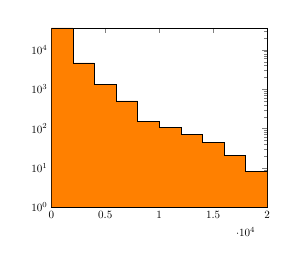
\begin{tikzpicture}[scale=0.4]
  \begin{semilogyaxis}[
    ymin=1,
    ymax=36033,
    log origin=infty,
    enlargelimits=false
  ]
    \addplot
      [const plot,fill=orange,draw=black]
      coordinates
        {(0,36033)    (2000,4644)  (4000,1302)   (6000,503)
         (8000,155) (10000,106)  (12000,71)  (14000,45)
         (16000,21) (18000,8)  (20000,1)}
  \closedcycle;
  \end{semilogyaxis}
\end{tikzpicture}
&
\raisebox{1cm}{
\parbox{5cm}{\footnotesize
The vertical axis shows the number of cases and the horizontal axis shows the computation time in seconds. 
}}
\end{tabular}

\vspace{1mm}
Out of $126912$ problems $42889$ have relaxed bound bigger or equal to $485$.

\vspace{1mm}
For $8$ problems the computation time exceeded $5$ hours.

\vspace{1mm}
The total computation time was approximately $310$ days on a single core of a modern processor.

\end{frame}

\subsection{References}
\begin{frame}
\frametitle{Source code}

A lower upper bound may be found but the whole computation has to be repeated.

\vspace{5mm}

The source code is available on github.

\vspace{5mm}
\begin{center}
\url{http://github.com/anagorko/morpion-lpp/}
\end{center}

\vspace{5mm}
Allows generation of four different relaxations (includes MIP problems whose all solutions are valid Morpion Solitaire games - much more difficult to solve), different variants of Morpion Solitaire, symmetry constraints, etc.

\end{frame}

\begin{frame}[c, plain]

\vspace{5mm}
\centering\Huge\bf
Thank you for your attention!
\end{frame}

\end{document}
